% Use the University of Michigan thesis class.
\documentclass[thesis,openany]{./tex/thesis-umich}


\newcommand*{\ATLASLATEXPATH}{latex/}
\usepackage{\ATLASLATEXPATH atlasphysics}
\usepackage{ANA-HIGG-2020-16-INT1-defs}

\RequirePackage{doi}
\usepackage{hyperref}
\usepackage{pgffor}
\usepackage{longfigure}
\usepackage{mathtools}
\usepackage{bm}
\usepackage{multirow}
\usepackage[export]{adjustbox}
\usepackage{mathrsfs}
\usepackage{float}
\usepackage{makecell}
\usepackage{lscape}
\usepackage{pdflscape}
\usepackage{amsmath}
\usepackage{xifthen}
\usepackage{rotating}
\usepackage{etoolbox}
\usepackage{tikz}

\usepackage{siunitx}
% High energy physics
\DeclareSIUnit\micron{\micro\metre}
\DeclareSIUnit\mrad{\milli\rad}
\DeclareSIUnit\gauss{G}
\DeclareSIUnit\eVperc{\eV\per\clight}
\DeclareSIUnit\nanobarn{\nano\barn}
\DeclareSIUnit\picobarn{\pico\barn}
\DeclareSIUnit\femtobarn{\femto\barn}
\DeclareSIUnit\attobarn{\atto\barn}
\DeclareSIUnit\zeptobarn{\zepto\barn}
\DeclareSIUnit\yoctobarn{\yocto\barn}
\DeclareSIUnit\nb{\nano\barn}
\DeclareSIUnit\pb{\pico\barn}
\DeclareSIUnit\fb{\femto\barn}
\DeclareSIUnit\ab{\atto\barn}
\DeclareSIUnit\zb{\zepto\barn}
\DeclareSIUnit\yb{\yocto\barn}




% Title of the thesis
\title{Precision Measurements of Higgs Boson Couplings in the Diphoton Decay Channel with Run-2 of the ATLAS Detector}

% Author name
\author{Garrett Merz}

% Department
\department{Physics}

% Year of completion
\year=2021

% ORCID ID 
\orcid{My Orcid ID}

% UM Unique Name 
\umuniquename{gwmerz}

% Frontispiece
%\frontispiece{\includegraphics[width=4in]{./pics/frontispiece.pdf}}

% Default style for front pages
\frontpagestyle{1}

% Dedication
\dedication{ “Questing Physicks isn’t like the Quiet and Queer branches. You can’t do it at home in a comfortable chair—you have to be out in the thick of the business, with your tools on your belt and your heart on your sleeve!” - Catherynne Valente, The Girl Who Fell Beneath Fairyland and Led The Revels There \cite{Fairyland}. \\}


% Acknowledgments
\acknowledgments[6]{
% The acknowledgements section of this dissertation, perhaps surprisingly, is the hardest for me to write. If left to my own devices, I have no doubt that the list of people I'd want to thank would be as long as the rest of this paper, if not longer. Like the globe held up by the Atlas of myth, my world is perched upon the shoulders of giants. Completing a dissertation at any point is no easy task, let alone in the middle of a pandemic- I could not have done this alone.

%First, to my family- to my parents, Gregg and Gretchen, thank you for working so hard to foster a lifelong sense of curiosity in me, in a world that doesn't always value it. Without the endless stream of NOVA specials, public lectures, and museum trips, I would not be the person I am today.

%To my brother Grant, thank you for 

%To my grandparents, JoAnn and Ray, Ray and Sue, and Bert and Ron- thank you for

%Most of all, of course, thanks to my partner, Abigail Goodhart, who

}
% This command sets the width of the acknowledgments area as a fraction
% of the total width of the text area.
%\acknowledgmentswidth{0.85}

% Preface
%\preface[2]{ Do I need this?}

% Committee
\committee{ %
Thomas Schwarz, Chair \\
Dante Amidei \\ 
Junjie Zhu \\ 
James Liu \\ 
Eric Bell \\ }

% Chair must be entered separately for formatting reasons.
\chair{Thomas Schwarz}

% Commands to hide or show lists of figures, tables, etc.
%\hidelistoftables
%\showlistofprograms
\showlistofappendices

% Definition of any abbreviations used.
\abbreviations{ 
    \acro{CERN}{Center for European Nuclear Research}
    \acro{ATLAS}{A Toroidal LHC ApparatuS}
    \acro{CMS}{Compact Muon Solenoid}
    \acro{LHC}{Large Hadron Collider}
    \acro{LEP}{Large Electron-Positron Collider}
    \acro{CP}{Charge-Parity}
    \acro{CPT}{Charge-Parity-Time}
    \acro{BDT}{Boosted Decision Tree}
    \acro{QCD}{Quantum Chromodynamics}
    \acro{STXS}{Simplified Template Cross-Section}
    \acro{CKM}{Cabbibo-Kobayashi-Masakawa}
    \acro{LO}{Leading Order}
    \acro{NLO}{Next-to-Leading Order}
    \acro{NNLO}{Next-to-Next-to-Leading Order}
    \acro{PDF}{Parton Distribution Function}
    \acro{SM}{Standard Model}
    \acro{BSM}{Beyond the Standard Model}
    \acro{HC}{Higgs Characterization}
    \acro{RF}{Radiofrequency}
    \acro{SPS}{Super Proton Synchrotron}
    \acro{LINAC}{Linear Accelerator}
    \acro{PSB}{Proton Synchrotron Booster}
    \acro{LHCb}{Large Hadron Collider Beauty}
    \acro{ALICE}{A Large Ion Collider Experiment}
    \acro{HL-LHC}{High-Luminosity Large Hadron Collider}
    \acro{ECAL}{Electronic Calorimeter}
    \acro{HCAL}{Hadronic Calorimeter}
    \acro{IBL}{}
    \acro{SCT}{}
    \acro{TRT}{}
    \acro{MBTS}{}
    \acro{EM}{}
    \acro{LAr}{}
    \acro{PTP}{}
    \acro{POPOP}{}
    \acro{HEC}{}
    \acro{FCAL}{}
    \acro{MDT}{}
    \acro{CSC}{}
    \acro{RPC}{}
    \acro{TGC}{}
    \acro{L1}{}
    \acro{CTP}{}
    \acro{L2}{}
    \acro{HLT}{}
    \acro{GEANT4}{}
    \acro{ID}{Identification}
    \acro{JVT}{}
    \acro{PFlow}{}
    \acro{XGBoost}{}
    \acro{TMVA}{}
    \acro{TI}{}
    \acro{NTI}{}
    \acro{NNLOPS}{}
    \acro{EFT}{}
    \acro{CB}{}
    \acro{DSCB}{}
    \acro{SS}{}
    \acro{GPR}{}
    \acro{SBBDT}{}
    \acro{CPBDT}{}
    \acro{ROC-AUC}{}
    \acro{LHAPDF}{}
    \acro{PDF4LHC}{}
    \acro{UEPS}{}
    \acro{CLs}{}
    \acro{LUCID}{}
    \acro{KLFitter}{}
    \acro{BAT}{}
    \acro{GaSBaG}{}
    \acro{RBF}{}
    \acro{GP}{}
    \acro{DoF}{}

}



% Some abstract text
\abstract{ %
My Abstract. 
}
%\hideabstractpagenumber

%% DOCUMENT AREA




\usepackage{ amssymb }
\usepackage{ amsmath }
\begin{document}

% ----- Introduction ----- %

\chapter{Introduction} \label{chap:intro}
	The discovery of the Higgs boson in 2012 by CERN's ATLAS \cite{HiggsATLAS} and CMS \cite{HiggsCMS} collaborations at the Large Hadron Collider marked a watershed moment in the history of collider physics. With its discovery, the Standard Model of particle physics, developed in the 1970s by scientists attempting to understand the deluge of new particles discovered throughout the 20th century, had finally been completed. However, countless physics questions remained (and still do remain) unanswered - why is the universe comprised of matter rather than antimatter? What are dark matter and dark energy? Can the four fundamental forces be unified?

With the Standard Model unable to provide answers to these questions, physicists have begun to search for clues in precision measurements of existing particles and their properties. Many new physics phenomena may appear as subtle hints in these measurement regimes before their eventual direct observation at the colliders of tomorrow. This has precedent in the field of Higgs physics- though predicted by the Standard Model in the 1970s, indirect evidence of the Higgs was first seen through precision measurements with the LEP experiment almost a decade before its official discovery \cite{LEPExperiments}.

One such avenue for these precision measurements using current experiements is that of the interactions of the Higgs boson with the other particles of the Standard Model. By measuring how strongly the Higgs interacts with these particles and how often its various interactions occur (parameterized mathematically using quantities called `couplings' and `cross-sections', respectively), physicists can search for experimental disagreements with the Standard Model and set limits on the allowed parameters of potential beyond-the-Standard-Model physics.

Of particular interest is the Higgs coupling to the top quark, the heaviest of all known fundamental particles. Because the Higgs couplings are intimately related to the origins of the quark and lepton masses, the coupling between the Higgs and the top is of special theoretical importance, as it can in many cases serve as a window on new physics in the Higgs sector. By observing top-quark pair production in association with a Higgs boson ($ttH$), a rare process only recently observed at the LHC \cite{ttH}, this coupling can be measured precisely and its properties ascertained.

The work in this dissertation discusses the measurement of Higgs boson processes in the diphoton decay channel ($H \rightarrow \gamma \gamma$) using proton-proton collisions with a center-of-mass energy of $\sqrt{s} = 13$ TeV, recorded with the ATLAS detector.  Both analyses presented in this dissertation use the full ATLAS Run 2 dataset, which consists of $139 fb^{-1}$ of data gathered between 2015 and 2018. Two analyses are presented- one a precision measurement of the charge-parity (CP) symmetry of the top-quark-Higgs coupling (previously published as \cite{CPanalysis}), and another a measurement of the Higgs production cross-sections for various processes in a number of theoretically-motivated kinematic regimes (previously published as \cite{Couplingsanalysis}).
 
In both analyses, measurements are performed by categorizing events gathered using the ATLAS detector into signal-enriched regions of interest using machine-learning algorithms called Boosted Decision Trees (BDTs). These tools are trained on Monte Carlo simulated data to combine the effects of multiple discriminatory variables, allowing us to focus analysis efforts on regions with a higher signal significance. In these categories, the diphoton mass distribution $m_{\gamma \gamma}$ is then fit with a smoothly-falling background functional form (which models the shape of the QCD continuum diphoton background) and a Gaussian-like ``Double-Sided Crystal Ball" signal functional form (which models the shape of the Higgs peak), and the number of fitted signal events in each category is extracted. Using the signal yields in multiple categories, various quantities of interest can be measured.

The structure of this work is as follows: first, the theoretical background and phenomenology of the Standard Model are discussed in Chapter 2. Special attention is paid to the Higgs boson and its couplings, as well as the nature of charge-parity (CP) symmetry. In Chapter 3, an overview of the construction and operation of the ATLAS detector is given. In Chapter 4, the reconstruction of particles and their properties using detector signals is elaborated upon. Chapter 5 discusses the parameters of the various data and Monte Carlo simulation samples used in the analyses. Chapter 6 details the common signal and background parameterization procedures for the two analyses discussed in this dissertation. In Chapter 7, a measurement of the CP properties of the top Yukawa coupling is outlined; the result of this measurement is presented in Chapter 8. In Chapter 9, a measurement of the Higgs boson production cross-section in a number of Simplified Template Cross-Section (STXS) kinematic regions is discussed. In Chapter 10, the conclusion chapter, the results of both analyses are discussed.
 

\chapter{An Overview of the Standard Model} \label{chap:theory_chapter}
	\section{The Standard Model} \label{sec:SM} 

The Standard Model of Particle Physics is arguably one of the crowning achievements of the last century of physics research. Though it is doubtless incomplete (it does not, for instance, explain the dark energy or dark matter observed in cosmological experiments, nor does it provide a satisfactory quantum-mechanical model of gravity), all predictions it has made have yet to be falsified \cite{Peskin}, \cite{kane_2017}, \cite{Griffiths}.

The Standard Model is a quantum field theory, meaning that it describes the behavior of fields (physical quantities that are defined at all points in spacetime; common examples of fields include electric and magnetic fields) and their discrete, quantized excitations, referred to as particles (common examples of particles are the electron and the photon, which are excitations of the "electron field" and the electromagnetic field respectively). More about the mathematics of field dynamics will be discussed in section \ref{sec:Lagrangians}.

The Standard Model divides these fundamental particles (and their corresponding fields) into two major categories: the bosons and the fermions. Fermions carry half-integer spin, while bosons carry integer spin. In a general sense, the elementary fermions can be thought of as the particles that comprise matter, while the elementary bosons can be thought of as the particles that correspond to the behavior of the four fundamental forces (electromagnetism, the strong nuclear force, the weak nuclear force, and gravity).

The elementary fermions of the Standard Model all have spin $1/2$. They are divided into two major subgroupings, quarks and leptons; each of these is further divided into three generations. Each generation of quarks contains one up-type quark (up, charm, or top) and one down-type quark (down, strange, and bottom), while each generation of leptons contains one charged lepton (electron, muon, or tau) and one neutrino (electron neutrino, muon neutrino, or tau neutrino). Fermions of successive generations behave similarly to each other, though those of each subsequent generation are more massive than the last.

The quarks are the only fermions that undergo both the strong and weak nuclear interactions, and are also the only particles in the Standard Model that have fractional electromagnetic charge ($+2/3$ for up-type quarks and $-1/3$ for down-type quarks). However, because quarks are never found in isolation and are always bound to other quarks in composite states called hadrons, all observable quark final states have integer charge. Conversely, the charged leptons all have an electromagnetic charge of $-1$, while neutrinos are chargeless. While the quarks and charged leptons have precisely-measured masses, the mass of the neutrinos is vanishingly small, and, to date, only the differences between the different neutrino masses have been conclusively measured.

In addition to these 12 fermion species, each fermion species has a corresponding antimatter "antifermion" species, which has the opposite charge and parity quantum numbers. This is discussed at length in section \ref{sec:CPT}.

The bosons of the standard model are the "messengers" through which the fundamental forces operate (with the exception of the Higgs boson, which is detailed at length in section \ref{sec:EWSB}). The photon and the gluons are massless, while the two W-bosons, the Z-boson, and the Higgs boson are all massive. The photon is the mediator of the electromagnetic force and couples to charged particles; the gluon is the mediator of the strong nuclear force and couples to particles with "color charge", and the W and Z bosons are the mediators of the weak nuclear interaction, coupling to all fermions with left-handed parity and antifermions with right-handed parity. In addition, the three weak bosons ($W^{+}$, $W^{-}$, and $Z$) can all couple to each other, as can the gluons.

The strong nuclear interaction binds quarks together, while the weak interaction governs the decay of one species of fermion into another. Weak interactions operate primarily on fermion doublets, coupling each up-type quark to its corresponding down-type quark and each charged lepton to its corresponding neutrino. However, some intergenerational coupling does occur, the rarity of which is governed by a matrix of coefficients called the Cabibbo-Kobayashi-Masakawa (or CKM) matrix \cite{CKM1}, \cite{CKM2}. 

The Higgs boson is the only scalar (spin-0) boson in the Standard Model. Though it does not mediate any force directly, its existence is a consequence of the unification of the electromagnetic and weak nuclear interactions into one "electroweak" interaction at high energy scales. Without the role of the Higgs boson in this process, the fermions, the W-bosons, and the Z-boson would all be massless; thus, the Higgs can be said to "give mass" to the particles of the Standard Model. It couples to all massive particles in the Standard Model, namely, the fermions and the W and Z bosons.

\begin{figure}
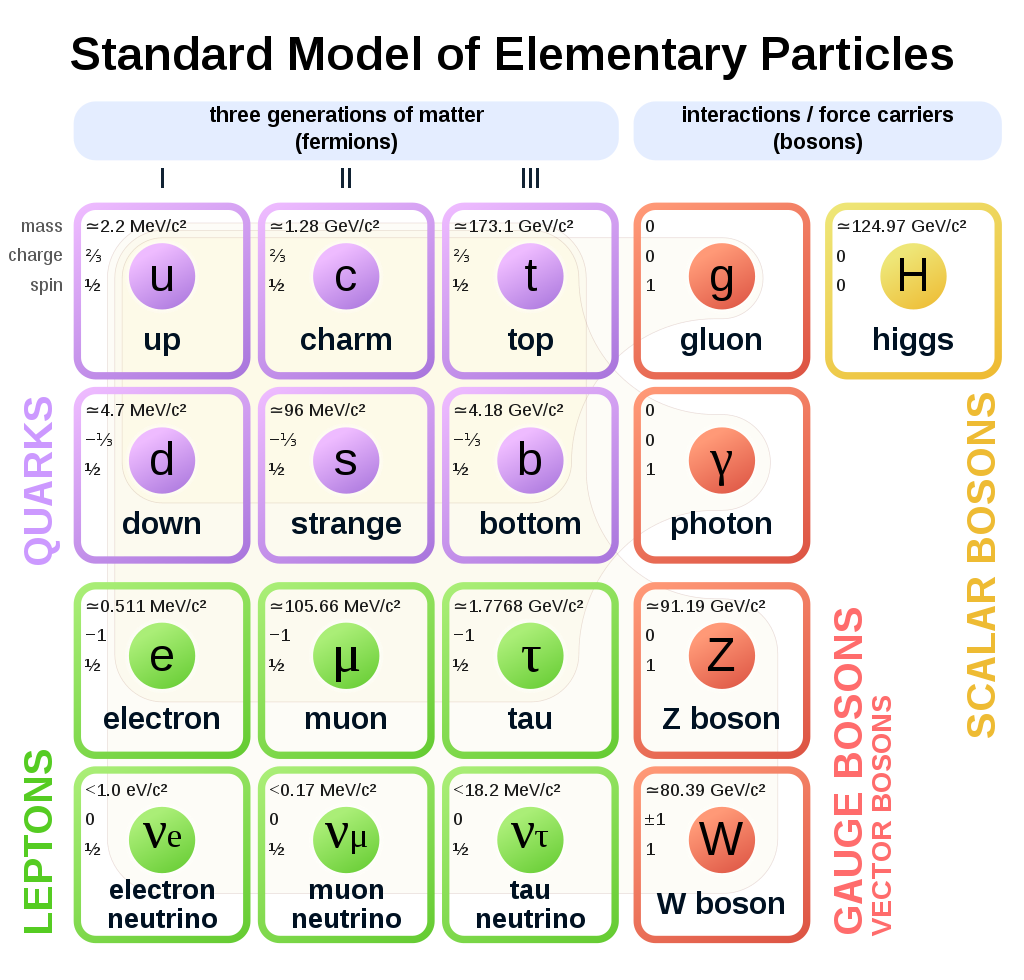
\includegraphics[width=\linewidth]{figures/theory_chapter/SM.png}
\caption{The "periodic table" of the Standard Model, depicting the three generations of fermions, the gauge bosons, and the Higgs \cite{WikipediaSM}.}
\end{figure}

\subsection{Lagrangians, Fields, and Gauge Transformations}\label{sec:Lagrangians}

In order to fully explain the Higgs mechanism, we must first discuss the mathematical language of quantum field theory. Both quantum and classical field theories are often discussed using Lagrangian dynamics, where the Lagrangian is defined as  $\mathcal{L} = T - V$, the difference of the kinetic and the potential energy. Physical properties will always evolve in such a way that the integral of this property with respect to time, $\mathcal{S} = \int \mathcal{L} dt$, called the action, is a constant. Lagrangians are also incredibly useful in that they give rise to conservation laws: Noether's Theorem states that operations performed on a system that do not change the Lagrangian are each associated to conserved quantities of a system (i.e., systems with translationally invariant Lagrangians must respect conservation of momentum, systems with temporally-invariant Lagrangians must respect conservation of energy, etc.).

A variety of types of fields exist, but we will discuss three at length: Klein-Gordon fields, which are scalar fields, Dirac spinor (vector) fields, and gauge fields (additional vector fields that must be introduced in order to preserve certain physical symmetries. We begin with the Klein-Gordon field.

Klein-Gordon fields, one of the simplest examples of a field, are real scalar-valued quantities often denoted using the symbol $\phi$. A non-interacting "free" Klein-Gordon field evolves according to the Lagrangian:

\begin{align}
  \begin{aligned}
\mathcal{L} = T - V \\
=\frac{1}{2} \frac{\partial^{2} \phi}{\partial t^{2}} - \frac{1}{2} (\nabla \phi)^{2} - \frac{1}{2} m^{2} \phi^{2} \\
=-\frac{1}{2}(\partial^{\mu}\phi)(\partial_{\mu}\phi)- \frac{1}{2} m^{2} \phi^{2}
  \end{aligned}&&&
\end{align}

where we utilize Einstein sum notation in the last line to compress the four derivatives in the preceding expression into a single shorthand symbol. The Lagrangian of an interacting Klein-Gordon field would look similar, but would possess additional $V$ potential terms depending on the nature of the interaction. As the only scalar in the Standard Model, the observable Higgs boson is the only elementary particle to follow an interacting Klein-Gordon field equation.

While the concept of a complex-valued scalar field does not directly correspond to any of the physical elementary particles that are present in the Standard Model, it plays an important role in the understanding of the Higgs mechanism. A complex-valued scalar field behaves similarly to a real-valued one, with the Lagrangian:

\begin{equation}
\mathcal{L} = (\partial^{\mu}\phi^{*})(\partial_{\mu}\phi) - \frac{1}{2} m^{2} \phi^{*} \phi
\end{equation}

Where * denotes the complex conjugate of the scalar field.

Finally, Dirac fields describe all Standard Model fermions (with the possible exception of neutrinos). They are vector fields as opposed to scalar fields, and behave according to the Lagrangian:

\begin{equation}
\mathcal{L} = \bar{\psi}(i \gamma^{\mu} \partial_{\mu} - m) \psi
\label{eq:Dirac}
\end{equation}

where $\gamma^{\mu}$ denotes the set of Dirac gamma matrices, and $\bar{\psi} = \psi^{\dag} \gamma^0$ denotes the transpose of the complex conjugate of the vector field multiplied by one of these matrices, defined as such in order to preserve invariance under relativistic Lorentz boosts. 

A four-component Dirac vector field can be written in a variety of representations, but one of the most useful is that of a doublet of two two-component Weyl spinors, one left-handed and one right-handed, that is, $\psi = \begin{pmatrix} \psi_L \\ \psi_R \end{pmatrix}$. Each of these components transforms differently under Lorentz boosts.

In order to discuss the gauge fields corresponding to the Standard Model bosons, we must first discuss the concept of gauge symmetries. Consider a single Dirac vector field described by equation \ref{eq:Dirac}. We transform the field by rotating it by a constant phase $\alpha$:  $\psi \rightarrow e^{i \alpha} \psi $, $\bar{\psi} \rightarrow e^{-i \alpha} \bar{\psi} $.

\begin{align}
  \begin{aligned}
\mathcal{L} = - (e^{-i \alpha} \bar{\psi})(i \gamma^{\mu} \partial_{\mu} - m) (e^{i \alpha} \psi) \\
= - (e^{-i \alpha} e^{i \alpha})\bar{\psi} (i \gamma^{\mu} \partial_{\mu} - m)\psi \\
= -\bar{\psi}(i \gamma^{\mu} \partial_{\mu} - m) \psi 
  \end{aligned}&&&
\end{align}

We see that we recover the original Dirac Lagrangian. Thus, the lagrangian is invariant under a constant phase rotation. A transformation of this charater is called a global gauge transformation. A one-dimensional rotation is a unitary transformation, so we call this a global $U(1)$ gauge symmetry.

We next consider the concept of a local gauge transformation, that is, one in which the phase $\alpha$ may vary with position. The field transforms, as before, like  $\psi \rightarrow e^{i \alpha (x)} \psi $, $\bar{\psi} \rightarrow e^{-i \alpha (x)} \bar{\psi} $. However, we note that the dependence on position means that we can no longer factor out the exponentials, and we thus have

\begin{align}
  \begin{aligned}
\mathcal{L} = - (e^{-i \alpha (x)} \bar{\psi})(i \gamma^{\mu} \partial_{\mu} - m) (e^{i \alpha (x)} \psi) \\
=-i e^{-i \alpha (x)} \bar{\psi} \gamma^{\mu} (e^{i \alpha (x)} \partial_{\mu} \psi  + i e^{i \alpha (x)} \psi \partial_{\mu} \alpha -m \bar{\psi}\psi \\
=-\bar{\psi}(i \gamma^{\mu} \partial_{\mu} + \gamma^{\mu} \partial_{\mu} \alpha - m) \psi
  \end{aligned}&&&
\end{align}

i.e., the Lagrangian is not invariant under this sort of transformation. However, local gauge invariance is an important physical symmetry, so in order to attempt to preserve it, we add an additional term to the original Lagrangian: an extra vector field $A_\mu$ that transforms like $A_\mu \rightarrow A_\mu - \frac{1}{q} \partial_{\mu} \alpha(x) $ for a constant q. We also define a new operator, called the covariant derivative: $D_{\mu} = \partial_{\mu}+ iqA_{\mu} $. Given how $A_{\mu}$ transforms, we see that $D_{\mu}$ transforms like

\begin{align}
  \begin{aligned}
D_{\mu} = \partial_\mu + iqA_{\mu} \\
\rightarrow \partial_\mu + iq(A_{\mu}-\frac{1}{q}\partial_{\mu}\alpha(x)) \\
= \partial_\mu + iqA_{\mu}-i\partial_{\mu}\alpha(x) \\
=D_{\mu}-i\partial_{\mu}\alpha(x)
  \end{aligned}&&&
\end{align}

Let us replace the $\partial_{\mu}\phi$ terms in the initial Lagrangian with $D_{\mu}\phi$ and transform.

\begin{align}
  \begin{aligned}
\mathcal{L} = - (e^{-i \alpha (x)} \bar{\psi})(i \gamma^{\mu} (D_{\mu}-i\partial_{\mu}\alpha(x)) - m) (e^{i \alpha (x)} \psi) \\
=-(e^{-i \alpha (x)} \bar{\psi})(i \gamma^{\mu} (\partial_\mu + iqA_{\mu}-i\partial_{\mu}\alpha(x))-m)(e^{i \alpha (x)} \psi) \\
=-\bar{\psi}(i \gamma^{\mu} D_{\mu} + \gamma^{\mu} \partial_{\mu} \alpha - \gamma^{\mu} \partial_{\mu} \alpha - m) \psi \\
=-\bar{\psi}(i \gamma^{\mu} D_{\mu} - m) \psi
  \end{aligned}&&&
\end{align}

Thus, by introducing an additional vector field that corresponds to the local U(1) gauge symmetry, we have restored the invariance of our lagrangian. Physically, this field is analogous to the introduction of electromagnetism to our single Dirac fermion model, with the $A_\mu$ field playing the role of the photon: it is a vector quantity and so has spin-1, it must be massless (as adding an $A_\mu$ mass term to the Lagrangian would violate the symmetry again), and couples to the fermion fields according to their electromagnetic charge. We note that we can also still preserve invariance if we add an additional term $L_{kin} = -\frac{1}{4}F^{\mu \nu} F_{\mu \nu}$ to the Lagrangian, where $F_{\mu \nu} = \partial_{\mu} A_{\nu} - \partial_{\nu} A_{\mu}$: this corresponds to the energy inherent in electromagnetic fields themselves. 

Each of the fundamental forces in the Standard Model can be understood in terms of these sorts of gauge symmetries. The photon is the particle excitiation of the electromagnetic field, which corresponds to a one-dimensional rotation "U(1)" transformation. In order to be invariant under three dimensional transformations of the type "SU(3)" (the set of all volume-preserving, $\bar{\psi}\psi$-preserving transformations in a 3D vector space), we must add eight new vector fields (these are the eight gluons), leading to the incorporation of the strong interaction into the Standard Model.

Similarly, in order to be invariant under two-dimensional transformations of the type "SU(2)" (the set of all volume-preserving, $\bar{\psi}\psi$-preserving transformations in a 2D vector space), we must add three new vector fields. However, these cannot be the observed weak-interaction bosons, the $W^{+}, W^{-}$ and $Z$: as mentioned before, the new fields must be massless, as adding a mass term for these bosons would violate the local gauge symmetry. How, then, can the masses of the weak bosons fit into the Standard Model? The answer lies in the introduction of yet another field, called the Higgs field, the particle excitation of which is the much-lauded Higgs boson.

\section{CP-Symmetry}\label{sec:CPT}

In addition to the $SU(2)_{L} \times U(1) \times SU(3)$ gauge symmetry, the Standard Model also respects a discrete symmetry called CPT. This is the combined product of three separate symmetries: charge conjugation (C), parity inversion (P), and time reversal (T). While some interactions may respect a limited combination of these symmetries (i.e., just C, or the product CP), all Standard Model processes must respect the product of the three: that is, for a given physics process, if we invert all the charges, flip all the parities, and run the interaction backward, the resulting new process must also be physically allowed.

The strong nuclear, electromagnetic, and gravitational interactions are symmetric under C, P, and T individually. The weak nuclear interaction, however, is invariant only under the combination of all three: it violates C, P, and, in some cases, CP. The CP violation that occurs in the weak interaction is through the CKM off-diagonal quark-mixing matrix mentioned briefly in section \ref{sec:SM}.

A parity inversion is equivalent to reversing a particle's momentum without reversing its spin. For a fermion field $\psi(t,x)$, a parity transform P takes $\psi(t,x)$ to $\psi(t,-x)$, and looks like $P \psi(t,x) P = e^{i \theta} \gamma^{0} \psi(t,-x)$ for some constant matrix $\theta$. 

Given this, we find that the expression $P \bar{\psi}\psi P = \bar{\psi}\psi$ , so $\bar{\psi}\psi$ is a $\emph{scalar}$ under parity, while the expression $iP \bar{\psi}\gamma^{5}\psi P = -i\bar{\psi}\gamma^{5}\psi$ acquires a minus sign, so $i\bar{\psi}\gamma^{5}\psi$ is a $\emph{pseudoscalar}$ under parity.

A time-reversal is equivalent to "running a process backward". For example, a swinging pendulum is a process that is approximately T symmetric, as it looks similar "played" in forward or reverse, while a plate shattering on the ground is not a T symmetric process, as reversing it does not make physical sense (broken plates do not spontaneously reform). For a fermion field $\psi(t,x)$, a time-reversal transform T takes $\psi(t,x)$ to $\psi(-t,x)$, and looks like $T \psi(t,x) T = -\gamma^{1}\gamma^{3} \psi(-t,x)$. Given this, we find that the expression $T \bar{\psi}\psi T = \bar{\psi}\psi$ , so $\bar{\psi}\psi$ is a $\emph{scalar}$ under parity, while the expression $iT \bar{\psi}\gamma^{5}\psi T = -i\bar{\psi}\gamma^{5}\psi$ acquires a minus sign, so $i\bar{\psi}\gamma^{5}\psi$ is a pseudoscalar under time-reversal.

A charge conjugation is a reversal of all charges (electric charge, weak hypercharge, and strong-nuclear color charge). For a fermion field $\psi(t,x)$, a charge conjugation transform C takes $\psi$ to $\bar{psi}$, and looks like $C \psi C = -i (\bar{\psi} \gamma^{0} \gamma^{2})^{T}$ (where T here denotes the matrix transpose). Given this, we find that the expression $C \bar{\psi}\psi C = \bar{\psi}\psi$ , so $\bar{\psi}\psi$ is a $\emph{scalar}$ under charge conjugtion, as is the expression $iC \bar{\psi}\gamma^{5}\psi C = i\bar{\psi}\gamma^{5}\psi$ is as well. Thus, Lagrangians containing terms of the form $i\bar{\psi}\gamma^{5}\psi$ are invariant under C and CPT, but not P, T or CP.

Applying C and P together is equivalent to switching particles and antiparticles. However, we also know that our universe is composed almost entirely of matter, and not equal parts matter and antimatter (living in a universe in which matter and antimatter are equally abundant would be very unpleasant, as the two would be constantly annhilating each other, bathing us in a near-constant shower of gamma rays) \cite{Sakharov}. Thus, some physics process that occurs in the high-energy regime near the Big Bang must violate CP in a substantial way. The CP-invariance that occurs through the CKM mixing is not enough to account for the matter-antimatter asymmetry, so searching for this source of CP violation is of pressing interest to experimental physicists \cite{CKM1} \cite{CKM2}.

\section{The Higgs Mechanism and Electroweak Symmetry Breaking} \label{sec:EWSB} 

Given the results of previous sections, it should be clear that the Higgs field is important not simply because it "gives particles mass" (an often-made claim which is, in a sense, true), but because it is a vital missing piece of the Standard Model that is necessary to reconcile the elegant mathematical language of the fundamental interactions with the particles we observe in real-world experiments \cite{Higgs}.

To understand the Higgs mechanism, we must first devote a brief detour to the concept of spontaneous symmetry breaking. This occurs when an unstable, continuous symmetric state spontaneously changes into a more stable, asymmetric one. Consider, for example, the "wine-bottle" potential shape depicted in figure \ref{fig:potential}.

\begin{figure}
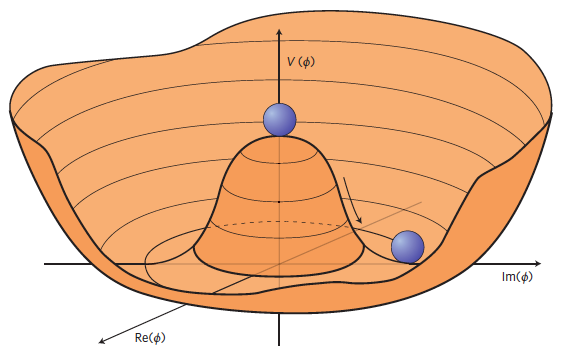
\includegraphics[width=\linewidth]{figures/theory_chapter/higgspotential.png}
\caption{The "wine bottle" Higgs potential hill, from reference \cite{EllisHiggs}}
\label{fig:potential}
\end{figure}

When the ball is balanced at the top of the potential "hill", the configuration is spatially symmetric: that is, no direction is privileged over any other. However, when this delicate balance is even slightly disturbed, the ball will roll down the hill in some direction, resulting in a final state that is $\emph{not}$ symmetrical. This is the phenomenon known as "spontaneous symmetry breaking".

Using the language of quantum field theory, we can add spontaneously-breakable symmetric potential terms to a Lagrangian. If we do so, the phenomenon of symmetry breaking allows us to rewrite these terms as a combination of massless fields (one for each "choice" the symmetry breaking must make) and massive fields (corresponding to the leftover degrees of freedom). If we rewrite the "wine-bottle" potential in this way, for example, the one new massless field corresponds to the ball's angular position along the circle at the base, while the massive field corresponds to the ball's  radial position "up" or "down" the hill. The massless particles that arise from these massless fields are known as Goldstone bosons.

We are now ready to discuss the Higgs mechanism. We can combine the electromagnetic and weak nuclear forces as different manifestations of the same force, called the electroweak force, that transforms like $U(1) \times SU(2)$. We write the terms of the Standard Model electroweak Lagrangian, noting that, since the weak interaction is observed to be chiral, it couples differently to left- and right-handed fermions.

In this case, the generator of the U(1) symmetry ($\alpha(x)$) is not the electric charge $Q$ as in our previous example, but is instead the "Weak Hypercharge" $Y = 2(Q -I_{3})$, where $I_{3}$ is the third component of the "Weak Isospin" $I$. For right-handed particles, $I_{3} = 0$, for left-handed up/charm/top quarks and neutrinos, $I_{3} = +\frac{1}{2}$, and for left-handed down/strange/bottom quarks and charged leptons, $I_{3} = +\frac{1}{2}$. We will call our U(1) boson $B_{\mu}$ rather than $A_{\mu}$, to distinguish it from the photon. For a fermion $\psi$ (u/c/s/e/$\mu$/$\tau$) that couples weakly to another fermion $\psi'$, we can write the left-and-right-handed components of f as 

$L = \begin{pmatrix} \psi_{L} \\ \psi'_{L} \end{pmatrix}$, $R = \begin{pmatrix}\psi_{R} \end{pmatrix}$.

Similarly, the generators of the SU(2) symmetry are the three matrices $\tau_{i}$, one corresponding to each weak boson $W^{\mu}_{i}$. The self-interaction term for the weak interaction is $L_{kin} = -\frac{1}{4}G^{\mu \nu}G_{\mu \nu}$, where:

\begin{equation}
G_{\mu \nu} = \partial_{\mu} W_{\nu} - \partial_{\nu} W_{\mu}+\frac{g}{2} W_{\mu}\times W_{\nu}
\end{equation}

We can define a new covariant derivative capturing the weak interaction terms as well:

\begin{equation}
D^{\mu} = \partial^{\mu}- \frac{1}{2}iYg_{1}B^{\mu} -\frac{1}{2}i I g_2 \Sigma \tau_{i}W_{i}^\mu
\end{equation}

Thus, the full electroweak $SU(2)_L \times U(1)$ Lagrangian is:

\begin{equation}
\mathcal{L} = i\bar{R}\gamma^{\mu}D_{\mu}R + i\bar{L}\gamma^{\mu}D_{\mu}L -\frac{1}{4}G^{\mu \nu}G_{\mu \nu} -\frac{1}{4}F^{\mu \nu} F_{\mu \nu}
\end{equation}

However, we note that this Lagrangian does not allow for gauge boson mass or fermion mass, as a fermion mass term $m\bar{\psi}\psi = m(\bar{\psi_{R}}\psi_{L}+\bar{\psi_{L}}\psi_{R})$ is not an SU(2) singlet and would thus not be invariant under the SU(2) symmetry. 

To rectify this, we can introduce a new complex SU(2) doublet scalar field:
\begin{equation}
\phi = \begin{pmatrix} \phi^{+} \\ \phi^{0} \end{pmatrix} = \begin{pmatrix} \phi_{1} + i\phi_{2}  \\ \phi_{3} + i\phi_{4} \end{pmatrix}
\end{equation}

called the $\emph{Higgs field}$. It follows the Lagrangian

\begin{equation}
\mathcal{L} = T-V = (D^{\mu}\phi)^{\dag}(D_{\mu}\phi) - {\mu}^2\phi^{\dag}\phi - \lambda(\phi^{\dag}\phi)^{2}
\end{equation}

which, if $\mu^{2} < 0$ has a minimum at
\begin{equation}
\phi^{\dag}\phi = \frac{-\mu^{2}}{2 \lambda} = \frac{v^{2}}{2}
\end{equation}

We note that the potential is symmetric, so we can pick a direction to "break the symmetry" in. Let us define the vacuum as:

\begin{equation}
\phi_0 = \frac{1}{\sqrt{2}} \begin{pmatrix} 0 \\ v \end{pmatrix}
\end{equation}


Then, for any arbitrary configuration of the field, we can expand the potential about the minimum as

\begin{equation}
\phi(x) = \frac{1}{\sqrt{2}} \begin{pmatrix} 0 \\ (v + h(x)) \end{pmatrix}
\label{eq:min}
\end{equation}

We can expand the kinetic term in the Lagrangian as

\begin{equation}
(D^{\mu}\phi)^{\dag}(D_{\mu}\phi) = \frac{1}{2}(\partial_{\mu}h)(\partial^{\mu}h)+ \phi^{\dag}(\frac{1}{2}iYg_{1}B_{\mu} -\frac{1}{2}iI g_2 \Sigma \tau_{i}W_{i\mu})^{\dag}(\frac{1}{2}iYg_{1}B^{\mu} -\frac{1}{2}iI g_2 \Sigma \tau_{i}W_{i}^{\mu}) \phi
\end{equation} 

Which, using the definitions of the three tau matrices, and putting Y = I = 1, becomes

\begin{align}
  \begin{aligned}
\frac{1}{2}(\partial_{\mu}h)(\partial^{\mu}h) + \frac{1}{8} |\begin{bmatrix} g_{1}B_{\mu}+g_{2}W_{\mu}^{3} & g_{2}(W_{\mu}^{1}-iW_{\mu}^{2}) \\ g_{2}(W_{\mu}^{1}+iW_{\mu}^{2}) & g_{1}B_{\mu}+g_{2}W_{\mu}^{3} \end{bmatrix} \begin{bmatrix} 0 \\ v \end{bmatrix}|^{2} \\
= \frac{1}{2}(\partial_{\mu}h)(\partial^{\mu}h) + \frac{1}{8}v^{2}g_{2}^{2}((W_{\mu}^{1})^{2}+(W_{\mu}^{2})^{2})) + \frac{1}{8}v^{2}(g_{1} B{\mu}-g_{2}W_{\mu}^{3})^{2}
  \end{aligned}&&&
\end{align}

If we again define some new field combinations here:

\begin{align}
  \begin{aligned}
{W_{\mu}^{+} -\frac{1}{\sqrt{2}}(W_{\mu}^{1}-iW_{\mu}^{2})}\\
{W_{\mu}^{-} -\frac{1}{\sqrt{2}}(W_{\mu}^{1}+iW_{\mu}^{2})}\\
{Z_{\mu} = \frac{g_{1}B{\mu}+g_{2}W_{\mu}}{\sqrt{{g_1}^2+{g_2}^2}}}\\ 
{A_{\mu} = \frac{g_{1}B{\mu}-g_{2}W_{\mu}}{\sqrt{{g_1}^2+{g_2}^2}}}
  \end{aligned}&&&
\end{align}

then we get: 

\begin{equation}
\frac{1}{2}(\partial_{\mu}h)(\partial^{\mu}h) + (\frac{1}{2}vg_{2})^{2}W_\mu^{+}W_\mu^{-}+(\frac{1}{2}v(\sqrt{{g_1}^2+{g_2}^2}))^{2}Z_{\mu}
\end{equation}

And we see that Z field and the two W fields have acquired mass terms, while the A field has remained massless. This corresponds to what we observe in the real world: the W bosons and the Z boson are massive, while the photon remains massless!

For fermions, the coupling to the Higgs field looks like (for some constant $g_{f}$):

\begin{equation}
g_{f}(\bar{f}_{L}\phi f_{R} + \phi^{\dag}\bar{f}_{R} f_{L})
\end{equation}


We note that, if we expand $\phi(x)$ about the minimum as in \ref{eq:min}, we find that the coupling term now looks like:

\begin{equation}
\frac{g_{f}v}{\sqrt{2}}(\bar{f}_{L}f_{R} + \bar{f}_{R}f_{L}) + \frac{g_{f}}{\sqrt{2}}(\bar{f}_{L}f_{R} + \bar{f}_{R}f_{L})
\end{equation}


Thus, the presence of the Higgs field allows us to have fermion mass terms in our Lagrangians, where the masses are $m_{f} = \frac{g_{f}v}{\sqrt{2}}$. However, we note that, at the current time, there is no way to derive the $g_{f}$ coupling theoretically: thus, while the Higgs mechanism now allows us to have massive fermions in our theory, it does not actually determine what the masses of these fermions are.

Finally, we note that if we expand the potential term in the complex Klein-Gordon Lagrangian for the Higgs field about the minimum, that is, 

\begin{align}
  \begin{aligned}
V = {\mu}^2\phi^{\dag}\phi + \lambda(\phi^{\dag}\phi)^{2} = \frac{1}{2}{\mu}^2(v+h)^{2} + \frac{1}{4}\lambda(v+h)^{4} \\
= -\frac{1}{2}{\lambda v^{2}}(v+h)^{2} + \frac{1}{4}\lambda(v+h)^{4} \\
= -\frac{1}{2}\lambda(v^{4} + 2v^{3}h + v^{2}h^{2}) + \frac{1}{4}\lambda(v^{4}+4vh^{3}+6v^{2}h^{2} + 4v^{3}h + h^{4})
  \end{aligned}&&&
\end{align}

we see a mass term of the form

\begin{equation}
(\frac{M_{h}^{2}}{2})h^{2} = \frac{6}{4}\lambda v^{2} h^{2} - \frac{1}{2}\lambda v^{2} h^{2} = \lambda v^{2} h^{2}
\end{equation}

That is, $M_{h} = v \sqrt{2 \lambda}$.

In sum: without a Higgs field, in order for the Standard Model electroweak Lagrangian to preserve $SU(2)_L \times U(1)$ symmetry, we are forbidden from including mass terms for the fermions or the gauge bosons. However, by adding this additional field to the model and breaking its symmetry, we find that we can include fermion mass terms that do not violate the $SU(2)_L \times U(1)$ symmetry, and that the electroweak gauge bosons now acquire mass terms by default. Furthermore, this new field also has a mass. This is a remarkable result: by adding one extra field to the model, we have solved several different problems in one fell swoop!

\section{The Higgs Boson and Its Couplings} \label{sec:Higgs Couplings} 

As we have seen, the Standard Model Higgs is massive, and couples directly to all other massive particles (with the possible exception of neutrinos; this is an active area of research). However, the existence of the Higgs is clearly not all there is to the story: the Standard Model is noticeably incomplete (What are dark matter and dark energy? What determines the exact masses of each of the fermions? Why have we never observed right-handed neutrinos? Can we unify other forces like we have unified electromagnetism and the weak force?). In the majority of proposed Beyond-the-Standard Model extensions, other particles that would interact with the Standard Model Higgs are introduced, including additional Higgs fields, as well as new massive fermions and bosons.

With the discovery of the Higgs, it can be argued that we have now entered an era of precision-measurement in collider physics. By closely studying interactions that are very sensitive to the injection of new physics, we can potentially detect deviations from the Standard Model: in many cases, we may see hints of the existence of new particles through changes to quantities of interest well before we are actually able to produce these particles in colliders directly. Due to the Higgs coupling to all massive particles, Higgs interactions are especially sensitive to new physics, and thus can serve as a useful bellwether for physics beyond the standard model.

The Large Hadron Collider is a proton-proton collider; as such, physics processes that occur in it are almost always initiated by quarks or gluons. The predominant production modes are, in order of frequency, gluon-gluon fusion ($ggF$), vector boson fusion ($VBF$), vector-boson associated ($VH$) and top-associated ($ttH$). The top-associated Higgs production mode is of particular interest to many experimentalists due to its direct dependence on the Higgs coupling to a fermion- by closely measuring the frequency and properties of the $ttH$ mode, we can better understand the nature of this variety of couplings. Rarer production modes, such as single-top associated Higgs production ($tH$), can shed still more light on the nature of the top-quark/Higgs coupling (called the top quark Yukawa coupling), but are much more difficult to observe. The $tH$ process occurs in two final-state modes, $tWH$ and $tHj$; however, there is some nuance in their definitions which we will come to shortly.

\begin{figure}[htp]
  \centering
         \begin{subfigure}[b]{0.5\textwidth}
         \centering
         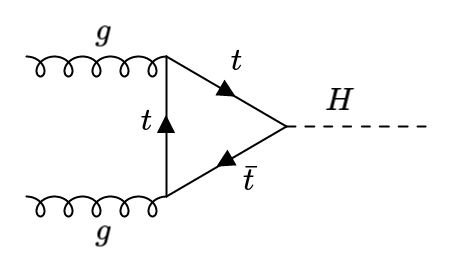
\includegraphics[width=\textwidth,valign=m]{figures/theory_chapter/ggF.png}
         \caption{ggF}
         \label{fig:ggF}
     \end{subfigure}
     \hfill
       \begin{subfigure}[b]{0.3\textwidth}
         \centering
         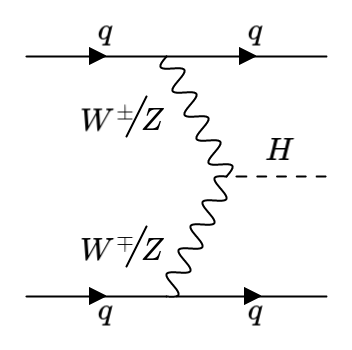
\includegraphics[width=\textwidth,valign=m]{figures/theory_chapter/VBF.png}
         \caption{VBF}
         \label{fig:VBF}
     \end{subfigure}
     \hfill 
     \\
         \centering
         \begin{subfigure}[b]{0.5\textwidth}
         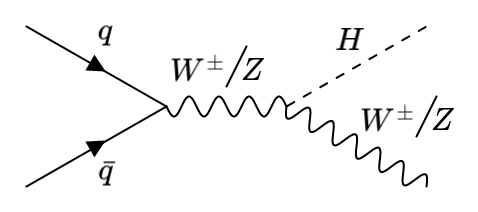
\includegraphics[width=\textwidth]{figures/theory_chapter/VH.png}
         \caption{VH}
         \label{fig:VH}
     \end{subfigure}
  \label{fig:Higgsmodes}
  \caption{Feynman diagrams depicting the three leading Higgs production modes. Made with \cite{FeynmanMaker}}  
\end{figure}

\begin{figure}[htp]
  \centering
       \begin{subfigure}[b]{0.3\textwidth}
         \centering
         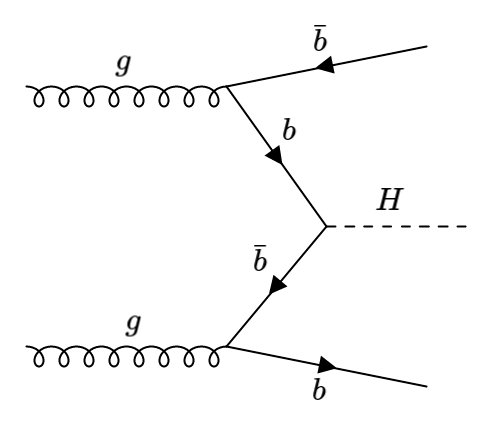
\includegraphics[width=\textwidth,valign=m]{figures/theory_chapter/bbH.png}
         \caption{bbH}
         \label{fig:bbH}
     \end{subfigure}
     \hfill
         \begin{subfigure}[b]{0.3\textwidth}
         \centering
         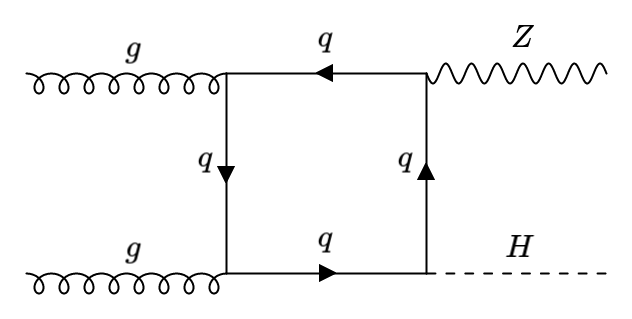
\includegraphics[width=\textwidth,valign=m]{figures/theory_chapter/ggZH.png}
         \caption{gg $\rightarrow ZH$ }
         \label{fig:ggZH}
     \end{subfigure}
     \hfill
         \begin{subfigure}[b]{0.3\textwidth}
         \centering
         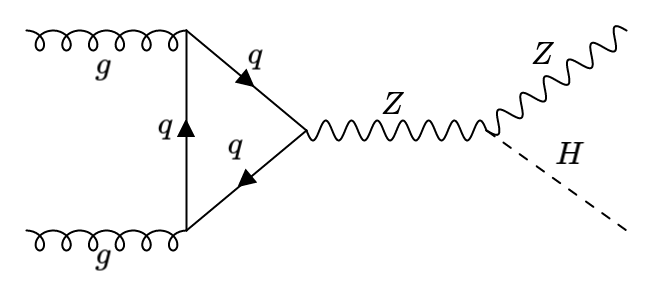
\includegraphics[width=\textwidth,valign=m]{figures/theory_chapter/ggZH2.png}
         \caption{Additional gg $\rightarrow ZH$ }
         \label{fig:ggZH}
     \end{subfigure}
     \hfill
  \label{fig:loopmodes}
  \caption{Feynman diagrams depicting relevant less-common Higgs production modes.Made with \cite{FeynmanMaker}}  
\end{figure}

\begin{figure}[htp]
  \centering
       \begin{subfigure}[b]{0.3\textwidth}
         \centering
         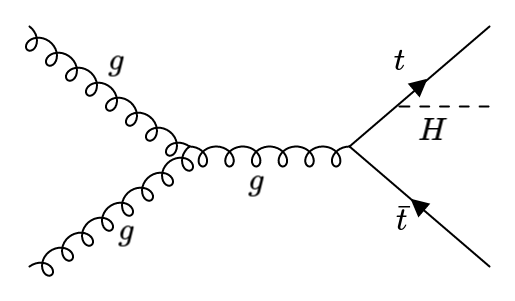
\includegraphics[width=\textwidth]{figures/theory_chapter/ttH1.png}
         \label{fig:ttH1}
     \end{subfigure}
     \hfill
       \begin{subfigure}[b]{0.3\textwidth}
         \centering
         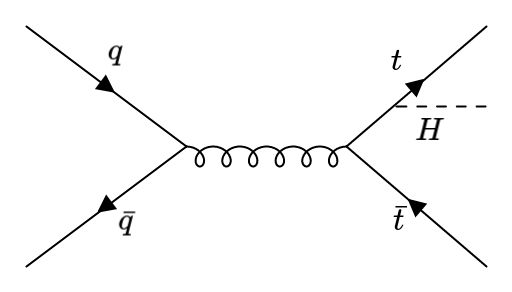
\includegraphics[width=\textwidth]{figures/theory_chapter/ttH2.png}
         \label{fig:ttH2}
     \end{subfigure}
     \hfill
       \begin{subfigure}[b]{0.3\textwidth}
         \centering
         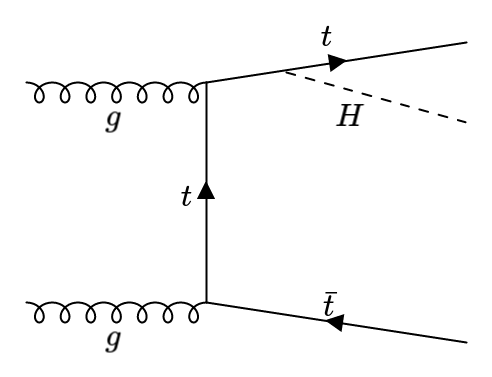
\includegraphics[width=\textwidth]{figures/theory_chapter/ttH3.png}
         \label{fig:ttH3}
     \end{subfigure}
     \hfill
         \begin{subfigure}[b]{0.3\textwidth}
         \centering
         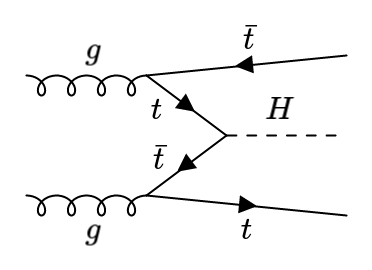
\includegraphics[width=\textwidth]{figures/theory_chapter/ttH4.png}
         \label{fig:ttH4}
     \end{subfigure}
     \hfill 
  \label{fig:loopmodes}
  \caption{Feynman diagrams depicting ttH production modes.Made with \cite{FeynmanMaker}}  
\end{figure}

\begin{figure}[htp]
  \centering
       \begin{subfigure}[b]{0.3\textwidth}
         \centering
         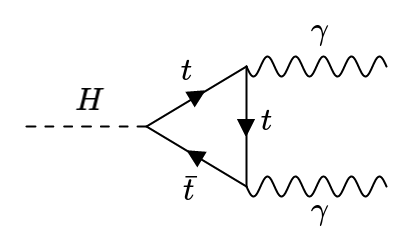
\includegraphics[width=\textwidth,valign=m]{figures/theory_chapter/toploop.png}
         \caption{Top-mediated}
         \label{fig:toploop}
     \end{subfigure}
     \hfill
         \begin{subfigure}[b]{0.4\textwidth}
         \centering
         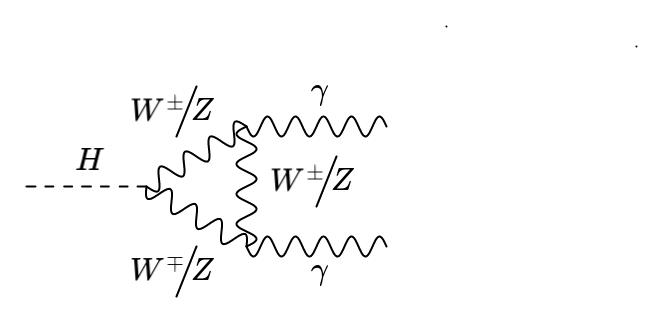
\includegraphics[width=\textwidth,valign=m]{figures/theory_chapter/Wloop1.png}
         \caption{W $\rightarrow \gamma$ }
         \label{fig:Wloop1}
     \end{subfigure}
     \hfill 
        \begin{subfigure}[b]{0.3\textwidth}
         \centering
         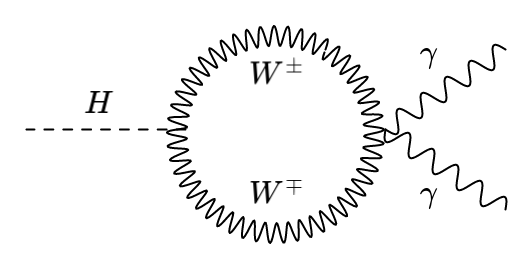
\includegraphics[width=\textwidth,valign=m]{figures/theory_chapter/Wloop2.png}
         \caption{W $\rightarrow \gamma \gamma$}
         \label{fig:Wloop2}
     \end{subfigure}
     \hfill
  \label{fig:loopmodes}
  \caption{Feynman diagrams depicting the leading-order processes contributing to the Higgs diphoton decay. Made with \cite{FeynmanMaker}}  
\end{figure}

Similarly, the dominant decay mode of the Higgs is to bottom quarks ($H \rightarrow bb$), followed by to W bosons ($H \rightarrow WW$), gluons ($H \rightarrow WW$), tau leptons ($H \rightarrow \tau \tau$), charm quarks ($H \rightarrow bb$), Z bosons ($H \rightarrow ZZ$), photons ($H \rightarrow \gamma \gamma$), and a Z boson and a photon ($H \rightarrow Z \gamma$). Because the Higgs does not couple to massless particles directly, the decays to gg and $\gamma \gamma$ are mediated by loop diagrams, most often involving top quarks.

Investigating each of these decay modes has different benefits and detriments. While the Higgs decay to bottom quarks is the most common, correctly identifying and accurately reconstructing quarks and gluons using the jets that they produce in detectors is often very difficult. Decays to W bosons, Z bosons, and $\tau$ leptons provide "cleaner" channels, but because the W, Z and $\tau$ decay dominantly to hadrons, similar reconstruction issues occur unless we restrict ourselves to the rarer leptonic subchannels of these decays. The Higgs to diphoton channel occurs very rarely, but offers a much more unambiguous signal, as the odds of misidentifying high-energy gamma rays are fairly low.

Additionally, we must consider combinatorics: in the ttH production mode, for instance, the final state contains two bottom quarks from the decay of the associated top quarks. If we choose to examine the subchannel in which the Higgs decays to bottom quarks as well, we find that we have at least four final-state bottom quark jets in the event, with 12 different unique assignments of bottom quark jets to parent particles. Correctly matching up which jet originated from which parent particle thus further complicates the reconstruction problem.

The rate of a particular physics production mode or scattering process is parameterized using a quantity called the cross-section $\sigma$, which is measured in units of "barns". Similarly, the rate of a particular decay process is parameterized using a quantity called the decay width $\Gamma$, which measures the probability of a particular decay occurring per unit time. We can also define the "Branching Fraction" of a particular process: if $\Gamma_{H}$ denotes the sum of all Higgs decay widths, for a given process $H \rightarrow XX$ we define

\begin{equation}
Br(H \rightarrow XX) = \frac{\Gamma(H \rightarrow XX)}{\Gamma_{H}}
\end{equation}

The second of the two analyses discussed in this dissertation is a survey of a wide variety of Higgs-based physics processes using the Higgs-to-diphoton decay channel (referred to in this dissertation as the "Higgs Couplings Analysis"). A combined fit is performed in different regions of phase space that correspond to the $ggF$, $VBF$, $VH$, $ttH$, and $tH$ processes; by doing this, we can extract limits on the individual Higgs production cross-sections in targeted regions of phase space.

\begin{figure}
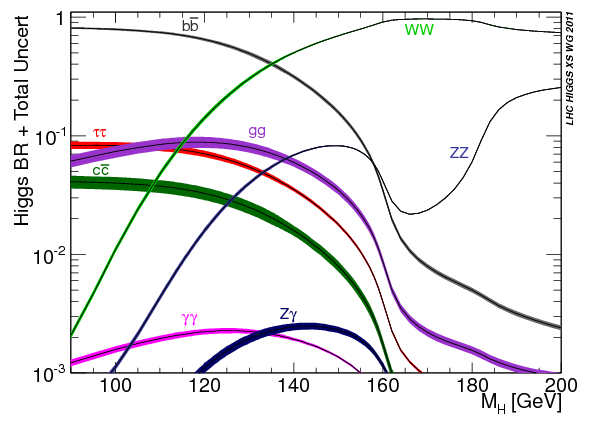
\includegraphics[width=\linewidth]{figures/theory_chapter/HiggsBR.png}
\caption{The branching ratio of the Higgs to various final state particles as a function of its mass (now known to be ~125 GeV), from reference \cite{YellowReport1}.}
\end{figure}

\begin{table}[h]
    \centering
    \begin{tabular}{cc}
        	Decay Mode & Branching fraction [\%] \\
            $H \rightarrow bb $ & $ 57.5 \pm 1.9 $ \\
			$H \rightarrow WW $ & $ 21.6 \pm 0.9 $ \\
			$H \rightarrow gg $ & $ 8.56 \pm 0.86 $ \\
			$H \rightarrow \tau \tau $ & $ 6.30 \pm 0.36 $ \\
			$H \rightarrow cc $ & $ 2.90 \pm 0.35 $ \\
			$H \rightarrow ZZ $ & $ 2.67 \pm 0.11 $ \\
			$H \rightarrow \gamma \gamma $ & $ 0.228 \pm 0.011 $ \\
			$H \rightarrow Z \gamma $ & $ 0.155 \pm 0.014 $ \\
			$H \rightarrow \mu \mu $ & $ 0.022 \pm 0.001 $ \\
    \end{tabular}
    \caption{Higgs decay modes and branching fractions, for a Standard Model Higgs with mass of 125.09 GeV \cite{YellowReport4}}
    \label{mytable}
\end{table}

Cross-sections are calculated at a given perturbation-theoretic "order", indicating how many additional correction terms (often indicated by Feynman diagrams with internal loops and vertices) are accounted for in the calculation- for a given process, leading-order (or "LO"), next-to-leading order ("NLO"), and next-to-next-to-leading order ("NNLO") indicate increasing numbers of correction terms. Calculating and simulating to higher orders is more accurate, but is often much more computationally expensive. These correction terms can be applied for both electroweak (EW) and quantum-chromodynamical (QCD) effects.

In addition to considering which corrections to apply, we must also consider the flavor scheme of the Monte Carlo generator. Physics processes can be initiated by real quarks or gluons that are present in the initial scattering protons, as well as virtual quarks that are present in the primordial soup of energy that binds each proton together. In the five-flavor Parton Distribution Function (PDF) scheme, we consider massless virtual bottom quarks to be constituents of the proton that are capable of initiating physics processes, while in the four-flavor PDF scheme, we do not. These schemes differ primarily in which diagrams they treat as corrections and which they do not- thus, if we perform QCD corrections at all orders (that is, NN...NNLO), we find that these two schemes produce identical results \cite{FedericotH}. Diagrams from the five-flavor PDF scheme that are initiated by a bottom quark can be mapped into the four-flavor scheme by adding an additional bottom-quark to the final state; however, for $ttH$, $tt\gamma\gamma$ and $tWH$ processes, this presents a number of nontrivial modelling issues \cite{FedericotWH}. While the five-flavor scheme offers easier calculation and the ability to model more processes, the four-flavor scheme is better at modelling Higgs kinematics, such as $p_{T}$ and bottom-quark  $p_{T}$. For these reasons, we use the four-flavor scheme to model the $tHj$ process only (henceforth called $tHjb$ due to the presence of the additional final-state b-jet) and the five-flavor scheme for all other top-quark-based processes. 

\begin{figure}[htp]
  \centering
       \begin{subfigure}[b]{0.3\textwidth}
         \centering
         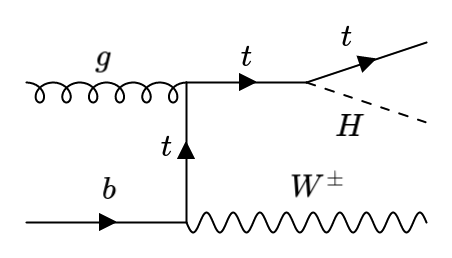
\includegraphics[width=\textwidth]{figures/theory_chapter/tWH1.png}
         \caption{A tWH mode}
         \label{fig:tWH1}
     \end{subfigure}
     \hfill
         \begin{subfigure}[b]{0.3\textwidth}
         \centering
         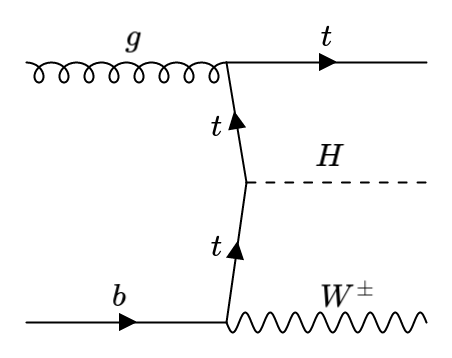
\includegraphics[width=\textwidth]{figures/theory_chapter/tWH2.png}
         \caption{A tWH mode}
         \label{fig:tWH2}
     \end{subfigure}
     \hfill
         \begin{subfigure}[b]{0.3\textwidth}
         \centering
         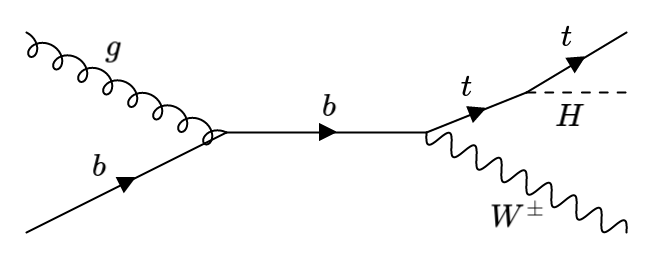
\includegraphics[width=\textwidth]{figures/theory_chapter/tWH3.png}
         \caption{A tWH mode}
         \label{fig:tWH3}
     \end{subfigure}
     \hfill
         \begin{subfigure}[b]{0.3\textwidth}
         \centering
         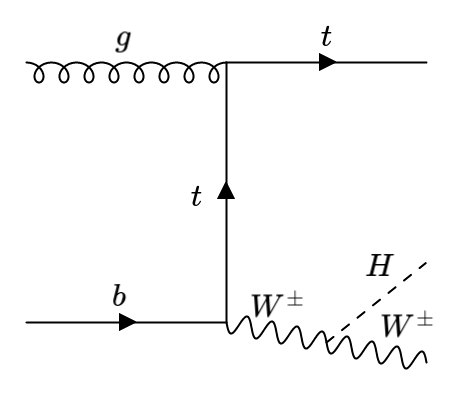
\includegraphics[width=\textwidth]{figures/theory_chapter/tWH4.png}
         \caption{A tWH mode}
         \label{fig:tWH4}
     \end{subfigure}
     \hfill
         \begin{subfigure}[b]{0.3\textwidth}
         \centering
         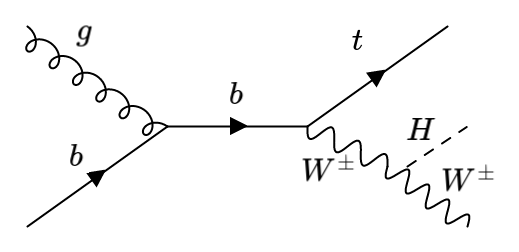
\includegraphics[width=\textwidth]{figures/theory_chapter/tWH5.png}
         \caption{A tWH mode}
         \label{fig:tWH5}
     \end{subfigure}
  \label{fig:tWHmodes}
  \caption{Feynman diagrams depicting the leading-order terms for $tWH$. Because all diagrams contain initial b-quarks, all of these processes can only occur in the five-flavor PDF scheme. Made with \cite{FeynmanMaker}}  
\end{figure}

\begin{figure}[htp]
  \centering
       \begin{subfigure}[b]{0.3\textwidth}
         \centering
         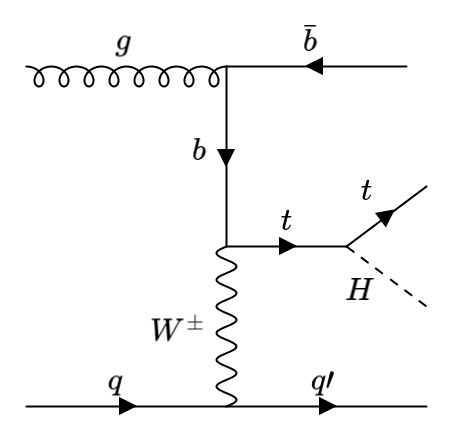
\includegraphics[width=\textwidth]{figures/theory_chapter/tHjb1.png}
         \caption{A tHjb mode}
         \label{fig:tHjb1}
     \end{subfigure}
     \hfill
         \begin{subfigure}[b]{0.3\textwidth}
         \centering
         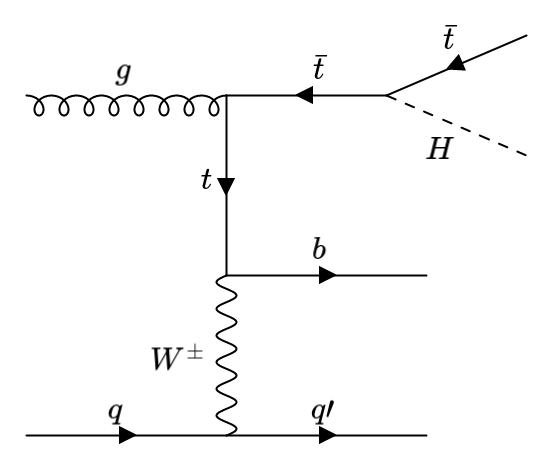
\includegraphics[width=\textwidth]{figures/theory_chapter/tHjb2.png}
         \caption{A tHjb mode}
         \label{fig:tHjb2}
     \end{subfigure}
     \hfill
         \begin{subfigure}[b]{0.3\textwidth}
         \centering
         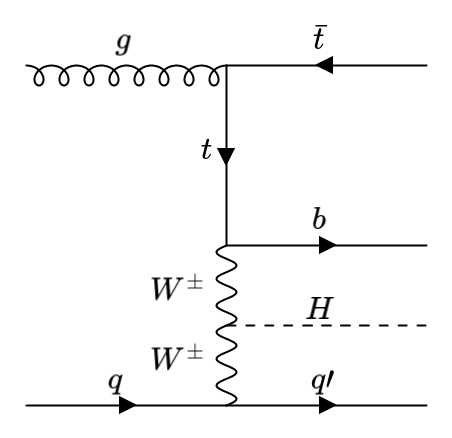
\includegraphics[width=\textwidth]{figures/theory_chapter/tHjb3.png}
         \caption{A tHjb mode}
         \label{fig:tHjb3}
     \end{subfigure}
     \hfill
         \begin{subfigure}[b]{0.3\textwidth}
         \centering
         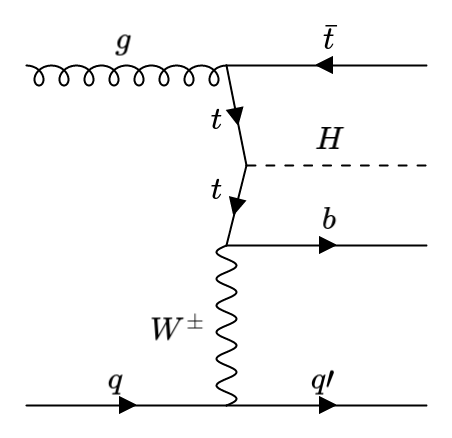
\includegraphics[width=\textwidth]{figures/theory_chapter/tHjb4.png}
         \caption{A tHjb mode}
         \label{fig:tHjb4}
     \end{subfigure}
     \hfill
         \begin{subfigure}[b]{0.3\textwidth}
         \centering
         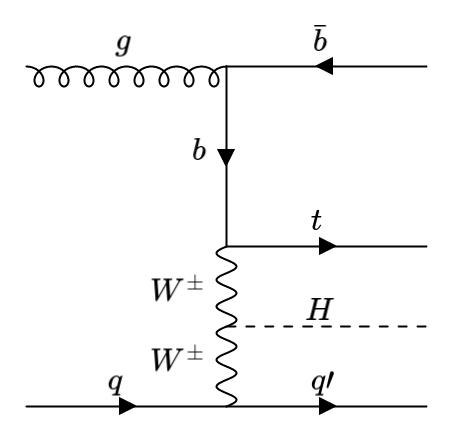
\includegraphics[width=\textwidth]{figures/theory_chapter/tHjb5.png}
         \caption{A tHjb mode}
         \label{fig:tHjb5}
     \end{subfigure}
  \label{fig:tHjbmodes}
  \caption{Feynman diagrams depicting the leading-order terms for $tHjb$, made with \cite{FeynmanMaker}. These diagrams are calculated using the four-flavor PDF scheme. Note that additional diagrams can be created by reversing the direction of the upper fermion "circuit" (the final-state top and bottom must be opposite sign, but $tHj\bar{b}$ and $\bar{t}Hjb$ are equally likely to occur).}  
\end{figure}


\subsection{CP-Violation in the Top Yukawa Coupling} \label{sec:CP-yukawa}


According to the Standard Model, the Higgs boson is a CP-even scalar boson: it is predicted to have spin-zero, with all its interactions CP-even. Previous analyses from both ATLAS and CMS have placed limits on the existence of anomalous CP-violating Higgs couplings to the gauge bosons (\cite{Aad_2016} \cite{Khachatryan_2016} and \cite{Sirunyan_2019}); however, any such couplings would be suppressed by a factor of 1/$(\Lambda)^2$ (where $\Lambda$ indicates the energy scale of the new CP-violating physics) \cite{Zhang_2011}, so these studies are thus somewhat limited in their sensitivity. Similarly, indirect measurements of the CP-nature of the Higgs coupling to fermions in loop-diagram mediated processes have been performed \cite{Ellis} \cite{Brod_2013}; however, these measurements are highly dependent on the choice of BSM model that induces CP violation.

The first of the two analyses detailed in this dissertation, referred to as the "ttHCP Analysis", marks the first direct measurement of the CP-nature of the Higgs couplings to fermions. Because the top quark Yukawa is the strongest Higgs coupling, it is one of the most useful channels for the performance of this measurement. A CP-violating top Yukawa coupling will influence production rates and kinematics in top-pair associated Higgs production ($t \bar{t} H$) and single-top associated Higgs production ($tH$, specifically $tHjb$ and $tWH$). Additionally, CP-violation in the top Yukawa coupling will modify the rates of gluon-gluon fusion Higgs production and Higgs to diphoton decay; however, because these two processes are loop-mediated, they are sensitive to other forms of new physics as well, and thus not enough to directly constrain the CP nature of the top Yukawa coupling on their own. Previous ATLAS analyses have measured the CP properties of the top Yukawa coupling in this manner, but such constraints are indirect \cite{Aaboud_2018} \cite{couplings80fb}.

Because of its combined direct and indirect sensitivity to the top Yukawa coupling, we thus find that the $ttH$ and $tH$ processes with $H \rightarrow \gamma \gamma $ provide a well-motivated channel for probing the CP-structure of the top-Higgs interaction. In addition, the presence of two photons in the event final state provides a clean signal, further motivating the use of this channel. 

Using the Higgs Characterization (HC) model \cite{HC}, we can parameterize the top-Higgs interaction in the presence of CP-violation as:

\begin{equation}
\mathcal{L} = -\frac{m_{t}}{v} \kappa_{t} \bar{t} (cos(\alpha)+ sin(\alpha) i \gamma^{5} )th
\end{equation}

for mixing angle $\alpha \in (-180^{\circ}, 180^{\circ})$ and $\kappa_{t} >= 0$.

With the coupling formulated in such a way, the $ttH$ cross-section can be parameterized as

\begin{equation}
\sigma_{ttH} =  A\kappa_{t}^{2} (cos(\alpha)^{2}) + B\kappa_{t}^{2} (sin(\alpha)^{2}) + E \kappa_{t}^{2} cos(\alpha)sin(\alpha)
\end{equation}

for some constants A, B, and E (with E expected to be zero for $ttH$), while the $tWH$ and $tHjb$ cross-sections can be parameterized as:

\begin{equation}
\sigma_{tH} =  A\kappa_{t}^{2} (cos(\alpha)^{2}) + B\kappa_{t}^{2} (sin(\alpha)^{2}) + C\kappa_{t} (cos(\alpha))+ D\kappa_{t} (sin(\alpha)) + E \kappa_{t}^{2} cos(\alpha)sin(\alpha) + F
\end{equation}

The C and D terms originate from destructive interference: because the $tH$ process contains diagrams where the Higgs couples to the top as well as diagrams where the Higgs couples to the W-boson, holding the W-Higgs coupling fixed while varying the top-Higgs coupling can alter the total cross-section of the process. Likewise, the F term indicates the contribution only from the diagrams that do not involve the top Yukawa coupling \cite{Maltoni_2001}. Furthermore, we note that the $ttH$ cross-section is the same for $\alpha = 0^{\circ}$ and $\alpha = 180^{\circ}$ while the $tH$ cross-section is not- thus, measuring the $tH$ interaction allows us to eliminate this degeneracy and determine the sign of the top Yukawa coupling.

Similarly, we can parameterize $\kappa_{g}$ and $\kappa_{\gamma}$ according to the parameterizations in \cite{Ellis}:

\begin{align}
\begin{aligned}
\kappa_{g}^{2} = 1.11\kappa_{t}^{2}cos(\alpha)^{2} + 2.6\kappa_{t}^{2}sin(\alpha)^{2} - 0.11\kappa_{t}cos(\alpha)\\ 
\kappa_{\gamma}^{2} = 0.08\kappa_{t}^{2}cos(\alpha)^{2} + 0.18\kappa_{t}^{2}sin(\alpha)^{2} - 0.72\kappa_{t}cos(\alpha) + 1.64
\end{aligned}
\end{align}

Cross-sections as a function of $\alpha$ as implemented in Monte Carlo simulation are given in \ref{tab:MCsamples_XS}. We note that, as $\alpha$ increases from $\alpha = 0^{\circ}$ (CP-even) to $\alpha = 90^{\circ}$ (CP-odd), the $ttH$ cross-section decreases while the $tH$ and $ggF$ cross-sections increase. Similarly, the $H \rightarrow \gamma \gamma$ branching ratio increases as $\alpha$ increases. Furthermore, introducing a CP-odd term changes the kinematics of the $ttH$ and $tH$ processes, and leads to events with different angular variable values (such as the angle between the two tops) as well as changing the energies and momenta of some decay products. By developing targeted analysis categories using these kinematic variables and parameterizing the yield in each category as a function of $\alpha$, we can thus perform a likelihood fit to the data and set limits on the true value of $\alpha$. 










\iffalse
In addition to the kappa-framework, the Couplings Analysis also makes use of an Effective Field Theory (EFT) approach to parameterize potential Higgs Couplings beyond the Standard Model. Effective Field Theories offer a model-independent way to parameterize new physics that may not be directly accessible at LHC energies. Using the Standard Model Effective Field Theory parameterization (SMEFT) \cite{SMEFT}, we can write the Lagrangian for new physics that exists at some energy scale $\Lambda >> v$ (where $v$ denotes the Higgs field vacuum expectation value of 246 GeV) as

\begin{equation}
\mathcal{L}_{SMEFT} = \mathcal{L}_{SM} + (\frac{v}{\Lambda})\mathcal{L}_{5} + (\frac{v}{\Lambda})^2 \mathcal{L}_{6}
\end{equation}

If we assume that lepton and baryon number are conserved, we find that we cannot have any $\mathcal{L}_{5}$ operators, as all allowable dimension-5 operators violate the conservation of lepton number; thus, the leading EFT terms are all proportional to $(\frac{v}{\Lambda})^2$ and have dimension-6.

The dimension-6 Lagrangian term can be expanded as a linear combination of all allowable dimension-6 operators:

\begin{equation}
\mathcal{L}_{6} = \sum_{i} c_{i}^6 O_{i}^{6}
\end{equation}

In the Couplings Analysis, the operators are chosen using the so-called "Warsaw Basis" \cite{Warsaw}; the $c_{i}$ terms are the free parameters to be determined by the final likelihood fit, called "Wilson Coefficients". A list of all allowed dimension-6 operators and their corresponding coefficients is given in \ref{tab:EFT}.

\begin{table}
  \centering
  \begin{tabular}{c l}
  \hline
  Wilson coefficient & Operator \\
  \hline
  $\cHbox$ & $(H^\dag H)\Box(H^\dag H)$\\
  $\cHDD$   & $\ \left(H^\dag D^\mu H\right)^* \left(H^\dag D_\mu H\right)$\\
  $\cHG$  & $H^\dag H\, G^A_{\mu\nu} G^{A\mu\nu}$  \\
  $\cHB$ &  $ H^\dag H\, B_{\mu\nu} B^{\mu\nu}$\\
  $\cHW$ &  $H^\dag H\, W^I_{\mu\nu} W^{I\mu\nu}$\\
  $\cHWB$ &  $ H^\dag \tau^I H\, W^I_{\mu\nu} B^{\mu\nu}$\\
  $\cHl1$ & $(H^\dag i\overleftrightarrow{D}_\mu H)(\bar l_p \gamma^\mu l_r)$\\
  $\cHl3$ & $(H^\dag i\overleftrightarrow{D}^I_\mu H)(\bar l_p \tau^I \gamma^\mu l_r)$\\
  $\cHe$  & $(H^\dag i\overleftrightarrow{D}_\mu H)(\bar e_p \gamma^\mu e_r)$\\
  $\cHq1$ & $(H^\dag i\overleftrightarrow{D}_\mu H)(\bar q_p \gamma^\mu q_r)$\\
  $\cHq3$ & $(H^\dag i\overleftrightarrow{D}^I_\mu H)(\bar q_p \tau^I \gamma^\mu q_r)$\\
  $\cHu$  & $(H^\dag i\overleftrightarrow{D}_\mu H)(\bar u_p \gamma^\mu u_r)$\\
  $\cHd$  & $(H^\dag i\overleftrightarrow{D}_\mu H)(\bar d_p \gamma^\mu d_r)$\\
  $\cuGAbs$ & $(\bar q_p \sigma^{\mu\nu} T^A u_r) \widetilde H \, G_{\mu\nu}^A$ \\
  $\cll1$   & $(\bar l_p \gamma_\mu l_r)(\bar l_s \gamma^\mu l_t)$ \\
  \hline
\end{tabular}
  \caption{Wilson coefficients $c_i$ and corresponding dimension-6 SMEFT operators $\mathcal{O}_i$ used in this analysis.}
  \label{tab:EFT}
\end{table}

Under this model, we can write the cross-section in some STXS bin as 

\begin{equation}
\sigma_{bin} =  \sigma_{bin}^{SM} + \sigma_{bin}^{interaction} + \sigma_{bin}^{BSM}
\end{equation}

where the first term refers to the Standard-Model cross-section, the second refers to the interaction between the SM and BSM physics processes, and the last refers to the BSM processes themselves.

We can also write:
\begin{equation}
\frac{\sigma_{bin}^{interaction}}{\sigma_{bin}^{SM}} = \sum_{i} A_{i} c_{i}
\frac{\sigma_{bin}^{BSM}}{\sigma_{bin}^{SM}} = \sum_{i} B_{ij} c_{i} c_{j}
\end{equation}

So we can parameterize the cross-section as:
\begin{equation}
\frac{\sigma_{bin}}{\sigma_{bin}^{SM}} = 1 + \sum_{i} A_{i} c_{i} + \sum_{i} B_{ij} c_{i} c_{j}
\end{equation}

Similarly, the Higgs partial decay width to diphotons (a measure of how often the Higgs decays to diphotons vs other channels) can be parameterized as follows:

\begin{equation}
\Gamma_{\gamma \gamma} = \Gamma_{\gamma \gamma}^{SM} + \Gamma_{\gamma \gamma}^{interaction} + \Gamma_{\gamma \gamma}^{BSM}
\Gamma_{\gamma \gamma} = 1 + \sum_{i} A_{i}^{\Gamma_{\gamma \gamma}} c_{i} + \sum_{i} B_{ij}^{\Gamma_{\gamma \gamma}} c_{i} c_{j}
\end{equation}

Combining these, we can parameterize the event yield in each STXS bin in terms of the Wilson coefficients, using Monte Carlo simulated events to determine the $A_{i}$ and $B_{ij}$ coefficients. This is detailed further in Section \ref{sec:CouplingsChapter}.
\fi
 

\chapter{The ATLAS Detector} \label{chap:detector_chapter}
	\section{The Large Hadron Collider} \label{sec:LHC} 

At roughly 27 kilometers in circumference, the Large Hadron Collider (LHC) at the Center for European Nuclear Research (CERN) is the largest machine ever built, slicing through the solid rock of the Jura mountains and running more than 100 meters beneath the Swiss-French border. It is a proton-proton collider operating at a center-of-mass energy of 13 TeV, circulating two beams of protons in opposite directions, each at more than 99\% the speed of light. By utilizing a system of radiofrequency (RF) cavities and dipole magnets, protons are delivered to four primary collision points in bunches spaced 25 nanoseconds apart \cite{LHCTDR}.

The LHC achieves such a powerful center-of-mass energy by repurposing a significant fraction of older collider physics infrastructure, including the Super Proton Synchrotron (SPS), which was itself one of the most powerful particle accelerators in the world at one time. In order to achieve collision, hydrogen atoms are first stripped of their electrons using an ionizing cathode filament in a device called a duoplasmatron; this produces a plasma that is filtered to produce beams of protons \cite{SPS}. The LINAC2, a linear accelerator, then accelerates the resultant proton beams to a collision energy of 50 MeV; the beams then move to the Proton Synchrotron Booster (PSB), a circular accelerator that accelerates them to an energy of 1.4 GeV, followed by the Proton Synchrotron (PS), a second circular accelerator that accelerates them to 25 GeV. Following this, beams enter the aforementioned Super Proton Synchrotron, where they are accelerated to a collision energy of 450 GeV before being injected into the Large Hadron Collider ring \cite{LHCTDR}. This infrastructure is depicted in Figure \ref{fig:LHC}.

\begin{figure}
  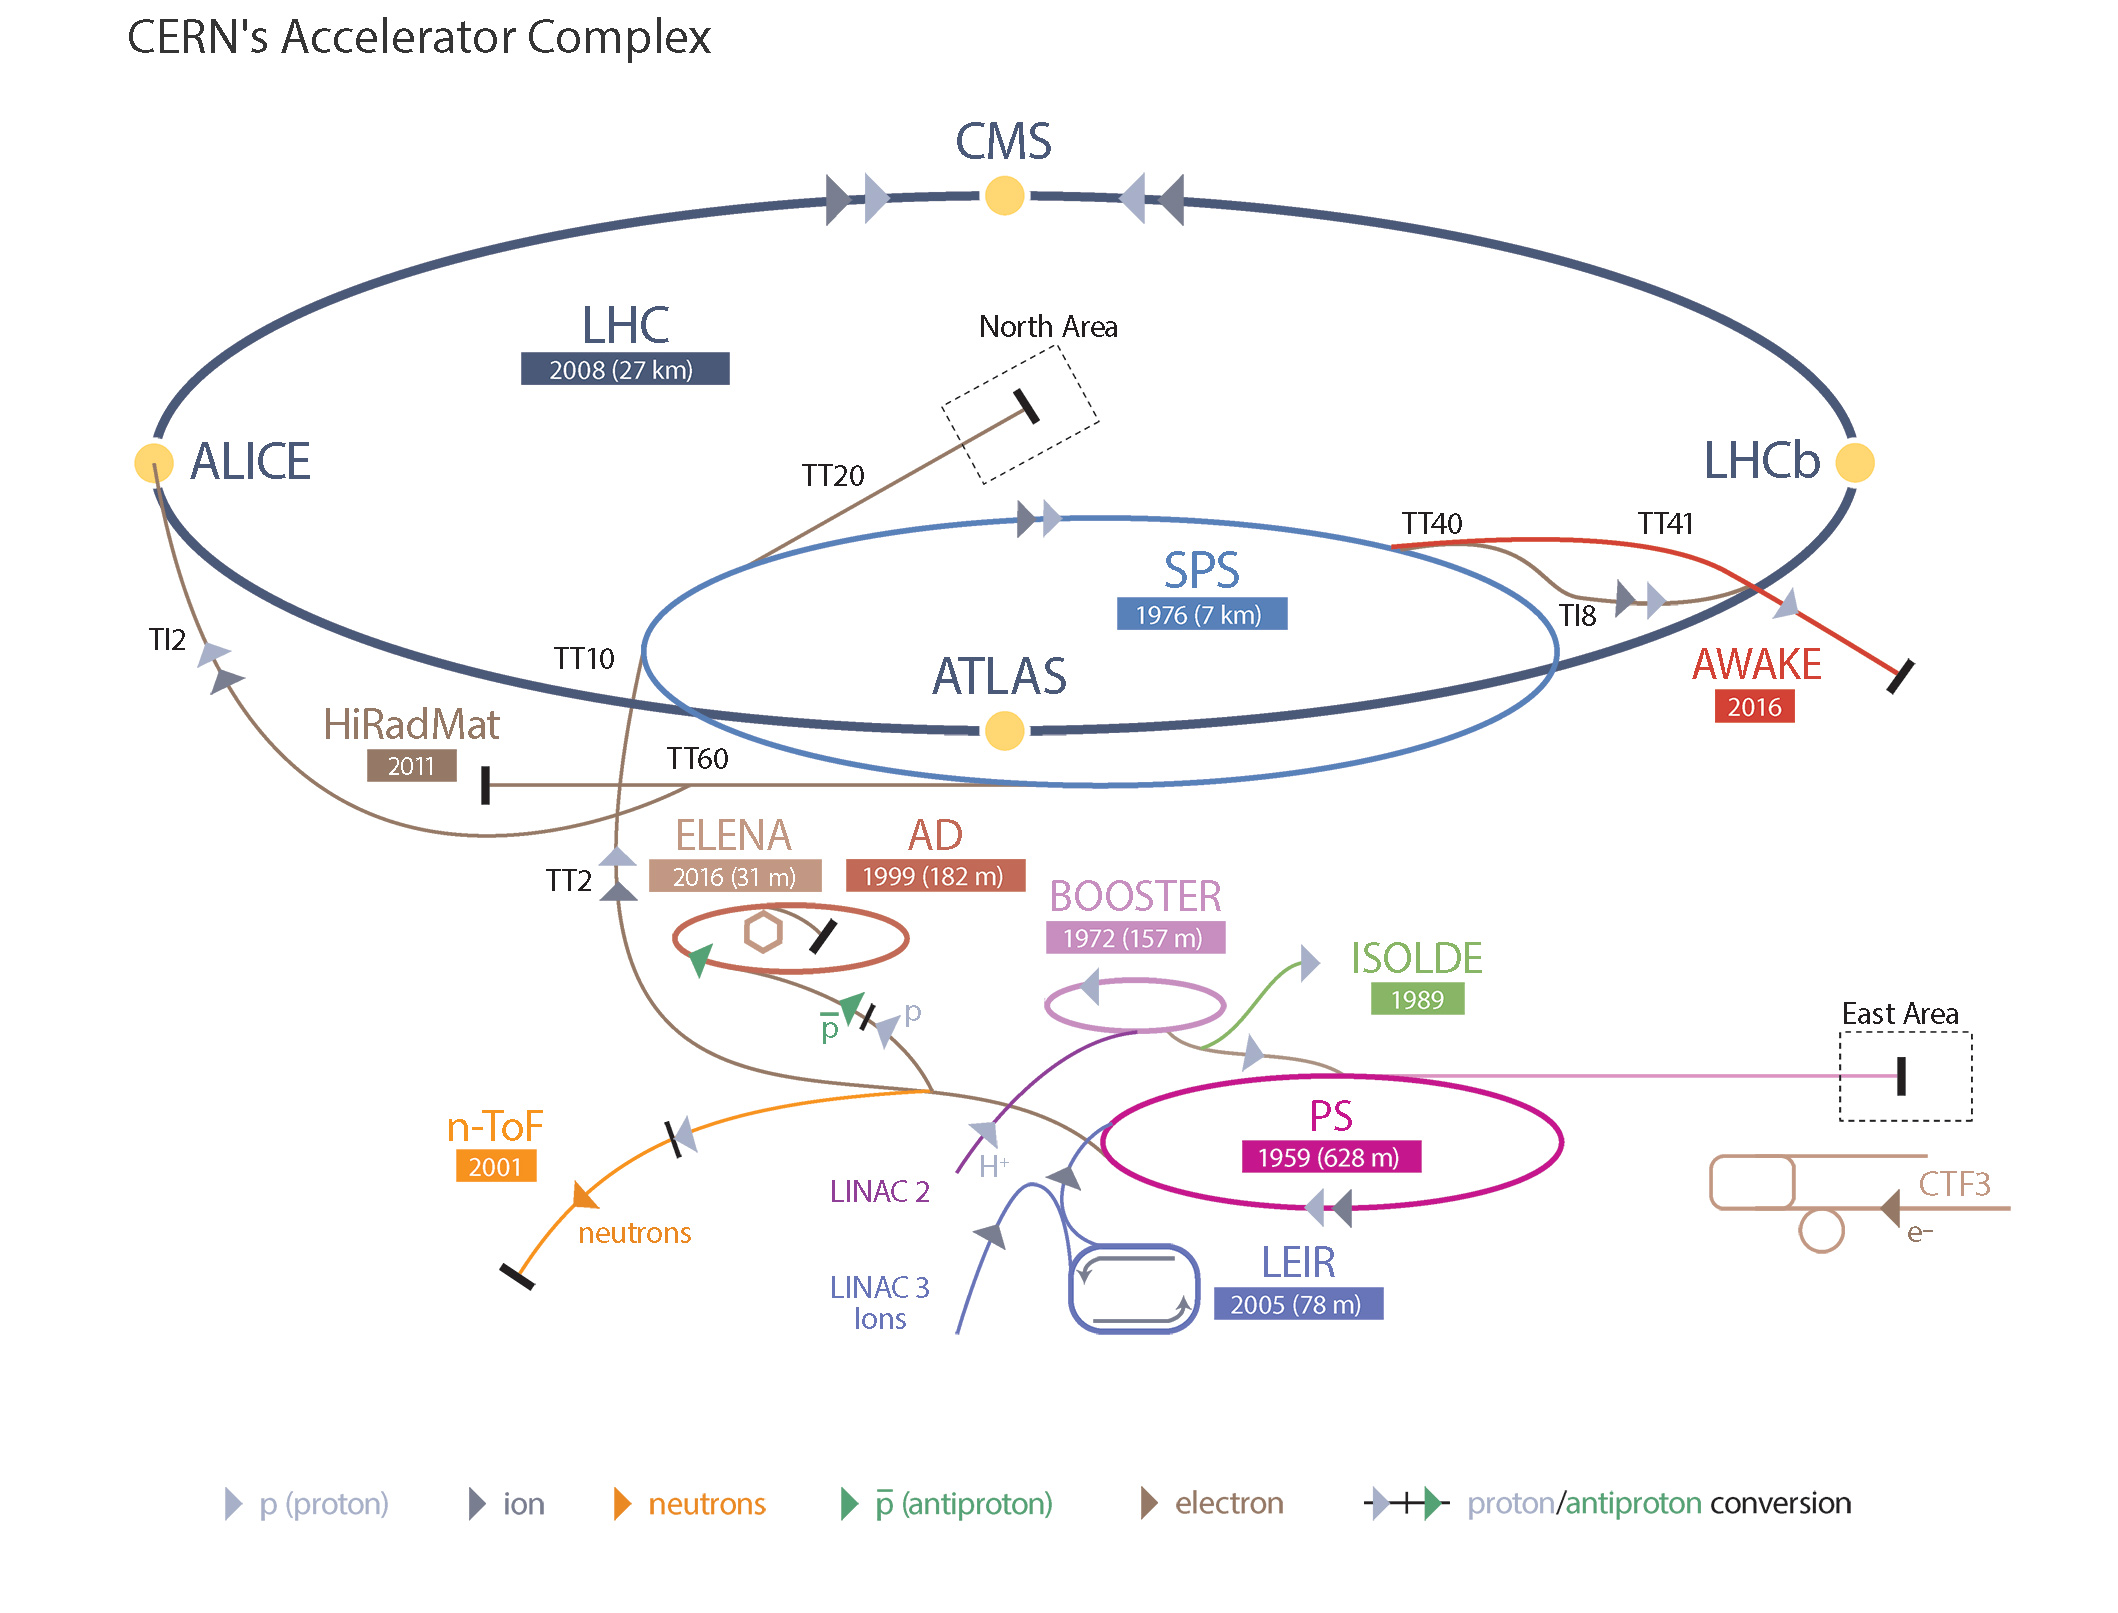
\includegraphics[width=\linewidth]{figures/detector_chapter/LHCRing.png}
  \caption{The infrastructure of the LHC accelerator ring, including the SPS and LINAC2. \cite{LHCRing}}
  \label{fig:LHC}
\end{figure}

The tight bunching of protons by the LHC ring allows the collider to deliver collisions at a high luminosity, a measure of the number of expected collision events per unit of beam area. Luminosity is measured in both instantaneous and integrated form (i.e., 'luminosity per unit time' and total luminosity delivered to date'); as of the end of the second major LHC run, the collider has delivered a total integrated luminosity of $139 fb^{-1}$, equivalent to approximately $1.39*10^{41}$ collisions per square centimeter \cite{ATLAS-CONF-2019-021}. 

The production rate of a given process (that is, number of events of process 'p' produced per unit time) with cross-section $\sigma_{p}$ at a collider delivering instantaneous luminosity $\mathcal{L}$ is given by:

\begin{equation}
\frac{dN_{p}}{dt} = \sigma_{p} \mathcal{L}
\end{equation}

Thus, increasing the luminosity of a collider increases the production rate of rare events as well. At the time of this writing, the LHC is nearing the end of 'Long Shutdown 2' (LS2), a two-year long upgrade period designed to increase detector performance and lay the groundwork for the upcoming high-luminosity LHC (HL-LHC) upgrade, which is slated to begin in approximately 2027 and aims to increase the design luminosity of the LHC by at least a factor of 5 \cite{HLLHC}. Higher luminosity allows for the production of more rare physics events, but also dramatically increases the incidence of unwanted "pileup" events; mitigating this is one of the major efforts of the CERN physics community during the lead-up to the HL-LHC run.

The LHC ring accelerates beams to a center-of-mass collision energy of 13 TeV. The ring consists of two primary beam pipes, one containing a "clockwise" beam and the other containing a "counterclockwise" beam, which overlap at the four primary collision points. These correspond to the four major LHC physics experiments: ATLAS \cite{ATLAS_TDR} and CMS \cite{CMS_TDR}, which are "general purpose" physics detectors, LHCb \cite{LHCb_TDR}, which is specialized to study the physics of hadrons containing bottom (or "beauty") quarks, and ALICE \cite{ALICE_TDR}, which is primarily designed for heavy-ion physics. Due to the highly sensitive nature of their instrumentation, these detectors are buried approximately 100 meters underground to avoid interference from high-energy cosmic rays.

\section{The ATLAS Detector} \label{sec:ATLAS} 

The work contained in this dissertation was performed using the ATLAS (A Large Toroidal LHC ApparatuS) detector. Together with its "sibling detector" CMS (the Compact Muon Solenoid), the ATLAS detector is one of CERN's two "general purpose" detectors, so-called because it is designed to observe a wide variety of high-energy physics phenomena. The ATLAS detector is cylindrical, with a diameter of 25 meters and a length of 44 meters \cite{ATLAS_TDR}. Upon colliding at the interaction point in the center of the detector, the constituent particles of each proton will interact with one another through a host of different physical processes, producing a variety of new particles traveling at high velocities. The ATLAS detector is comprised of several specialized subsystems, each of which is responsible for logging different properties of these decay products. Each of these subsystems is optimized to detect specific properties of a collision event; taken together, they provide a detailed snapshot of the moment of interaction.
	The Inner Detector (ID), a high-resolution detector composed of primarily of silicon, measures the tracks of particles close to the primary vertex. It is encased within a 2T solenoidal magnetic field that bends the tracks of charged particles produced at the collision point, allowing particle momenta to be measured as a function of the curvature of their trajectories. Enclosing the Inner Detector are two nested calorimeter systems: a liquid-argon-and-lead electronic calorimeter (ECAL) that measures the energy of incident photons and electrons, and a primarily scintillator-tile-and-steel hadronic calorimeter (HCAL) that measures the energy of hadronic showers. Finally, a muon spectrometer composed of gas-filled tubes and chambers records the tracks of muons, which do not decay in the calorimeters like most other particles \cite{muonsTDR}.
	The entirety of the muon spectrometer is suffused with magnetic field generated by 24 toroidal magnets, eight of which lie in the barrel, generating a field of 1T and eight of which lie in each endcap, generating a field of 0.5T \cite{DiehlMuons}. These magnets bend the trajectories of muons in a manner similar to the inner solenoidal magnet system, allowing the momenta of particles to be measured based on the track curvature. The ATLAS detector is also equipped with a highly sensitive trigger system, which uses a wide variety of physics signatures in each of these detector subsystems to determine which collision events to store for later analysis \cite{ATLAS_TDR}. A diagram of the ATLAS detector is shown in figure \ref{fig:ATLAS}.

\begin{figure}
  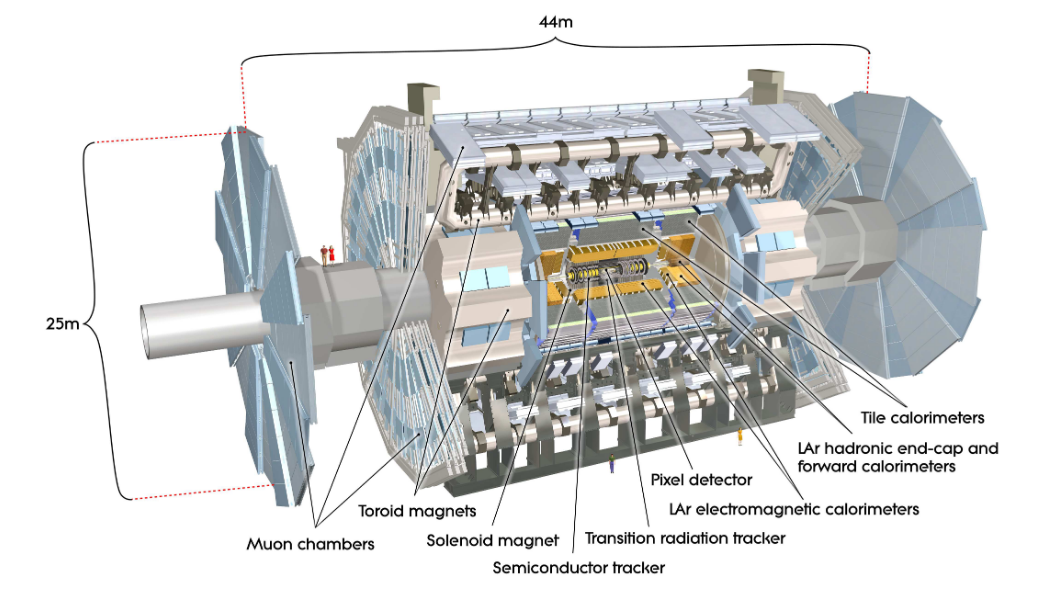
\includegraphics[width=\linewidth]{figures/detector_chapter/ATLAS.png}
  \caption{A diagram of the various subsystems of the ATLAS detector. \cite{ATLAS_Jinst}}
  \label{fig:ATLAS}
\end{figure}

	The ATLAS detector uses a right-handed coordinate system, with the central interaction point at z = 0. The x-axis points from the interaction point to the center of the LHC ring, while the y-axis points upward. However, particle trajectories are more commonly measured not in (x,y,z) coordinate space but utilizing angular variables ($r$ and $\phi$) in the transverse plane and pseudorapidity $ \eta $ in the longitudinal plane, where $ \eta = -ln(tan( \theta /2) ) $ . This is illustrated in figure \ref{fig:coords}.

\begin{figure}
  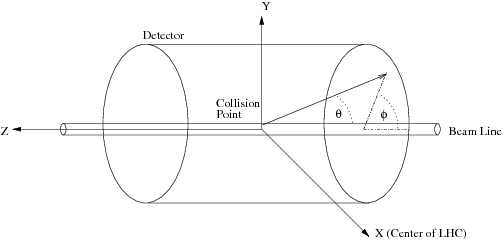
\includegraphics[width=\linewidth]{figures/detector_chapter/coords.png}
  \caption{The coordinate system used to define the ATLAS detector geometry. \cite{coords}}
  \label{fig:coords}
\end{figure}

\subsection{Inner Detector} \label{sec:ID} 

The Inner Detector is composed of five highly granular subdetectors \cite{ID}. The closest to the beam, the silicon-based Insertable B-Layer, was added between the LHC's first and second runs in order to improve precision track-vertex measurement for tasks such as b-hadron tagging and tau lepton identification \cite{IBL_TDR}, methods discussed more in Chapter \ref{chap:methods_chapter}. Proceeding outward from the IBL are the silicon-based Pixel detector and Semiconductor Tracker (SCT), followed by the gas-based Transition Radiation Tracker (TRT) \cite{ATLAS_TDR}. The inner detector is encased within a solenoidal magnetic field which causes charged particle tracks to bend according to their charge, as detailed in Section \ref{sec:solenoid}.

The IBL is composed of 26,880 250×50 $ \mu m^2 $ silicon pixels arranged in an 80 column by 336 row geometry. The pixel modules are supported by 14 support staves, tilted at approximately 14 degrees from the nominal to achieve near-complete cylindrical coverage of the barrel region. The IBL is approximately 33.25 mm from the beam axis, necessitating a replacement of the beryllium beam-pipe with a smaller-radius one for detector reintegration \cite{IBL_TDR}.

Silicon is an optimal material for precision trackers due to its status as a semiconductor. Silicon wafers can be easily "doped" with atoms of other elements, leading them to carry either an excess of electrons (n-type semiconductors) or a deficit of electrons (p-type semiconductors). By putting the two together, an n-p junction is formed, leading to a one-way current gate known as a diode. A voltage is then applied to the diode to halt current flow ("reverse biasing"). When ionizing particles such as those produced in collisions pass through the silicon, they will produce a cascade of charge carriers that will induce a current in the diode, which can then be measured by the precision front-end electronics attached to the silicon wafers \cite{Knoll}.

The pixel detector is similarly composed of silicon pixels, each of which is either 50x400 $ \mu m^2 $ (nominal) or 50x600 $ \mu m^2 $ (near the front-end readout electronics due to spatial constraints). The detector contains 1744 identical pixel sensors, each of which contains 47232 pixels. Three layers of pixels in the barrel region sit at r = 50.5,  88.5 and 122.5 mm from the beam axis, while three layers of pixels in the endcap region sit at r= 495, 580, and 650 mm from the beam axis. The silicon wafers in the pixel detector are "n+ type" strips (n-type semiconductors with extra doping) embedded in an n-type bulk, rather than the traditional n-type and p-type semiconductors due to the fact that excessive radiation from the beam can cause standard n-and-p-type semiconductors to change into one another \cite{Pixel}. 

The SCT is composed of longer silicon microstrip wafers made out of standard n-p type semiconductors. It consists of four layers of 2112 total silicon microstrip modules in the barrel region and 1976 microstrip modules in the endcap regions, with 770 microstrips per sensor module. The strips are 12cm long and 80 $\mu$m wide; the distance of modules from the beam pipe ranges from radii of r= 299 mm to r= 514 mm in the barrel and r=852.8 mm to r= 2720.2 mm in the endcaps. The SCT is designed using less-costly materials than the TRT and IBL, but serves a valuable complementary function \cite{SCT}.

Finally, the TRT consists of polyimide "straws" filled with a gas mixture (70\% Xenon, 27\% Carbon Dioxide, and 3\% Carbon Tetrafluoride), each 4mm in diameter and 144 cm long. In the center of each straw tube is a 31 $\mu$m in diameter grounded gold-plated tungsten wire filament that serves as an anode. Charged particles travelling through the gas medium will ionize it, producing a cascade of ions that will drift to the anode wire. The TRT is uniquely designed to detect low-energy X-ray transition radiation photons, which allows for better identification of electron candidates \cite{TRT}. The barrel region consists of 73 layers of sensor modules ranging from r= 554 mm to r = 1082 mm from the beam pipe, while the encaps straws, arranged in a "wheel" shape, stretch from r= 852.8 mm to r= 2720.2 mm from the beam pipe. 

Additionally, two Minimum Bias Trigger Scintillators, composed of plastic scintillator tiles, sit on the circular endcaps of the ID in order to provide trigger capabilities in the forward region $ |\eta| > 2.5 $. The MBTS endcap scintillator consists of 2 cm thick polystyrene scintillator disks mounted on each endcap at a distance of 3.6m from the collision point. 

Together, these subsystems form the ATLAS detector's Inner Detector. Each subdetector has a different spatial resolution- the IBL has a resolution of  approximately 10 $\mu m$, the pixel detector has a resolution of 12 $\mu m$, the SCT has a resolution of 16 $\mu m$, and the TRT has a resolution of 130 $\mu m$. The combined effect of these subdetectors is thus to record particle tracks produced in collisions with very high granularity within the range $ | \eta | < 2.5$, allowing for sophisticated physics analyses to be performed. 

\begin{figure}
  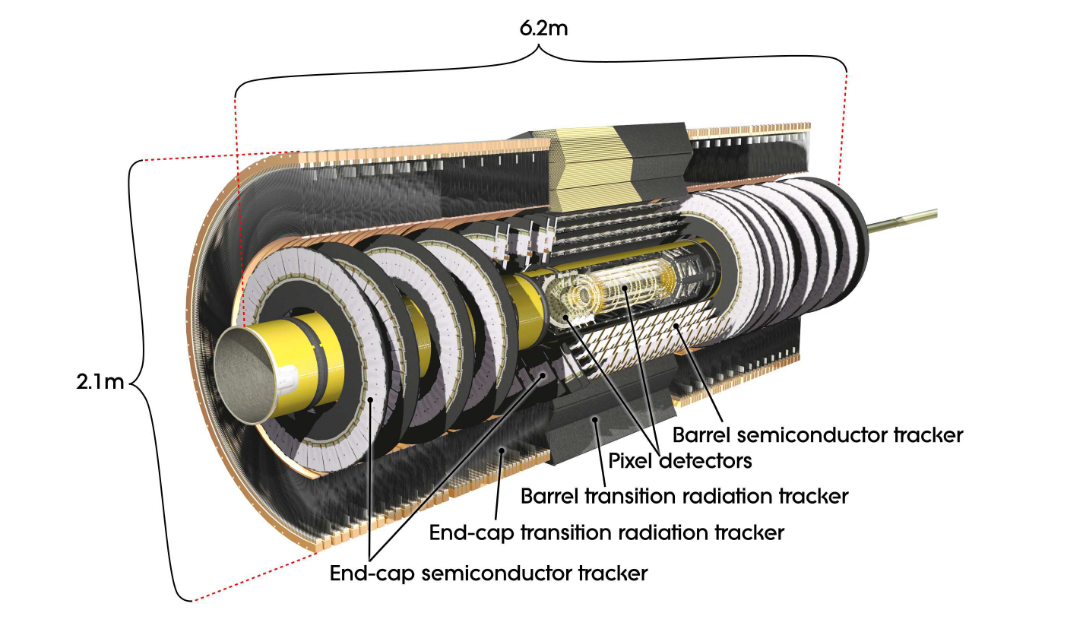
\includegraphics[width=\linewidth]{figures/detector_chapter/ID.png}
  \caption{An illustration of the Inner Detector. \cite{ATLAS_Jinst}}
  \label{fig:ID}
\end{figure}

\subsection{Solenoid Magnet} \label{sec:solenoid}

Track-bending in the Inner Detector is performed by a solenoid magnet providing a field of 2T throughout the ID bulk. The solenoid magnet is constructed of a single layer of high-strength aluminum-stabilized Nb/Ti conductor. The magnetic field it provides is axial (in the $z$ direction), and thus the direction of bending of charged tracks in the ID is in the $\phi$ direction. 

\subsection{Calorimeters} \label{sec:Calos} 

Measurement of particle energies is performed by the ATLAS detector's two calorimeters. Both calorimeters provide a wider $\eta$ coverage than the Inner Detector, allowing for measurement of hadronic jets and electromagnetic showers that fall outside the $|\eta| < 2.5$ precision tracking range. The liquid-argon based calorimeters function differently than the silicon-based tracking Inner Detector: they do not require the incident particles to be charged, and record energies of particles as they shower (decay) in the calorimeter material rather than simply recording their tracks as they pass through. Broadly speaking, there are two types of calorimeters: homogeneous calorimeters, which are composed entirely of active "measuring" material such as liquid argon or polystyrene scintillator tile, and sampling calorimeters, which interleave layers of this active material with slabs of material designed to cause the incident particles to shower \cite{misconceptions}. Both the electronic and hadronic calorimeters are sampling calorimeters; however, they utilize different materials in both the active and non-active layers of the calorimeter. A diagram of the calorimeter system is shown in Figure \ref{fig:Calos}.

\begin{figure}
  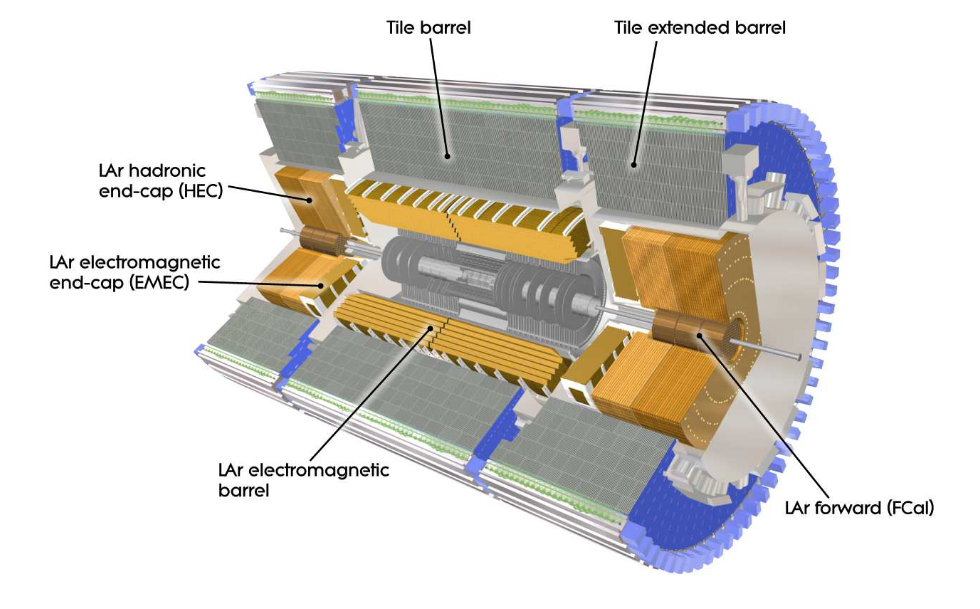
\includegraphics[width=\linewidth]{figures/detector_chapter/Calos.png}
  \caption{An illustration of the ATLAS calorimeter systems. \cite{ATLAS_Jinst}}
  \label{fig:Calos}
\end{figure}


\subsubsection{ECAL} \label{sec:ECAL} 

When electrons and photons enter the non-active layer of a sampling calorimeter, they interact with the electric fields produced by the atoms of the layer material and produce showers of bremsstrahlung photons and electron-positron pairs, which then produce electrical signals in the Liquid Argon active layers that are read out by specialized electrodes. The depth of the electronic calorimeter thus must be chosen carefully in order to capture the entirety of a typical EM shower (measured in "radiation lengths" $X_0$, this varies depending on the absorber material). All ECAL subsystems are made of the same materials: liquid Argon (LAr) sampling layer with lead-plate absorber layers, arranged in a unique "accordion" geometry that gives the ECAL complete coverage in $\phi$ . Due to the high atomic number of lead, the electron clouds of the atoms of the absorber plates are well-populated, thus leading to a high likelihood that photons or electrons will shower within the calorimeter bulk.

The ATLAS electronic calorimeter consists of two primary subsystems: one barrel calorimeter, covering $ |\eta |<1.475$, and two end-cap calorimeters, covering $ 1.375<| \eta |< 3.2 $. The barrel calorimeter is composed of two identical half-barrels, separated by a 4mm horizontal gap at z=0, along the plane of the beam pipe. The lead absorber plates, readout electrodes, and "honeycomb" spacers that form the cavities for the liquid argon layer are all zigzag-shaped and arranged in a circular "starburst" pattern around the barrel \cite{LAr_TDR}, as depicted in Figures \ref{fig:ECALphoto} and \ref{fig:ECALdiagram}. Each half-barrel consists of 1024 accordion absorbers with their associated interleaved spacers and electrodes, weighs 57 tons, and is 3.2 m long, with an inner radius of 2.8 m and an outer radius of 4.0 m. There are three layers of absorbers in the inner precision-measurement region $(0 <| \eta |< 1.35)$ of the barrel and two in the higher-$\eta$ region $(1.35 < | \eta |<1.475)$, each with a different segmentation; the angle, lateral orientation and length of the accordion waves varies with $\eta$.

\begin{figure}
  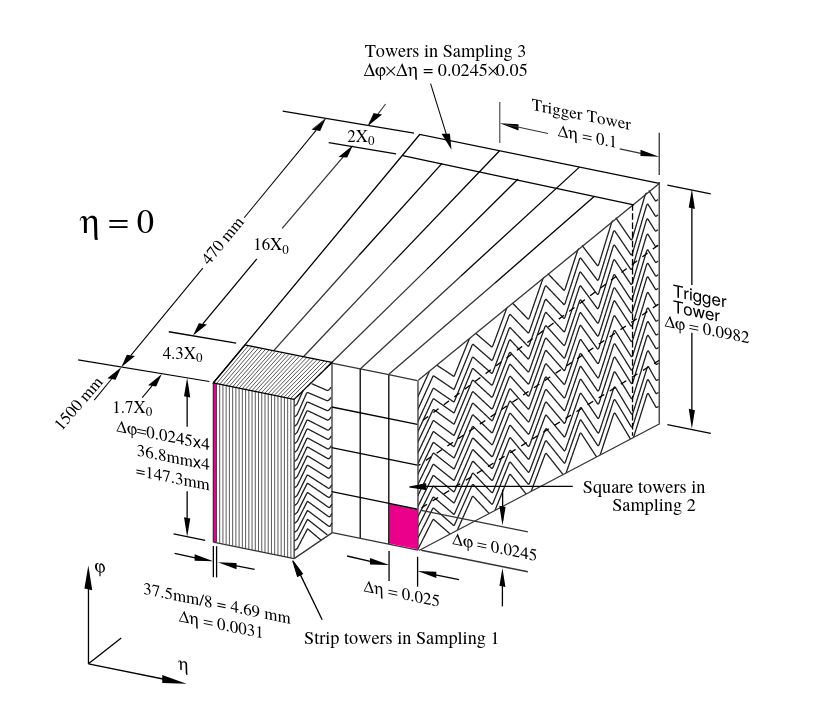
\includegraphics[width=\linewidth]{figures/detector_chapter/ECALdiagram.png}
  \caption{A cutaway diagram of the barrel ECAL depicting the "accordion" absorber geometry \cite{ATLAS_Jinst}}
  \label{fig:ECALdiagram}
\end{figure}

\begin{figure}
  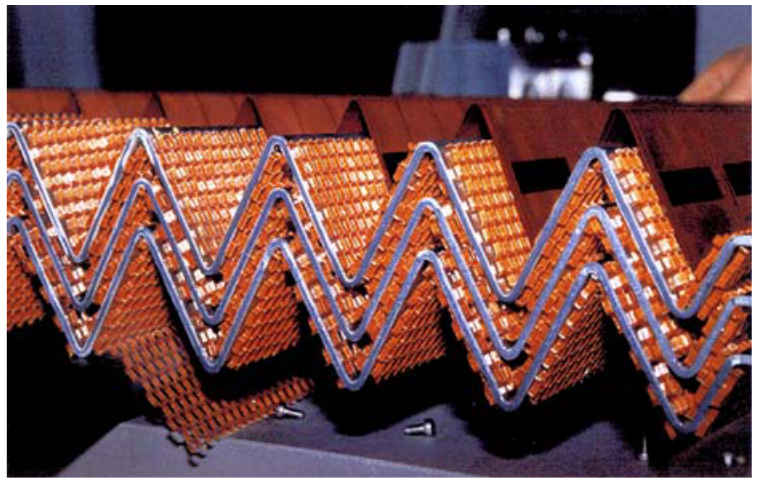
\includegraphics[width=\linewidth]{figures/detector_chapter/ECALphoto.png}
  \caption{A photograph of an ECAL absorber. \cite{KriegerECALphoto}}
  \label{fig:ECALphoto}
\end{figure}

Each end-cap calorimeter is composed of two wheels, one large outer wheel covering $ 1.375<| \eta |<2.5 $, and one smaller inner wheel covering the range $ 2.5<| \eta |<3.2 $. Each endcap is 63 cm thick, weighs 27 tons, and contains 768 accordion absorbers in the outer wheel and 256 absorbers in the inner wheel. Like the barrel, the calorimeter structure in the endcaps consists of three layers of absorber modules in the region nearest the beam pipe in the outer wheel $( 1.5 < |\eta | <2.5 )$ and only two layers both nearest the edges of the outer wheel $(1.375 < |\eta | < 1.5)$ and in the entirety of the inner wheel. In the endcaps, the "zigzag" accordion folds are oriented longways, in the z-direction \cite{Discussion}.

In the barrel, each absorber is at minimum 22 radiation lengths thick (though this varies up to 33 radiation lengths as a function of pseudorapidity $\eta$), thus ensuring that electromagnetic showers are contained within the calorimeter bulk. In the endcaps (except for the outer wheel edge region  $ 1.375< | \eta |< 1.475 $), the calorimeter systems are at minimum 24 radiation lengths thick.

In addition to the accordion sampling layer folds of the ECAL bulk, a presampler detector composed of 64 modules in the barrel and 32 in each endcap provides information about electromagnetic objects before they enter the sampling calorimeter. The presampler modules consist of interleaved electrodes between glass-fiber composite plates, filled with liquid argon in the gaps. In the barrel, the presampler is 11mm thick and covers the entire barrel range; in the endcaps, the presampler is 4mm thick and covers the range $(1.5<| \eta |<1.8)$ \cite{Presampler}.

\subsubsection{HCAL} \label{sec:HCAL} 

Hadronic showers typically have both electromagnetic and non-electromagnetic components, and, as such, are typically much larger than electromagnetic showers  As such, the hadronic calorimeter is required to be much deeper than the electronic calorimeter, in order to longitudinally contain hadronic showers in their entirety. The characteristic length scale for hadronic showers is the nuclear interaction length ($\lambda_{int}$), which can be up to 30 times larger than the radiation length $X_0$. The ratio $\lambda_{int} / X_0 $ is proportional to atomic number; thus, placing at least one layer at the front of a hadronic calorimeter that uses a high-atomic number material such as lead in its absorbers is essential in order to distinguish between purely electromagnetic showers and the electromagnetic components of hadronic showers. For the ATLAS detector, this purpose is served by the ECAL: a significant fraction of the energy of hadronic jets is deposited in the ECAL as electromagnetic activity due to the presence in jets of charged hadrons such as pions. In deeper layers, calorimeter absorbers should be constructed of a dense material such as iron or steel, so that hadrons are able to interact with the nuclei of absorber-layer atoms and produce signals in the active layers \cite{misconceptions}.  

The ATLAS HCAL is composed of three major subsystems: the TileCal, which uses polystyrene scintillator tiles in the active layer and steel in the absorber layer; the LAr endcap calorimeters, which use liquid argon as the active layer and copper as the absorbers; and the LAr forward calorimeters, which use liquid argon as the active layer and contains both copper and tungsten absorber layers.

The TileCal is located immediately behind the electronic calorimeter, and covers the pseudorapidity range $|\eta |< 1.7$. It consists of a central barrel region and two extended barrel regions, one on each side of the detector cylinder, as depicted in Figure \ref{fig:TileCalDiagram}. The central barrel is 5.8 m long and each extended barrel is 2.6m long; all three have an inner radius of 2.28m and an outer radius of 4.25m. This corresponds to a total radial depth of approximately 7.4 $\lambda\_{int}$. Additionally, each subsystem is composed of 64 wedge modules, each spanning $5.625 ^{\circ}$ in $\phi$ . Each wedge consists of a series of trapezoidal scintillator tiles (3mm thick, but varying in width and height depending on position in the wedge) interleaved with steel absorber; two fiber-optic cables connect each scintillator tile to two photomultiplier tubes in order to enable accurate readout. Each tube connects to multiple tiles; these readout channels are structured in order to form a system of calorimeter cells. 

\begin{figure}
  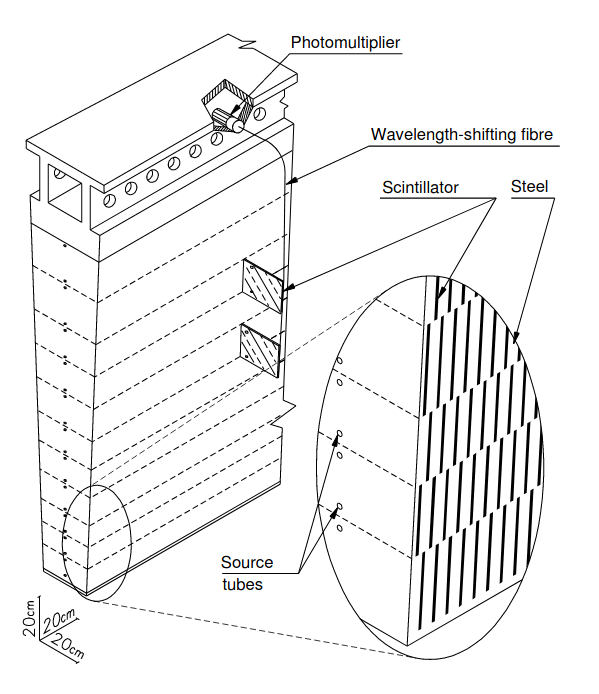
\includegraphics[width=\linewidth]{figures/detector_chapter/TileCal.png}
  \caption{A diagram of the TileCal geometry \cite{ATLAS_Jinst}}
  \label{fig:TileCalDiagram}
\end{figure}

When ionizing particles produced by interactions in the steel absorber reach the scintillator tiles, they produce ultraviolet light. The scintillator tiles are composed of polystyrene doped with 1.5\%  p-terphenyl (PTP) and 0.044\% 1,4-bis(5-phenyloxazol-2-yl) benzene (POPOP), which serve to shift the ultraviolet photons into visible light. These are then read out through the photomultiplier tubes \cite{ATLAS_TDR}.

The Hadronic Endcap Calorimeter (HEC) uses flat copper plates as the absorber layer and liquid argon as the active material, and covers the range  $1.5 < | \eta | < 3.2 $. It consists of two wheels in each endcap, each wheel containing two longitudinal sections. Each wheel is cylindrical with an outer radius of 2030 mm, and consists of 32 identical wedge modules. The front wheels contain 24 copper plates each; the rear wheels contain 16 each.

Finally, the LAr forward calorimeters (FCAL) sit in the very forward region closest to the beamline, $3.1<|\eta |< 4.9$, and are designed to measure the energy of very forward, often low-energy hadronic jets.  The FCAL is unique in that, due to its forward position, it experiences a very large particle flux; it uses very thin active layers in order to mitigate the potential ion buildup this may cause.  The FCAL contains three subdetectors, labelled FCAL1, FCAL2 and FCAL3 proceeding outward from the beamline.

Because it lies outside the eta range of the electromagnetic calorimeter, the FCAL must also contain an electronic calorimeter component in order to capture the electronic components of hadronic showers. FCAL1 is this electronic calorimeter, and uses copper as its active material. It is composed of a matrix of copper plates with circular holes in them, through which are pushed copper electrode rods utilized for readout. The gap between these rods and the plates is then filled with LAr; this setup offers very fine control over the active layer thickness. This can be seen in Figure \ref{fig:FCAL}.

\begin{figure}
  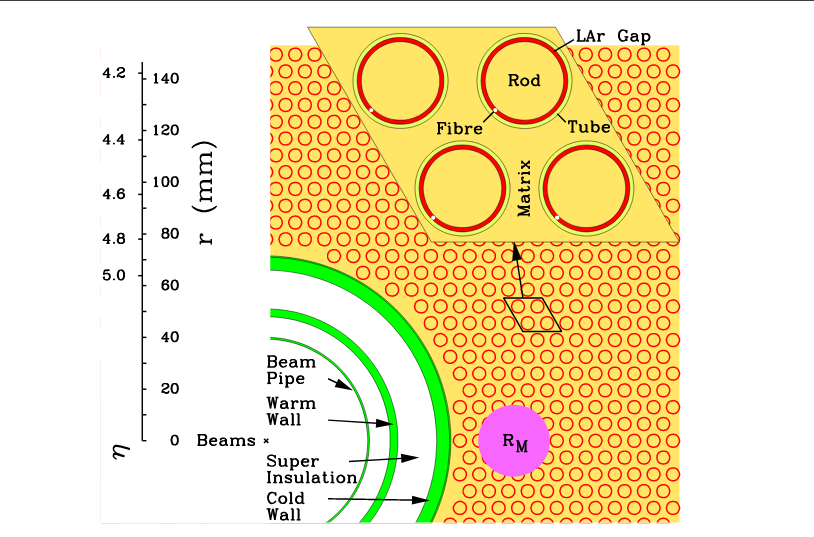
\includegraphics[width=\linewidth]{figures/detector_chapter/FCAL.png}
  \caption{A diagram of the FCAL geometry \cite{ATLAS_Jinst}}
  \label{fig:FCAL}
\end{figure}


FCAL2 and 3, however, are optimized for the much longer characteristic shower scales of hadronic interactions. They are set up identically to FCAL1, but use tungsten readout electrode rods instead of copper \cite{ATLAS_Jinst}.

\subsection{Toroid Magnets} \label{sec:toroids}

A series of three large toroid magnets (one in the barrel and one in each endcap) are designed to curve the tracks of muons in the muon spectrometer, allowing for their momentum to be measured using their curvature. Each toroid consists of eight rectangular air-core coils, wound in the $R - z$ plane. Barrel and endcap toroids are rotated at an angle of $22.5 ^{\circ}$ with respect to each other in order to provide maximal coverage. Because the toroidal magnets are toroids and lie in the $R - z$ plane, they curve tracks in this plane as well; this is distinct from the solenoid, which curves tracks in $\phi$.

Each barrel toroid magnet consists of a "racetrack-style" Aluminum-stabilized Nb/Ti/Cu conductor wound into two double pancakes; together, these supply a field bending-power ranging from 1.5 to 5.5 Tm  in the pseudorapidity range  $0 < |\eta | < 1.4$ \cite{Coldmass}. Endcap toroids are similarly constructed racetrack-style magnets, but are bolted and glued together with eight keystone wedges in order to withstand the Lorentz forces and hold the magnets together. Endcap toroids supply a bending-power of 1 Tm to 7.5 Tm in the range $ 1.6 < |\eta | < 2.7 $ \cite{Toroid} \cite{Magnets}.

\subsection{Muon Spectrometer} \label{sec:Musyst}
 
Unlike electrons and photons, muons are not stopped by the electronic calorimeter. This is due to the fact that a charged particle's energy loss as a function of unit distance due to bremsstrahlung is proportional to its energy and inversely proportional to the square of its mass; because muons are much heavier than electrons, this energy loss drops off substantially at the energies seen at the LHC. While at very high energies, muons again begin to lose most of their energy due to radiation, this occurs at muon energies exceeding a few hundred GeV. Thus, while muons may lose some energy in the electronic calorimeter, and at high energies may be slowed substantially, it is typically not enough to cause them to come to a stop \cite{Stopping}. 

Similarly, because muons do not interact through the strong nuclear interaction, like pions and other hadrons, they are not stopped by the high-Z material of the hadronic calorimeter. Thus, muons in ATLAS are "minimum ionizing particles", that is, particles that lose energy when travelling through material primarily through the process of ionization \cite{PDG}. Therefore, a specialized detector subsystem must be built to measure the energies of muons exiting the detector.

The Muon Spectrometer, is, as its name suggests, not a calorimeter, but a device designed to measure the momentum spectra of outgoing muons (from which their energies can be calculated). It consists of four major types of detector chambers, two designed for muon tracking and two designed for triggering. A cutaway diagram of the full Muon Spectrometer is shown in Figure \ref{fig:MuSyst}.

\begin{figure}
  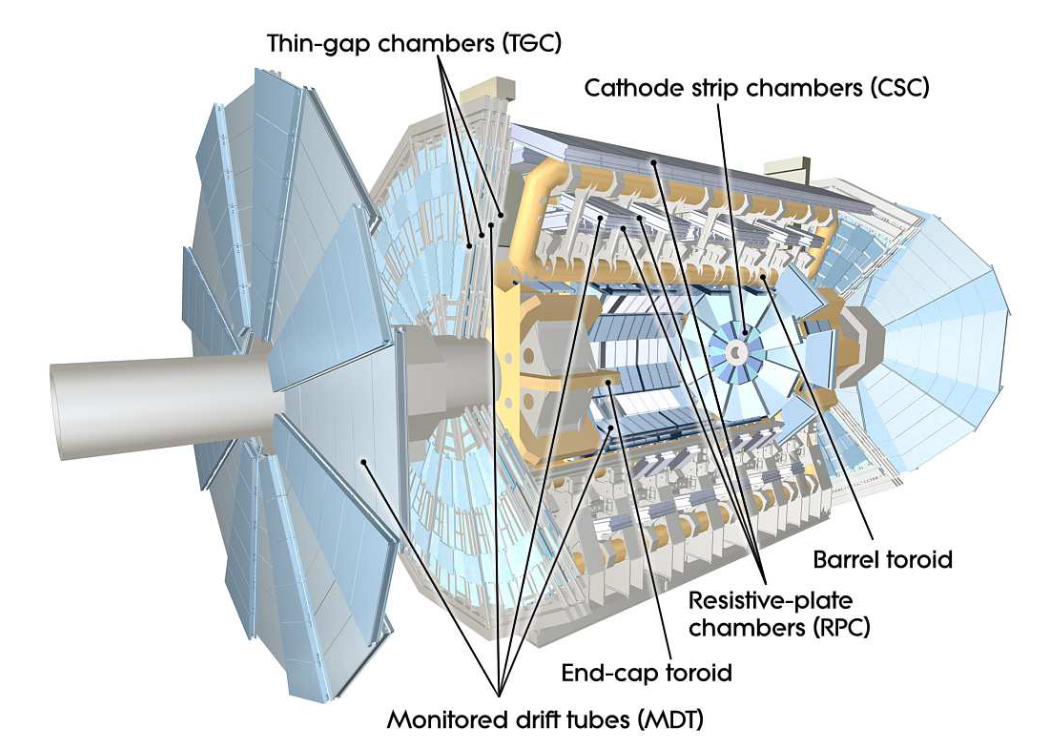
\includegraphics[width=\linewidth]{figures/detector_chapter/MuSyst.png}
  \caption{A diagram of the Muon System \cite{ATLAS_Jinst}}
  \label{fig:MuSyst}
\end{figure}

The primary tracking detectors are the Monitored Drift Tube (MDT) chambers. A single MDT is an aluminum tube 29.970 mm in diameter, threaded through with a 50 $\mu m$ radius tungsten-rhenium wire that is affixed with a stopper at each ends. The tube is pumped through with a mixture of 93\% argon gas and 7\% carbon dioxide, held at a pressure of three bars. Each anode wire is held at a potential of 3080 V, while each tube exterior serves as a cathode, and is grounded. As a muon passes through the tube, it will ionize the gas within; the electrons thus produced will drift to the high-voltage wire and produce electrical signals that can be read out by the specialized boards to which the tubes are attached. Because a muon passing through the tube will leave a trail of ions in its wake, each tube is able to record the minimum radius at which the track passes through the wire, as depicted in Figure \ref{fig:MDT}. However, because this in itself is not enough to reconstruct a track, multiple layers of tubes must be placed together to form a chamber module.

\begin{figure}
  \centering
  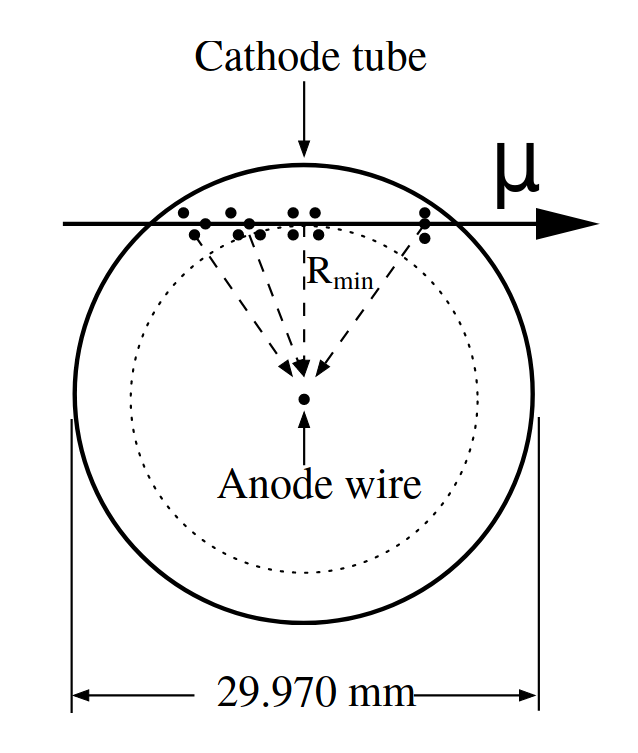
\includegraphics[width=0.5\linewidth]{figures/detector_chapter/MDT.png}
  \caption{A diagram of a Monitored Drift Tube \cite{ATLAS_Jinst}}
  \label{fig:MDT}
\end{figure}

There are 18 varieties of MDT chamber modules, each containing a different number of MDT tubes. Each chamber module consists of one or more "multilayers" of tubes, which consist of either three or four layers of tubes vertically separated by 6.5, 170, or 317 mm, depending on their position in the muon spectrometer. In the barrel, chambers are arranged in three concentric rings around the beam axis, at radii approximately 5m, 7.5m, and 10m from the beamline. In the end-cap region, chambers are arranged in large wheels perpendicular to the beam at approximately 7.4m, 10.8m, 14m, and 21.5m from the interaction point. Each MDT chamber has a spatial resolution of approximately 35 $\mu m$. Overall, MDT chambers cover the region $ |\eta | < 2.7$, though the number of chambers intersected varies as a function of $\eta$. The MDT system geometry is shown in Figure \ref{fig:MDTChamber}. 

\begin{figure}[ht!]
  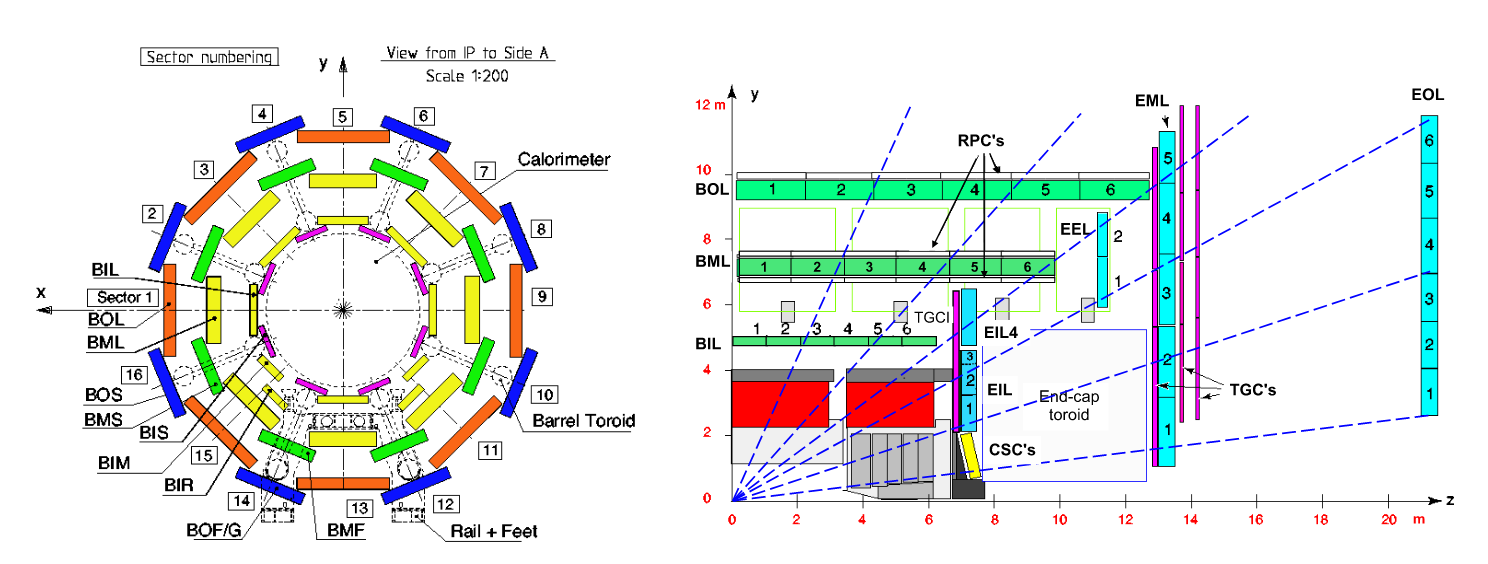
\includegraphics[width=\linewidth]{figures/detector_chapter/MDTChamber.png}
  \caption{A diagram of the MDT chamber geometry from two positions, one looking down the beam pipe and one alongside the detector. \cite{ATLAS_Jinst}}
  \label{fig:MDTChamber}
\end{figure}

Closer to the beam, the event rate is higher due to beam halo effects caused by protons decaying into pions (and in turn, muons) in the beam pipe \cite{Boudreau}. Because the expected rate exceeds the tolerance of the MDT chambers, a different type of muon chamber is situated closer to the beam pipe in order to safely deal with the larger event rate. Cathode Strip Chambers (CSCs), are used in the inner endcap chambers in the range $ 2 < | \eta | < 2.7 $.

Each CSC endcap consist of two circular disks, one containing eight large chambers and one containing eight small chambers. A CSC is a type of multiwire proportional chamber that functions similarly to an MDT: muons passing through the CSC will ionize the $Ar-CO_2$ gas within; electrons will then drift to anode wires and produce a current. Unlike MDTs, however, CSCs are flat, and threaded through with multiple anode wires. Unlike an MDT, a CSC utilizes cathode strips for readout, rather than reading from the anode wire directly: electrons produced during ionization will float to the anode wire; this will produce a charge screening effect that induces a current in the cathode strips. These are then read out; the strength of the current on each strip can be used to determine the path of the muon track.

Each chamber contains eight layers of cathode strips criscrossed with anode wires and filled with a mixture of 80\% argon gas and 20\% $CO_2$. Four of these layers are segmented in the $\eta$ direction and four segmented in the $\phi$ direction, enabling spatial determination of both coordinates of a muon track. Each CSC chamber has a spatial resolution of approximately 40 $\mu m$ in the "bending" $\eta$ plane and 5 mm in the "non-bending" $\phi$ plane. The CSC endcaps are angled slightly toward the interaction point in order to improve resolution; the readout pitch is 5.31mm for the large chambers and 5.66mm for the small ones \cite{CSCs}.

In addition to the precision MDT and CSC chambers, the muon system contains a series of chambers designed explicitly for quickly triggering on muon events. These are the Resistive Plate Chambers (RPCs) and Thin Gap Chambers (TGCs). These provide cursory information about the tracks of muons passing through the detector in order to rapidly determine whether an event should be stored for later analysis.

In the barrel region ($| \eta | < 1.05 $), the trigger chambers are Resistive Plate Chambers (RPCs). RPCs are gas-filled detectors, like MDTs and CSCs, but do not contain a wire. Instead, in each RPC gas-gap module, two resistive plates made of plastic laminate are held 2mm from one another and suffused with a large electric field of 4.9 kV/mm. Incoming muons will then produce ionization avalanches that will induce a current on copper anode strips on the outside of the module through capacitive coupling. RPCs are filled with a gas mixture of 94.7\% 1,1,2,2-Tetrafluoroethane (C2H2F4), 5 \% Isobutane (Iso-C4H10) and 0.3\% Sulfur Hexafluoride (SF6). Each RPC chamber consists of four gas-gap modules, segmented in $\phi$ in a manner similar to the CSCs. RPCs follow the same naming scheme as the MDT chambers, and are arranged in three concentric layers around the detector, one small at radii of 7.820 m, 8.365 m, and 10.229m, and one large at radii of 6.800m, 7.478m, and 9.832m.

In the endcaps $(1.05 <|\eta| < 2.4)$ , the trigger chambers are Thin Gap Chambers (TGCs). TGCs serve two purposes: first, to provide trigger capabilities, and second, to complement the radial measurement of the endcap MDT chambers by providing a precision measurement of the $\phi$ coordinate of incoming muon tracks. TGCs are structured very similarly to CSCs, as they are also multiwire proportional chambers. However, TGCs are designed so the wire-to-cathode distance (1.4mm) is smaller than the wire-to-wire distance (1.8mm). TGCs are filled with 50\% $CO_2$ and 45\% n-pentane (n-C5H12); the choice of this gas in addition to the chamber geometry substantially increases the ratio of charges reaching the wire to ionizations produced by the incident particle. Two layers of copper strips in each chamber are segmented in $\phi$ and used as readout channels.

One set of doublet TGC chambers is placed just inside the inner MDT endcap, covering the range $ 1.05 < |\eta| <1.92 $ (divided radially into two concentric non-overlapping "Endcap" and "Small Wheel" regions); three others (one triplet and two doublets) are placed with the middle MDT endcap to form the "Big Wheel" (covering the range $ 1.92 < |\eta| < 2.4$). On the Big Wheel, TGC chambers are arranged in two circular wheels, each split into 12 segments. The outer wheel (further from the interaction point) contains 48 modules, each subtending 7.5 $^{\circ}$, while the inner wheel (coser to the interaction point) contains 24 modules each subtending 15 $^{\circ}$. Each module contains between 3 and 12 TGCs, depending on its position in the wheel. Similarly, the inner TGC layer is also arranged in a wheel shape, and contains a total of 180 TGCs \cite{ATLAS_Jinst}. The TGC wheels are depicted in Figure \ref{fig:TGCWheel}.

\begin{figure}[ht!]
  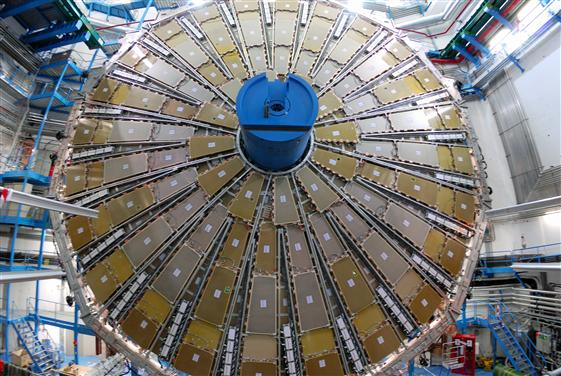
\includegraphics[width=\linewidth]{figures/detector_chapter/TGCWheel.png}
  \caption{A photograph of the TGC wheels. \cite{TGCWheel}}
  \label{fig:TGCWheel}
\end{figure}

\subsection{Trigger} \label{sec:Trigger}
Due to the high rate of collision events delivered by the accelerator, it is impossible to save the data from every single collision produced in the detector. Luckily, only a subset of these are relevant for physics analysis; indeed, the majority of events produced in the detector are "minimum bias" events caused by low-energy interactions between beam protons that are useful only for performance studies \cite{MBTS}. A three-leveled system of triggers is therefore implemented in order to reduce the event rate from 40 MHz to a more manageable 200 Hz. The trigger system is a mix of both hardware and software based subsystems, and is optimized to balance the demands of complexity and speed: more sophisticated algorithms take more time to run, but this cannot get in the way of more data-taking. Each successive trigger is thus more complex than the last, with the lower-level trigger systems applying coarser selections and the higher-level triggers applying finer ones \cite{trigger}.

The first tier of trigger systems, called the L1 trigger, is hardware-based. It utilizes information directly received from the detector subsystems to search for a variety of noteworthy physics objects: high-transverse-momentum muons (transverse momentum here meaning the component of the momentum in the radial coordinate, denoted by $p_T$) are identified using the RPC and TGC chambers discussed in section \ref{sec:Musyst}, while photons, electrons, tau leptons, and hadronic jets are identified using coarse calorimeter information. These triggers form the "L1Muon" and "L1Calo" trigger menus; this information in addition to that of other subsystems such as the MBTS are then sent to the Central Trigger Processor (CTP). The CTP then combines the information from these trigger systems and sends it to the L2 trigger; it also indicates spatial regions of interest using a third trigger called "L1Topo" and calculates quantities of interest such as missing transverse energy (here denoted $E_T^{miss}$, defined as the negative vector sum of the $p_T$ of all objects in the event. $E_T^{miss}$ serves as an indicator of the presence of unobserved neutrinos or other "invisible" decay products in the event). The combined activity of the L1 triggers serve to reduce the event rate to less than 1kHz.

After passing the hardware-based L1 trigger, events then proceed to the software based L2 trigger and Event Filter, which are known together as the High Level Trigger (HLT). HLT triggers utilize a full-granularity event display in order to perform trigger calculations, analyzing the regions of interest marked by the L1 triger. It is at the HLT stage that reconstruction and matching of tracks using Inner Detector information, as well as jet, photon and electron object identification and tagging of objects such as b-jets and tau leptons is performed. All events that pass one or more triggers in the HLT menu are recorded, reducing the event rate to the aforementioed 200 Hz. Triggers may also be 'prescaled' (for which only a set fraction of the events that pass are recorded);this allows analyzers to explore properties of events that normally occur at a rate much higher than can be handled by the trigger system. The triggers utilized in the analyses described in this dissertation are detailed in Chapter \ref{chap:datamc_chapter}.

 

\chapter{Experimental Methods} \label{chap:methods_chapter}
	\section{Experimental Methods} \label{sec:methods} 

It is not possible to induce a particular interaction in a particle collider: every physics process that $can$ occur from the collision of two protons at $13 TeV$ $will$ occur in the ATLAS detector. Thus, the process of studying rare Higgs interactions is not one of determining how to produce them in a laboratory setting, but of determining whether or not they are being produced in our detector at all. Because physics 'signal' processes are fundamentally indistinguishable from unwanted 'background' processes, ATLAS studies are statistical counting experiments which test the compatibility of the observed numbers of events with different detector signatures against the event counts that are predicted to occur under different physics hypotheses. 

Performing these experiments effectively in the data-rich environment of the LHC requires many clever statistical and computational tools, which vary from analysis to analysis. However, in all analyses, it is vitally important both to accurately model what the physics processes of interest may look like in the ATLAS detector and to translate observed detector signals into high-level physics objects. The Monte Carlo simulation method is used for the former, while the latter is performed by the variety of identification and reconstruction techniques detailed in this chapter.

\subsection{Monte Carlo} \label{sec:MC} 

The Monte Carlo simulation method is a way of modelling how a given physics process that may occur at the point of collision may translates into signatures in the ATLAS detector. For a given physics process, say, $gg \rightarrow t \bar{t} H$, we must model both the initial process (i.e., what is the likelihood two gluons will interact to make a $ttH$ event? What properties of the gluons make this more or less likely to occur? How will the top quarks and Higgs boson decay, and what might their decay products look like?), and the detector stage (how will the hadronic jets produced by decaying top quarks and the photons produced by a decaying Higgs look in the ATLAS detector?).

In order to make this problem computationally tractable, each stage is performed separately. In the first stage, the $generator$ stage, physics events for a given process are generated according to their cross-sections $\sigma$ (a measure of how likely they are to occur that is calculated using perturbation theory). A variety of different generator packages are used to produce events for different processes; common generator packages include PYTHIA \ref{Pythia}, HERWIG \ref{Herwig}, and aMCatNLO \ref{aMCNLO}. In many cases, intermediate decays are also performed by the generator software. Meanwhile, detector-level simulation is performed using the GEANT4 (GEometry ANd Tracking 4) package \ref{GEANT4}, which models the signatures of different particles produced in a collision as they pass through detector material.

Simulated events are then reconstructed in the same manner as real events. Because, unlike data events, Monte Carlo events include a "truth record" of what particles they contain, Monte Carlo simulations enable us to perform a number of useful tasks, including training machine learning algorithms to search for specific processes, model the relative contributions of various signal and background processes, and calculate various statistical and systematic uncertainties on our measurements \ref{1005.4568}.

\subsection{Reconstruction and Tagging} \label{sec:Reco} 

Objects produced in the ATLAS detector produce a wide variety of signatures, many of which can be difficult to distinguish from one another. For this reason, dedicated algorithms and criteria are employed to reconstruct and identify the particles used in ATLAS analyses. A sample illustration of the ATLAS detector showing typical shapes of a variety of physics objects is shown in Figure .

\begin{figure}
  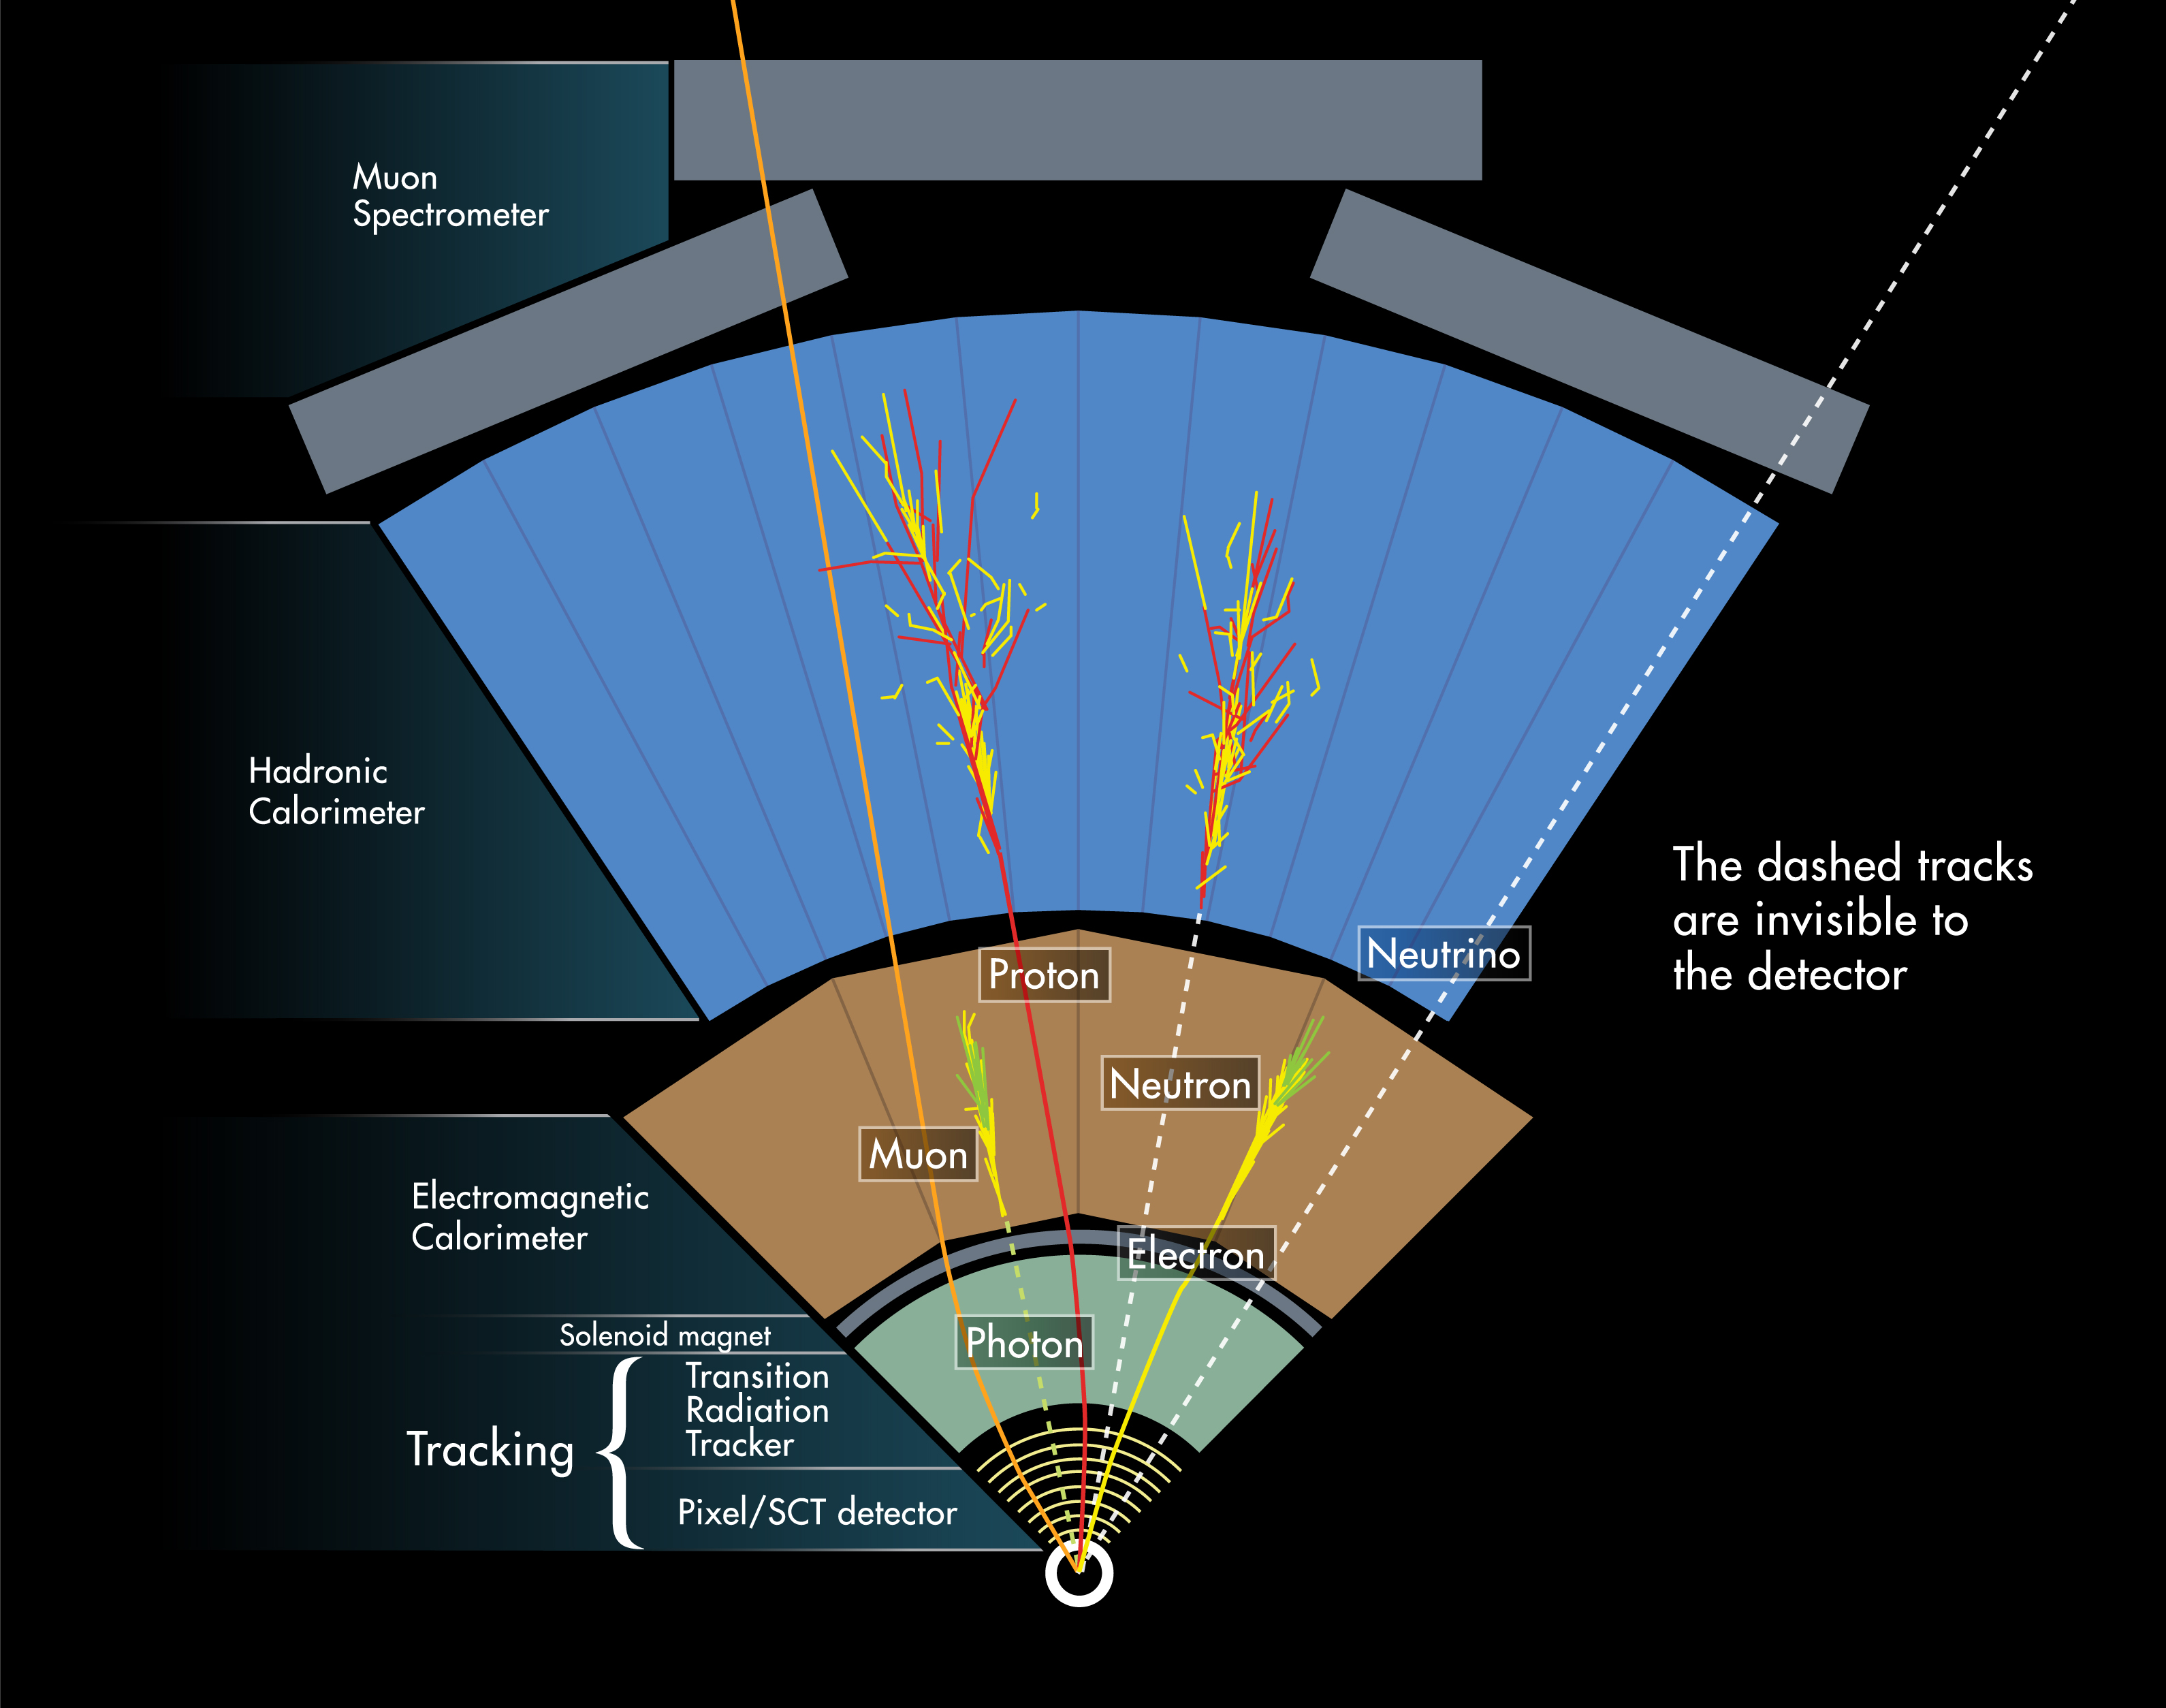
\includegraphics[width=\linewidth]{figures/methods_chapter/Sigs.jpg}
  \caption{Shapes and signatures of a variety of objects in the detector \ref{CERN-EX-1301009}}
  \label{fig:Signatures}
\end{figure}

\subsection{Tracks} \label{sec:Tracks} 

Track reconstruction is essential for identifying and measuring the properties of a wide variety of physics objects, including both muons and hadronic jets.

Initially, the "space points" (spatial coordinates) of potential particle hits are reconstructed using clusters of energy deposits in both the Pixel and SCT detectors. Track candidates are then identified combinatorially using this space-point information (with a minimum of three space-points per track candidate); these track candidates are then passed through an analytic weight-based "ambiguity solver" designed to weed out unphysical track candidates. To aid the ambiguity solver, a neural network is implemented in order to distinguish between isolated and merged clusters of energy deposits. After this, a neural network-based procedure is used to fit the identified tracks. \ref{cite:tracker}.

Fitted tracks from the Pixel detector and SCT can be extended into the TRT if nearby TRT hits are identified. In addition, tracks that are seeded by TRT hits can also be identified and reconstructed using an "outside-in" approach; this helps mitigate the potential loss of real tracks at the ambiguity-solver stage \ref{cite:NEWT}.

After tracks are identified and reconstructed, they are used to identify interaction vertices in the event. Each vertex candidate must contain at least two tracks, each with transverse momentum $p_{T} > 400$ MeV and $|\eta|<2.5$, at least nine hits in the Pixel or SCT detector for tracks with $|\eta|<1.65$ or at least eleven hits for tracks with $|\eta|>1.65$, at least one hit in the first two pixel layers (i.e., the IBL and the inner b-layer), no more than one shared module (i.e. one shared pixel hit or two shared SCT hits), no holes in the Pixel detector, and no more than one hole in the SCT. An iterative combinatorial procedure is then used to fit all compatible tracks to vertex candidates; the primary vertex (PV) representing the initial protom-proton collision is chosen as the vertex with the greatest $\Sigma p_{T}^{2}$ \ref{cite:VertexMeloni}.

However, we note that, for $H \rightarrow \gamma \gamma$ events, a potential lack of charged particles in the final state means that a different primary-vertexing method utilizing ECAL clusters must be considered. This is detailed at length in section \ref{sec:Electrons and Photons}.


\subsection{Clusters} \label{sec:Clusters} 

Photons, electrons and jets are reconstructed using topological clusters of hits ("topo-clusters") in the electromagnetic and hadronic calorimeters. Clusters are reconstructed using a "seed-and-collect" method, where cluster-initiating "seeds" are defined as calorimeter cells with an energy four times greater than the expected noise threshold for that cell  \ref{cite:CERN-EP-2019-145}, \ref{cite:CERN-PH-EP-2015-304}.

After the identification of seed cells, calorimeter cells neighboring the seed cell with recorded energy greater than twice their noise threshold are added to the proto-cluster. If proto-clusters contain more than two local maxima with energy greater than 500 GeV in a single cell, the proto-cluster is split into two in order to account for potential overlap. Initally, seed cells in these split clusters may reside only in the ECAL sampling layers EMB2, EMB3, EME2 and EME3, or the forward calorimeter module FCAL0, after this splitting, clusters are then iteratively split again, with maxima now allowed in the other HCAL and FCAL layers (The first layer of the ECAL is not used to seed topo-clusters in order to reduce the likelihood of producing clusters of noise). In the case of overlap between multiple clusters, cells are assigned to the two cluster candidates with the largest maxima.

\subsubsection{Electrons and Photons} \label{sec:Electrons} 

Electrons and photons are defined using tracks that are matched to topo-clusters in the ECAL. Topo-clusters compatible with EM showers are selected and used to define Regions of Interest; those Regions of Interest are then matched to tracks in the ID. Track candidates are extrapolated into the Regions of Interest using both the measured track momentum and the rescaled momentum measured in the relevant topo-cluster (the latter of which allows for accounting of radiative energy loss in the calorimeter). 

For a track to be considered matched to a topo-cluster, under either momentum-definition-extrapolation, it must fall within $|\Delta \eta| < 0.05$ of its relevant topo-cluster and satisfy $-0.10 < q \times (\phi_{track}-\phi_{cluster}) < 0.05$, where q is the charge of the incident particle. 

Topo-clusters matched to a single charged track are considered to be electron candidates, topo-clusters matched to two oppositely-charged tracks forming a vertex consistent with a photon are considered to be "converted" photon candidates (i.e., clusters resulting from a photon converting into and electron-positron pair in the ID), and topo-clusters matched to no tracks are considered to be "unconverted" photon candidates. In addition, single tracks that have no hits in the innermost layers of the ID are also considered as potential converted photon candidates\ref{cite:CERN-EP-2019-145}. 

Since the start of Run 2, combined topo-clusters called "superclusters" have been implemented in the EM clustering process in order to capture bremsstralung photons and other energy lost in the calorimeter \ref{cite:ATL-PHYS-PUB-2017-022}. For electrons, a supercluster seed must be a cluster with momentum $p_{T} > 1 GeV$ matched to a track with at least four hits, while for photons, a supercluster seed must be a cluster with momentum $p_{T} > 1.5 GeV$. Satellite clusters are then added to the seed to form a supercluster if they fall into a window $\Delta |\eta| \times \Delta\phi = 0.075 \times 0.125$ around the center of the seed cluster. For electrons, an additional satellite cluster search is performed, adding clusters that fall into the window $\Delta |\eta| \times \Delta\phi = 0.075 \times 0.125$ that are matched to the same track as the seed. For converted photons, the $\eta-\phi$ window is not used: all satellite clusters matched to one of the tracks of the converted photon vertex are added to the supercluster.

Following the identification of superclusters and tracks, energy calibration corrections are applied (determined using Monte Carlo simulation for photons and $Z \rightarrow ee$ decays for electrons)\ref{cite:EMcalib}, and the photon and electron candidate objects are passed to cluster-shape-based identification algorithms. For both electrons and photons, three identification working points are defined using cut-based multivariate discriminants based on the shower-shape variables.

For photons, the $loose$ ID threshhold is determined based on the following variables:
\begin{itemize}
  \item Acceptance: $|\eta|<2.37$, excluding the calorimeter crack at $1.37 <= |\eta|<1.52$  
  \item $R_{had}$: the ratio of transverse energy deposited in the HCAL to transverse energy deposited in the ECAL for clusters with $0.8 <= |\eta|<1.37$ 
  \item $R_{had1}$: the ratio of transverse energy deposited in the first layer of the HCAL to transverse energy deposited in the ECAL for clusters with $0.8 <= |\eta|<1.37$ 
  \item $R_{eta}$: the ratio of the energy deposited in the ECAL in a $3 \times 7$ rectangle in the $\eta \times \phi$ plane to the energy deposited in the ECAL in a $7 \times 7$ rectangle in the $\eta \times \phi$ plane, both centered on the calorimeter cell with the most deposited energy. 
   \item Lateral shower width $w_{eta2}$: $\sqrt{\frac{\sigma E_{i} \eta_{i}^{2}}{\sigma E_{i}}-{\frac{\sigma E_{i} \eta_{i}}{\sigma E_{i}}}^2}$ (where E is the energy and $\eta$ is the pseudorapidity of cell 'i', summed over all cells in a $3 \times 5$ rectangle centered around the most energetic calorimeter cell. 
\end{itemize}

The $medium$ photon ID threshold is determined based on both passage of the loose threshold and the variable $E_{ratio} = \frac{E_{1}-E_{2}}{E_{1}+E_{2}}$, where $E_{1}$ and $E_{2}$ are the leading and subleading energies deposited in calorimeter cells, respectively.

The $tight$ photon ID threshold is determined based on passage of the medium ID threshold and the following shape variables in the strip layer of the ECAL
\begin{itemize}
  \item Lateral Shower Width:$w_{s3} = \sqrt{\frac{\sigma E_{i}(i-i_{max})^{2}}{\sigma E_{i}}}$ (where E is the energy of a strip, '$i_{max}$' is the index of the highest-energy strip, and 'i' is the index of each strip with respect to $i_{max}$ calculated in a $3 \times 2 \eta-\phi$  rectangle centered around the strip with the maximum energy deposit
  \item Total Lateral Shower Width:$w_{s tot} = \sqrt{\frac{\sigma E_{i}(i-i_{max})^{2}}{\sigma E_{i}}}$ (where E is the energy of a strip, '$i_{max}$' is the index of the highest-energy strip, and 'i' is the index of each strip with respect to $i_{max}$ calculated in a $20 \times 2 \eta-\phi$  rectangle centered around the strip with the maximum energy deposit
  \item $\Delta E_{s}$: the difference between the second-largest strip energy and the minimum energy in the strips that lie between the largest- and second-largest strip energies
  \item $f_{1}$: The ratio of the energy in the first layer to the energy in the whole EM cluster.
  \item $f_{side}$: the total energy outside the three central strips but within seven strips, divided by the energy of the three central strips 
\end{itemize}

Each working-point threshold varies in bins of $\eta$. For loose and medium working points, converted and unconverted photons are not treated differently, but for tight working points, they are determined separately. \ref{cite:gammaID CERN-EP-2018-216}

For electrons, the identification process proceeds similarly: working-points are defined using shower-shape variables $f_{1}, E_{ratio}, w_{s tot}, R_{eta}, w_{eta2}, f_{3}, R_{had}, and R_{had1},$ as well as $R_{phi}$ (the ratio of the energy deposited in the ECAL in a $3 \times 3$ rectangle in the $\eta \times \phi$ plane to the energy deposited in the ECAL in a $3 \times 7$ rectangle in the $\eta \times \phi$ plane, both centered on the calorimeter cell with the most deposited energy). Electron ID working-points also include the following track variables:
\begin{itemize}
\item $n_{Blayer}$: Number of hits in the B-layer
\item $n_{Pixel}$: Number of hits in the Pixel
\item $n_{Si}$: Number of hits in the silicon detectors (ID and SCT)
\item $d_{0}$: the transverse impact parameter relative to the beamline
\item $|d_{0} / \sigma(d_{0})|$: the impact parameter significance relative to its uncertainty
\item $\Delta(p)/p = (p-p_{last})/p$: the momentum difference between the track perigee and its endpoint, divided by the momentum at perigee
\item $eProbabilityHT$: the electron probability based on TRT radiation
\item $\Delta \eta_{1}$: the difference in pseudorapidity between the cluster position in the first layer and the matched track
\item $q \times (\phi_{track}-\phi_{cluster})$: where $\phi_{track}$ is the momentum-rescaled track extrapolated from the perigee and $\phi_{cluster}$ is the cluster position in the second ECAL layer.
\item $E/p$: ratio of the cluster energy to the track momentum (used for $E_{T} > 150 GeV$ only) 
\end{itemize}

However, the photon identification is a cut-based process, while the electron identification process relies on a likelihood-based discriminant. For the analyses discussed in subsequent chapters, we utilize the $Medium$ electron working point, with an efficiency of approximately 88$\%$ \ref{cite:elID-CERN-EP-2018-273}. Electrons are also required to satisfy $p_{T} > 10 GeV, |\eta| < 2.47$ (excluding the calorimeter crack at ($1.37<|\eta|<1.52$), have track impact parameter significance $|d_{0} / \sigma(d_{0})| < 5$, and satisfy $z_{0} \times sin(\theta) < 0.5 mm$ with respect to the primary vertex \ref{ATL-COM-PHYS-2020-378}.

To aid in modelling, additional photon ID working points are created. These "LoosePrimeN" working points involve photons that pass the 'loose' identification criteria, but fail one or more of N 'tight' identification criteria. The analyses discussed in this dissertation use the LoosePrime4 working point, which is defined as photons passing the Loose identification but failing one or more of the $w_{s3}, f_{side}, \Delta E_{s}$, and $E_{ratio}$ criteria \ref{ANA-EGAM-2018-01}.

To distinguish between photons originating from the hard scatter (i.e., the process of interest in an event) and photons radiated off of other final-state objects, we consider the relative isolation of identified photons. Photons near large amounts of calorimeter activity are likely to be radiative photons ('non-prompt') radiated from final-state particles after the hard-scatter event, while photons that are isolated are more likely to originate from the hard-scatter.

Two types of isolation variables are considered: calorimetric and track-based.

The calorimetric isolation variable employed in the analyses discussed here is $E_{T}^{coneXX} = E_{T,raw}^{isolXX} -E_{T}^{core} - C$, where $E_{T,raw}^{isolXX}$ is the total calorimeter energy in a cone of $\Delta R = XX/100 $ around the electron or photon of interest, $E_{T}^{core}$ is the total calorimeter energy in a $5 \times 7$ rectangle in $\Delta \eta \times \Delta \phi$ around the barycenter of the electron or photon of interest, and C is a correction for pileup and leakage.

The photon track isolation variable employed in the analyses discussed here is $p_{T}^{cone20} = p_{T}^{cone} - p_{T}^{core}$, where $p_{T}^{cone}$ is the total track momentum of all tracks with $p_{T} > 1GeV$ in a cone of $\Delta R = 0.2$ around the photon of interest and $p_{T}^{core}$ is the total track momentum of all tracks with $p_{T} > 1GeV$ matched to the photon candidate. In addition to satifying $p_{T} > 1GeV$, all tracks considered for this metric must also fall within $z= 3mm$ of the diphoton vertex and have $|\eta|<2.5$.

The electron track isolation variable considered is $p_{T}^{varcone20}$, identical to $p_{T}^{cone20}$ except for the fact that, rather than consider a constant-radius cone of $\Delta R = 0.2$, we consider a cone of radius $\Delta R = max(\frac{10}{p_{T}[GeV]}, 0.2)$ \ref{cite:CERN-EP-2019-145}.

Unlike in Run 1, photon isolation cut thresholds are defined as a function of photon energy rather than being fixed. The isolation thresholds used are $FixedCutLoose$ ($E_{T}^{cone20}< 0.065 E_{T}^{\gamma}$ and $p_{T}^{cone20} < 0.05 E_{T}^{\gamma}$) and $FixedCutTight$ ($E_{T}^{cone40}< 0.022 E_{T}^{\gamma} + 2.45 GeV$ and $p_{T}^{cone20} < 0.05 E_{T}^{\gamma}$) for photons and $FCLoose$ ($E_{T}^{cone20}< 0.2 p_{T}$ and $p_{T}^{cone20} < 0.15 p_{T}$) for electrons \ref{cite:ATL-COM-PHYS-2020-378}.

In analyses discussed in this dissertation, the diphoton vertex originating from the Higgs decay is often not the hardest vertex. This is because, in processes such as gluon-gluon fusion ($ggF$), many events contain a low final-state track multiplicity \ref{1408.7084}. The diphoton vertex is therefore identified using a Neural Network, trained on variables including the $photon pointing$ (that is, the vertex position in $z$ most compatible with the shower-shapes observed in the ECAL), the $\Delta \phi$ between the vector sum of the track momenta and the diphoton system (as determined by the ECAL), and the scalar momentum sums $p_{T}$ and $p_{T}^2$ for the tracks in each diphoton vertex candidate \ref{HGAMSTXSINT}. Photon energies and pseudorapidities are corrected to reflect this new vertexing procedure.

The efficiency of the Neural Network diphoton vertex compared to the hardest vertex for a number of targeted physics processes ("STXS bins") for the full Run-2 Couplings analysis is shown in Figure .

\begin{figure}
  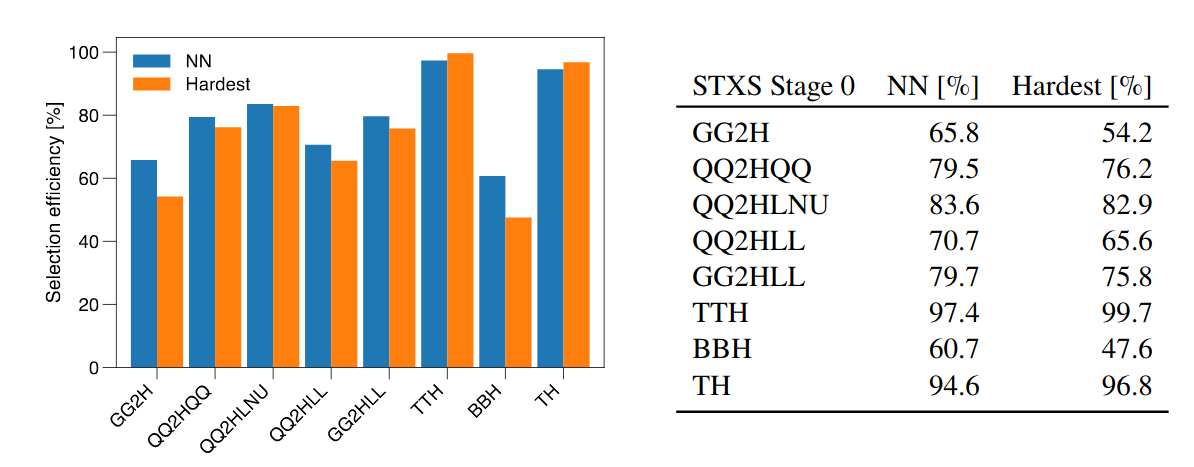
\includegraphics[width=\linewidth]{figures/methods_chapter/Vertexing.png}
  \caption{Shapes and signatures of a variety of objects in the detector \ref{ATL-COM-PHYS-2020-378}}
  \label{fig:Vertexing}
\end{figure}

\subsubsection{Jets} \label{sec:Jets} 

Hadronic jets are identified from topo-clusters using the $anti-k_{t}$ algorithm. Clustering algorithms iteratively follow the following procedure: for each topo-cluster $i$, calculate the distance between both the topo-cluster and every other topo-cluster $j$ and between the topo-cluster and the beam $B$: 

\begin{equation} 
d_{i,j} = min(p_{T,i}^{2k}, p_{T,j}^{2k})\frac{((y_{i}-y_{j})^{2}-(\phi_{i}-\phi_{j})^{2})}{R^2}
d_{i,B} = p_{T,i}^{2k}
\end{equation} 

Where $y_{i}$ is the rapidity of particle $i$, defined as $y=\frac{1}{2} ln(\frac{ E + p_{L}}{ E - p_{L}})$ (where $p_{L}$ is the particle's momentum in the beam direction), $R = 0.4$ (the jet radius), and k is some constant. For the anti-$k_{t}$ algorithm, $k = -1$; other common clustering algorithms use $k=1$ ($k_{t}$) or $k=0$ (Cambridge-Aachen). 

After calculating these metrics, combine the two cluster objects that are the smallest distance apart and re-calculate the distance metrics for the combined object. If a cluster object is closer to the beam than to another object, it is considered a jet and is removed from the list of objects for potential combination.

The algorithm is both infrared safe, meaning that very-low-$p_{T}$ objects do not appreciably impact the jet-finding algorithm results, and collinear safe, meaning that splitting one high-$p_{T}$ object into two collinear ones does not impact the results. Compared to other jet-finding algorithms, the anti-$k_{T}$ algorithm is more robust to the effects of low-energy radiation \ref{antikt}.

For the Run-2 Couplings analysis detailed in section \ref{sec}, the ParticleFlow algorithm detailed in ref \ref{PFlow} is implemented. This helps to provide clearer pictures of the individual constituents of a jet. The ParticleFlow algorithm is an intermediate step in jet reconstruction, which subtracts off energy deposits not associated with the primary vertex and replaces energy deposits that are associated with the primary vertex with the momenta of the relevant tracks. This is done using the modified diphoton vertex discussed previously.

The collection of jets is "cleaned" to remove jets that have signatures consistent with calorimeter noise, and jets that do not satisfy $|y| < 4.4$ and $p_{T} > 25 GeV$ are rejected as well. 

A Jet Vertex Tagger (JVT) multivariate discriminant is also used to reject pileup jets. This utilizes variables such as Jet Vertex Fraction (the $p_{T}$ in a given jet that is track-associated to the primary vertex divided by the $p_{T}$ in a given jet that is track-associated to all vertices) and $R_{pT}$ (the fraction of the $p_{T}$ in a given jet that is track-associated to the primary vertex divided by the total jet $p_{T}$). Different JVT thresholds are used for PFlow Jets and the standard "EMTopo" jets that do not use the ParticleFlow algorithm \ref{cite:JVT}.

\subsubsection{b-jets} \label{sec:b-jets} 

While in general it is very difficult to identify thetype of particle that seeded a hadronic jet, jets originating from hadrons containing bottom quarks are often identifiable with some degree of accuracy. This is due to their long lifetimes compared to other hadrons, meaning that they will travel a short distance in the inner detector (~$450 \mu m$) before hadronizing into jets. 

For EMTopo jets, the Boosted Decision Tree-based Mv2c10 algorithm is used, while for ParticleFlow jets, the Neural Network-based DL1r algorithm is used. The Mv2c10 algorithm is based on a Boosted Decision Tree trained on variables such as impact parameter significance, the presence ad properties of a secondary vertex, and jet kinematic variables such as $p_{T}$ and $\eta$ \ref{cite:CERN-EP-2018-047, CERN-PH-EP-2015-216}; the DL1r algorithm is based on a Deep Neural Network \ref{cite:ATL-PHYS-PUB-2017-013} trained on the same input variables as the Mv2c10 tagger, with additional vertex variables included to allow for charm-quark jet discrimination. The DL1r tagger also features a recurrent neural network trained to take advantage of correlations between track impact parameters in discrimination. The Mv2c10 tagger has an efficiency of approximately 77$\%$, while the DL1r has an efficiency of approximately 70$\%$.  

\subsubsection{Muons} \label{sec:Muons} 

Muons are reconstructed using tracks from either the muon spectrometer and inner detector or the muon spectrometer only.

In the muon spectrometer, segments of hits along the bending plane in the MDT chambers are identified using a Hough transform \ref{Hough}, an image-processing technique from the field of edge-detection that maps observed line segments into a polar-coordinate feature space. The coordinate orthogonal to the bending plane is found using TGC and RPC hits, while segments in the CSC detectors are reconstructed using a separate combinatorial algorithm. Muon tracks are then reconstructed from the segments using a $\chi^{2}$ algorithm- a track must contain at least two segments, except in the barrel-endcap transition region, where one segment is sufficient to build a track. 

Tracks are used to define four types of muons: Combined Muons, for which a track is fitted using both the Inner Detector and Muon Spectrometer, Segment-Tagged, for which a track in the ID is matched to a segment (but not a full track) in the Muon Spectrometer, Calorimeter-Tagged for which a track in the ID is matched to a calorimeter deposit compatible with a muon, and Extrapolated Muons, reconstructed using segments in the Muon Spectrometer that are not associated with any ID tracks but are compatible with the primary vertex. For all muons using the ID, criteria on the number of hits in each ID subsystem are employed to ensure track quality.

Muons must also pass identification criteria to distinguish them from potential fake muons (usually pions or kaons). Three main criteria are used:

\begin{itemize}
\item The charge-to-momentum ratio significance, defined as the absolute value of the difference between the ratio of the charge and momentum of the muons measured in the ID and MS divided by the sum in quadrature of thecorresponding uncertainties
\item $\rho'$, defined as the absolute value of the difference between the transverse momentum measurements in the ID and MS divided by the $p_{T}$ of the combined track
\item the normalized $\chi^{2}$ of the combined track fit
\end{itemize}

The analyses detailed in this thesis use the Medium identification working point, which allows only Combined and Extrapolated muons. Medium Combined Muons require at least 3 hits in at least two MDT layers, except for tracks in the $|\eta| <0.1$ region, where tracks containing at least one MDT layer but no more than one MDT hole layer are allowed. Medium Extrapolated muons require at least three MDT or CSC hits, and are only used in the region $2.5 < |\eta| < 2.7$. Additionally, the q/p significance is required to be less than 7 \ref{CERN-EP-2016-033}. 

Like other objects, we require isolated muons. Muon isolation variables are defined identically to those of electrons for the ttH-CP analysis, while for the Couplings analysis, the ParticleFlow algorithm is used to augment the isolation procedure with a new isolation variable called $neflowiso$, corresponding to the energy deposited in neutral reconstructed ParticleFlow objects rather than raw calorimeter clusters \ref{ATL-COM-PHYS-2019-177}.

For the standard isolation, we use the $FixedCutLoose$ working point, corresponding to $E_{T}^{cone20}<0.30 \times p_{T}^{\mu}$ and $p_{T}^{varcone30}<0.15 \times p_{T}^{\mu}$. For the ParticleFlow isolation, we use $(ptvarcone30+ 0.4\times neflowisol20) <0.16 \times p_{T}$ for muons with $p_{T} < 50GeV$ and $(ptvarcone20+ 0.4\times neflowisol20) < 0.16 \times p_{T}$ for muons with $p_{T} > 50GeV$.

Additionally, muons are required to satisfy $p_{T} > 10 GeV, |\eta| < 2.7$, have track impact parameter significance $|d_{0} / \sigma(d_{0})| < 3$, and satisfy $z_{0} \times sin(\theta) < 0.5 mm$ with respect to the primary vertex \ref{ATL-COM-PHYS-2020-378}. Muon momentum and energy scale and resolution calibrations are determined using $J/\psi \rightarrow \mu \mu$ and $Z \rightarrow \mu \mu$ decays \ref{cite:muCalib}. A charge-dependent sagitta bias calibration is also applied to correct for a slight observed misalignment of the muon system and inner detector.

\subsubsection{Overlap Removal} \label{sec:Overlap}

An overlap removal procedure is employed to avoid double-counting objects. It proceeds in the following order:

\begin{itemize}
\item Remove electrons within $\Delta R=0.4$ of any photon
\item Remove muons within $\Delta R=0.4$ of any photon
\item Remove jets within $\Delta R=0.4$ of any photon
\item Remove jets within $\Delta R=0.2$ of any electron
\item Remove electrons within $\Delta R=0.4$ of any jet
\item Remove muons within $\Delta R=0.4$ of any jet
\end{itemize}

\subsubsection{MET} \label{sec:MET}

The initial momentum of protons approaching the collision point is almost entirely in the beam direction, that is, there is no appreciable momentum component in the transverse direction. Thus, by conservation of momentum, we expect that, when we sum the momenta of all particles produced in the event, we should not see an appreciable momentum excess in the transverse direction. However, often such an excess does occur, indicating the presence of undetected particles that have caused the visible transverse momentum imbalance. Missing Transverse Energy, or MET, is something of a misnomer, as it is missing $momentum$, not energy, but it is one of the most valuable tools for studying rarely-interacting particles such as neutrinos in the ATLAS detector.

The MET is defined as the negative vector sum of the transverse  momenta of all objects associated with the diphoton vertex, including electrons, photons, muons, jets, and any additional low-$p_{T}$ tracks. For the purpose of MET reconstruction in $H \rightarrow \gamma \gamma$ events, $\tau$ leptons are treated as jets; this is allowable because they occur rarely in the parameter spaces studied and decay dominantly to hadrons \ref{cite:CERN-EP-2017-274}.

\subsubsection{taus} \label{sec:taus}
We note that, though many physics analyses use $\tau$ leptons, they are not considered in any of the event signatures discussed in this thesis, so we refrain from discussing their reconstruction at length. However, we note that tau leptons can decay both hadronically and leptonically; as a result of this, their reconstruction depends on the reconstruction of electrons, muons, and jets.
 

\chapter{Data and Monte Carlo Samples} \label{chap:datamc_chapter}
	\section{Data, Monte Carlo, and HGam Pre-selection} \label{sec:DataMC}

\subsection{Data} \label{sec:Data}

In both Run-2 HGam analyses discussed in this dissertation, we use the full LHC Run-2 dataset, consisting of $139.0 \pm 2.4 fb^{-1}$ of proton-proton collisions with a center of mass energy $\sqrt{s} = 13 TeV$ recorded by the ATLAS detector between 2015 and 2018 \ref{Jennet106}. Figure \ref{fig:datalumi} shows the instantaneous luminosity gathered by the detector as a function of time; figure \ref{fig:pileup} shows the number of pileup events per bunch-crossing as a function of time. 

\begin{figure}
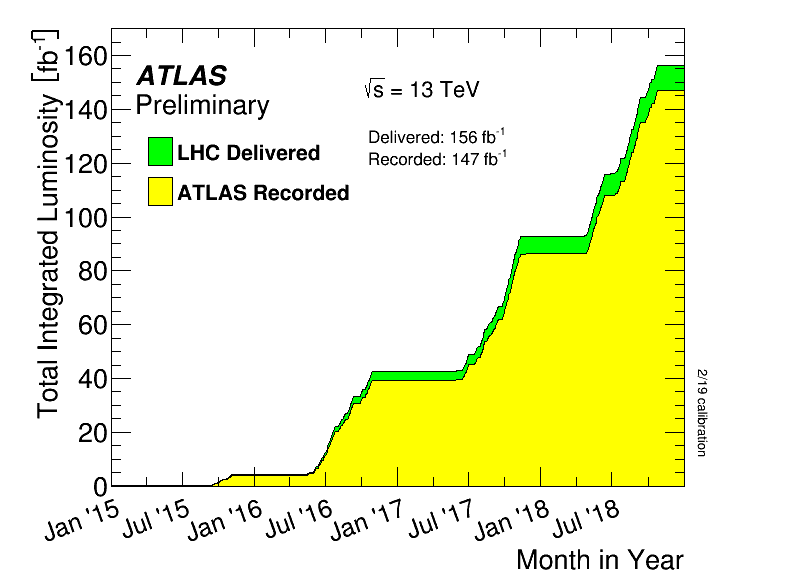
\includegraphics[width=\linewidth]{figures/datamc_chapter/datalumi.png}
\caption{Integrated luminosity for the Run-2 ATLAS data-taking period.}
\end{figure}

\begin{figure}
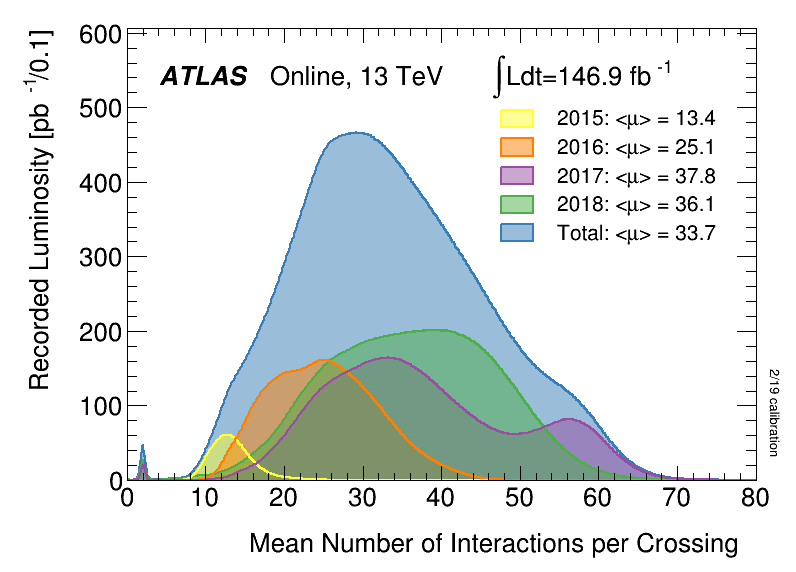
\includegraphics[width=\linewidth]{figures/datamc_chapter/pileup.png}
\caption{Pileup for the Run-2 ATLAS data-taking period.}
\end{figure}

The trigger used to select events is the diphoton trigger HLT\_g35\_loose\_g25\_loose (for 2015-2016 data) and HLT\_g35\_medium\_g25\_medium (for 2017-2018 data). Both triggers require two photon candidates, one with a transverse energy $E_{T}$ of at least 35 GeV and the other with transverse energy of at least 25 GeV. The 2015-2016 trigger requires two photons that pass the "loose" ID requirement, while the 2017-2018 trigger requires two photons that pass the "medium" ID requirement (the cut was tightened due to increased luminosity and pileup). The trigger was calibrated using radiative Z decays, and is observed to be greater than 95\% efficient for each photon as long as it is 5 GeV above the trigger threshold \ref{cite:TriggerPerformance}.

\begin{figure}
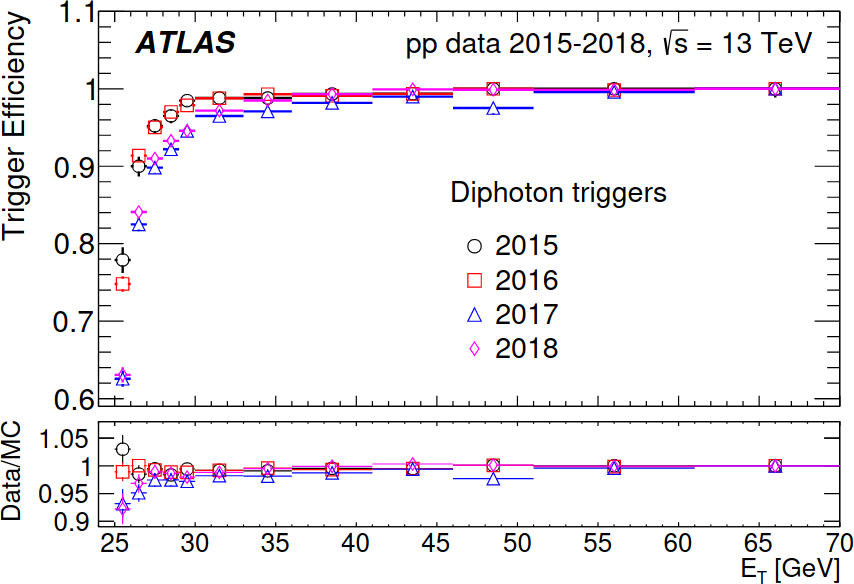
\includegraphics[width=\linewidth]{figures/datamc_chapter/trigger.png}
\caption{Efficiency of the trigger for the different years of the run-2 data taking period as a function of subleading photon $E_{T}$.}
\end{figure}

\subsection{Higgs Preselection and Data CRs} \label{sec:Preselection} 

In both analyses discussed in this dissertation, we use the following preselection to define the $H \rightarrow \gamma \gamma$ signal region. These requirements are applied for both data and Monte Carlo simulation. 

\begin{itemize}
\item $\gamma\gamma Preselection$: The event is required to contain two photons passing the loose isolation and ID requirements.
\item $PV$: At least one primary vertex is required to be identified in the event.
\item $Trigger-Matching$: The leading two photons observed are required to match those identified by the trigger.
\item $Relative p_{T}$: The leading and subleading photons are required to have $p_{T}/m\gamma\gamma$ larger than 0.35 and 0.25, respectively.
\item $TI$: For events in the signal-region, we require both photons to pass the "Tight" Photon ID and Isolation requirements (for events in the 'NTI' data control region, this selection criterion is ignored). 
\item $Invariant Mass$: The invariant mass of the diphoton system must satisfy $105 GeV < m_{\gamma\gamma} < 160 GeV$
\end{itemize}

In order to accurately model the continuum diphoton background, it is often useful to invert the $TI$ requirement- that is, we construct a data sample consisting of those events passing all other preselections, but for which one or more photons does not pass either or both of the "tight" isolation and ID requirements. Data control samples in this not-tight-isolated "$NTI$" region allow us to model the kinematic properties of objects in the event other than the diphoton system, such as top quark jet variables, with some amount of accuracy.

Additionally, it is useful to consider the $TI$ or $NTI$ data sidebands- this consists of the set of events passing either $TI$ or $NTI$ selection with either $105 GeV < m_{\gamma\gamma} < 120 GeV$ or $130 GeV < m_{\gamma\gamma} < 160 GeV$. This allows us to model the shape of the background while safely away from the Higgs signal peak near 125 GeV. This is detailed further in the subsequent analysis-specific chapters.

\subsection{Nominal and Alternative Monte Carlo Samples} \label{sec:NominalMC} 

In order to generate Monte Carlo simulated events, several software programs must work in concert. In a real physics event, different proton constituents (usually gluons or quarks, often called "partons"), interact with one another in a process called a hard scatter to produce new particles. 

To simulate such a collision, the quantum field-theoretic "matrix element" that governs the dynamics of the hard-scatter process must be calculated, the momentum distributions of the individual partons must be modelled using Parton Distribution Functions (or PDFs), and the decay showers of any final-state hadrons produced in the event must be dynamically modelled. Additionally, the dynamics of proton constituents not contributing to the hard scatter, called the "underlying event", must also be simulated. Because showering and underlying event processes are difficult to accurately model, they are "tuned" on the data using a variety of particular parameter sets \ref{cite:tunes}. 

A list of the versions and purposes of the Monte Carlo generator tools is detailed in Table \ref{Table:MCTools}. 

\begin{table}[h]
    \centering
    \begin{tabular}{cccc}
                Purpose & Name & Version & References \\ \hline
				Matrix Element &&& \\                
                & MadGraph5\_aMC@NLO & 8.2.12& \ref{cite:MG5} \ref{cite:aMCNLO} \\
                & Powheg & 7.03 & \ref{cite:Powheg1} \ref{cite:Powheg2} \ref{cite:Powheg3} \\ \hline
                Showering + Matrix Element &&& \\              
                & Pythia8 & 2 & \ref{cite:Pythia1} \ref{cite:Pythia2} \\ 
                & Herwig7 & 2.6.2 & \ref{cite:Herwig1} \ref{cite:Herwig2} \\
                Hadronization &&& \\              
                & EvtGen & 1.1 & \ref{cite:EvGen}  \\
                Matrix Element+Showering+Hadronization &&& \\              
                & Sherpa & 1.2.0 & \ref{cite:Sherpa1} \ref{cite:Sherpa2} \ref{cite:Sherpa3} \ref{cite:Sherpa4} \\
    \end{tabular}
    \caption{Tools used for Monte Carlo generation in the analyses detailed in this dissertation.}
    \label{MCTools}
\end{table}

After generation, Monte Carlo simulations are then passed through the Geant4 software package \ref{Geant4} to simulate the detector response. After this, the events are passed through the same object-reconstruction software used for data events \ref{arXiv: 1005.4568}. All Monte Carlo samples used in this dissertation are generated using the Geant4 full simulation, with the exception of the QCD continuum diphoton samples used for background modelling, which were treated using the GEANT4 fast simulation settings due to the number of events generated. For all MC samples, pile-up interactions were simulated by overlaying each Monte Carlo event with a different number of minimum-bias events simulated using Pythia 8.186 \ref{cite:Pythia} with the ATLAS "A3" tune \ref{cite:A3}.

In all Monte Carlo simulations, the Higgs mass was set to 125 GeV and the decay width was set to 4.07MeV \ref{cite:HiggsWidth}. All samples described include the small contribution from Dalitz decays (that is, decays in which one photon converts into two real final-state leptons), which is accounted for in the normalization of the samples. For all Monte Carlo samples generated using Madgraph5\_aMC@NLO, the renormalization ($\mu_{R}$) and factorization ($\mu_{F}$) scales are defined as the scalar sum of the transverse masses of all final-state particles divided by two (i.e. $H_{T}/2$), and the top and W boson decays are handled by MadSpin \ref{cite:MadSpin} in order to ensure the correct treatment of the spin correlations of the decay products.

For all simulated samples, several corrections are applied to ensure the simulated samples correspond to data, including a beam-spot width correction, photon shower-shape and calorimetric isolation corrections, energy scale and resolution corrections, photon identification and isolation corrections, jet selection efficiency corrections, and electron and muon identification, reconstruction and isolation corrections.

\begin{table}[h!]
  \centering
  \resizebox{\columnwidth}{!}{%
	\begin{tabular}{ |c|c|c|c| }
    	Prod. Mode   &      Generator       & PDF (Matrix Element) & PDF+Tune (Parton Shower)\\ 
		\hline
		    \ggH    &  \NNLOPS + \PYTHIA   & \PDFLHC  &  AZNLOCTEQ6   \\
			\VBF    &      \POWPYTHIA      & \PDFLHC  &  AZNLOCTEQ6   \\
  			$W^{+}H$  &      \POWPYTHIA      & \PDFLHC  &  AZNLOCTEQ6   \\
			$W^{-}H$  &      \POWPYTHIA      & \PDFLHC  &  AZNLOCTEQ6   \\
			$qq\to ZH$ &      \POWPYTHIA      & \PDFLHC  &  AZNLOCTEQ6   \\
			$gg\to ZH$ &      \POWPYTHIA      & \PDFLHC  &  AZNLOCTEQ6   \\
			\bbH    &      \POWPYTHIA      & \PDFLHC  &  A14NNPDF23   \\
			\ttH    &      \POWPYTHIA      & \PDFLHC  &  A14NNPDF23   \\
			\ttH    & \MGMCatNLO + \PYTHIA &  \NNPDF  &  A14NNPDF23   \\
			\tHbj   & \MGMCatNLO + \PYTHIA &  \NNPDF  &  A14NNPDF23   \\
			\tHW    & \MGMCatNLO + \PYTHIA &  \NNPDF  &  A14NNPDF23   \\
			
		\hline
	\end{tabular}
	}
  \caption{Summary of nominal signal samples}
  \label{tab:signal_samples_pyt}
\end{table}

Nominal gluon-gluon fusion events are simulated using the Powheg NNLOPS tool \ref{cite:NNLOPS} using the PDF4LHC15 PDF set \ref{cite:PDF4LHC}, while the nominal $VBF$, $WH$, $ZH$, and $ggZH$ are all generated using the Powheg generator with the PDF4LHC15 PDF set. Showering is performed with Pythia using the AZNLO tune \ref{cite:AZNLO} and the CTEQ6 PDF set \ref{cite:CTEQ6} for these samples. Nominal Standard-Model $ttH$ and $bbH$ samples are generated using the PowhegBOX tool \ref{cite:PowhegBox} using the PDF4LHC15 PDF set; for these samples, showering is performed with Pythia using the A14 tune \ref{cite:A14} and the NNPDF23 PDF set \ref{cite:NNPDF23}. Nominal $tWH$ and $tHjb$ samples are generated using the Madgraph5\_aMC@NLO generator with the NNPDF30 PDF Set \ref{cite:NNPDF30}, and are showered using Pythia with the A14 tune and the NNPDF23 PDF set. $tWH$ samples are generated using the five-flavor PDF scheme, while $tHjb$ samples are generated using the four-flavor PDF scheme. At first order, NLO corrections to the $tWH$ process contain final-state bottom quark jets that thus lead to interference with the more-common $ttH$ process \ref{cite:DemartintWH}; to resolve this, a diagram subtraction method is used \ref{cite:subtraction}.
Additionally, a $ttH$ sample is generated using the Madgraph5\_aMC@NLO generator with the NNPDF30 PDF Set \ref{cite:NNPDF30} for use with the dedicated $ttH CP$ samples, in order to confirm the validity of the effective field theory model used to generate them.

Alternative Standard-Model samples are developed using Herwig for showering rather than Pythia, in order to evaluate the parton-showering uncertainty. The matrix element generators and PDFs are all the same as for the nominal samples, with the exception of the VBF sample, for which generator weights were unable to be included using the Herwig showering tool (and thus the NNPDF30 PDF is quoted for both the generator and the showering tool). $ggH$, $VBF$, $VH$, $tWH$, $tHjb$ and the supplementary Madgraph5\_aMC@NLO $ttH$ sample are all showered using the H7P1 Tune \ref{cite:H7p1}, and the Powheg $ttH$ sample is showered using the \ref{cite:H7UE} tune.

Additionally, a supplementary $ggH$ sample is generated using Madgraph5\_aMC@NLO containing an additional two partons at the matrix element stage. To avoid double-counting events with additional final-state partons, the "FxFx" merging scheme is employed. This sample is showered with Pythia using the NNPDF30 PDF and the A14 tune.
 
\begin{table}[h!]
  \centering
  \resizebox{\columnwidth}{!}{%
    \begin{tabular}{ |c|c|c|c| }
    	Prod. Mode   &      Generator       & PDF (Matrix Element) & PDF+Tune (Parton Shower)\\ 
    	\hline
		\ggH    &  \NNLOPS + \HERWIG   & \PDFLHC  &  \NNPDF+H7p1  \\
		\VBF    &  \POWHEG + \HERWIG   &  \NNPDF  &  \NNPDF+H7p1  \\
		$W^{+}H$  &  \POWHEG + \HERWIG   & \PDFLHC  &  \NNPDF+H7p1  \\
		$W^{-}H$  &  \POWHEG + \HERWIG   & \PDFLHC  &  \NNPDF+H7p1  \\
		$qq\to ZH$ &  \POWHEG + \HERWIG   & \PDFLHC  &  \NNPDF+H7p1  \\
		$gg\to ZH$ &  \POWHEG + \HERWIG   & \PDFLHC  &  \NNPDF+H7p1  \\
		\ttH    &  \POWHEG + \HERWIG   & \PDFLHC  &  \NNPDF+H7UE  \\
		\ttH    & \MGMCatNLO + \HERWIG &  \NNPDF  &  \NNPDF+H7p1   \\
		\tHbj    & \MGMCatNLO + \HERWIG &  \NNPDF  &     \NNPDF+H7p1      \\
		\tHW    & \MGMCatNLO + \HERWIG &  \NNPDF  &     \NNPDF+H7p1      \\
		\ggH    & \MGMCatNLO + \PYTHIA & \NNPDF   &     \NNPDF+A14       \\
    	\hline
    \end{tabular}
  }
  \caption{Summary of alternative signal samples}
  \label{tab:signal_samples_herwig}
\end{table}  

The cross-sections for all Higgs processes are normalized to the state-of-the-art precision measurements discussed in \ref{cite:Yellowreport} using K-factor scaling factors. The accuracy of the cross-sections is N3LO QCD $+$ NLO Electroweak for $ggH$, NNLO $QCD$ $+$ NLO Electroweak for $VBF$ and $VH$, and NLO QCD $+$ NLO Electroweak for $ttH$, while $tHjb$ and $tWH$ are produced at NLO QCD with no electroweak correction. Additionally, samples are normalized to account for the $H \rightarrow \gamma \gamma$ branching ratio of $2.270 \times 10^{-3}$ calculated with HDECAY \ref{HDecay} and PROPHECY4F \ref{Prophecy}.

\begin{table}[h!]
  \centering
  \resizebox{0.25\columnwidth}{!}{%
    \begin{tabular}{ c|l }
      Prod. Mode & {XSxBR [pb]}   \\
      \hline
    	 \ggH       & 0.1101404   \\
    	 \VBF       & 0.00857833  \\
    	 $W^{+}H$   & 0.00190226  \\
    	 $W^{-}H$   & 0.00120605  \\
    	 $qq\to ZH$ & 0.001724519 \\
    	 $gg\to ZH$ & 0.000278529 \\
    	 \ttH       & 0.001149755 \\
    	 \tHbj      & 0.00016857  \\
    	 \tHW       & 3.44359e-05 \\
         \bbH       & 0.00110390  \\
    	\hline
    \end{tabular}
  }
  \caption{Cross sections times branching ratio values used to normalize each production mode. The values correspond to the state-of-the-art predictions and are taken from the CERN Yellow Report \ref{cite:yellowreport}.}
  \label{tab:signal_samples_norm}
\end{table}  

The background for $H \rightarrow \gamma \gamma$ events is generally treated as a smoothly-falling, continuous distribution in diphoton mass $m_{\gamma \gamma}$. It is comprised of non-Higgs events containing real final-state or initial-state radiated photons, as well as hadronic jets that behave like photons. To model this, a functional-form based data-driven method is used; however, Monte Carlo templates are nonetheless used to facilitate and validate the background modelling.

Both QCD continuum $\gamma\gamma$ +jets production and the various $V\gamma\gamma \rightarrow ll\gamma\gamma$ samples are simulated at leading order in QCD using the Sherpa event generator with the CT10 PDF set \ref{cite:CT10}. Showering is performed using the default Sherpa showering tool. 

$t\bar{t}\gamma\gamma$, one of the leading backgrounds in top-enriched regions, is simulated using Madgraph5\_aMC@NLO with the NNPDF30 PDF set. It is showered using Pythia and tuned using the A14 tune.


\begin{table}[h!]
  \centering
  \resizebox{\columnwidth}{!}{%
  \begin{tabular}{|c|c|c|c|c|}
  	 Prod. Mode   &      Generator       & PDF (Matrix Element) & Showering Tool & PDF+Tune (Parton Shower)\\ 
  	\hline
  	$\gamma\gamma+$0,1(NLO),2,3(LO), \myy $\in$ 50-90 \GeV  & \SHERPA & CT10 & \SHERPA & CT10\\
 $\gamma\gamma+$0,1(NLO),2,3(LO), \myy $\in$ 90-175 \GeV & \SHERPA & CT10 & \SHERPA & CT10\\
         $ee\gamma\gamma$; $\myy>\SI{80}{\GeV}$          & \SHERPA & CT10 & \SHERPA & CT10\\
       $\mu\mu\gamma\gamma$; $\myy>\SI{80}{\GeV}$        & \SHERPA & CT10 & \SHERPA & CT10\\
      $\tau\tau\gamma\gamma$; $\myy>\SI{80}{\GeV}$       & \SHERPA & CT10 & \SHERPA & CT10\\
      $\nu\nu\gamma\gamma$; $\myy>\SI{80}{\GeV}$         & \SHERPA & CT10 & \SHERPA & CT10\\
        $e\nu\gamma\gamma$; $\myy>\SI{80}{\GeV}$         & \SHERPA & CT10 & \SHERPA & CT10\\
       $\mu\nu\gamma\gamma$; $\myy>\SI{80}{\GeV}$        & \SHERPA & CT10 & \SHERPA & CT10\\
       $\tau\nu\gamma\gamma$; $\myy>\SI{80}{\GeV}$       & \SHERPA & CT10 & \SHERPA & CT10\\
            $t\bar{t}\gamma\gamma$ (noallhad)            & \MGMCatNLO & \NNPDF & \PYTHIA & \NNPDF+A14       \\
             $t\bar{t}\gamma\gamma$ (allhad)             & \MGMCatNLO & \NNPDF & \PYTHIA & \NNPDF+A14       \\ 
  	\hline
  \end{tabular}
  }
\caption{Summary of nominal background samples}
\label{tab:bckg_samples}
\end{table}  

\subsection{ttHCP Monte Carlo Samples} \label{sec:ttHCPMC} 

In the $ttH CP$ analysis, an Effective Field Theory (EFT) setting a cutoff scale of 1 TeV, below which no new BSM particles coupling to the Higgs exist, is used to generate Monte Carlo samples. The EFT used is the Higgs Characterization (HC) model \ref{cite: HC}, implemented in the MadGraph5\_aMC@NLO generator with the NNPDF30 PDF set. In all BSM samples generated, we use Pythia for showering with the NNPDF23 PDF set and the A14 PDF set.

As previously mentioned, the top-Higgs interaction term of the Lagrangian in the presence of CP-violation can be parameterized as

\begin{equation}
\mathcal{L} = \kappa_{t} g_{t} \bar{t} (cos(\alpha)+ sin(\alpha) i \gamma^{5} )th
\end{equation}

where $g_{t} = \frac{-m_{t}}{v} = \frac{-173.26 GeV}{246 GeV} = -0.703$ , $\kappa_{t}$ is the dimensionless coupling-strength term ($\kappa_{t}= 1$ in the Standard Model), and $\alpha$ is an angle that parameterizes the CP-mixing strength ($\alpha = 0$ in the Standard Model, $\alpha = \frac{\pi}{2}$ in the fully CP-odd case). The interpretation of the $H \rightarrow \gamma \gamma$ and $ggH$ dependence on $\alpha$ is handled in several different ways, as discussed in \ref{sec:ttHCPresults}.

As in the nominal case, $t\bar{t}H$ and $tWH$ samples are generated using the five-flavor scheme, while the four-flavor scheme is used for the $tHjb$ process. The Standard Model cross-sections and branching ratios for all process are normalized to those given in the CERN Higgs Yellow Report 4 \ref{cite:yellowreport}, in which fixed scales and the five-flavor scheme are used. Those cross-sections are calculated at NLO QCD accuracy (without electroweak correction) for the $tHjb$ and $tWH$ processes, while $t\bar{t}H$ is calculated at both NLO QCD and NLO Electroweak accuracies. $ggH+ 2 jets$ samples are also generated using the MadGraph5\_aMC@NLO generator as the $ggH$ cross-section varies with $\alpha$ and $\kappa_{t}$. To ensure that the W-boson Higgs Coupling is kept constant, $tWH$ samples are generated by treating cos$\alpha \times \kappa_{SM}$=1.


K-factors are then computed to scale the Higgs Characterization Monte Carlo cross-sections to the Yellow Report cross-sections. The obtained K-factors are shown to be similar for different CP mixing angles; thus, the K-factors derived for the SM case can be safely used for the various samples with different $\alpha$ values. 

\begin{table}[h!]
\centering
\begin{tabular}{|c|c|||c|c|}
\hline
$\kappa_{t}$ & $\alpha$\ & cos$\alpha$ & $\kappa_{SM}$\\
\hline
1 & 0(SM, CP-even) & 1 & 1 \\
1 & 15 & 0.965926 & 1.035276 \\
1 & 30 & 0.866025 & 1.154701 \\
1 & 45 (CP max mixing) & 0.707107 & 1.414214 \\
1 & 60 & 0.5 & 2 \\
1 & 75 & 0.258819 & 3.863703 \\
1 & 90 (CP-odd)  & 0.000001 & 10$^{6}$ \\
  \hline \hline
 -1 & 0 & 1 & 1 \\
 0.5 & 0 & 1 & 1 \\
 2 & 0 & 1 & 1 \\
 2 & 45 & 0.707107 & 1.414214 \\
\hline
\end{tabular}
\caption{Parameters used in the HC model in order to allow for CP-couplings only in the top quark sector while fixing the HWW coupling to its SM value by imposing cos$\alpha~\kappa_{SM}$=1. In the first set of samples, $\kappa_{t}$ is fixed to 1 and $\alpha$ is varied. In the second set, $\kappa_{t}$ is set to values different from 1. For $\alpha=90$; due to numerical precision, $\cos\alpha$ strictly equal to 0 can't be generated and thus a value approaching it ($10^{-6}$) and a defined value for kSM ($10^{6}$) are used.}
\label{tab:MCsamples_Parameters}
\end{table}

\begin{table}
  \centering
  \begin{tabular}{|c|c||c|c|c|c|}
    \hline
    \multicolumn{6}{|c|}{Normalized Cross-section(fb)} \\
    \hline \hline
    $\kappa_t$ & $\alpha$ & ttH & tHjb & tWH & ggH\\
    \hline
    1 & 0(SM, CP-even)  & 1.150 & 0.169 & 0.034 & 33.1 \\
    1 & 15              & 1.113 & 0.177 & 0.038 & -- \\
    1 & 30              & 0.995 & 0.207 & 0.048 & -- \\
    1 & 45 (CP max mixing)      & 0.827 & 0.266 & 0.064 & 53.7 \\
    1 & 60              & 0.666 & 0.382 & 0.087 & -- \\
    1 & 75              & 0.545 & 0.548 & 0.116 & -- \\
    1 & 90 (CP-odd)     & 0.500 & 0.753 & 0.150 & 74.4 \\
    \hline \hline
    -1 & 0    & -- & 1.980 & 0.307 & -- \\
    0.5 & 0   & -- & 0.264 & 0.030 & -- \\
    2 & 0     & -- & 0.666 & 0.190 & -- \\
    2 & 45    & -- & 0.570 & 0.226 & -- \\
    \hline
  \end{tabular}
  \caption{NLO cross-sections for the $t\bar{t}H$, $tHjb$, $tWH$, and $ggH$ processes for different CP-scenarios normalized with the K-factor and BR$(H\rightarrow\gamma\gamma)$. The top part refers to MC samples in which $\kappa_{t}$ value is fixed to 1 and $\alpha$ is varied, while the bottom part to samples with $\kappa_{t}$ value different from 1.}
  \label{tab:MCsamples_XS_norm}
\end{table}
 

\chapter{Signal Parameterization, Background Parametrization, and Statistical Methods} \label{chap:sigbkgparam}
	In the analyses discussed in this dissertation, smooth functional forms are used to model both the signal and background. This allows an unbinned likelihood fit to be performed, the preferable statistical analysis method in the lower-statistics $ttH$ regime (an alternative to the binned likelihood fit, also common in ATLAS analyses, which offers more statistics per bin, but a general loss of precision). 

Additionally, parameterizing signal and background in this way allows for the relatively straightforward calculation of several key systematics, including "spurious signal" background mismodelling, photon energy scale, and photon energy resolution.

\section{Signal Modelling} \label{sec:example_section} 

In collider physics analyses, one of the most common forms of signal is a "resonance", a bump in a smooth energy spectrum indicating the presence of a particle with mass given by the center of the resonance bump and lifetime given by the width $\Gamma$ of the resonance bump \cite{Peskin}. The "true underlying form" of resonances generally follow the Breit-Wigner distribution described in \ref{SlowNeutrons}; however, due to detector and beam effects, this form does not accurately describe observed data.

Instead, for both analyses discussed in this dissertation, a "Double-Sided Crystal Ball" (DSCB) function \cite{CB}\cite{DSCB} is used. The function has six parameters, two that describe the shape of its Gaussian core $\mu_{CB}$, and $\sigma_{CB}$, and two that describe the shape of each of its exponential tails: $\alpha_{low}$ and $n_{low}$; $\alpha_{high}$ and $n_{high}$. The function is defined as:

\[f_{DSCB}(m_{\gamma \gamma}) = \begin{cases} 
      e^{\frac{-{\alpha_{low}^{2}}}{2}} (\frac{R_{low}-\alpha_{low}-t}{R_{low}})^{n_{low}} & if t < -\alpha_{low} \\
      e^{\frac{-t^{2}}{2}} & if -\alpha_{low} \leq t \leq \alpha_{high} \\
      e^{\frac{-{\alpha_{high}^{2}}}{2}} (\frac{R_{high}-\alpha_{high}+t}{R_{high}})^{n_{high}} & if t > \alpha_{high} \\
   \end{cases}
\]

where $t = \frac{(m_{\gamma \gamma} - \mu_{CB})}{\sigma_{CB}}$ and $R = frac{n}{\alpha}$. 

To parameterize the signal in each analysis category for both analyses discussed in this dissertation, all Monte Carlo for the various Higgs production modes ($VBF$, $VH$, $ggF$, $ttH$, $tWH$, $tHjb$ and $bbH$) generated using a Higgs mass of 125 GeV are combined. The resulting distribution is then fit with a DSCB function, and a rigid transformation of 0.09 GeV is performed such that the mean of the fitted DSCB corresponds to the experimentally measured Higgs mass of $125.09 GeV \pm 0.21 GeV(stat) \pm 0.1 GeV(syst)$ \cite{Higgsmass}.

Because the Double-Sided Crystal Ball function depends strongly on the photon resolution and energy scale, these systematics can be straightforwardly parameterized in the final fit as variations on $\mu_{CB}$ and $\sigma_{CB}$ \cite{gammaID}. This is one of the primary motivations for using this functional form, rather than a Gaussian or other distribution. Examples of DSCB shapes in five categories targeting two STXS truth bins of the Couplings Analysis are shown in Figure \ref{fig:DSCB}.

\begin{figure}[h]
\centering
\subfloat[$gg \rightarrow H$ ( 1-jet, $120 GeV \le p_{T}^{H} < 200 GeV$)] { 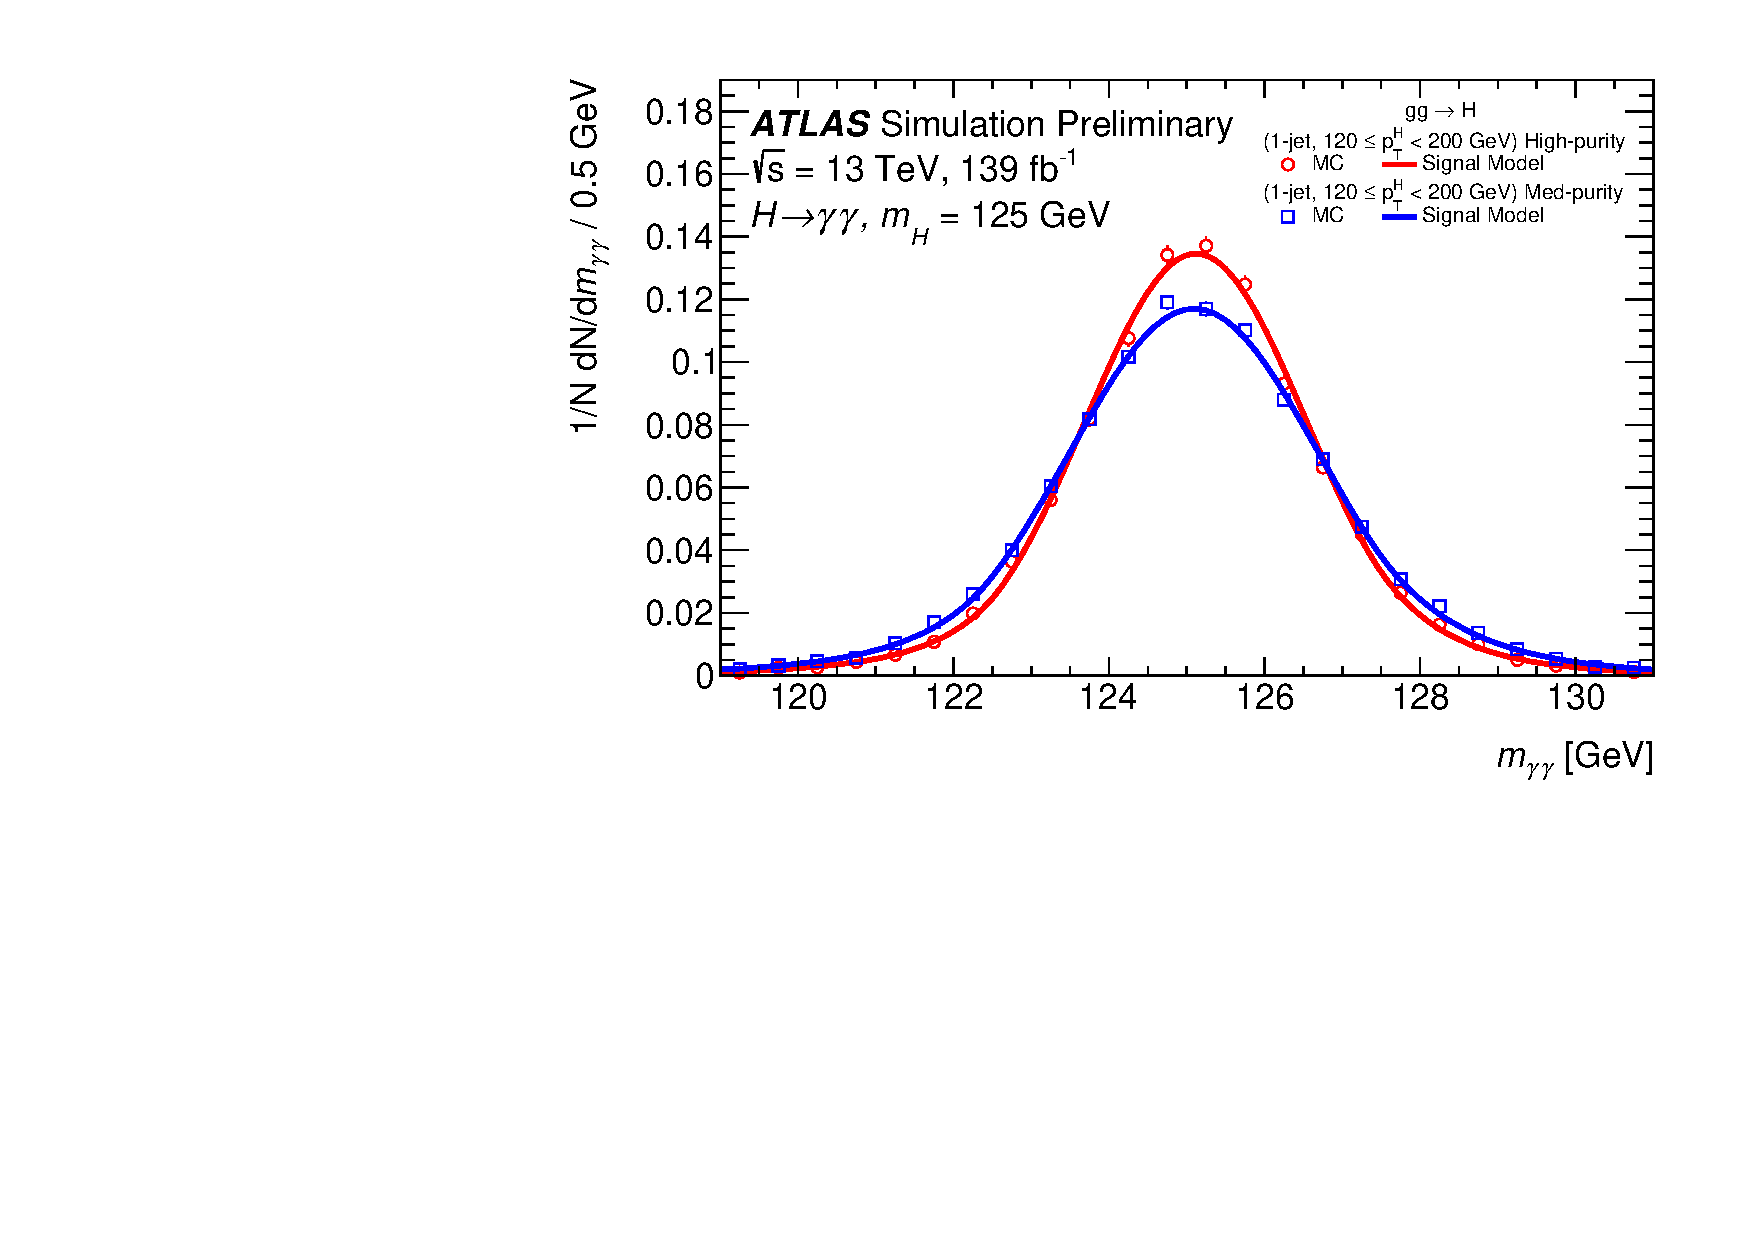
\includegraphics[width=0.49\textwidth]{figures/sigbkgparam/ggH_1J_120_200.pdf}\label{fig:DSCBgg2H}}
\subfloat[\ttH]{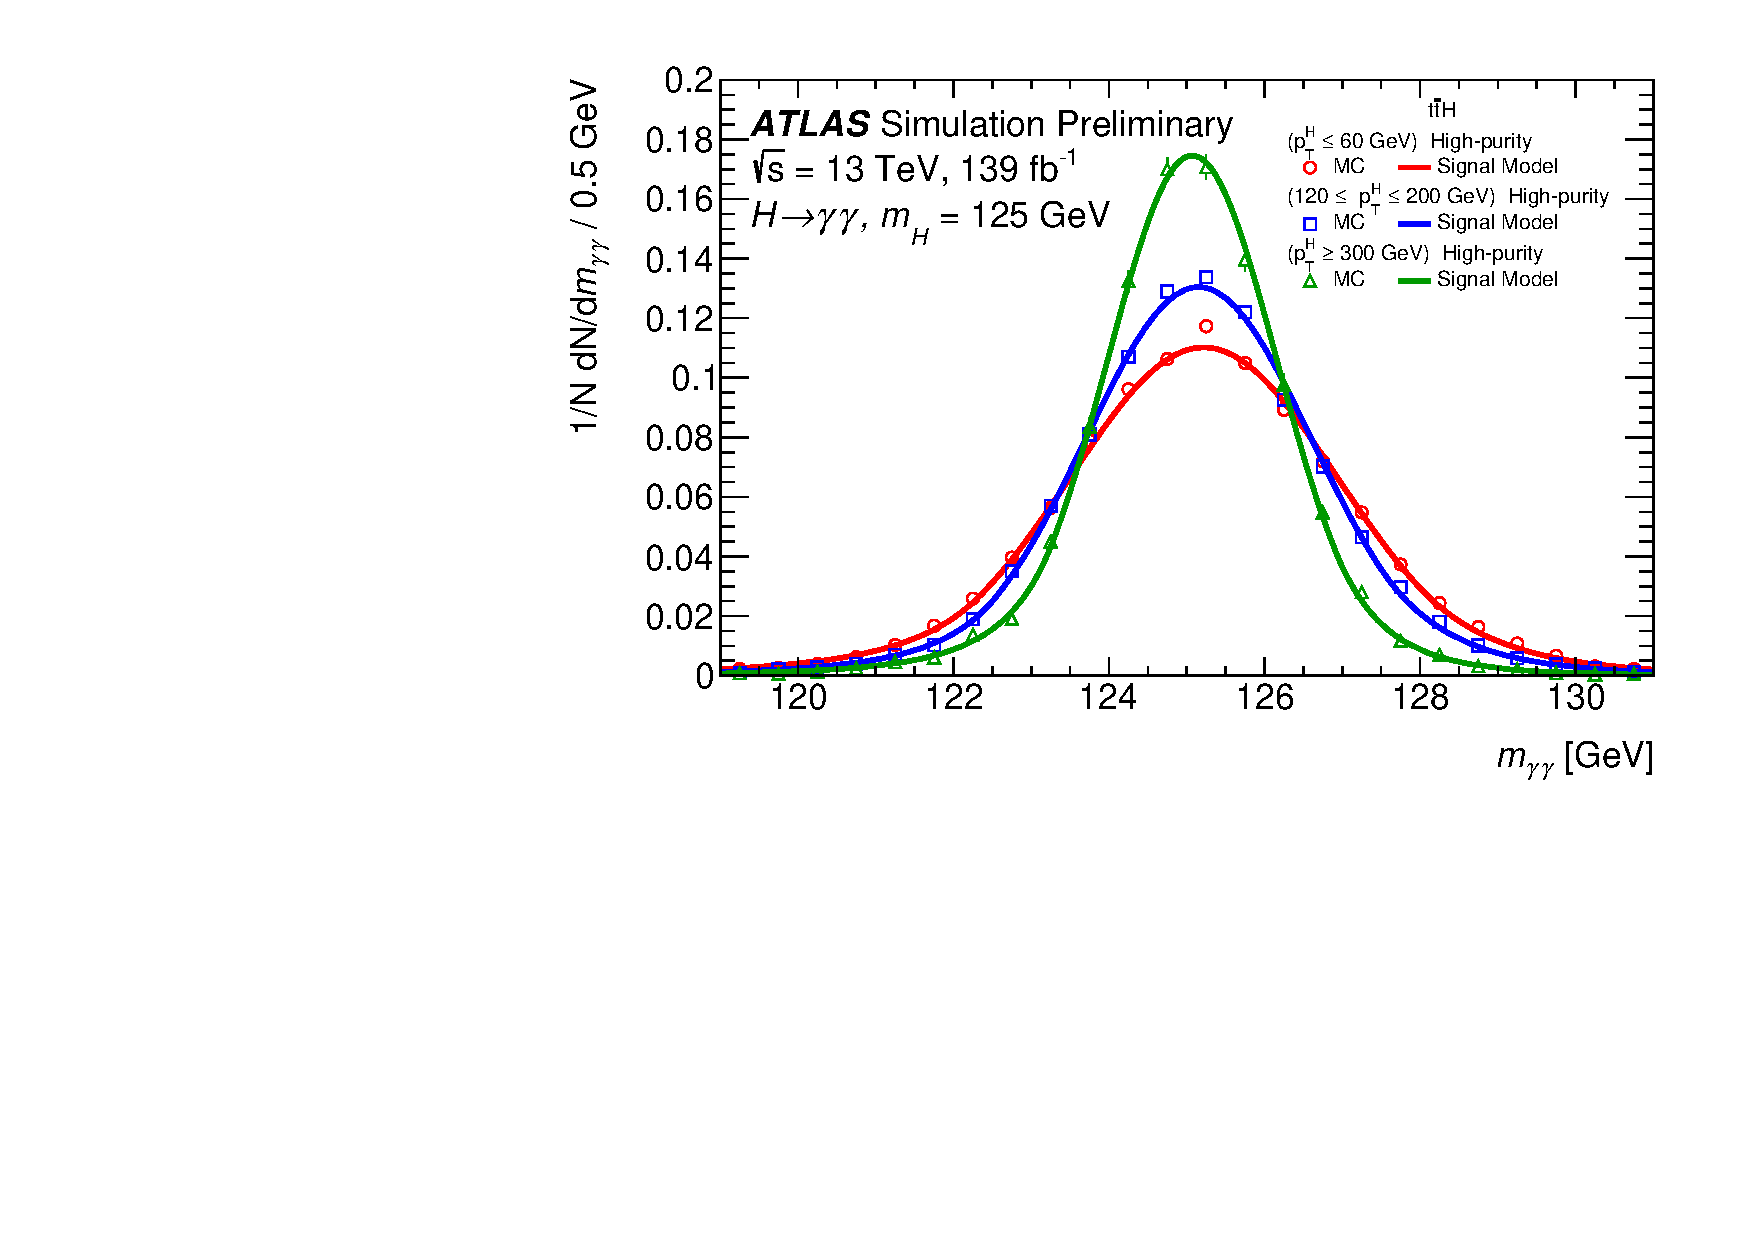
\includegraphics[width=0.49\textwidth]{figures/sigbkgparam/ttH.pdf}\label{fig:DSCBttH}}
\caption{DSCB shapes for two groups of categories. \ref{fig:modeling:signal:gg2H} depicts the signal shapes for two categories targeting the same STXS truth bin, one low-purity and one high-purity. \ref{fig:modeling:signal:ttH} depicts the signal shapes for three high-purity categories targeting different $p_{T}^{H}$ regions of the $ttH$ process.}
\label{fig:DSCB}
\end{figure}

\section{Background Modelling and Spurious Signal} \label{sec:background_modelling} 

Like the signal, the background is also parameterized as a smoothly-falling functional form in each category. This is done in a data-driven manner: first, a functional form is chosen using simulation-derived (or NTI-derived) templates to minimize the "spurious signal" systematic uncertainty. The background normalization and parameters of this functional form are then allowed to float in the final fit to the data, i.e., they are not fixed as a result of the spurious signal test. 

Background templates for the spurious signal test are constructed from Monte Carlo or NTI data to resemble the expected TI data as closely as possible in each category. The construction of the templates is detailed further in section \label{sec:bkgtemplates}.

The spurious signal test is a signal-plus-background functional fit to a background-only distribution. This provides a relatively simple way to measure background mismodelling- the background template contains no true Higgs signal, so the functional form that best models the background is the one for which the extracted "spurious" signal is closest to zero. This is illustrated in figure \ref{fig:SScartoon}. Spurious signal can be positive or negative- if positive, the functional form chosen "undershoots" the true background, while if negative, the functional form chosen "overshoots" the true background.

\begin{figure}
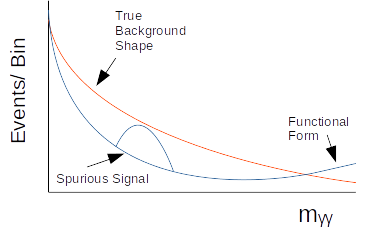
\includegraphics[width=0.49\textwidth]{figures/sigbkgparam/SSCartoon.png}
\caption{A cartoon depicting the spurious signal procedure. The true background shape in red is modeled by an analytic function in blue. The spurious signal resulting from this mismodelling is the maximum signal yield extracted from the blue "spurious signal" bump, fit over a window of $120 GeV < m_{\gamma \gamma}<130 GeV$.}
\label{fig:SScartoon}
\end{figure} 

The spurious signal fit is performed for signal masses from 121 GeV to 129 GeV at intervals of 1 GeV; the number of spurious signal events $N_{sp}$ is defined as the maximum of the absolute value of the number of signal events extracted from this range. The functional form chosen is one of the following functional forms:

\begin{itemize}
\item Exponential Function: $f(\myy) = e^{c\cdot \myy}$
\item Exponential Function of $2^{nd}$ Order Polynomial: $f(\myy) = e^{c_1\cdot m^2_{\gamma\gamma}+c_2\cdot \myy}$
\item Bernstein polynomial of order $N$: $B_{N}(\myy) = \sum_{i=0}^N c_i\cdot b_{i,N}$ with $b_{i,N} = \begin{pmatrix}N\\i\end{pmatrix}\myy^i (1-\myy)^{N-i}$
\item First-Order Power Law Function: $f(\myy) = \myy^c$
\end{itemize}

Functional forms chosen are then required to satisfy one of the two following criteria:

\begin{itemize}
\item $N_{s} < 0.1 \times N_{s,exp}$, where $N_{s,exp}$ is the expected true signal in a given category
\item $N_{s} < 0.2 \times \sigma_{s,exp}$, where $\sigma_{s,exp}$ is the statistical uncertainty on the expected true signal in a given category
\end{itemize}

If more than one function passes these criteria, the function with the lower number of degrees of freedom is selected. If there are multiple functions that pass the critera and have the same number of degrees of freedom, the function with the lowest resulting spurious signal is selected.

In low statistics categories, it is not uncommon that no functional form will satisfy the above criteria. In this case, the "relaxed" spurious signal fit is performed, which replaces $N_{s}$ with a new variable $\zeta_{s}$ that is designed to accomodate up to $2\sigma$ fluctuations in the spurious signal:

\[\zeta_{s} = \begin{cases} 
      N_{s} + 2 \delta_{MC} if  N_{s} + 2 \delta_{MC} < 0\\
      N_{s} - 2 \delta_{MC} if  N_{s} - 2 \delta_{MC} > 0\\
      0 otherwise \\
   \end{cases}
\]

Though $\zeta_{s}$ is used to define the spurious signal criteria, $N_{s}$ is still used for the final spurious signal uncertainty. 

\begin{figure}
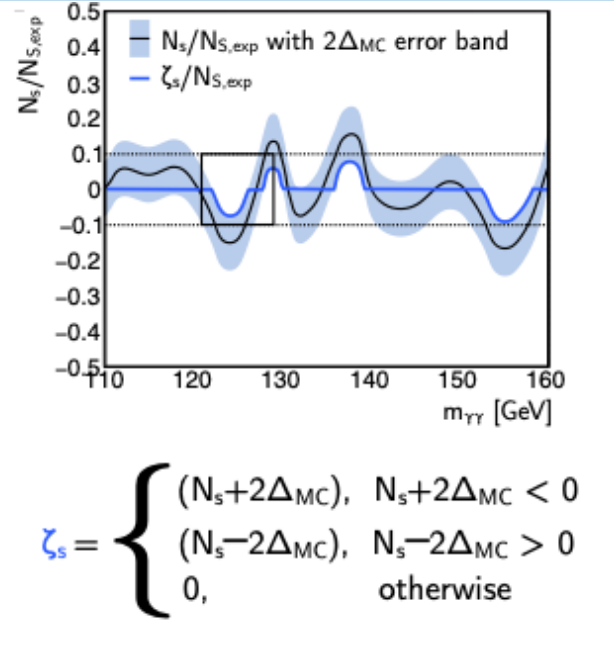
\includegraphics[width=\linewidth]{figures/sigbkgparam/SSRelaxed.png}
\caption{A cartoon depicting the "relaxed" spurious signal procedure. Two-sigma fluctuations of the background are incorporated into the spurious signal procedure in order to select a functional form.}
\label{fig:SSrelaxed}
\end{figure} 


An additional requirement that the $\chi^{2}$ probability of the signal-plus-background fit in the spurious signal test is greater than 1\% is applied in the Couplings analysis; while this is not a requirement in the CP analysis, all sprurious signal fits nonetheless satisfy this criterion as well.

In the Couplings analysis, several of the very low-stat categories nevertheless produce unphysical fits using these criteria. Thus, in categories of this analysis containing fewer than 100 events in the data sidebands, a Wald test is performed: the functional forms are restricted to Exp, ExpPoly2, and ExpPoly3, and their respective maximum-likelihoods $L_{1}$, $L_{2}$, and $L_{3}$ are computed from a fit to the TI data sidebands. The quantities $q_{ij} = -2 ln(\frac{L_{i}}{L_{j}})$ are then calculated and converted into p-values, assuming that $q_{ij}$ follows a $\chi^{2}$ distribution with one degree of freedom. If the p-value calculated is < 0.05, the function with the larger number of degrees of freedom is chosen. 

An illustration of the Wald test in two of the Couplings categories is shown in Figure \ref{fig:WaldTest}.

\begin{figure}
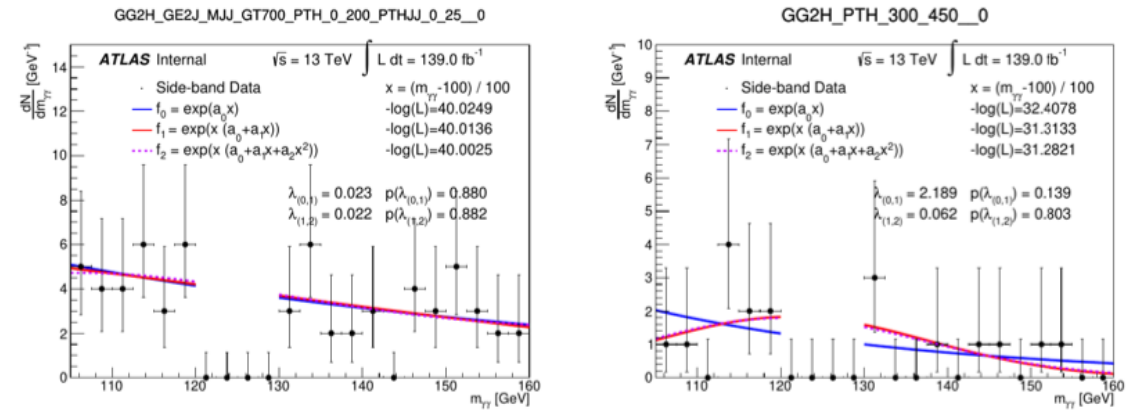
\includegraphics[width=\linewidth]{figures/sigbkgparam/Walds.png}
\caption{An example of the Wald test being performed in two low-statistics Couplings categories. The exponential functional form is chosen in both cases.}
\label{fig:WaldTest}
\end{figure} 

These failed fits show the limitations of current spurious signal criteria: in low-statistics categories, the Monte Carlo templates often contain large statistical fluctuations that can be fit as spurious signal. However, because spurious signal is intended to measure the mismodelling due to the choice of functional form, the presence of such fluctuations can artifically inflate the spurious signal. If the functional forms chosen because of these fluctuations have too many degrees of freedom, this can cause disastrous effects when fitting to the true data sidebands, as statistical fluctuations in data will dominate. This is the motivation for introducing Gaussian Process Regression (GPR) smoothing, discussed in appendix \ref{sec:gpr}. At the time of this writing, this novel smoothing procedure is currently being implemented in the Coupling analysis; a discussion of the procedure and the improvements to the spurious signal that result are given in appendix \ref{sec:gpr}, while extensive validation of the smoothing procedure using toy tests is given in appendix \ref{sec:gpr_validation}.

\subsubsection{Background Templates} \label{sec:bkgtemplates} 

The background templates constructed for both analyses discussed in this dissertation are designed to approximate the continuum diphoton background. 

In all categories of the CP analysis, either $tt\gamma\gamma$ Monte Carlo or NTI data is used to model the continuum background, scaled to the TI data sidebands. The statistical uncertainty of both template candidates is checked in each region by taking the integral and sum of errors; the template chosen is the one with the smallest statistical uncertainty. $tt\gamma\gamma$ is ultimately used to construct the template in all CP analysis categories but one. 

Similarly, in the leptonic $VH$ categories of the Coupling analysis, a combination of $\gamma\gamma + V\gamma\gamma$ Monte Carlo, scaled to match the TI sidebands, is used. However, in the other $ggH$ and $VBF$ categories, a more sophisticated data-driven method is used due to the nontrivial presence of fake photons arising from misidentified jets. 

First, the purity fraction, i.e. the fraction of true vs. fake diphoton events in data, is calculated in each category. This is done using a double two-dimensional ABCD method \cite{purity1} \cite{purity2}.

For a given choice of photon (either leading or subleading) four regions are constructed in each category:

\begin{itemize}
\item Region A, in which the photon passes the Tight ID criterion and the Tight isolation criterion
\item Region B, which the photon passes the Tight ID criterion and fails the Tight isolation criterion
\item Region C, in which the photon fails the Tight ID criterion (but passes the LoosePrime3 ID criterion) and fail the Tight isolation criterion
\item Region D, in which the photon fails the Tight ID criterion (but passes the LoosePrime3 ID criterion) and passes the Tight isolation criterion
\end{itemize} 

Assuming that the ID and isolation cuts are independent with $\epsilon_{ID}$ and $\epsilon_{iso}$, and that the photons in all regions but region A are definitively fakes, it is possible to define the number of fake photons in region A as:

\begin{equation}
N_{A} = \epsilon_{iso} N_{B} = \epsilon_{ID} N_{D} = \epsilon_{iso} \epsilon_{ID} N_{C}
\end{equation} 

Extending this to the diphoton pair, eight total regions can be defined in each category, allowing us to quantify the ($\gamma \gamma / \gamma j/jj$) fraction in each category. However, the assumption that the isolation and ID cuts are independent is not strictly valid, so it is not enough to perform a simple counting-experiment to determine the fraction of jets: various correlation terms must be considered, so a fit must be performed. The fit has sixteen equations with nineteen variables, and is performed following the process in \cite{purity1} and \cite{purity2}.

After the purity fractions are calculated in each category, the shapes of the $\gamma j$ and $jj$ distributions are derived using NTI data. The $\gamma \gamma$ Monte Carlo is then reweighted to match these shapes, and the $\gamma \gamma$, $\gamma j$, and $jj$ contributions are added according to their purities. As in other categories, the templates are scaled to the TI sidebands. 

\section{Likelihood Fitting and Asimov Data} \label{sec:likelihoodfit} 

The fits performed in all analyses discussed in this dissertation use a test statistic called a Profile Likelihood Ratio. The likelihood ratio  is a Bayesian variable that is simply defined as $\mathcal{L}(\vec{x},\vec{\theta}) = P(\vec{x} | vec{\theta})$  for a set of observed data points $\vec{x}$ and a set of additional nuisance-parameter variables $\vec{theta}$ such as background normalization, shape, and systematic uncertainties \cite{Cowan}.

For independent, identically distributed Poisson variables (i.e., the number of signal and background events in a given histogram bin $i$), we can parameterize the likelihood as:

\begin{equation}
\mathcal{L}(\mu, N_{b}, \vec{zeta}) = \prod_{i}^{N}{\frac{(\mu \times s_{i}+ N_{b} \times b_{i}(\vec(\zeta)))^{n_{i}} \times e^{-(\mu \times s_{i}+ N_{b} \times b_{i}(\vec(\zeta))) }}{n_{i}!}}
\end{equation}

for signal strength $\mu$, expected signal and background probability distributions $s_{i}$ and $b_{i}$ in each bin, nuisance parameters $\vec{\theta} = (N_{b}, \vec{\zeta})$ governing the total background normalization and shape, and $n_{i}$ observed number of events in bin i. Likelihoods can also be constructed in an unbinned manner by taking the continuous form of $s_{i}$ and $b_{i}$ as a function of $m_{\gamma\gamma}$. For a multi-category analysis, the total likelihood is taken as the product of the likelihood in each category.

Using this, we can construct the Profile Likelihood Ratio as: 
\begin{equation}
\lambda(\mu) = \frac{\mathcal{L}(\mu, \hat{\hat{\theta}}(\mu))} {\mathcal{L}(\hat{\mu}, \hat{\theta}}
\end{equation}

where $\hat{\hat{\theta}}(\mu)$ is the set of values of $\vec{theta}$ that conditionally maximize $\mathcal{L}$ for each given $\mu$, and $\hat{\theta}, \hat{\mu}$ are the values of $\vec{theta}$ and $\mu$ that maximize $\mathcal{L}$ globally.

By maximizing $\lambda$, or, more commonly, by minimizing $-2ln(\lambda)$ (due to its comparative ease of computation) it is possible to extract a best-fit value for $\mu$ given a set of data. By definition, $\mu$ is the ratio of the observed signal yield to the one expected in the SM; however, it is also possible to parameterize $\mu$ in terms of other variables, such as the various $\kappa$ couplings. This parameterization is performed in both analyses dicussed in this dissertation, and is detailed further in \ref{chap:tthcpresults} and \ref{chap:couplingsresults}.

Systematic uncertainties enter into the fit as nuisance parameters. In order to treat additional systematic uncertainties on the signal shape and yield in a manner similar to the treatment of the systematic uncertainties on the background, the Double-Sided Crystal Ball parameters $\mu_{CB}$ and $\sigma_{CB}$ that enter into the parameterization of $s_{i}$ are modified by energy scale and resolution shifts of magnitude $\sigma$ and sign $\theta$:

\begin{equation}
\mu_{CB} = \mu_{CB} \prod_{k} (1+\sigma_{ES,k}\theta_{ES,k}) 
\end{equation}
\begin{equation}
\sigma_{CB} = \sigma_{CB} \prod_{j} (1+\sigma_{ER,j}\theta_{ER,j}) 
\end{equation}

Similar response-term modifications can be performed to the luminosity and trigger uncertainties affecting overall signal yield. Additional constraint terms (given a Gaussian, Log-Normal, or Asymmetric \cite{Cranmer}) that are equivalent to the Bayesian prior distribution for each nuisance parameter are also multiplied to the total likelihood, in order to correctly model their allowed spread \cite{JSConway}.

When performing a likelihood fit, it is often useful to construct a representative "Asimov" dataset generated by fixing both $\mu$ and particular nuisance parameters.

Pre-fit Asimov data is constructed by performing an unbinned, background-only profile likelihood ratio fit to the TI sidebands. The nuisance parameters are then set to the values extracted from this fit, and a Standard Model signal with significance $\mu = 1$ (that is, exactly corresponding to the predicted signal yield) is then superimposed atop the background shape. Similarly, after unblinding the signal region, post-fit Asimov data is constructed by fitting to the entire dataset, extracting the values for the nuisance parameters, and again superimposing a Standard Model signal with significance $\mu = 1$ atop the background. The reason for constructing both pre-fit and post-fit Asimov is to evaluate the "pull" of various nuisance parameters based on the data in the signal region: if the fit after including signal-region data causes a nuisance parameter to deviate substantially from the norm, it is possible that one or more systematics are not well-modelled.

The list of systematic uncertainties and the expected significances derived from pre- and post- fit Asimov data for both analyses discussed in this dissertation are given in Chapters \ref{chap:tthcpresults} and \ref{chap:couplingsresults}.
 

\chapter{Study of the CP Properties of the Top Quark Yukawa Interaction in $t\bar{t}H$ and $tH$ Events with $H \rightarrow \gamma \gamma$: Selection and Categorization} \label{chap:tthcp_chapter}
	\section{Study of the CP properties of the top-quark Yukawa interaction in t\bar{t}H and tH events wth H \rightarrow \gamma \gamma} \label{sec:ttHCPCategorization}

In order to properly measure the dependence of the top Yukawa coupling on the CP-mixing angle $\alpha$, we divide a region of $ttH$-and-$tH$-enriched phase space into a number of different categories based both upon the similarity of events it contains to signal (Higgs processes like $ttH$ and $tH$) rather than background (non-Higgs continuum diphoton processes), as well as the similarity of events it contains to CP-odd rather than CP-even Higgs processes. By creating many such categories and fitting the event yield in each, we can set detailed constraints on the value of $\alpha$.

First, we define two sets of regions. The "hadronic" region targets events containing fully-hadronic top decays, requiring two loose-ID photons, one b-tagged jet at the 77\% working point with p_{T} > 25 GeV, as well as two additional jets with p_{T} > 25 GeV and exactly zero electrons or muons. Similarly, the "leptonic" region targets events containing semi-leptonic top decays, requiring two loose-ID photons, one b-tagged jet at the 77\% working point with p_{T} > 25 GeV, as well as at least one isolated electron or muon.

To perform the categorization in these regions, two multivariate Boosted Decision Trees (BDTs) are used, one to separate Higgs events from background and one to separate CP-odd Higgs events from CP-even Higgs events. Both BDTs are trained on low-level kinematic features using the XGBoost package \ref{cite:XGBoost}.

\subsection{SBBDT}

The signal-versus-background BDT (SBBDT) developed for use in the CP Analysis is identical to that developed first in the $79.8 fb^{-1}$ measurements of $ttH$ in the diphoton channel \ref{cite:ATLAS-CONF-2019-004} in and later retrained for $139 fb^{-1}$ measurements of $ttH$ in the diphoton channel \ref{cite:ATLAS-CONF-2019-004}. It is trained separately for both the hadronic and leptonic regions.

Both the hadronic and leptonic BDTs are trained using a Standard-Model Powheg $ttH$ Monte Carlo sample to model the signal and NTI data control events to model the continuum diphoton background.

\subsubsection{Hadronic Region} \label{sec:SBBDThad} 
In the hadronic region, 60\% of the $ttH$ Monte Carlo signal events are used for training, 20\% are reserved for categorization and BDT hyperparameter optimization, and the final 20\% are reserved for validation. 60\% of the NTI events are used for training, 20\% are reserved for hyperparameter optimization, and the remaining 20\% are reserved for testing.

The input variables chosen are: 

\begin{itemize}
\item $p_T/m_{\gamma \gamma}$, $\eta$ and $\phi$ of the two photons. Photon $p_{T}$ is scaled by $m_{\gamma \gamma}$ to reduce unwanted sculpting of the diphoton mass spectrum. 
\item $p_T$, $\eta$, $\phi$ and E of the six jets with highest $p_{T}$
\item Boolean b-tag flag (77\% working point) for each of the six jets with highest $p_{T}$
\item \MET and direction of \MET
\end{itemize}

Distributions of the BDT input variables using $79.8 fb^{-1}$ of data are shown in figures XXX through XXX.

\subsubsection{Leptonic Region} \label{sec:SBBDTlep} 

As in the hadronic region, in the leptonic region, 60\% of the $ttH$ Monte Carlo signal events are used for training, 20\% are reserved for categorization and BDT hyperparameter optimization, and the final 20\% are reserved for validation. 75\% of the NTI events containing zero b-jets but at least one un-tagged jet wiare used for training and the remaining 25\% are reserved for hyperparameter optimization, while 50\% of the NTI events containing one or more b-jets are used for categorization and the remaining 50\% are reserved for testing.

However, due to lower statistics in the leptonic top decay channel due to the smaller top-quark branching ratio to leptons, two cuts are relaxed for the development of the leptonic BDT:

\begin{itemize}
\item The relative $p_{T}$ cuts are loosened from $\frac{p_{T}}{m_{\gamma\gamma} > 0.35$ for the leading photon and $\frac{p_{T}}{m_{\gamma\gamma} > 0.25$ for the subleading photon to a flat $p_{T} > 35$ GeV for the leading photon and $p_{T} > 25$ GeV for the subleading photon.
\item The diphoton invariant mass window is extended from $105 GeV < m_{\gamma \gamma} < 160 GeV$ to $80 GeV < m_{\gamma \gamma} < 250 GeV$.
\end{itemize}

The cuts are again tightened to define the signal region after BDT training is complete- that is, the loosening of these cuts is only utilized to increase BDT training statistics, and does not carry through to other stages of the analysis.

The input variables chosen are: 

\begin{itemize}
\item $p_T/m_{\gamma \gamma}$, $\eta$ and $\phi$ of the two photons. Photon $p_{T}$ is scaled by $m_{\gamma \gamma}$ to reduce unwanted sculpting of the diphoton mass spectrum.
\item $p_T$, $\eta$ and $\phi$ of up to two leptons. 
\item $p_T$, $\eta$, $\phi$ and E of the four jets with highest $p_{T}$
\item Boolean b-tag flag (77\% working point) for each of the four jets with highest $p_{T}$
\item \MET and direction of \MET
\end{itemize}

Distributions of the BDT input variables using $79.8 fb^{-1}$ of data are shown in figures XXX through XXX.

The BDT output distributions are shown in figures XXX through XXX.

We note that the SBBDT performance is independent of $\alpha$; this can be seen in figures XXX through XXX.

\subsection{CP-Sensitive Observables}

In order to train a BDT to discriminate between CP-even and CP-odd $ttH+tH$, we must plot variables at truth-level and investigate their dependence on $\alpha$. We use the HC model $ttH$ and $tH$ samples with alternative values of $\alpha$ generated using MadGraph5_aMCatNLO, added according to their calculated cross-sections given in table XXX.

From these plots, we observe that the strongest variable is the Higgs boson $p_{T}$ : CP-odd $ttH$ and $tH$ have a much more boosted Higgs than CP-even $ttH$ and $tH$, and are more central in $\eta$. Similarly, the angular separation $\Delta \eta$ between the top and anti-top is much larger in CP-odd $ttH$, while the top and anti-top are more back-to-back in azimuthal angle $\Delta \phi$ in CP-even $ttH$ than in CP-odd $ttH$. In $tHjb$ events, we note that the top $p_{T}$ and $\eta$ also have discriminatory power. The mass of the Higgs + leading top system also offers discriminatory power- for $ttH$ and $tWH$ events it increases with $\alpha$, while for $tHjb$ events it decreases with $\alpha$ .

These variables are shown in Figures XXX through XXX.










 

\chapter{Study of the CP Properties of the Top Quark Yukawa Interaction in $t\bar{t}H$ and $tH$ Events with $H \rightarrow \gamma \gamma$: Results} \label{chap:tthcp_results}
	Following the categorization in the previous chapter, a measurement of the CP-mixing term in the top Yukawa coupling is performed. 

\section{Yield Dependence on $\alpha$} \label{sec:YieldPar}

In order to perform a measurement of the parameters $\alpha$ and $\kappa_{t}$, the yield in each category must be parameterized as a function of these parameters. This takes the same form as cross-section dependence:

\begin{equation}
y_{i}^{ttH} =  A_{i}\kappa_{t}^{2} (cos(\alpha)^{2}) + B_{i}\kappa_{t}^{2} (sin(\alpha)^{2}) + E_{i} \kappa_{t}^{2} cos(\alpha)sin(\alpha)
\end{equation}

for some constants A, B, and E (with E expected to be close to zero for $ttH$), while the $tWH+tHjb$ yield can be parameterized as:

\begin{equation}
y_{i}^{tH} =  A_{i}\kappa_{t}^{2} (cos(\alpha)^{2}) + B_{i}\kappa_{t}^{2} (sin(\alpha)^{2}) + C_{i}\kappa_{t} (cos(\alpha))+ D_{i}\kappa_{t} (sin(\alpha)) + E_{i} \kappa_{t}^{2} cos(\alpha)sin(\alpha) + F_{i}
\end{equation}

for different constants A, B, C, D, E and F. A-terms correspond to the CP-even contribution to the $t-H$ coupling, B-terms correspond to the CP-odd contribution to the $t-H$ coupling, E-terms correspond to the interference between the CP-even and the CP-odd contribution to the $t-H$ coupling, C-terms correspond to the interference between the CP-even contribution to the $t-H$ coupling and the purely Standard Model $W-H$ coupling, D-terms correspond to the interference between the CP-odd contribution to the $t-H$ coupling and the purely Standard Model $W-H$ coupling, and F-terms correspond to purely Standard Model $W-H$ coupling alone.

These constants are determined by fitting the yield in each category using the Monte Carlo samples generated for a variety of $\alpha$ points. Because of a degeneracy in the A, B, and F coefficients of the $tH$ yield, it is also necessary to use samples with $\kappa_{t} \neq 1$ to determine the coefficients. The parameterizations of the total inclusive yields as a function of $\alpha$, and the coefficients for each category, are shown in figure \ref{fig:ttHYield} for $ttH$, \ref{fig:tWHYield} for $tWH$ and \ref{fig:tHjbYield} for $tHjb$.

\begin{figure}[htp]
  \centering
       \begin{subfigure}[b]{0.3\textwidth}
         \centering
         \includegraphics[width=\textwidth]{figures/tthcp_results/yield_ttH_0.pdf}
         \caption{$ttH$}
         \label{fig:ttHYield}
     \end{subfigure}
     \hfill
         \begin{subfigure}[b]{0.3\textwidth}
         \centering
         \includegraphics[width=\textwidth]{figures/tthcp_results/yield_tWH_0.pdf}
         \caption{$tWH$}
      \label{fig:tWHYield}
     \end{subfigure}
     \hfill 
        \begin{subfigure}[b]{0.3\textwidth}
         \centering
         \includegraphics[width=\textwidth]{figures/tthcp_results/yield_tHjb_0.pdf}
         \caption{$tHjb$}
         \label{fig:tHjbYield}
     \end{subfigure}
     \hfill
  \label{fig:YieldParams}
  \caption{Inclusive yield parametrizations as a function of $\kappa_{t}$ and $\alpha$, normalized to $139 fb^{-1}$.}  
\end{figure}


The $ggF$ cross-section and $H \rightarrow \gamma \gamma$ branching ratio can also be parameterized in terms of $kappa_{t}$ and $\alpha$; this is detailed more in section \ref{sec:results}

\section{Signal and Background Parameterization}

The signal and background shapes are parameterized according to the prescription in \ref{sec:sigbkgparam}, using a Double-Sided Crystal Ball function for the signal shape and following the spurious signal test procedure for the background parameterization. The DSCB shape does not vary noticeably with $\alpha$, so the Standard-Model Higgs signal DSCB parameterization is used for all $\alpha$ variations occurring in the analysis.

In all categories but one, the $tt\gamma\gamma$ Monte Carlo sample is used for the background template. However, in Hadronic Category 10, a fluctuation in the Monte Carlo causes the spurious signal test to fail- in this category, we choose NTI data as the source of the template due to its lower statistical uncertainty. DSCB parameterizations are given in Tables \ref{tab:sig_param1}-\ref{tab:sig_param2} , while the spurious signal values, template source, choice of functional forms, and fit $\chi^{2}$ probability are shown in Table \ref{tab:spuriousSignal_1}. $Z_{sp}$ denotes the max spurious signal over the statistical uncertainty on the background, while $\mu_{sp}$ denotes the max spurious signal over the expected signal yield in that category.

\begin{table}[!htp]
\begin{center}
\begin{tabular}{lrr}
        \hline
        {} & $\mu_{CB}$ [GeV] & $\sigma_{CB}$ [GeV]  \\
        \hline
        1 & 125.100 & 1.157 \\
        2 & 125.121 & 1.345 \\
        3 & 125.269 & 1.635 \\
        4 & 125.132 & 1.206 \\
        5 & 125.173 & 1.499 \\
        6 & 125.169 & 1.635 \\
        7 & 125.091 & 1.207 \\
        8 & 125.177 & 1.580 \\
        9 & 125.205 & 1.724 \\
        10 & 125.100 & 1.290  \\
        11 & 125.148 & 1.546 \\
        12 & 125.206 & 1.697 \\ \hline

        13 & 125.109 & 1.293 \\
        14 & 125.174 & 1.608 \\
        15 & 125.153 & 1.454 \\
        16 & 125.186 & 1.704 \\
        17 & 125.200 & 1.705 \\
        18 & 125.030 & 1.684 \\
        19 & 125.173 & 1.759 \\
        20 & 125.143 & 1.784 \\
        \hline
\end{tabular}
\caption{Best-fit parameter values for the Gaussian core of the DSCB in each analysis category.}
\label{tab:sig_param1}
\end{center}
\end{table}

\begin{table}[!htp]
\begin{center}
\begin{tabular}{lrrrr}
        \hline
        {} & $\alpha_{CB}^\text{low}$ & $\alpha_{CB}^{high}$ & $n_{CB}^\text{low}$ & $n_{CB}^{high}$ \\
        \hline
        1 & 1.616 & 1.484 & 6.226 & 15.519 \\
        2 & 1.752 & 1.456 & 4.127 & 15.476 \\
        3 & 1.715 & 1.719 & 4.516 & 11.878 \\
        4 & 1.583 & 1.530 & 4.782 & 5.702 \\
        5 & 1.660 & 1.481 & 6.853 & 15.048 \\
        6 & 1.611 & 1.420 & 8.027 & 35.892 \\
        7 & 1.615 & 1.494 & 5.570 & 11.610 \\
        8 & 1.619 & 1.700 & 5.801 & 7.585 \\
        9 & 1.710 & 1.676 & 4.356 & 12.189 \\
        10 & 1.804 & 1.597 & 13.580 & 7.932 \\
        11 & 1.700 & 1.594 & 4.740 & 7.589 \\
        12 & 1.531 & 1.530 & 8.478 & 13.347\\ \hline
        13 & 1.597& 1.546 & 6.806 & 11.117\\
        14 & 1.659 & 1.549 & 5.237 & 15.030\\
        15 & 1.600 & 1.633 & 5.741 & 5.970\\
        16 & 1.691 & 1.698 & 6.650 & 14.434 \\
        17 & 1.534 & 1.460 & 7.863 & 14.413 \\
        18 & 1.848 & 1.606 & 18.705 & 12.706 \\
        19 & 2.150 & 1.505 & 1.432 & 10.219\\
        20 & 1.553 & 1.578 & 10.752 & 14.703\\
        \hline
\end{tabular}
\caption{Best-fit parameter values for the exponential tails of the DSCB in each analysis category.}
\label{tab:sig_param2}
\end{center}
\end{table}


\begin{table}[ht]
  \centering
  \begin{tabular}{l l l c c c c c c c c c c c}
    \hline
    Category & Template Process & Function & $Z_{sp}$ [\%] &  $Z_{sp}^\text{relax}$ [\%] & $\mu_{sp}$ [\%] & $\mu_{sp}^\text{relax}$ [\%] & $N_{sp}$ & Prob($\chi^2$)\\ \hline
1 & $tt+\gamma\gamma$ & Exponential & 28.5 & 0 & 15 & 0 & 0.426 & 90\\
2 & $tt+\gamma\gamma$ & Power Law & -14.2 & 0 & -6.75 & 0 & -0.297 & 82\\
3 & $tt+\gamma\gamma$ & Exponential & 19.6 & 1.83 & 14.9 & 1.43 & 0.26 & 3\\
4 & $tt+\gamma\gamma$ & Exponential & 22.3 & 0 & 35.7 & 0 & 0.311 & 74\\
5 & $tt+\gamma\gamma$ & Power Law & -21.9 & 0 & -32.3 & 0 & -0.566 & 29\\
6 & $tt+\gamma\gamma$ & Exponential & 14.7 & 0 & 18.4 & 0 & 0.335 & 94\\
7 & $tt+\gamma\gamma$ & Exponential & 35.4 & 0 & 90.9 & 0 & 0.644 & 1\\
8 & $tt+\gamma\gamma$ & Exponential & -28.6 & 0 & -47.7 & 0 & -1.23 & 85\\
9 & $tt+\gamma\gamma$ & Power Law & -9.45 & 0 & -12.2 & 0 & -0.264 & 79\\
10 & NTI & Power Law & -89.5 & 0 & -1180 & -8.09 & -1.31 & 62\\
11 & $tt+\gamma\gamma$ & Exponential & 79 & 0 & 324 & 0 & 4.5 & 26\\
12 & $tt+\gamma\gamma$ & Exponential & 28.8 & 0 & 45 & 0 & 3.05 & 48\\ \hline
13 & $tt+\gamma\gamma$ & Exponential & 18 & 0.852 & 5.04 & 0.246 & 0.199 & 48\\
14 & $tt+\gamma\gamma$ & Exponential & 7.17 & 0 & 3.35 & 0 & 0.129 & 46\\
15 & $tt+\gamma\gamma$ & Power Law & -17.1 & 0 & -19.9 & 0 & -0.205 & 39\\
16 & $tt+\gamma\gamma$ & Exponential & 15.5 & 0 & 19.3 & 0 & 0.398 & 66\\
17 & $tt+\gamma\gamma$ & Power Law & -22 & -5.22 & -17.4 & -4.27 & -0.393 & 12\\
18 & $tt+\gamma\gamma$ & Exponential & 43.2 & 1.85 & 319 & 16.5 & 0.761 & 57\\
19 & $tt+\gamma\gamma$ & Power Law & -25.5 & 0 & -117 & 0 & -0.498 & 81\\
20 & $tt+\gamma\gamma$ & Exponential & 5.97 & 0 & -19.8 & 0 & -0.135 & 90\\ \hline
    \hline
  \end{tabular}
  \caption{Results of the spurious signal test for the analysis categories.}
  \label{tab:spuriousSignal_1}
\end{table}

\section{Systematic Uncertainty}

Uncertainties can effect both the overall yield of a given physics process and the migration of events between categories. For non-top Higgs processes (excluding $ggF$), only the uncertainties on the overall yield are calculated; however, for $ttH$, $tWH$, $tHjb$, and $ggF$, several migration uncertainties are accounted for as well.

\subsection{Theory Systematics}

Theory systematic uncertainties are designed to account for the precision (or imprecision) of the knowledge with which the models used in the analysis are constructed. These take on a number of different forms, including uncertainties on the parton distribution functions (PDFs), uncertainties on the QCD renormalization and factorization scale, and mismodelling of processes containing final-state b-jets.

QCD Renormalization Scale and Factorization Scale uncertainties are both calculated by varying the relevant QCD scale up or down by a factor of two in the Monte Carlo generator, while the PDF and strong coupling constant $\alpha_{s}$ uncertainties are calculated by varying the parameters according to the relevant LHAPDF \cite{LHAPDF} or PDF4LHC \cite{PDF4LHC} prescriptions.

Inclusive parametrization of the QCD and PDF uncertainties on a given process can be used when the effects of category migration are expected to be negligible. The inclusive parameterization of the QCD and PDF uncertainties on non-top Standard Model Higgs processes ($VBF$, $WH$, $ZH$ and $bbH$) is taken from \cite{YellowReport4}. However, previous analyses (\cite{HFunc1} \cite{HFunc2} \cite{HFunc3}) have shown that  processes containing final-state b-jets are poorly-modelled even after applying these yield uncertainties, so we apply a conservative 100\% uncertainty on the yield of $VBF$, $WH$, $ZH$ and $ggF$ in our analysis. This 100\% heavy-flavor uncertainty is not applied to $bbH$ due to its negligible contribution to the overall signal yield in the targeted analysis categories.

Similarly, the underlying event and parton showering uncertainties (UEPS) governed by the choice of MC showering tool are chosen by utilizing the Monte Carlo samples generated with the Herwig7 \cite{Herwig} showering tool rather than the Pythia8 tool \cite{Pythia8}. The uncertainty is given by:

\begin{equation}
UEPS= \frac{n_{Herwig}-n_{Pythia}}{n_{Pythia}}
\end{equation}

for each process in each category.

Similarly, a Monte Carlo generator uncertainty is calculated for $ttH$ and $ggH$ by comparing the Madgraph5\_aMC@NLO and Powheg samples.

Finally, an additional nuisance parameter is included to account for the theoretical uncertainty on the $H \rightarrow \gamma \gamma$ branching ratio. The number of nuisance parameters corresponding to each of the theoretical uncertainties and the form of the constraint term for each is given in Table \ref{tab:theorysyst}.

\begin{table}[ht]
\begin{center}
\begin{tabular}{lccccc}
\hline
Source & Number of NPs & Constraint type \\ \hline
$ttH$ QCD scale & 1 & log normal \\
$ttH$ PDF+$\alpha_S$ & 1 & log normal \\
$ttH$ UEPS & 1 & log normal \\
$ttH$ hard-process generator & 1 & log normal \\ \hline
$tHjb$ QCD scale& 1 & log normal \\
$tHjb$ PDF+$\alpha_S$ & 1 & log normal \\
$tHjb$ UEPS & 1 & log normal \\ \hline
$tWH$ QCD scale& 1 & log normal \\
$tWH$ PDF+$\alpha_S$ & 1 & log normal \\
$tWH$ UEPS & 1 & log normal \\ \hline
$ggH$ UEPS & 1 & log normal \\
$ggH$ hard-process generator & 1 & log normal \\
$bbH$ YR4 QCD scale & 1 & asymmetric \\
$bbH$ YR4 PDF + $\alpha_S$ & 1 & asymmetric \\
Non-top Heavy Flavor & 3 ($ggH$, $VBF$, $VH$) & log normal \\
$H\rightarrow\gamma\gamma$ BR & 1 & asymmetric \\
\hline
\end{tabular}
\end{center}
\vspace{-0.5cm}
\caption{A summary of the theory uncertainties used in the likelihood model.}
\label{tab:theorysyst}
\end{table}

\subsection{Experimental Systematics}

Due to the complexity of reconstructing physics objects, a large number of experimental systematics must also be calculated.
These include:

\begin{itemize}
\item Beam luminosity uncertainty \cite{ATLAS-CONF-2019-021}
\item Trigger uncertainty \cite{trigger} \cite{triggerperformance}
\item Pileup reweighting
\item Jet uncertainties: energy scale, energy resolution,  flavor-tagging and flavor composition \cite{jetuncs} \cite{jetuncs} \cite{jetuncs} \cite{jetuncs}
\item Photon uncertainties: energy scale and resolution (which modify the DSCB parameters as per Chapter \ref{chap:sigbkgparam}), photon ID, photon isolation \cite{CERN-EP-2019-145} \cite{photuncs}
\item Electron/muon uncertainties: energy scale, energy resolution, electron/muon ID, electron/muon isolation \cite{CERN-EP-2019-145} \cite{photuncs} \cite{elID-CERN-EP-2018-273} \cite{CERN-EP-2016-033}
\item MET uncertainties: \cite{MET1} \cite{MET2}
\item Higgs mass: \cite{Higgsmass}
\item Background modelling uncertainty: Calculated from spurious signal procedure discussed in Chapter \ref{chap:sigbkgparam}
\end{itemize}

Due to the number of experimental uncertainties considered, a merging scheme is adopted for photon energy scale and resolution systematics to take advantage of similar energy scale and resolution in certain regions of the detector.

The list of theoretical uncertainties and the form of the constraint term for each is given in Table \ref{tab:expsyst}.

\begin{table}[ht]
\begin{center}
\begin{tabular}{lccccc}
\hline
Source & Number of NPs & Constraint type \\ \hline
Yield \\ \hline
Luminosity & 1 & log normal  \\
Photon efficiency & 3 (ID, isolation, trigger) & asymmetric \\
\hline
Yield and Migration \\ \hline
Flavor tagging & 12 & asymmetric \\
Jets & 25 & asymmetric \\
Jet flavor composition and response & 14 & asymmetric \\
Electrons & 2 & asymmetric \\
Muons & 7 & asymmetric\\
Missing $E_{T}$ & 3 & asymmetric\\
Pileup & 1 & asymmetric \\
\hline
Shape \\ \hline
Photon energy scale & 40 (merged scheme) & Gaussian  \\
Photon energy resolution & 5 (merged scheme) & log normal \\
Spurious signal & 20 (1 per category) & Gaussian \\
Measured $m_H$ & 1 & Gaussian \\
\end{tabular}
\end{center}
\vspace{-0.5cm}
\caption{A summary of the experimental uncertainties used in the likelihood model.}
\label{tab:expsyst}
\end{table}

\begin{table}[ht]
\begin{center}
\begin{tabular}{lllll}
Category & QCD (up) & QCD (down) & PDF (up) & PDF (down) \\ \hline
1  &     0.060 &      -0.094 &   0.020 &    -0.020 \\
2  &     0.055 &      -0.089 &   0.016 &    -0.016 \\
3  &     0.028 &      -0.074 &   0.015 &    -0.015 \\
4  &     0.077 &      -0.103 &   0.022 &    -0.022 \\
5  &     0.061 &      -0.092 &   0.017 &    -0.017 \\
6  &     0.058 &      -0.089 &   0.014 &    -0.014 \\
7  &     0.091 &      -0.109 &   0.020 &    -0.020 \\
8  &     0.062 &      -0.092 &   0.016 &    -0.016 \\
9  &     0.062 &      -0.091 &   0.015 &    -0.015 \\
10 &     0.095 &      -0.109 &   0.024 &    -0.024 \\
11 &     0.073 &      -0.099 &   0.019 &    -0.019 \\
12 &     0.060 &      -0.090 &   0.015 &    -0.015 \\ \hline
13 &     0.068 &      -0.097 &   0.017 &    -0.017 \\
14 &     0.067 &      -0.094 &   0.015 &    -0.015 \\
15 &     0.066 &      -0.095 &   0.017 &    -0.017 \\
16 &     0.045 &      -0.082 &   0.014 &    -0.014 \\
17 &     0.048 &      -0.079 &   0.013 &    -0.013 \\
18 &     0.061 &      -0.089 &   0.014 &    -0.014 \\
19 &     0.047 &      -0.081 &   0.013 &    -0.013 \\
20 &     0.040 &      -0.071 &   0.014 &    -0.014 \\ \hline
\hline
\end{tabular}
\end{center}
\vspace{-0.5cm}
\caption{Relative QCD scale ($\mu_R$, $\mu_F$) and PDF uncertainties on the Standard Model $ttH$ sample.}
\label{tab:qcdpdf_ttH}
\end{table}

 \begin{table}[ht]
 \begin{center}
 \begin{tabular}{lllll}
 Category & QCD (up) & QCD (down) & PDF (up) & PDF (down) \\ \hline
1  &     0.026 &      -0.048 &   0.028 &    -0.028 \\
2  &     0.092 &      -0.155 &   0.029 &    -0.029 \\
3  &     0.264 &      -0.397 &   0.026 &    -0.026 \\
4  &     0.017 &      -0.025 &   0.028 &    -0.028 \\
5  &     0.052 &      -0.091 &   0.023 &    -0.023 \\
6  &     0.125 &      -0.197 &   0.020 &    -0.020 \\
7  &     0.021 &      -0.027 &   0.030 &    -0.030 \\
8  &     0.048 &      -0.074 &   0.025 &    -0.025 \\
9  &     0.090 &      -0.140 &   0.024 &    -0.024 \\
10 &     0.047 &      -0.046 &   0.033 &    -0.033 \\
11 &     0.021 &      -0.026 &   0.029 &    -0.029 \\
12 &     0.038 &      -0.045 &   0.022 &    -0.022 \\ \hline
13 &     0.036 &      -0.046 &   0.027 &    -0.027 \\
14 &     0.139 &      -0.219 &   0.021 &    -0.021 \\
15 &     0.018 &      -0.026 &   0.028 &    -0.028 \\
16 &     0.045 &      -0.038 &   0.020 &    -0.020 \\
17 &     0.028 &      -0.037 &   0.021 &    -0.021 \\
18 &     0.037 &      -0.037 &   0.029 &    -0.029 \\
19 &     0.012 &      -0.010 &   0.022 &    -0.022 \\
20 &     0.048 &      -0.070 &   0.021 &    -0.021 \\ \hline
 \hline
 \end{tabular}
 \end{center}
 \vspace{-0.5cm}
 \caption{Relative QCD scale ($\mu_R$, $\mu_F$) and PDF uncertainties on the Standard Model $tWH$ Madgraph sample.}
 \label{tab:qcdpdf_tWH}
 \end{table}



 \begin{table}[ht]
 \begin{center}
 \begin{tabular}{lllll}
 Category & QCD (up) & QCD (down) & PDF (up) & PDF (down) \\ \hline
1  &     0.070 &      -0.077 &   0.023 &    -0.023 \\
2  &     0.036 &      -0.044 &   0.026 &    -0.026 \\
3  &     0.131 &      -0.108 &   0.013 &    -0.013 \\
4  &     0.116 &      -0.105 &   0.013 &    -0.013 \\
5  &     0.083 &      -0.081 &   0.039 &    -0.039 \\
6  &     0.012 &      -0.026 &   0.024 &    -0.024 \\
7  &     0.068 &      -0.075 &   0.025 &    -0.025 \\
8  &     0.044 &      -0.057 &   0.070 &    -0.070 \\
9  &     0.035 &      -0.042 &   0.050 &    -0.050 \\
10 &     0.070 &      -0.078 &   0.055 &    -0.055 \\
11 &     0.071 &      -0.077 &   0.013 &    -0.013 \\
12 &     0.028 &      -0.047 &   0.010 &    -0.010 \\ \hline
13 &     0.028 &      -0.051 &   0.022 &    -0.022 \\
14 &     0.006 &      -0.021 &   0.015 &    -0.015 \\
15 &     0.097 &      -0.094 &   0.021 &    -0.021 \\
16 &     0.052 &      -0.062 &   0.018 &    -0.018 \\
17 &     0.054 &      -0.057 &   0.015 &    -0.015 \\
18 &     0.072 &      -0.079 &   0.016 &    -0.016 \\
19 &     0.077 &      -0.080 &   0.013 &    -0.013 \\
20 &     0.023 &      -0.037 &   0.035 &    -0.035 \\ \hline
 \hline
 \end{tabular}
 \end{center}
 \vspace{-0.5cm}
 \caption{Relative QCD scale ($\mu_R$, $\mu_F$) and PDF uncertainties on the Standard Model $tHjb$ Madgraph sample.}
 \label{tab:qcdpdf_tHjb}
 \end{table}

\begin{table}[ht]
\begin{center}
\begin{tabular}{lllll}
Category & $ttH$ & $tHjb$ & $tWH$ & $ggF$ \\ \hline
1  &       -0.063 &         0.091 &        0.106 &    -0.067 \\
2  &       -0.014 &        -0.195 &       -0.133 &     0.537 \\
3  &        0.074 &         0.000 &       -0.074 &    -0.502 \\
4  &       -0.054 &        -0.407 &       -0.361 &     0.307 \\
5  &       -0.006 &        -0.452 &       -0.150 &     0.273 \\
6  &        0.061 &        -0.241 &       -0.358 &    -0.967 \\
7  &       -0.088 &        -0.215 &       -0.143 &    -0.015 \\
8  &        0.008 &        -0.123 &       -0.028 &     1.035 \\
9  &        0.060 &         0.479 &       -0.054 &     0.207 \\
10 &       -0.027 &         0.441 &       -0.267 &     0.292 \\
11 &       -0.050 &        -0.120 &        0.081 &     0.292 \\
12 &        0.001 &        -0.111 &        0.026 &     0.588 \\ \hline
13 &       -0.046 &        -0.350 &       -0.082 &     0.096 \\
14 &        0.046 &        -0.373 &        0.024 &     0.586 \\
15 &       -0.109 &        -0.141 &       -0.065 &     0.071 \\
16 &       -0.010 &        -0.192 &       -0.239 &     0.000 \\
17 &       -0.022 &         0.354 &        0.157 &    -1.000 \\
18 &       -0.091 &         0.215 &       -0.184 &     1.117 \\
19 &       -0.079 &         0.277 &       -0.131 &    -0.736 \\
20 &       -0.025 &        -0.240 &        0.253 &    -0.125 \\ \hline
\hline
\end{tabular}
\end{center}
\vspace{-0.5cm}
\caption{Relative effect [(Varied-Nominal)/Nominal] of the theoretical uncertainties due to underlying event and parton showering (UEPS) for $ttH$, $tHjb$, $tWH$ and $ggF$ processes.}
\label{tab:ueps}
\end{table}

\begin{table}[ht]
\begin{center}
\begin{tabular}{llll}
Category & $ggF$ & $ttH$ \\ \hline
\hline
1  &     -0.870 &      0.014 \\
2  &     -0.515 &     -0.043 \\
3  &      0.000 &     -0.097 \\
4  &     -0.160 &      0.025 \\
5  &      0.281 &     -0.056 \\
6  &     -0.772 &     -0.072 \\
7  &     -0.124 &      0.053 \\
8  &      0.004 &     -0.057 \\
9  &      0.070 &     -0.078 \\
10 &     -0.382 &     -0.018 \\
11 &     -0.188 &      0.022 \\
12 &      0.190 &     -0.031 \\ \hline
13 &     -0.969 &      0.035 \\
14 &      0.000 &     -0.026 \\
15 &     -0.356 &      0.088 \\
16 &      0.000 &      0.005 \\
17 &      0.000 &      0.009 \\
18 &     -2.032 &      0.075 \\
19 &      0.943 &      0.056 \\
20 &     -0.866 &      0.034 \\ \hline
\end{tabular}
\end{center}
\vspace{-0.5cm}
\caption{Generator uncertainties on $ggF$ (aMCnloPy8 $ggF+2j$ - PowhegPy8 $ggF$)/(PowhegPy8 $ggF$) and $ttH$ (PowhegPy8 $ttH$ - aMCnloPy8 $ttH$)/(aMCnloPy8 $ttH$) in each analysis category. }
\label{tab:mcgen}
\end{table}

\section{Results and Interpretations}\label{sec:results}

The fitted diphoton mass spectrum in each category and inclusively (weighted by $ln(1+S/B)$ to visually enhance the contributions of signal-enriched categories) is shown in Figures \ref{fig:invmass_had1}-\ref{fig:invmass_tot}. We observe that the Higgs signal peak is strongest in the more CP-even sensitive categories (3, 6, 9, 12, 14, 17, and 20), rather than the more CP-odd sensitive ones (1, 4, 7, 10, 13, 16, and 19), thus lending credence to the Standard Model prediction. Numerically, we can extract a number of key metrics:

\begin{itemize}
\item Observed and expected $ttH$ significance
\item Observed and expected upper limits on $tH$ significance
\item 2D limits on the ($\kappa_{t} cos(\alpha)$, $\kappa_{t} sin(\alpha)$) plane
\item 1D limits on $\alpha$, setting $\kappa_{t} = 1$
\end{itemize}

Two potential interpretations of the final two metrics are given in order to properly treat the dependence of $ggF$ and $H \rightarrow \gamma \gamma$ on $\alpha$.

In the first interpretation, existing measurements of $kappa_{g}$ and $kappa_{\gamma}$ \cite{CouplingsRun2} can be used to constrain the $ggF$ and $H \rightarrow \gamma \gamma$ terms. 

In the second, $\kappa_{g}$ and $\kappa_{\gamma}$ are parameterized as in \cite{Ellis} in order to allow them to vary in the fit:

\begin{equation}
\kappa_{g}^{2} = 1.11\kappa_{t}^{2}cos(\alpha)^{2} + 2.6\kappa_{t}^{2}sin(\alpha)^{2} - 0.11\kappa_{t}cos(\alpha) 
\kappa_{\gamma}^{2} = 0.08\kappa_{t}^{2}cos(\alpha)^{2} + 0.18\kappa_{t}^{2}sin(\alpha)^{2} - 0.72\kappa_{t}cos(\alpha) + 1.64
\end{equation}

The total yields are observed in Figure \ref{fig:yields} and Table \ref{tab:yields}.  

\begin{figure}[htbp]
  \centering
  \subfloat[Category 1: $m_{\gamma\gamma}$ (GeV)]{\includegraphics[width=0.3\textwidth]{figures/tthcp_results/Had_1_1.pdf}}
  \subfloat[Category 2: $m_{\gamma\gamma}$ (GeV)]{\includegraphics[width=0.3\textwidth]{figures/tthcp_results/Had_1_2.pdf}}
  \subfloat[Category 3: $m_{\gamma\gamma}$ (GeV)]{\includegraphics[width=0.3\textwidth]{figures/tthcp_results/Had_1_3.pdf}}\\
  \subfloat[Category 4: $m_{\gamma\gamma}$ (GeV)]{\includegraphics[width=0.3\textwidth]{figures/tthcp_results/Had_2_1.pdf}}
  \subfloat[Category 5: $m_{\gamma\gamma}$ (GeV)]{\includegraphics[width=0.3\textwidth]{figures/tthcp_results/Had_2_2.pdf}}
  \subfloat[Category 6: $m_{\gamma\gamma}$ (GeV)]{\includegraphics[width=0.3\textwidth]{figures/tthcp_results/Had_2_3.pdf}}
  \caption{Diphoton invariant mass spectrum ($m_{\gamma\gamma}$) in the first six hadronic categories. The fitted continuum background (blue), total background including non-top Higgs processes (green), and total fitted signal plus background (red) are shown.}
    \label{fig:invmass_had1}
\end{figure}

\begin{figure}[htbp]
  \centering
  \subfloat[Category 7: $m_{\gamma\gamma}$ (GeV)]{\includegraphics[width=0.3\textwidth]{figures/tthcp_results/Had_3_1.pdf}}
  \subfloat[Category 8: $m_{\gamma\gamma}$ (GeV)]{\includegraphics[width=0.3\textwidth]{figures/tthcp_results/Had_3_2.pdf}}
  \subfloat[Category 9: $m_{\gamma\gamma}$ (GeV)]{\includegraphics[width=0.3\textwidth]{figures/tthcp_results/Had_3_3.pdf}}\\
  \subfloat[Category 10: $m_{\gamma\gamma}$ (GeV)]{\includegraphics[width=0.3\textwidth]{figures/tthcp_results/Had_4_1.pdf}}
  \subfloat[Category 11: $m_{\gamma\gamma}$ (GeV)]{\includegraphics[width=0.3\textwidth]{figures/tthcp_results/Had_4_2.pdf}}
  \subfloat[Category 12: $m_{\gamma\gamma}$ (GeV)]{\includegraphics[width=0.3\textwidth]{figures/tthcp_results/Had_4_3.pdf}}
  \caption{Diphoton invariant mass spectrum ($m_{\gamma\gamma}$) in the second six hadronic categories. The fitted continuum background (blue), total background including non-top Higgs processes (green), and total fitted signal plus background (red) are shown.}
  \label{fig:invmass_had2}
\end{figure}

\begin{figure}[htbp]
  \centering
  \subfloat[Category 13: $m_{\gamma\gamma}$ (GeV)]{\includegraphics[width=0.3\textwidth]{figures/tthcp_results/Lep_1_1.pdf}}
  \subfloat[Category 14: $m_{\gamma\gamma}$ (GeV)]{\includegraphics[width=0.3\textwidth]{figures/tthcp_results/Lep_1_2.pdf}}\\
  \subfloat[Category 15: $m_{\gamma\gamma}$ (GeV)]{\includegraphics[width=0.3\textwidth]{figures/tthcp_results/Lep_2_1.pdf}}
  \subfloat[Category 16: $m_{\gamma\gamma}$ (GeV)]{\includegraphics[width=0.3\textwidth]{figures/tthcp_results/Lep_2_2.pdf}}
  \subfloat[Category 17: $m_{\gamma\gamma}$ (GeV)]{\includegraphics[width=0.3\textwidth]{figures/tthcp_results/Lep_2_3.pdf}}\\
  \subfloat[Category 18: $m_{\gamma\gamma}$ (GeV)]{\includegraphics[width=0.3\textwidth]{figures/tthcp_results/Lep_3_1.pdf}}
  \subfloat[Category 19: $m_{\gamma\gamma}$ (GeV)]{\includegraphics[width=0.3\textwidth]{figures/tthcp_results/Lep_3_2.pdf}}
  \subfloat[Category 20: $m_{\gamma\gamma}$ (GeV)]{\includegraphics[width=0.3\textwidth]{figures/tthcp_results/Lep_3_3.pdf}}\
  \caption{Diphoton invariant mass spectrum ($m_{\gamma\gamma}$) in the eight leptonic categories. The fitted continuum background (blue), total background including non-top Higgs processes (green), and total fitted signal plus background (red) are shown.}
    \label{fig:invmass_lep}
\end{figure}

\begin{figure}[htbp]
  \centering
  \subfloat[Sum of categories (unweighted): $m_{\gamma\gamma}$ (GeV)]{\includegraphics[width=0.3\textwidth]{figures/tthcp_results/hunwt.pdf}}
  \subfloat[Sum of categories (weighted): $m_{\gamma\gamma}$ (GeV)]{\includegraphics[width=0.3\textwidth]{figures/tthcp_results/hwt.pdf}}
    \caption{The weighted sum of all analysis categories. In the weighted plot, events are weighted by $\ln(1+S/B)$, where $S$ and $B$
    are computed in the window $m_H\pm3$ GeV.}
\label{fig:invmass_tot}
\end{figure}



\begin{sidewaystable}[ht]
\begin{center}
\begin{tabular}{ l | ll | ll | ll | l | l | l }
\hline
\multicolumn{1}{p{1.5cm}}{\centering Category} & \multicolumn{2}{p{2.5cm}}{\centering Expected \\$\kappa_t=1$, $\alpha=0^\circ$}&\multicolumn{2}{p{2.5cm}}{\centering Expected \\$\kappa_t=1$, $\alpha=45^\circ$}&  \multicolumn{2}{p{2.5cm}}{\centering Expected \\$\kappa_t=1$, $\alpha=90^\circ$} &\multicolumn{1}{p{2.5cm}}{\centering Expected \\Resonant Bkg} & \multicolumn{1}{p{1.5cm}}{\centering Continuum Bkg} & \multicolumn{1}{p{1.5cm}}{\centering Data} \\ \hline
& $t\bar{t}H$ & $tH$ & $t\bar{t}H$ & $tH$ & $t\bar{t}H$ & $tH$ & & \\ \hline
1 & 2.12 & 0.141 & 2.33 & 0.549 & 2.53 & 1.67 & 0.404 & 1.37 & 0 \\
2 & 3.52 & 0.0665 & 2.42 & 0.125 & 1.35 & 0.377 & 0.121 & 3.92 & 6 \\
3 & 1.59 & 0.00713 & 0.928 & 0.0150 & 0.215 & 0.0396 & 0.0601 & 1.30 & 8 \\
4 & 0.629 & 0.116 & 0.720 & 0.285 & 0.790 & 0.849 & 0.373 & 1.46 & 2 \\
5 & 1.49 & 0.0634 & 1.07 & 0.0906 & 0.627 & 0.281 & 0.226 & 5.36 & 11 \\
6 & 1.61 & 0.0256 & 0.946 & 0.0230 & 0.256 & 0.0709 & 0.100 & 4.36 & 11 \\
7 & 0.515 & 0.117 & 0.601 & 0.389 & 0.701 & 1.16 & 1.06 & 2.53 & 9  \\
8 & 2.27 & 0.123 & 1.66 & 0.224 & 1.04 & 0.593 & 0.418 & 15.22 & 16 \\
9 & 1.95 & 0.04626 & 1.143 & 0.0454 & 0.311 & 0.106& 0.110 & 8.35 & 20 \\
10 & 0.0943 & 0.0636 & 0.121 & 0.303 & 0.146 & 1.02 & 1.53 & 1.58 & 5 \\
11 & 1.08 & 0.376 & 1.15 & 0.796 & 1.22 & 2.35 & 2.65 & 23.70 & 31 \\
12 & 5.76 & 0.385 & 3.74 & 0.518 & 1.72 & 1.40 & 1.77 & 93.51 & 104 \\ \hline
13 & 2.89 & 0.152 & 2.70 & 0.416 & 2.55 & 1.21 & 0.0424 & 0.789 & 5 \\
14 & 3.93 & 0.0519 & 2.43 & 0.0734 & 0.862 & 0.175 & 0.0130 & 2.86 & 8 \\
15 & 0.728 & 0.195 & 0.750 & 0.463 & 0.778 & 1.34 & 0.0749 & 1.30 & 3 \\
16 & 1.75 & 0.127 & 1.26 & 0.174 & 0.759 & 0.496 & -0.0298 & 4.54 & 3 \\
17 & 1.86 & 0.0481 & 1.12 & 0.0574 & 0.349 & 0.110 & 0.0237 & 2.93 & 4 \\
18 & 0.181 & 0.148 & 0.168 & 0.364 & 0.152 & 1.17 & 0.166 & 1.783 & 4 \\
19 & 0.324 & 0.117 & 0.249 & 0.183 & 0.174 & 0.446 & 0.0922 & 3.70 & 4 \\
20 & 0.683 & 0.0788 & 0.427 & 0.07941 & 0.177 & 0.212 & 0.0759 & 4.75 & 5 \\
\hline
\end{tabular}

\end{center}
\vspace{-0.5cm}
\caption{Observed and expected $t\bar{t}H$ and $tH=tHjb+tWH$ yields per category, calculated in the smallest $m_{\gamma\gamma}$ window containing 90\% of the fitted signal. Expected yields assume $\kappa_{t}=1$.}
\label{tab:yields}
\end{sidewaystable}

\begin{figure}[htbp]
  \centering
\subfloat[Expected Signal]{\includegraphics[width=0.6\textwidth]{figures/tthcp_results/yield_S90_exp.pdf}}\\
\subfloat[Fitted Signal]{\includegraphics[width=0.6\textwidth]{figures/tthcp_results/yield_S90_obs.pdf}}
    \caption{The signal and background yields calculated in the smallest $m_{\gamma\gamma}$ window containing 90\% of fitted signal in each category. Signal is comprised of $ttH+tHjb+tWH$ and normalized to the Standard Model expectation (a) or the best fit value (b). The data events in this range are overlaid in black points.
\label{fig:yields}}
\end{figure}



\subsection{Observed and Expected $ttH$ Significance}

Expected $ttH$ significance is evaluated using post-fit Asimov data for which the yield of all non-$ttH$ processes is set to the Standard Model value and a Standard Model CP-Even Yukawa Coupling is assumed. The expected $ttH$ significance is 4.4$\sigma$, with an expected signal strength of:
 
\begin{equation}
\mu_{ttH}^exp = 1.00^{+0.32}_{-0.28}
\end{equation}

The observed $ttH$ significance is 5.2$\sigma$ (5.6$\sigma$ if systematics are neglected), corresponding to a signal strength of:

\begin{equation}
\mu_{ttH}^obs = 1.43^{+0.39}_{-0.35}(stat)^{+0.20}_{-0.16}(syst)
\end{equation}
 

This analysis thus marks the first ever single-channel observation of $ttH$ in the diphoton channel with ATLAS: while $ttH$ has been observed in a combination of channels on ATLAS \cite{ttH} and has been observed in the diphoton channel with CMS \cite{ttHCMS}, previous single-channel $ttH$ ATLAS measurements were below the 5.0$\sigma$ threshold needed to constitute a discovery. 
 
\subsection{Upper Limit on $tH$}

Though the small cross-section of the $tH$ process makes it unlikely to be detected in ATLAS Run-2 data alone, it is nonetheless possible to set an upper limit on how large any deviation from the Standard Model must be, given current analysis sensitivity. This is done using the CLs model, a conservative method of setting such limits \cite{CLs}.

Expected $tH$ significance is evaluated using post-fit Asimov data for which the yield of all non-$tH$ or -$ttH$ processes is set to the Standard Model value and a Standard Model CP-Even Yukawa Coupling is assumed. The signal strength terms $\mu_{ttH}$, $\mu_{tWH}$, and $\mu_{tHjb}$ are then allowed to float in the fit. The expected limit is 11.7 $\times$ SM , and the observed limit is 11.6 $\times$ SM (10.5 $\times$ SM neglecting systematics).

\subsection{Limits on $\kappa_{t} and \alpha)$}

\subsubsection{2-D Constraint Using Previous Measurements}

A fit is performed using the recent Run-2 Couplings combination result \cite{PhysRevD.101.012002} to constrain the values of $\kappa_{g}$ and $\kappa_{\gamma}$. Because the dataset used for the CP analysis is a subset of the dataset used for the previous Run-2 Couplings combination result, the $ttH$ and $tH$ categories of the analysis are excluded to ensure orthogonal selection and the constraint terms are re-derived for the CP analysis. The constraint terms are:

\begin{equation}
\kappa_{g} = 1.034 \pm 0.067
\kappa_{\gamma} = 0.984 \pm 0.064
\rho(\kappa_{g}, \kappa_{\gamma}) = -0.47
\end{equation}

Where the $\rho$ term governs the correlation between the two \cite{kappaFW}. 

The two-dimensional contour for $\kappa_{g}$ and $\kappa_{\gamma}$ used to perform the constraint is given in Figure \ref{fig:combkgky}. The contours for $\kappa_{t}cos(\alpha)$ and $\kappa_{t}sin(\alpha)$ are shown in Figure \ref{fig:s2:contours}.

\begin{figure}[htbp]
  \centering
\includegraphics[width=0.5\textwidth]{figures/tthcp_results/combination_kgky.pdf}
\caption{Two-dimensional contour from the ATLAS Higgs coupling combination. The best fit value of $(\kappa_g,\kappa_\gamma)$ is shown with 1 and 2$\sigma$ contours. This is used as a constraint on $ggF$ and $H \rightarrow \gamma\gamma$ in the fit. \label{fig:combkgky}}
\end{figure}

\begin{figure}[htbp]
  \centering
  \subfloat[Expected]{\includegraphics[width=0.4\textwidth]{figures/tthcp_results/kt_even_kt_odd_scale_exp.pdf}}
  \subfloat[Observed]{\includegraphics[width=0.4\textwidth]{figures/tthcp_results/kt_even_kt_odd_scale_obs.pdf}}
  \caption{Two-dimensional likelihood contour for $\kappa_t \cos\alpha$ and $\kappa_t \sin\alpha$, with $ggF$ and $H \rightarrow \gamma\gamma$ constrained by the existing Higgs coupling combination result, on (a) post-fit Asimov data and (b) observed data.
  \label{fig:s2:contours}}
\end{figure}

\subsubsection{1-D Constraint Using Previous Measurements}

The 1-D log-likelihood ratio scan performed using the Run-2 couplings combination constraint is shown in Figure \ref{fig:alphascan_expobs_scale}. We find that, assuming the CP-even scenario, the expected exclusion is $\alpha \in$ [$-63^{\circ}$, $63^{\circ}$] at 95\% confidence level. The observed exclusion limit is  $\alpha \in$ [$-40^{\circ}$, $43^{\circ}$] at 95\% confidence level, and the CP odd hypothesis is rejected at the $3.9\sigma$ level. The measured mixing angle is, in degrees, 

\begin{equation}
\alpha = 0.0^{+25.1}_{-21.2}(stat)^{+2.8}_{-1.7}(syst)
\end{equation}

\begin{figure}[htbp]
  \centering
  \includegraphics[width=0.4\textwidth]{figures/tthcp_results/nllscan_alpha_expobs_scale.pdf}
  \caption{One-dimensional likelihood scan over the CP mixing angle $\alpha$ on post-fit Asimov data (blue) and observed data (red). 
 $ggF$ and $H \rightarrow \gamma\gamma$ are constrained by the previous Higgs coupling combination result.
  \label{fig:alphascan_expobs_scale}}
\end{figure}

A test is also done to check whether allowing the Higgs-W coupling $\kappa_{V}$ to float in this manner rather than fixing it to the Standard Model value affects the results; effects were found to be negligible.

\subsubsection{2-D Constraint Using $\kappa_{t}$ Parameterization}

Parameterizing $\kappa_{g}$ and $\kappa_{\gamma}$ in terms of $\kappa_{t}$ is model-dependent, that is, it assumes that no other unknown physics phenomena enter the top-quark loops governing the $ggF$ and $H \rightarrow \gamma \gamma$ processes. The observed and expected contours are shown in Figure \ref{fig:s3:contours}: allowing $H \rightarrow \gamma \gamma$ to constrain the effects of $\alpha$ substantially increases the sensitivity of the analysis, in particular constraining negative values of $\kappa_{t} cos(\alpha)$.

In the observed results, the negative branch of $\kappa_{t}cos(\alpha)$ is rejected at $> 3\sigma$. Higher values of $\kappa_{t}$ are allowed in this interpretation since the existing constraints on $ggF$ and $H \rightarrow \gamma \gamma$ are not applied.

The contour contains a hole at $\kappa_{t} = 4.7$: near this value of $\kappa_{t}$ , the $H \rightarrow \gamma \gamma$ branching ratio drops to zero, and the presence of a $H \rightarrow \gamma \gamma$ signal in observed data thus means this region is excluded.

\begin{figure}[htbp]
  \centering
  \subfloat[Expected]{\includegraphics[width=0.4\textwidth]{figures/tthcp_results/kt_even_kt_odd_resolve_exp.pdf}}
  \subfloat[Observed]{\includegraphics[width=0.4\textwidth]{figures/tthcp_results/kt_even_kt_odd_resolve_obs.pdf}}
  \caption{Two-dimensional likelihood contour for $\kappa_t \cos\alpha$ and $\kappa_t \sin\alpha$, with $ggF$ and $H \rightarrow \gamma\gamma$ parameterized as function of $\kappa_t$ and $\alpha$, on (a) post-fit Asimov data and (b) observed data.
  \label{fig:s3:contours}}
\end{figure}

\subsubsection{1-D Constraint Using $\kappa_{t}$ Parameterization}

The 1-D log-likelihood ratio scan performed using the Run-2 couplings combination constraint is shown in Figure \ref{fig:alphascan_expobs_resolve}. We find that, assuming the CP-even scenario, the expected exclusion is $\alpha \in$ [$-55^{\circ}$, $56^{\circ}$] at 95\% confidence level. The observed exclusion limit is  $\alpha \in$ [$-41^{\circ}$, $43^{\circ}$] at 95\% confidence level, and the CP odd hypothesis is rejected at the $4.0\sigma$ level. The measured mixing angle is, in degrees, 

\begin{equation}
\alpha = 0.1^{+26.6}_{-23.2}(stat)^{+7.4}_{-5.2}(syst)
\end{equation}

\begin{figure}[htbp]
  \centering
  \includegraphics[width=0.4\textwidth]{figures/tthcp_results/nllscan_alpha_expobs_resolve.pdf}
  \caption{One-dimensional likelihood scan over the CP mixing angle $\alpha$ on post-fit Asimov data (blue) and observed data (red).  $ggF$ and $H \rightarrow \gamma\gamma$ are parameterized as functions of $\kappa_t$ and $\alpha$.
  \label{fig:alphascan_expobs_resolve}}
\end{figure}
 

\chapter{Measurements of the Properties of Higgs Boson Production with $H \rightarrow \gamma \gamma$} \label{chap:couplings_chapter}
	
As high-energy physics enters the era of Higgs precision measurement, targeting the $H \rightarrow \gamma \gamma$ decay channel offers a valuable avenue for probing Higgs couplings and production modes. Though its branching ratio is rather small (0.227\% \cite{YellowReport4}), the ATLAS detector's excellent photon reconstruction and energy resolution capabilities provide a very clean avenue for signal and background reconstruction in this channel, leading to high purity compared to other channels.

The Couplings analysis is optimized to measure the cross-sections in a number of STXS regions. While an interpretation using the kappa-framework and EFT methods is currently under development at the time of this writing, the cross-sections in each of the STXS categories are reported as a targeted observable.

The preselection at both object and event level is detailed in Chapters \ref{chap:methods_chapter} and \ref{chap:datamc_chapter}.

\section{Categorization} \label{sec:Categorization} 

A categorization scheme is developed to target the STXS truth bins. The categorization is an improvement over that of the previous $80 fb^{-1}$ Coupling analysis, which sorted events into categories based on a "greedy" sequential approach \cite{couplings80fb}. In the new analysis, which uses the full $139 fb^{-1}$ of data gathered by ATLAS, events are instead sorted into categories based on a unified technique that considers a number of their properties simultaneously to determine the optimal categorization scheme.

Categorization proceeds in two primary steps. First, a multiclassifier Boosted Decision Tree (BDT) is trained to target STXS truth bins. A multiclassifier BDT differs from a binary BDT in that it outputs a vector discriminant corresponding to the probability that an event falls into one of a number of different regions, rather than a binary discriminant simply classifying an event as signal or background. After events are assigned into different classes targeting the STXS truth bins, they are subdivided into categories using a second binary BDT trained in each class, designed to separate Higgs signal from continuum background. The process of the BDT categorization scheme is shown in the cartoon in Figure \ref{fig:global_cat_sketch}.

\begin{figure}[tbp]
  \centering
  \includegraphics[width=0.7\linewidth]{figures/couplings_chapter/sketch_Dopt.pdf}
  \label{fig:global_cat_sketch}
  \caption{Overview of the categorization approach. The STXS names reported in the cartoon are related to the old STXS 1.0 scheme, but are closely related to the current STXS 1.2 categories.}
\end{figure}

The inputs to all BDTs are kinematic variables for the various objects in an event. In order to avoid sculpting of the shapes used in the statistical analysis, any variable found to be linearly correlated with $m_{\gamma \gamma}$ in the signal or background training samples by 5\% or more is removed from the list of inputs. The list of all variables used as input to both the multiclassifier BDT and the binary BDTs is given in Table \ref{tab:design:trainingvariables}.

\begin{landscape}

\begin{table}[]
\begin{center} \footnotesize
\resizebox{1.25\textwidth}{!}{
\begin{tabular}{|c|c|c|c|c|}
\hline
STXS regions & Multi-class BDT & STXS regions  & Binary BDT  \\ \hline
\multirowcell{11}{$gg\rightarrow H$} &  \multirowcell {45}{di-photon $p_\mathrm{T}$ and absolute rapidity; \\\\ di-jet $p_\mathrm{T}$, mass, $\Delta y$, $\Delta\phi$, $\Delta\eta$ between the 2 jets; \\\\  $p_\mathrm{T}$, mass of $\gamma\gamma+j$ and $\gamma\gamma+jj$, \\\\ $\Delta y$, $\Delta\phi$ between $\gamma\gamma$ and $jj$, \\\\ minimum $\Delta R$ between jets and photons,\\\\ mass of the sum of all jets; \\\\ di-lepton $p_\mathrm{T}$, di-e or di-$\mu$ mass, \\\\ $E^{miss}_\mathrm{T}$, $p_\mathrm{T}$ of lepton + $E^{miss}_\mathrm{T}$; \\\\ $p_T$, $\eta$, $\phi$, mass of top candidates; \\\\ Number of jets, barrel jets ($|\eta|<2.5$), b-jets and leptons; \\\\ leading jet $p_T$, sum $p_\mathrm{T}$ of all jets \\\\ $\sum E^\mathrm{T}$, $E^{miss}_\mathrm{T}$ significance; \\\\ Average interaction per crossing, number of primary vertices} & \multirowcell {22}{individual \\ STXS regions from \\ $gg\rightarrow H$ or \\ $qq'\rightarrow Hqq'$} &  \multirowcell {22}{Multi-class BDT variables, and \\\\ $\Delta\phi$, $\Delta \eta$ between the 2 photons ($\Delta\phi_{\gamma\gamma}$, $\Delta\eta_{\gamma\gamma}$); \\\\ Number of electrons and muons; \\\\  $E^{miss}_\mathrm{T}$, $\sum E^\mathrm{T}$, $E^{miss}_\mathrm{T}$ significance, and \\\\ ${E^{miss}_\mathrm{T}}$ azimuthal angle computed from hardest vertex;
\\\\ ($p_\mathrm{Tt}^{\gamma\gamma}$), the component of $\gamma\gamma \vec{p}_\mathrm{T}$ orthogonal to the diphoton thrust axis (unit $\vec{n}$ for which $\max_{\hat{n}}\frac{\sum_{i}|\hat{p^{\gamma}_{i}}\dot\hat{n}|}{\sum_{i}|\hat{p^{\gamma}_{i}}|}$);
\\\\ Half of the difference between di-photon $\eta$ and sum $\eta$ of leading 2 jets ($\eta^{Zepp}$);
\\\\ $\phi^{*}_{\gamma\gamma} = \tan(\frac{\pi-|\Delta\phi_{\gamma\gamma}|}{2}) \sqrt{1-\tanh^{2}(\frac{\Delta\eta_{\gamma\gamma}}{2})}$
\\\\ $\cos\theta^{*}_{\gamma\gamma}= |\frac{(E^{\gamma_1} + p_z^{\gamma_1}) \cdot (E^{\gamma_2} - p_z^{\gamma_2}) -  (E^{\gamma_1} - p_z^{\gamma_1}) \cdot (E^{\gamma_2} + p_z^{\gamma_2})} { m_{\gamma\gamma} + \sqrt{(m_{\gamma\gamma}^2 + (p_\mathrm{T}^{\gamma\gamma})^2)} }|$} \\
 & & & \\
  & & &\\
    & & &\\
     & & & \\
     & & & \\
     & & & \\
      & & & \\
       & & & \\
        & & & \\
         & & & \\
\cline{1-1}
\multirowcell{11}{$qq'\rightarrow Hqq'$} & &  &    \\
 & & & \\
    & & &\\
     & & & \\
     & & & \\
      & & & \\
       & & & \\
       & & &\\
       & & & \\
        & & & \\
         & & & \\
\cline{1-1} \cline{3-4}
\multirowcell{7}{$qq\rightarrow H\ell\nu$} &  & \multirowcell{7}{\WH \\ STXS regions\\ combined} &  \multirowcell {14}{$p_\mathrm{T}/m_{\gamma\gamma}$, $\eta$, $\phi$ of 2 leading photons; \\\\ $p_\mathrm{T}$, $\eta$, $\phi$ of 2 leading leptons; \\\\ $E^{miss}_\mathrm{T}$, $E^{miss}_\mathrm{T}$ significance, ${E^{miss}_\mathrm{T}}$ azimuthal angle;
\\\\ Whether or not the ${E^{miss}_\mathrm{T}}$ built from di-photon vertex is \\\\ larger than that built from the hardest vertex \\ by more than 30 GeV;
\\\\ di-lepton mass, and transverse mass of lepton + ${E^{miss}_\mathrm{T}}$}   \\
& & &\\
  & & &\\
    & & &\\
        & & &\\
            & & &\\
              & & &\\
\cline{1-1} \cline{3-3}
\multirowcell{7}{$qq\rightarrow H\ell\ell$} &  & \multirowcell{7}{\ZH \\ STXS regions \\ combined} &    \\
& & &\\
  & & &\\
    & & &\\
        & & &\\
            & & &\\
              & & &\\
\cline{1-1} \cline{3-4}
\multirowcell{8}{$t\bar{t}H$} & & \multirowcell{8}{$t\bar{t}H$ \\ STXS regions \\ combined} & \multirowcell {9}{$p_\mathrm{T}$, $\eta$, $\phi$ of 2 leading photons; \\\\ $p_\mathrm{T}$, $\eta$, $\phi$ and B-tagging scores of 6 leading jets;\\\\ $E^{miss}_\mathrm{T}$, $E^{miss}_\mathrm{T}$ significance, ${E^{miss}_\mathrm{T}}$ azimuthal angle; \\\\ Top reconstruction BDT scores}   \\
    & & &\\
        & & &\\
            & & &\\
              & & &\\
        & & &\\
            & & &\\
                & & &\\
            \cline{1-1}  \cline{3-3}
   $tH$   & & $tWH$, $tHjb$ &\\
\hline
\end{tabular}
}
\caption{List of training variables used for the multiclass and binary BDTs.}

\label{tab:design:trainingvariables}

\end{center}
\end{table}
\end{landscape}

To train the multiclassifier BDT, all signal samples are merged ($ggF$, $VH$, $VBF$, $ttH$, $tH$). A weight is then applied to each event such that all processes have equal yields in the training sample (that is, so processes such as $tH$ with a small cross-section are not underrepresented). The output of the multiclassifier BDT is a 44-dimensional vector discriminant with an index $y_{i}$ for each truth bin; these indices are then converted into class probabilities $z_{i}$ using a softmax function: $z_{i} = e^{y_{i}}/{\Sigma_{j}e^{y_{j}}}$. The BDT is trained by minimizing the cross-entropy of the softmax $z_{i}$ using the LightGBM package \cite{LightGBM}.

After this, a per-class weight is calculated for each category using a so-called 'D-optimality' procedure. This is done iteratively: first, weights are initialized to $w_{i} = 1$. Second, events are classified based on the value of $w_{i}z_{i}$. An Asimov dataset \cite{Cowan} is then created using the signal samples in each category, normalized to their Standard Model cross-sections and simulated continuum background ($\gamma\gamma$, $V\gamma\gamma$, and $tt\gamma\gamma$) scaled to the TI sidebands in the region $95 GeV < m_{\gamma \gamma} < 105 GeV$. A simplified version of the overall fit is then performed, using an exponential function if the total scaled background yield is determined to be less than 400 events and an ExpPoly2 function otherwise. This Asimov dataset is then fitted, leading to a covariance matrix C of the event yields in each region. The weights are then iteratively updated using the Powell algorithm \cite{Powell}, until the determinant of the covariance matrix is minimized. By minimizing the determinant of this covariance matrix, the information gain from a particular classification scheme is maximized \cite{Lindley}. In an experimental sense, this corresponds to higher signal purity in the classes corresponding to rare processes such as $ttH$ and $tH$. These final weights are multiplied by the softmax function output; events are classified based on their maximum value of $w_{i}z_{i}$. This produces 44 classes, one for each STXS region. The multiclassifier output for four representative classes is shown in Figure \ref{fig:design:BDT_outputs_multiclass}.


\begin{figure}[!htbp]
\centering
\subfloat[\ggtoH\ (1-jet, $120 \le~\ptH \le 200\,\GeV$)]{\includegraphics[width=0.49\linewidth]{figures/couplings_chapter/multiclass_GG2H_1J_PTH_120_200.pdf}\label{fig:design:BDT_ggH:multiclass}}
\subfloat[\qqtoHqq\ ($\ge 2$-jets, $\mjj > 700\,\GeV$, $\ptHjj > 25\,\GeV$)]{\includegraphics[width=0.49\linewidth]{figures/couplings_chapter/multiclass_QQ2HQQ_GE2J_MJJ_GT700_PTH_0_200_PTHJJ_0_25}\label{fig:design:BDT_VBF:multiclass}}\\
\subfloat[\qqtoHln\ ($75 \le \ptH < 150\,\GeV$)]{\includegraphics[width=0.49\linewidth]{figures/couplings_chapter/multiclass_QQ2HLNU_PTV_75_150} \label{fig:design:BDT_VH:multiclass}}
\subfloat[\ttH\ ($60 \le \ptH < 120\,\GeV$)  ]{\includegraphics[width=0.49\linewidth]{figures/couplings_chapter/multiclass_TTH_PTH_60_120}\label{fig:design:BDT_ttH:multiclass}}
\caption{Multiclassifier output distributions for four STXS classes. In each plot, the multiclassifier output distribution is shown for events corresponding to the target STXS truth bin (solid) and events in other STXS truth bins (dashed). The target STXS bin is further broken down into the subset of events passing the multiclassifier selection (orange), and the subset of events that fail it (green).}
\label{fig:design:BDT_outputs_multiclass}
\end{figure}

After being sorted into a multiclass region, events are then passed through a binary signal-or-background BDT that is trained independently for each category. For classes targeting $ggH$ and $qq' \rightarrow Hqq'$ (that is, $VBF$ and hadronic $VH$), a binary BDT is trained for each class, using the targeted process as signal and the other Higgs processes and continuum diphoton production as background. However, a single binary BDT is trained for all leptonic $VH$ classes and another is trained for all $ttH+tH$ classes due to a lack of training statistics if no merging is applied. For the leptonic $VH$ and the $ttH+tH$ binary BDTs, NTI data is used to model the background.

In each class, events are then sorted into a final set of 88 total categories based on the binary BDT scores. Each of the initial 44 classes is subdivided into one, two, or three categories, depending on the targeted process. The category boundaries are found by scanning all possible sets of boundaries in binary BDT score and choosing the set that maximizes the Poisson Number-Counting Significance, defined as $\sqrt{2((S+B)\ln(1+S/B)-S)}$ as in Chapter \ref{chap:tthcp_chapter}. The signal S for this significance metric is the yield of the targeted STXS bin, while the background is comprised of both a continuum diphoton contribution calculated from Sherpa Monte Carlo events scaled to the TI sidebands in the region $95 GeV < m_{\gamma \gamma} < 105 GeV$ and Higgs events from other STXS bins. A class is split into two categories if it able to achieve a significance gain of more than 5\% over the single-category case, and a further third category if it able to achieve an additional 5\% significance gain over the two-category case by doing so. Some events may have binary BDT scores causing them to fall outside the subdivided regions; for these events, three 'unselected' categories (one for $qq \rightarrow H l \nu$, one for $qq \rightarrow ZH$, and one for $ttH+tH$) are created. The binary BDT distribution in the same four representative classes as previously described is shown in Figure \ref{fig:design:BDT_outputs_binary}.


\begin{figure}[!htbp]
\centering
\subfloat[\ggtoH\ (1-jet, $120 \le~\ptH < 200\,\GeV$)]{\includegraphics[width=0.49\linewidth]{figures/couplings_chapter/BDT2score_GG2H_1J_PTH_120_200.pdf}\label{fig:design:BDT_ggH:binary}}
\subfloat[\qqtoHqq\ ($\ge 2$-jets, $\mjj > 700\,\GeV$, $\ptHjj > 25\,\GeV$)]{\includegraphics[width=0.49\linewidth]{figures/couplings_chapter/BDT2score_QQ2HQQ_GE2J_MJJ_GT700_PTH_0_200_PTHJJ_0_25}\label{fig:design:BDT_VBF:binary}}	\\
\subfloat[\qqtoHln\ ($75 \le \ptH < 150\,\GeV$)]{\includegraphics[width=0.49\linewidth]{figures/couplings_chapter/BDT2score_QQ2HLNU_PTV_75_150}\label{fig:design:BDT_VH:binary}}
\subfloat[\ttH\ ($60 \le \ptH < 120\,\GeV$)]{\includegraphics[width=0.49\linewidth]{figures/couplings_chapter/BDT2score_TTH_PTH_60_120}\label{fig:design:BDT_ttH:binary}}
\caption{Binary BDT distributions in four STXS classes. For each class, the binary BDT output distribution is shown for the target STXS truth bin (solid), other STXS truth bins (dashed), and background (dots) represented by the events in the diphoton mass sidebands (105 $<~m_{\gamma \gamma}~<~$ 120 GeV or 130 $<~m_{\gamma \gamma}~<~$ 160 GeV). The vertical lines indicate the boundaries of the analysis categories. }
\label{fig:design:BDT_outputs_binary}
\end{figure}


The expected yield, purity ($S/(S+B)$), and significance for each category is given in Table \ref{tab:design:yields}. The correspondence between the reconstructed categories and the STXS truth bins is given in Figure \ref{fig:design:yields}.

\begin{table}[]
    \centering
    \resizebox{0.49\textwidth}{!}{
    \adjustbox{valign=t}{
    \begin{tabular}{l|c|c|c|c}
                                    Category  &      $S$  &  $B$  &  $f$  &  $Z$ \\
\hline
\multicolumn{5}{c}{\ggtoH}\\
\tabggHjPt{0}{}{10}{}               &   730  &    24000  &  0.03  &   4.6 \\
\tabggHjPt{0}{10}{200}{}            &  2200  &    66000  &  0.03  &   8.4 \\
\tabggHjPt{1}{}{60}{}               &   550  &    16000  &  0.03  &   4.4 \\
\tabggHjPt{1}{60}{120}{}            &   470  &    10000  &  0.04  &   4.7 \\
\tabggHjPt{1}{120}{200}{High}       &    37  &      250  &  0.13  &   2.3 \\
\tabggHjPt{1}{120}{200}{Med}        &    50  &      620  &  0.07  &   2.0 \\
\tabggHmPt{}{350}{}{60}{High}       &    39  &     1200  &  0.03  &   1.1 \\
\tabggHmPt{}{350}{}{60}{Med}        &   120  &     5300  &  0.02  &   1.6 \\
\tabggHmPt{}{350}{}{60}{Low}        &   490  &    19000  &  0.03  &   3.6 \\
\tabggHmPt{}{350}{60}{120}{High}    &    36  &      370  &  0.09  &   1.8 \\
\tabggHmPt{}{350}{60}{120}{Med}     &   110  &     2300  &  0.05  &   2.2 \\
\tabggHmPt{}{350}{60}{120}{Low}     &   230  &     7000  &  0.03  &   2.7 \\
\tabggHmPt{}{350}{120}{200}{High}   &    44  &      220  &  0.17  &   2.9 \\
\tabggHmPt{}{350}{120}{200}{Med}    &    70  &      830  &  0.08  &   2.4 \\
\tabggHmj{350}{700}{}{High}        &   4.1  &       17  &  0.19  &   0.9 \\
\tabggHmj{350}{700}{}{Med}         &    15  &      110  &  0.12  &   1.4 \\
\tabggHmj{350}{700}{}{Low}         &    16  &      380  &  0.04  &   0.8 \\
\tabggHmj{350}{700}{>}{High}        &   5.7  &       40  &  0.12  &   0.9 \\
\tabggHmj{350}{700}{>}{Med}         &    20  &      270  &  0.07  &   1.2 \\
\tabggHmj{350}{700}{>}{Low}         &    22  &      930  &  0.02  &   0.7 \\
\tabggHmj{700}{}{}{High}           &   4.4  &      9.0  &  0.33  &   1.4 \\
\tabggHmj{700}{}{}{Med}            &    14  &       40  &  0.26  &   2.1 \\
\tabggHmj{700}{}{}{Low}            &    16  &      150  &  0.10  &   1.3 \\
\tabggHmj{700}{}{>}{High}           &   5.1  &       33  &  0.14  &   0.9 \\
\tabggHmj{700}{}{>}{Med}            &    14  &      150  &  0.09  &   1.1 \\
\tabggHmj{700}{}{>}{Low}            &    16  &      380  &  0.04  &   0.8 \\
\tabggHPt{200}{300}{High}           &   7.2  &       11  &  0.40  &   2.0 \\
\tabggHPt{200}{300}{Med}            &    28  &       84  &  0.25  &   2.9 \\
\tabggHPt{200}{300}{Low}            &    28  &      210  &  0.12  &   1.9 \\
\tabggHPt{300}{450}{High}           &   1.7  &      1.8  &  0.49  &   1.1 \\
\tabggHPt{300}{450}{Med}            &   7.1  &       10  &  0.41  &   2.0 \\
\tabggHPt{300}{450}{Low}            &    17  &       63  &  0.21  &   2.1 \\
\tabggHPt{450}{650}{High}           &   1.9  &      1.4  &  0.58  &   1.4 \\
\tabggHPt{450}{650}{Med}            &   2.1  &      7.5  &  0.22  &   0.7 \\
\tabggHPt{650}{}{High}              &  0.72  &      1.0  &  0.42  &   0.7 \\
\tabggHPt{650}{}{Med}               &  0.21  &      1.1  &  0.17  &   0.2 \\
\multicolumn{5}{c}{\qqtoHqq}\\
\tabHqqj{0}{High}                   &  0.32  &      3.9  &  0.08  &   0.2 \\
\tabHqqj{0}{Med}                    &  0.60  &      8.1  &  0.07  &   0.2 \\
\tabHqqj{1}{High}                   &   1.9  &      2.3  &  0.45  &   1.1 \\
\tabHqqj{1}{Med}                    &   2.4  &      4.8  &  0.33  &   1.0 \\
\tabHqqj{1}{Low}                    &   4.9  &       33  &  0.13  &   0.8 \\
\tabHqqm{}{60}{High}              &  0.61  &      1.8  &  0.25  &   0.4 \\
\tabHqqm{}{60}{Med}               &   2.0  &      8.1  &  0.20  &   0.7 \\
\tabHqqm{}{60}{Low}               &   5.9  &       52  &  0.10  &   0.8 \\
\tabHqqm{60}{120}{High}           &       5.3  &   6.1  &  0.46  &   1.9  \\
\tabHqqm{60}{120}{Med}            &       6.9  &    32  &  0.18  &   1.2  \\
\end{tabular}}}
    \resizebox{0.49\textwidth}{!}{
    \adjustbox{valign=t}{
    \begin{tabular}{l|c|c|c|c}
                  Category  &      $S$  &  $B$  &  $f$  &  $Z$ \\
\hline
\multicolumn{5}{c}{\qqtoHqq}\\
\tabHqqm{120}{350}{High}          &      0.91  &   3.0  &  0.23  &   0.5  \\
\tabHqqm{120}{350}{Med}           &        14  &    87  &  0.14  &   1.4  \\
\tabHqqm{120}{350}{Low}           &        27  &   380  &  0.07  &   1.4  \\
\tabHqqmj{350}{700}{}{High}       &       3.1  &   3.0  &  0.51  &   1.6  \\
\tabHqqmj{350}{700}{}{Med}        &        12  &    51  &  0.19  &   1.6  \\
\tabHqqmj{350}{700}{>}{High}       &       1.3  &   1.8  &  0.42  &   0.9  \\
\tabHqqmj{350}{700}{>}{Med}        &      0.42  &   4.7  &  0.08  &   0.2  \\
\tabHqqmj{700}{}{}{High}          &       9.0  &   1.8  &  0.83  &   4.5  \\
\tabHqqmj{700}{}{}{Med}           &        18  &    22  &  0.45  &   3.5  \\
\tabHqqmj{700}{}{>}{High}          &       1.5  &   1.7  &  0.47  &   1.0  \\
\tabHqqmj{700}{}{>}{Med}           &       2.4  &   3.4  &  0.42  &   1.2  \\
\tabHqqmj{700}{}{>}{Low}           &       6.5  &    20  &  0.24  &   1.4  \\
\tabHqqmPt{350}{700}{200}{}{High}  &       1.6  &   1.3  &  0.55  &   1.2  \\
\tabHqqmPt{350}{700}{200}{}{Med}   &      0.55  &   2.0  &  0.22  &   0.4  \\
\tabHqqmPt{700}{}{200}{}{High}     &       8.1  &   1.6  &  0.83  &   4.3  \\
\tabHqqmPt{700}{}{200}{}{Med}      &       7.6  &    11  &  0.42  &   2.1  \\

\multicolumn{5}{c}{\qqtoHln}\\
Other                  &       7.7  &   210  &  0.04  &   0.5  \\
\tabHlnPt{0}{75}{High}            &       2.3  &   3.5  &  0.40  &   1.1  \\
\tabHlnPt{0}{75}{Med}             &       6.3  &    39  &  0.14  &   1.0  \\
\tabHlnPt{75}{150}{High}           &       3.7  &   1.8  &  0.67  &   2.2  \\
\tabHlnPt{75}{150}{Med}            &       1.3  &   4.8  &  0.21  &   0.6  \\
\tabHlnPtj{150}{250}{0}{}          &       1.8  &   1.9  &  0.48  &   1.1  \\
\tabHlnPtj{150}{250}{1}{}          &       2.2  &   2.3  &  0.49  &   1.3  \\
\tabHlnPt{250}{}{}                 &       1.5  &   1.2  &  0.56  &   1.2  \\
\multicolumn{5}{c}{\qqtoHll}\\
Other                 &        11  &   280  &  0.04  &   0.6  \\
\tabHllPt{0}{75}{}                &       0.9  &   1.8  &  0.32  &   0.6  \\
\tabHllPt{75}{150}{High}           &       3.2  &   3.9  &  0.45  &   1.4  \\
\tabHllPt{75}{150}{Med}            &       5.6  &    21  &  0.21  &   1.2  \\
\tabHllPtj{150}{250}{0}{}          &       1.6  &   2.1  &  0.42  &   1.0  \\
\tabHllPtj{150}{250}{1}{}          &       1.7  &   3.2  &  0.35  &   0.9  \\
\tabHllPt{250}{}{}                 &       1.8  &   2.0  &  0.47  &   1.1  \\
\multicolumn{5}{c}{\ttH}\\
Other (including \tH)             &        11  &   120  &  0.08  &   1.0  \\
\tabttHPt{}{60}{High}            &       3.2  &   5.0  &  0.39  &   1.3  \\
\tabttHPt{}{60}{Med}             &       3.5  &    15  &  0.18  &   0.8  \\
\tabttHPt{60}{120}{High}          &       5.1  &   4.3  &  0.54  &   2.1  \\
\tabttHPt{60}{120}{Med}           &       3.7  &    10  &  0.26  &   1.1  \\
\tabttHPt{120}{200}{High}          &       6.1  &   3.8  &  0.62  &   2.6  \\
\tabttHPt{120}{200}{Med}           &       3.1  &   8.1  &  0.28  &   1.0  \\
\tabttHPt{200}{300}{}              &       4.6  &   1.7  &  0.73  &   2.7  \\
\tabttHPt{300}{}{}                 &       3.6  &   1.0  &  0.78  &   2.6  \\
$tWH$                            &      0.80  &   2.4  &  0.25  &   0.5  \\
$tHjb$                           &      0.88  &   2.7  &  0.24  &   0.5  \\
\end{tabular}}}
    \caption{For each category, values of the expected Higgs signal ($S$) and background ($B$) within the smallest mass window containing 90\% of signal events, as well as corresponding estimates of the signal purity $f = S/(S + B)$ and the expected significance $Z = \sqrt{2( (S+B) \log(1 + S/B) - S)}$.}
    \label{tab:design:yields}
\end{table}

\begin{landscape}
\begin{figure}[h]
\centering
\includegraphics[width=1.5\textwidth]{figures/couplings_chapter/purity_2D.pdf}
\caption{Contribution of STXS truth bins to each analysis category in total event yield. The top row corresponds to the value of $S_{90}/(S_{90} + B_{90})$ in each category, where $S_{90}$ and $B_{90}$ are respectively the total number of signal (including all STXS regions) and background events expected in the smallest $m_{\gamma \gamma}$ range containing 90\% of the signal yield. Other entries correspond to the percentage contribution of a given STXS truth bin to the Higgs signal yield in each analysis category. Entries for the STXS regions targeted by each analysis category are outlined in black if this value is above 15\%. }
\label{fig:design:yields}
\end{figure}
\end{landscape}

\section{Signal and Background Modelling} \label{sec:SignalBackground} 

As in the CP analysis, a profile likelihood ratio fit is conducted simultaneously in all categories and a signal strength parameter is extracted.

Signal in each category is modelled using a Double-Sided Crystal Ball function, fit to Higgs-signal Monte Carlo. The fitted Double-Sided Crystal Ball functions in all categories are shown in Figure \ref{fig:signal_shapes}. The Higgs mass is fixed to the run-1 measured value of $125.09 GeV \pm 0.21 GeV(stat) \pm 0.1 GeV(syst)$ \cite{Higgsmass}.

\begin{center}
        \foreach \i in {2,...,89}{%
                \includegraphics[width=0.3\linewidth]{figures/couplings_chapter/plot_singleRes_m125_c\i}
        }
        \begin{figure}[h]
                \caption{Fitted Double Sided Crystal ball shapes for all the reconstructed categories of the analysis.}
                \label{fig:signal_shapes}
        \end{figure}
\end{center}

Similarly, background is modelled using the spurious signal test. As detailed in Chapter \ref{chap:sigbkgparam}, in the $ggH$ and $qq
 \rightarrow Hqq'$ categories, the templates for the spurious signal study are conducted from Sherpa diphoton samples reweighted to model the proportional contributions of $\gamma \gamma$, $\gamma j$ and $jj$ events consisting of both true and fake photons in each category. In the leptonic $VH$ and $ttH+tH$ regions, however, the $\gamma j$ and $jj$ contributions are small enough to be neglected, so $V\gamma\gamma$ and $tt\gamma\gamma$ Monte Carlo respectively are used for the templates. In the low-stat categories, a Wald test is used to select the functional form. The spurious signal values and the choice of function are given in Tables \ref{tab:spurious_sig} and \ref{tab:spurious_sig2} .

\begin{table}[!h]
   \centering  \scriptsize
    \begin{tabular}{llcccccc}
    \hline
    \hline
    Event category               & Func  &  $P(\chi^2)$ ($\%$) & max S  & $\frac{S}{\delta S}$ ($\%$)  &  $\frac{\zeta}{\delta S}$ ($\%$)   & $\frac{S}{S_{ref}}$ ($\%$) & $\frac{\zeta}{S_{ref}}$ ($\%$)  \\ \hline
    \hline
GG2H\_0J\_PTH\_0\_10\_\_0 & ExpPoly2 & 2.61 & -117 & -62.2 & -23.3 & -14.6 & -5.46 \\
GG2H\_0J\_PTH\_GT10\_\_0 & ExpPoly2 & 3.26 & -199 & -59.9 & -8.59 & -8.30 & -1.19 \\
GG2H\_1J\_PTH\_0\_60 & ExpPoly2 & 20.4 & -67.1 & -43.9 & -6.77 & -11.0 & -1.7 \\
GG2H\_1J\_PTH\_60\_120 & ExpPoly2 & 24.3 & 28.7 & 23.2 & 0 & 5.46 & 0 \\
GG2H\_1J\_PTH\_120\_200\_\_0 & ExpPoly2 & 94.5 & -1.79 & -9.94 & 0 & -4.35 & 0 \\
GG2H\_1J\_PTH\_120\_200\_\_1 & Pow & 11.3 & -11.7 & -43.5 & -7.72 & -21.8 & -4.13 \\
GG2H\_GE2J\_MJJ\_0\_350\_PTH\_0\_60\_\_0 & ExpPoly2 & 55.6 & 6.54 & 16.2 & 0 & 15.2 & 0 \\
GG2H\_GE2J\_MJJ\_0\_350\_PTH\_0\_60\_\_1 & ExpPoly2 & 9.35 & 21.4 & -23.9 & 0 & 16.1 & 0 \\
 GG2H\_GE2J\_MJJ\_0\_350\_PTH\_0\_60\_\_2 & ExpPoly2 & 16.2 & -78.6 & -45.8 & -8.4 & -14.5 & -2.67 \\
 GG2H\_GE2J\_MJJ\_0\_350\_PTH\_60\_120\_\_0 & ExpPoly2 & 3.18 & 7.01 & 30.4 & 0 & 17.3 & 0\\
 GG2H\_GE2J\_MJJ\_0\_350\_PTH\_60\_120\_\_1 & ExpPoly2 & 49.4 & 7.04 & 12.6 & 0 & 5.89 & 0\\
 GG2H\_GE2J\_MJJ\_0\_350\_PTH\_60\_120\_\_2 & Exp & 1.78 & 59.8 & 66.9 & 27.6 & 23.5 & 9.67 \\
 GG2H\_GE2J\_MJJ\_0\_350\_PTH\_120\_200\_\_0 & ExpPoly2 & 66.0 & 7.8 & 45.0 & 3.26 & 16.0 & 1.16 \\
 GG2H\_GE2J\_MJJ\_0\_350\_PTH\_120\_200\_\_1 & Pow & 31.2 & -15.4 & -47.8 & -10.8 & -20.2 & -4.62 \\
 GG2H\_GE2J\_MJJ\_350\_700\_PTH\_0\_200\_PTHJJ\_0\_25\_\_0 & Pow & 7.52 & -2.83 & -64 & 0 & -59.4 & 0 \\
 GG2H\_GE2J\_MJJ\_350\_700\_PTH\_0\_200\_PTHJJ\_0\_25\_\_1 & Exp & 3.39 & -1.53 & -13.1 & 0 & -9.24 & 0\\
 GG2H\_GE2J\_MJJ\_350\_700\_PTH\_0\_200\_PTHJJ\_0\_25\_\_2 & Exp & 5.48 & -5.05 & -22.5 & 0 & -28.2 & 0\\
 GG2H\_GE2J\_MJJ\_350\_700\_PTH\_0\_200\_PTHJJ\_GT25\_\_0 & Exp & 66.6 & 2.08 & 28.0 & 0 & 32.1 & 0 \\
 GG2H\_GE2J\_MJJ\_350\_700\_PTH\_0\_200\_PTHJJ\_GT25\_\_1 & ExpPoly2 & 5.42 & 7.73 & 38.5 & 2.52 & 35.8 & 2.34 \\
 GG2H\_GE2J\_MJJ\_350\_700\_PTH\_0\_200\_PTHJJ\_GT25\_\_2 & Exp & 1.46 & -17.6 & -53.2 & -18.6 & -71.8 & -25.3 \\
 GG2H\_GE2J\_MJJ\_GT700\_PTH\_0\_200\_PTHJJ\_0\_25\_\_0 & Exp* & 5.6 & 1.13 & 32.8 & 0 & 22.1 & 0 \\
 GG2H\_GE2J\_MJJ\_GT700\_PTH\_0\_200\_PTHJJ\_0\_25\_\_1 & Exp & 2.24 & 4.76 & 62.4 & 13.1 & 29.5 & 6.1 \\
 GG2H\_GE2J\_MJJ\_GT700\_PTH\_0\_200\_PTHJJ\_0\_25\_\_2 & Pow & 12.3 & -2.44 & -18.7 & 0 & -13.8 & 0\\
 GG2H\_GE2J\_MJJ\_GT700\_PTH\_0\_200\_PTHJJ\_GT25\_\_0 & Pow & 40.5 & -1.69 & -27.7 & 0 & -28.9 & 0\\
 GG2H\_GE2J\_MJJ\_GT700\_PTH\_0\_200\_PTHJJ\_GT25\_\_1 & Exp & 55.2 & 1.82 & 13 & 0 & 11.7 & 0\\
 GG2H\_GE2J\_MJJ\_GT700\_PTH\_0\_200\_PTHJJ\_GT25\_\_2 & Pow & 21.6 & 5.52 & 26.2 & 0 & 31.3 & 0\\
 GG2H\_PTH\_200\_300\_\_0 & Exp & 1.41 & 0.8 & 19.7 & 0 & 9.71 & 0 \\
 GG2H\_PTH\_200\_300\_\_1 & Exp & 32.3 & 4.11 & 41.2 & 2.76 & 13.2 & 0.81\\
 GG2H\_PTH\_200\_300\_\_2 & Pow & 84.8 & 2.62 & 17.0 & 0 & 8.63 & 0 \\
 GG2H\_PTH\_300\_450\_\_0 & Exp* & 0.24 & 0.34 & 23.2 & 0 & 16.8 & 0 \\
 GG2H\_PTH\_300\_450\_\_1 & Pow & 50.0 & -0.81 & -24.8 & 0 & -10.2 & 0\\
 GG2H\_PTH\_300\_450\_\_2 & Pow & 64.9 & -3.49 & -43.2 & -8.55 & -18.5 & -3.79 \\
 GG2H\_PTH\_450\_650\_\_0 & Exp* & 82.2 & -0.67 & -57.0 & -19.5 & -27.2 & -8.76 \\
 GG2H\_PTH\_450\_650\_\_1 & Exp* & 1.25 & -0.96 & -36.7 & 0 & -43.6 & 0 \\
 GG2H\_PTH\_GT650\_\_0 & Exp* & 3.74 & 0.63 & 46.0 & -10.8 & 83.5 & -12.0\\
 GG2H\_PTH\_GT650\_\_1 & Exp* & 11.7 & -0.36 & -39.6 & -3.52 & -200 & -13.5 \\
    \hline
      \hline
      \end{tabular}
      \caption{The choice of background function and the size of spurious signal uncertainties in the mass range 120 GeV to 130 GeV. $S$ is the maximum fitted spurious signal, $\delta S$ is its associated uncertainty, and $S_{ref}$ is the expected size of Higgs signal events. The $\zeta$ is the maximum fitted spurious signal yield when expanded to accomodate $2\sigma$ statistical fluctuations of the background templates. The "*" in the function name means the function decision is made using the Wald Test because there are fewer than 100 events in the sidebands.
   \label{tab:spurious_sig}   }
\end{table}

\begin{table}[!h]
   \centering  \scriptsize
    \begin{tabular}{llcccccc}
    \hline
    \hline
   Event category               & Func &  $P(\chi^2)$ ($\%$) & max S  & $\frac{S}{\delta S}$ ($\%$)  &  $\frac{\zeta}{\delta S}$ ($\%$)   & $\frac{S}{S_{ref}}$ ($\%$) & $\frac{\zeta}{S_{ref}}$ ($\%$)  \\ \hline
    \hline
 QQ2HQQ\_0J\_\_0 & Exp* & 72.1 & -0.68 & -30.1 & 0 & -191 & 0 \\
 QQ2HQQ\_0J\_\_1 & Exp* & 61.2 & -0.33 & -10.4 & 0 & -46.3 & 0  \\
 QQ2HQQ\_1J\_\_0 & Exp* & 49.2 & -0.53 & -32.3 & 0 & -26.0 & 0 \\
 QQ2HQQ\_1J\_\_1 & Exp* & 36.7 & 0.44 & 17.6 & 0 & 16.4 & 0 \\
 QQ2HQQ\_1J\_\_2 & Pow & 42.2 & -1.35 & -21.8 & 0 & -25.2 & 0 \\
 QQ2HQQ\_GE2J\_MJJ\_0\_60\_\_0 & Exp* & 42.2 & 0.64 & 40.4 & 0 & 97.6 & 0 \\
 QQ2HQQ\_GE2J\_MJJ\_0\_60\_\_1 & Exp* & 67.8 & -0.39 & -12.3 & 0 & -17.8 & 0 \\
 QQ2HQQ\_GE2J\_MJJ\_0\_60\_\_2 & Exp & 54.2 & -1.51 & -19.4 & 0 & -23.6 & 0 \\
 QQ2HQQ\_GE2J\_MJJ\_60\_120\_\_0 & Exp* & 20.1 & 0.66 & 21.4 & 0 & 11.4 & 0 \\
 QQ2HQQ\_GE2J\_MJJ\_60\_120\_\_1 & Pow & 81.6 & -2.35 & -40.1 & -3.15 & -30.6 & -2.55 \\
 QQ2HQQ\_GE2J\_MJJ\_120\_350\_\_0 & Exp* & 61.1 & -0.60 & -32.4 & 0 & -58.7 & 0 \\
 QQ2HQQ\_GE2J\_MJJ\_120\_350\_\_1 & Exp & 85.1 & 1.13 & 10.3 & 0 & 7.55 & 0 \\
 QQ2HQQ\_GE2J\_MJJ\_120\_350\_\_2 & Pow & 38.6 & -7.49 & -36.7 & -2.03 & -25.4 & -1.5 \\
 QQ2HQQ\_GE2J\_MJJ\_350\_700\_PTH\_0\_200\_PTHJJ\_0\_25\_\_0 & Exp* & 72.5 & -0.25 & -12.8 & 0 & -7.82 & 0 \\
 QQ2HQQ\_GE2J\_MJJ\_350\_700\_PTH\_0\_200\_PTHJJ\_0\_25\_\_1 & Exp & 4.47 & 1.66 & 21.0 & 0 & 12.4 & 0 \\
 QQ2HQQ\_GE2J\_MJJ\_350\_700\_PTH\_0\_200\_PTHJJ\_GT25\_\_0 & Exp* & 83.4 & 0.38 & -21.2 & 0 & 27.7 & 0 \\
 QQ2HQQ\_GE2J\_MJJ\_350\_700\_PTH\_0\_200\_PTHJJ\_GT25\_\_1 & Exp* & 10.5 & -1.06 & -51.8 & -16.3 & -225 & -74 \\
 QQ2HQQ\_GE2J\_MJJ\_GT700\_PTH\_0\_200\_PTHJJ\_0\_25\_\_0 & Exp* & 2.25 & -1.46 & -99.5 & -20.9 & -14.9 & -3.14 \\
 QQ2HQQ\_GE2J\_MJJ\_GT700\_PTH\_0\_200\_PTHJJ\_0\_25\_\_1 & Pow & 20.3 & -2.2 & -40.9 & -0.64 & -11.1 & -0.25 \\
 QQ2HQQ\_GE2J\_MJJ\_GT700\_PTH\_0\_200\_PTHJJ\_GT25\_\_0 & Exp* & 64.2 & 1.25 & 66.7 & 0 & 78.2 & 0 \\
 QQ2HQQ\_GE2J\_MJJ\_GT700\_PTH\_0\_200\_PTHJJ\_GT25\_\_1 & Exp* & 0.84 & -0.45 & -19.9 & 0 & -18.1 & 0 \\
 QQ2HQQ\_GE2J\_MJJ\_GT700\_PTH\_0\_200\_PTHJJ\_GT25\_\_2 & Exp & 71 & 1.69 & 31.4 & 0 & 23.2 & 0 \\
 QQ2HQQ\_GE2J\_MJJ\_350\_700\_PTH\_GT200\_\_0 & Exp* & 7.51 & -0.31 & -24.3 & 0 & -19.4 & 0 \\
 QQ2HQQ\_GE2J\_MJJ\_350\_700\_PTH\_GT200\_\_1 & Exp* & 0.14 & -0.38 & -28.4 & 0 & -61.5 & 0 \\
 QQ2HQQ\_GE2J\_MJJ\_GT700\_PTH\_GT200\_\_0 & Exp* & 85.3 & 1.24 & -67.9 & 0 & 14 & 0 \\
 QQ2HQQ\_GE2J\_MJJ\_GT700\_PTH\_GT200\_\_1 & Exp* & 7.45 & 1.89 & 48.2 & 7.60 & 22.5 & 3.61 \\
 UNSELECTED\_WH & Exp & 57.6 & -2.69 & -17.9 & 0 & -32.2 & 0 \\
 QQ2HLNU\_PTV\_0\_75\_\_0 & Exp* & 18.5 & -0.14 & -5.93 & 0 & -5.71 & 0 \\
 QQ2HLNU\_PTV\_0\_75\_\_1 & Exp & 82.4 & -0.69 & -10.0 & 0 & -9.9 & 0 \\
 QQ2HLNU\_PTV\_75\_150\_\_0 & Exp* & 63 & 1.37 & 64.7 & 0 & 33.1 & 0  \\
 QQ2HLNU\_PTV\_75\_150\_\_1 & Exp* & 7.75 & -0.42 & -16.1 & -3.14 & -29.8 & -5.94 \\
 QQ2HLNU\_PTV\_150\_250\_0J\_\_0 & Exp* & 77.8 & -0.40 & -23.4 & 0 & -19.8 & 0 \\
 QQ2HLNU\_PTV\_150\_250\_GE1J\_\_0 & Exp* & 18.1 & -0.18 & -10.4 & 0 & -7.23 & 0 \\
 QQ2HLNU\_PTV\_GT250\_\_0 & Exp* & 35.1 & -0.08 & -7.0 & 0 & -5.44 & 0 \\
 UNSELECTED\_ZH & Exp & 43.5 & 9.43 & 50.1 & 0 & 78.9 & 0 \\
 HLL\_PTV\_0\_75\_\_0 & Exp* & 37.8 & -0.06 & -4.43 & 0 & -6.23 & 0 \\
 HLL\_PTV\_75\_150\_\_0 & Exp* & 64.7 & -0.16 & -7.78 & 0 & -4.72 & 0 \\
 HLL\_PTV\_75\_150\_\_1 & Exp & 29.0 & 1.11 & 20.9 & 0 & 17.5 & 0 \\
 HLL\_PTV\_150\_250\_0J\_\_0 & Exp* & 0.01 & 0.40 & 24.2 & 0 & 22.6 & 0 \\
 HLL\_PTV\_150\_250\_GE1J\_\_0 & Exp* & 22.5 & 1.14 & 17.2 & 0 & 19.2 & 0 \\
 HLL\_PTV\_GT250\_\_0 & Exp* & 1.3 & -0.34 & -22.6 & -0.43 & -18.1 & -0.53 \\
 UNSELECTED\_TOP & Exp & 56.5 & 2.02 & 17.3 & 0 & 16.2 & 0 \\
 TTH\_PTH\_0\_60\_\_0 & Exp* & 4.91 & -0.15 & -5.52 & 0 & -4.72 & 0 \\
 TTH\_PTH\_0\_60\_\_1 & Exp* & 69 & -0.75 & -16.9 & -0.70 & -19.9 & -1.15 \\
 TTH\_PTH\_60\_120\_\_0 & Exp* & 58.5 & 0.10 & 4.0 & 0 & 2.07 & 0 \\
 TTH\_PTH\_60\_120\_\_1 & Exp* & 40.8 & 0.57 & 15.1 & 0 & 14.2 & 0 \\
 TTH\_PTH\_120\_200\_\_0 & Exp* & 1.12 & -0.36 & -14.5 & -0.39 & -5.43 & -0.27 \\
 TTH\_PTH\_120\_200\_\_1 & Exp* & 79.1 & 0.68 & 20.0 & 0 & 19.6 & 0 \\
 TTH\_PTH\_200\_300\_\_0 & Exp* & 27.9 & 0.17 & 11.0 & 0 & 3.33 & 0 \\
 TTH\_PTH\_GT300\_\_0 & Exp* & 75.4 & 0.13 & 10.4 & 0 & 3.37 & 0 \\
 THJB\_\_0 & Exp* & 97.9 & 0.30 & 16.5 & 0 & 32.9 & 0 \\
 TWH\_\_0 & Exp* & 22.3 & 0.17 & -9.96 & 0 & 17.7 & 0 \\
       \hline
      \hline
      \end{tabular}
      \caption{The choice of background function and the size of spurious signal uncertainties in the mass range 120 GeV to 130 GeV. $S$ is the maximum fitted spurious signal, $\delta S$ is its associated uncertainty, and $S_{ref}$ is the expected size of Higgs signal events. The $\zeta$ is the maximum fitted spurious signal yield when expanded to accomodate $2\sigma$ statistical fluctuations of the background templates. The "*" in the function name means the function decision is made using the Wald Test because there are fewer than 100 events in the sidebands.
   \label{tab:spurious_sig2}   }
\end{table}

A novel Gaussian Process Regression procedure is implemented to smooth the templates and reduce the spurious signal uncertainty, as expanded upon in Appendix \ref{app:gpr_templates} and validated in Appendix \ref{app:gpr_validation}. This process is not implemented in the results quoted in this chapter, but at the time of this writing, is in preparation for an iteration of this analysis with an updated categorization scheme that is being prepared for publication. Sample background templates in four representative categories are shown in Figure \ref{fig:design:bkg}; an expanded set of templates both with and without the GPR procedure applied are shown in Appendix \ref{app:gpr_validation}.

\begin{figure}[!htbp]
\centering
\subfloat[\ggtoH\ (1-jet, $\ptH < 60\,\GeV$)]{\includegraphics[width=0.49\textwidth]{figures/couplings_chapter/c2.pdf}\label{fig:design:bkg_ggH}}
\subfloat[\qqtoHqq\ ($\ge 2$-jets, $350 \le \mjj < 700\,\GeV$, $\ptH < 200\,\GeV$, $\ptHjj < 25\,\GeV$)]{\includegraphics[width=0.49\textwidth]{figures/couplings_chapter/c52.pdf}\label{fig:design:bkg_VBF}}    \\
\subfloat[\qqtoHln\ ($75 \le \ptH < 150\,\GeV$)]{\includegraphics[width=0.49\textwidth]{figures/couplings_chapter/c67.pdf} \label{fig:design:bkg_VH}}
\subfloat[\ttH\ ($60 \le \ptH < 120\,\GeV$)]{\includegraphics[width=0.49\textwidth]{figures/couplings_chapter/c80.pdf}\label{fig:design:bkg_ttH}}
\caption{Distribution of the diphoton invariant mass $m_{\gamma \gamma}$ in four STXS categories. Monte Carlo background templates are shown in histogram, and data is shown using black points. The signal region, $120 < m_{\gamma \gamma} < 130 \GeV$, is excluded in data. In categories~\ref{fig:design:bkg_ggH} and~\ref{fig:design:bkg_VBF}, the $\gamma \gamma$, $\gamma j$ (green) and $jj$ (magenta) components of the background used to build the template are shown stacked on top of each other. }
\label{fig:design:bkg}
\end{figure}

\section{Systematic Uncertainties} \label{sec:Systematics} 

Systematics follow a similar prescription as in the CP analysis. They can be broadly split up into two sources, experimental and theoretical, and can influence the overall yield and distribution shapes for different processes, or cause migration between STXS bins. 

Due to the large number of nuisance parameters, a nuisance parameter is removed from consideration if it has an effect of $< 0.3\%$ when varied up or down by one standard deviation.

\subsection{Theory Systematics} \label{subsec:Theorysysts}

Theory systematics can broadly be broken down into perturbative QCD scale uncertainties, PDF + $\alpha_{S}$ uncertainties, uncertainty on the $H \rightarrow \gamma \gamma$ branching ratio, QCD effects in the soft (low-energy) regime, and final state heavy-flavor jet uncertainty.

Because the $ggF$ process is being measured specifically in fine STXS bins and not being selected against as in the CP analysis, and because the final-state jet multiplicity may vary, it is not enough to simply vary the QCD renormalization and factorization scales to account for QCD effects in $ggF$, as in the CP analysis. Thus, for $ggF$, the QCD uncertainty is broken up into 14 individual nuisance parameters, including QCD resummation and factorization scale uncertainties, migration uncertainties across different jet-multiplicity regimes, and migration between STXS bins with differing values of $p_{T}^{Hjj}$ and $m_{jj}$. Additionally, a comparison of acceptance and efficiency factors between the nominal $ggF$ sample and the alternative MadGraph5\_aMC@NLO sample is made, and the differences are considered asadditional $ggF$ modeling uncertainties.

Additional QCD uncertainties on $VH$ processes are modelled, for similar reasons as for $ggH$: for each of $WH$, $qq/qg/ \rightarrow ZH$, and $gg \rightarrow ZH$, one source of overall yield uncertainty, four sources of $p_{T}^{V}$ modeling uncertainty, and two sources of jet multiplicity modeling uncertainty are accounted for. For $qq' \rightarrow H qq'$ processes, one uncertainty source is identified for overall yield variation, two for modeling of the jet multiplicity and $p_{T}^{Hjj}$ distributions, one for migration between $p_{T}^{H} < 200$ GeV and $p_{T}^{H} > 200$ GeV categories, and six for the modeling of the $m_{jj}$ distribution.

For $ttH$ and $tH$, one nuisance parameter is introduced for the yield and six are introduced for the $p_{T}^{H}$ distribution.

The value of the various QCD scale uncertainties varies between categories, but is found to have an effect of between 5\% and 25\%.

Parton showering uncertainty is evaluated by comparing the Pythia8 and Herwig7 Monte Carlo samples. Doing so leads to six nuisance parameters in each category; the effect of each of these is found to be approximately 10\% or less.

The PDF and $\alpha_{S}$ uncertainties are evaluated using the PDF4LHC15 \cite{PDF4LHC} prescription, using a matrix method designed to facilitate easier combination with other Higgs decay channels. Effects are typically very small compared to other sources of theory uncertainty.

As in the CP analysis, in categories targeting $ttH$ and $tH$, we apply a 100\% yield uncertainty on the $ggF$, $VBF$, and $VH$ processes, due to poor modelling of these processes in events containing final-state hadrons. This is supported by measurements in $H \rightarrow ZZ^{*}\rightarrow 4l$ \cite{HZZ4l}, $t\bar{t}b\bar{b}$ \cite{ttbb}, and $Vb$ \cite{Wb}, \cite{Zb}.

The theoretical uncertainties on the Higgs boson production cross section and the $H \rightarrow \gamma \gamma$ decay branching ratio are not used in the measurements. However, the $H \rightarrow \gamma \gamma$ decay branching ratio has an uncertainty of 1.6\%, according to the HDECAY and PROPHECY4F programs.

The largest theoretical systematic is the parton showering and underlying event modelling, and its impact on the measured cross sections can be up to 11\% in some $VBF$ categories. 

\subsection{Experimental Systematics} \label{subsec:Experimentalsysts}

Experimental systematics can broadly be broken up into two categories, those influencing or resulting from the shape of functional forms used in the fit (photon energy scale, photon energy resolution) and those influencing the overall yield (due to object reconstruction effects, luminosity, Higgs mass mismeasurement, and pileup reweighting).

The photon energy scale and resolution are included as response functions on $\mu_{CB}$ and $\sigma_{CB}$, respectively. They are extracted for each individual category from Monte Carlo samples with these parameters varied and are treated as uncorrelated variations across categories. For the photon energy scale, the nominal mean is compared with that of the varied sample, while for the photon energy resolution, the inter-quartile range is compared across samples. A fully-decorrelated model is used for photon energy resolution and a merged scheme is used for photon energy scale, due to the minimal sensitivity of the analysis to scale variations. Scale uncertainties are treated with a Gaussian constraint, while resolution uncertainties are treated with asymmetric constraints. Their impact is between 1\% and 8\%, depending on the category.

85 additional nuisance parameters are introduced to model yield variations. These include jet reconstruction uncertainties such as jet flavor composition, flavor response, jet modelling, jet topology, and jet energy resolution \cite{coups127} as well as b-tagging efficiency \cite{jetuncs4}. Photon and electron isolation and identification efficiency uncertainties \cite{CERN-EP-2019-145}, muon isolation and identification efficiency uncertainties \cite{CERN-EP-2016-033} spurious signal, trigger efficiency \cite{triggerperformance}, and luminosity uncertainty (obtained using the LUCID-2 detector) \cite{LUCID} are also parameterized in this way. These systematics are treated as correlated, and are treated with either asymmetric or log-normal constraints.

Spurious signal uncertainty ranges from 10\% to 99\% of the statistical uncertainty in categories, depending on statistics. It is considered to be uncorrelated across categories.

Pileup uncertainty is modelled by varying the cross-section used to reweight pileup interactions from Monte Carlo to the data up or down by 9\%. 

For $ggH$ and $VH$ categories, the leading experimental systematic uncertainty arises from the spurious signal, with an impact of around 4\% on the cross-section. For the $VBF$ and $ttH+tH$, the leading experimental uncertainty is jet modelling, and with an impact that can rise to as large as 6\%.

The impact of all systematics in the five-production-mode fit (combining STXS bins) is given in Table \label{tab:result:systematic}. 

\begin{table}[!htp]
\begin{center}
\resizebox{0.995\textwidth}{!}{
\begin{tabular}{llllllllllll}
\hline
 & \ggF+~\bbH & \VBF & \WH & \ZH & \ttH+~\tH \\
\hline
Uncertainty source & $\Delta\sigma$[\%] & $\Delta\sigma$[\%] & $\Delta\sigma$[\%] & $\Delta\sigma$[\%] & $\Delta\sigma$[\%] \\
\hline
\hline
\hspace{3mm}Underlying Event and Parton Shower (UEPS)  & $\pm$2.3 & $\pm$10 & $<\pm$1 & $\pm$9.6 & $\pm$3.5 \\
\hspace{3mm}Modeling of Heavy Flavor Jets in non-$t\bar{t}H$ Processes & $<\pm$1 & $<\pm$1 & $<\pm$1 & $<\pm$1 & $\pm$1.3 \\
\hspace{3mm}Higher-Order QCD Terms (QCD)  & $\pm$1.6 & $<\pm$1 & $<\pm$1 & $\pm$1.9 & $<\pm$1 \\
\hspace{3mm}Parton Distribution Function and $\alpha_S$ Scale (PDF+$\alpha_S$) & $<\pm$1 & $\pm$1.1 & $<\pm$1 & $\pm$1.9 & $<\pm$1 \\
\hspace{3mm}Photon Energy Resolution (PER)   & $\pm$2.9 & $\pm$2.4 & $\pm$2.0 & $\pm$1.3 & $\pm$4.9 \\
\hspace{3mm}Photon Energy Scale (PES)  & $<\pm$1 & $<\pm$1 & $<\pm$1 & $\pm$3.4 & $\pm$2.2 \\
\hspace{3mm}Jet/\MET & $\pm$1.6 & $\pm$5.5 & $\pm$1.2 & $\pm$4.0 & $\pm$3.0 \\
\hspace{3mm}Photon Efficiency & $\pm$2.5 & $\pm$2.3 & $\pm$2.4 & $\pm$1.4 & $\pm$2.4 \\
\hspace{3mm}Background Modeling & $\pm$4.1 & $\pm$4.7 & $\pm$2.8 & $\pm$18 & $\pm$2.4 \\
\hspace{3mm}Flavor Tagging & $<\pm$1 & $<\pm$1 & $<\pm$1 & $<\pm$1 & $<\pm$1 \\
\hspace{3mm}Leptons  & $<\pm$1 & $<\pm$1 & $<\pm$1 & $<\pm$1 & $<\pm$1 \\
\hspace{3mm}Pileup  & $\pm$1.8 & $\pm$2.7 & $\pm$2.1 & $\pm$3.8 & $\pm$1.1 \\
\hspace{3mm}Luminosity and Trigger   &  $\pm$2.1 & $\pm$2.1 & $\pm$2.3 & $\pm$1.1 & $\pm$2.3 \\
\hspace{3mm}Higgs Boson Mass &  $<\pm$1 & $<\pm$1 & $<\pm$1 & $\pm$3.7 & $\pm$1.9 \\
\hline
\hline
\end{tabular}
}
  \caption{The impact of groups of systematic uncertainties on the total error on the measured cross section times branching ratio. This is shown as the uncertainty due to each group of uncertainties ($\Delta \sigma$), as a fraction of the total measured cross section ($\sigma$).}
\label{tab:result:systematic}
\end{center}
\end{table}

\section{Results} \label{sec:Results}

Three primary results are reported: First, an overall production cross-section; second, cross-sections for each of the five main individual production modes ($ggF+bbH$, $VBF$, $WH$, $ZH$, and $ttH+tH$); and third, cross-sections in each of the STXS bins. At the time of this writing, further work is being performed in order to prepare additional results that will interpret these cross-sections in terms of both the Kappa-Framework and in terms of constraints on Effective Field Theory (EFT) observables.

\subsection{Cross-Sections} \label{sec:Xsecs}

The overall cross-section is measured by profiling a single parameter, the cross-section times branching ratio ($\sigma \times B_{\gamma \gamma}$), which scales with the yield in each category. All 88 categories are fit simultaneously. The requirement $|y_{H}|<2.5$ is applied on both the 

Figure \ref{fig:result:inclusivemgg} shoes the $m_{\gamma\gamma}$ distribution across categories, weighted by the ratio $ln(1+\frac{S}{B})$ where S and B are the signal and background yields in the smallest $m_{\gamma\gamma}$ window measured to contain 90\% of signal events. The choice of this weight is designed to illustrate the impact of more signal-dominated categories in a manner similar to how they enter into the likelihood fit. 
The overall cross-section is measured to be:

\begin{equation}
(\sigma \times B_{\gamma \gamma})_{obs} =127 \pm 10 fb=127 \pm 7(stat.) \pm 7(syst.)fb
\end{equation}

with an expectation measured using post-fit Asimov data of:

\begin{equation}
(\sigma \times B_{\gamma \gamma})_{exp} =115 \pm 5 fb
\end{equation}

For the five-production mode model, $(\sigma \times B_{\gamma \gamma})$ is measured separately for each production mode: $ggF+bbH$, $VBF$, $ZH$, $WH$, and $ttH+tH$. The $m_{\gamma\gamma}$ distribution in these categories, weighted by the ratio $ln(1+\frac{S}{B})$, are shown in Figure \ref{fig:results:prodXS_spectra}. The measured cross-sections times the diphoton branching ratio are depicted in Table \ref{tab:results:prodXS} and Figure \ref{fig:results:prodXS}. The correlations between categories are depicted in Figure \ref{fig:results:prodXS_corr}. The observed (expected) significance values for the $VBF$, $WH$, and $ttH+tH$ processes are 7.5 (6.1) $\sigma$, 5.6 (2.8) $\sigma$, and 4.7 (5.0) $\sigma$, respectively. The expected significance for the $ZH$ process is 1.7 $\sigma$; however, no excess over the background is observed. Together, these correspond to a roughly 1.9 $\sigma$ deviation from the SM.

A possible source of this discrepancy is the strong anticorrelation observed between the $WH$ and $ZH$ processes: if these are combined into one $VH$ production mode, the cross-section becomes $(\sigma_{VH})_{obs} = 5.9 \pm 1.4fb = 5.9 \pm 1.4(stat.) \pm 0.4(syst.)fb$ compared to the SM expectation of $(\sigma_{VH})_{exp}=4.53 \pm 0.12fb$. This corresponds to no excess with respect to the SM result.

The anticorrelation is because the leptonic $ZH$ categories suffer from substantial $WH$ contamination and an excess is observed in the leptonic $WH$ categories, so when $\mu_{WH}$ is higher, in order to converge, the fit must overestimate the contribution of $WH$ and underestimate the contribution of $ZH$. In order to rectify this, at the time of this writing, a new categorization scheme is being devised that will introduce a high-purity leptonic $ZH$ region by splitting on lepton multiplicity that should help this to decorrelate further.

A limit is also placed on the $tH$ cross-section using the $CL_{s}$ method (\cite{CLs}). The limit is found to be 8.2 times the Standard Model expectation, stronger than the limit placed in the CP analysis. 


\begin{figure}
    \centering
    \includegraphics[width=0.8\textwidth]{figures/couplings_chapter/weighted_coupling2020_all.pdf}
    \caption{The inclusive diphoton invariant mass distribution of events from all analysis categories. The events in each category are weighted by $\ln(1+S/B)$, where $S$ and $B$ are the expected signal and background yields in this category within the smallest $m_{\gamma \gamma}$ window containing 90\% of the signal events. The weighted sum of the signal plus background fits is represented by the solid line, while the blue dotted line indicates the weighted sum of the background functional forms. }
    \label{fig:result:inclusivemgg}
\end{figure}

\begin{figure}[tpb!]
\centering
\subfloat[\ggF+~\bbH]{\includegraphics[width=.475\textwidth]{figures/couplings_chapter/weighted_coupling2020_all_ggF.pdf}}
\subfloat[\VBF]{\includegraphics[width=.475\textwidth]{figures/couplings_chapter/weighted_coupling2020_all_VBF.pdf} }\\
\subfloat[\WH]{\includegraphics[width=.475\textwidth]{figures/couplings_chapter/weighted_coupling2020_all_WH.pdf}}
\subfloat[\ZH]{\includegraphics[width=.475\textwidth]{figures/couplings_chapter/weighted_coupling2020_all_ZH.pdf}}\\
\subfloat[\ttH+~\tH]{\includegraphics[width=.475\textwidth]{figures/couplings_chapter/weighted_coupling2020_all_ttHtH.pdf}}
\caption{Combined diphoton invariant mass distributions for the five-production-mode fit. The events in each category are weighted by $\ln(1+S/B)$, where $S$ and $B$ are the expected signal and background yields in this category within the smallest $m_{\gamma \gamma}$ window containing 90\% of the signal events. The weighted sum of the signal plus background fits is represented by the solid line, while the blue dotted line represents the weighted sum of the background functional forms. Only Higgs boson events from the targeted production processes in each category are considered as signal events in these plots; Higgs boson events from other processes are treated as part of the background.}
\label{fig:results:prodXS_spectra}
\end{figure}

\begin{figure}[h!]
  \centering
  \includegraphics[width=0.9\textwidth]{figures/couplings_chapter/summary_5XS}
  \caption{Measured cross sections times branching fraction for \ggF+~\bbH, \VBF, \VH\ and \ttH+~\tH\ production. The values are obtained from a simultaneous fit to all categories. The black error bars, blue boxes and yellow boxes show the total, systematic, and statistical uncertainties, while the gray bands show the theory uncertainties. }
  \label{fig:results:prodXS}
\end{figure}

\begin{table}
\begin{center}
\renewcommand{\arraystretch}{1.3}
\begin{tabular}{|cr|crclclcl|cl|crcr}
\hline \hline
Process       & \multicolumn{1}{c}{Value} & \multicolumn{3}{c|}{Uncertainty [fb] } & \multicolumn{1}{c|}{SM pred.} \\
 & \multicolumn{1}{c}{[fb]}  & Total  & \small{Stat.}      & \small{Syst.}        & \multicolumn{1}{c|}{[fb]} \\
\hline
\ggF + \bbH &	104	& $^{+	11	}_{	-11	}$ & $^{+	8	}_{	-8	}$ & $^{+	7	}_{	-6	}$ & 	$102 \pm 5$	\\
\VBF        &	10.7	& $^{+	2.1	}_{	-1.9	}$ & $\pm 1.4$ & $^{+	1.4	}_{	-1.3	}$ & 	$8.0 \pm 0.2$	\\
\WH         &	6.4	& $^{+	1.5	}_{	-1.4	}$ & $^{+	1.5	}_{	-1.3	}$ & $^{+	0.4	}_{	-0.3	}$ & 	$2.7 \pm 0.1$ \\
\ZH         &	-1.2	& $^{+  1.1     }_{     -1.0    }$ & $^{+  1.1     }_{     -1.0    }$ & $\pm 0.1$ & 	$1.8~^{ +0.1}_{ -0.1}$ \\
\ttH+~\tH   &	1.2	& $^{+  0.4     }_{     -0.3    }$ & $\pm 0.3$ & $\pm 0.1$ & 	$1.3 \pm 0.1$	\\

\hline \hline
\end{tabular}
\end{center}
\caption{Best-fit values and uncertainties for $\sigma \times Br_{\gamma \gamma}$ in each of the five major production modes. The total uncertainties are decomposed into statistical and systematic components. Expected values are also shown for the cross-section of each process.}
\label{tab:results:prodXS}
\end{table}

\begin{figure}[tpb!]
\centering
\includegraphics[width=.7\textwidth]{figures/couplings_chapter/corrmat_obs_5XS.pdf}
\caption{Correlation matrix for the five-production-mode fit.
}
\label{fig:results:prodXS_corr}
\end{figure}

\subsection{STXS} \label{sec:STXS}

In order to avoid large uncertainties and correlations (computed from SM expectation using post-fit Asimov), several of the 44 STXS truth bins are merged in a so-called "strong merging scheme" resulting in 27 truth bins being targeted. The merging is as follows:

\begin{itemize}
\item For $gg\rightarrow H$, the four bins in regions of $350 GeV < m_{jj} < 700 GeV$ and $m_{jj}> 700 GeV$ are merged into a single $m_{jj} > 350 GeV$ bin. The $p_{T}^{H} > 650 GeV$ bin is also merged with the $450 GeV < p_{T}^{H} < 650 GeV$ bin into a single $p_{T}^{H} > 450 GeV$ bin. The splits at $p_{T}^{Hjj}=25 GeV$ are removed.
\item For $qq' \rightarrow Hqq'$ processes, the 0-jet and 1-jet regions are combined, as are the regions corresponding to $m_{jj} < 60 GeV$ and $120 GeV < m_{jj} < 350 GeV$. The splits at $p_{T}^{Hjj}=25 GeV$ are removed, and a single  $p_{T}^{H} > 200 GeV$ region is also defined by merging together the two regions corresponding to $350 GeV < m_{jj}<700 GeV$ and $m_{jj}>700 GeV$.
\item In both the $qq \rightarrow WH$ and $pp \rightarrow ZH$ processes, only the two regions $p_{T}^{V} < 150 GeV$ and $p_{T}^{V} > 150 GeV$ are retained.
\item In the $ttH$ process, the $200 GeV < p_{T}^{H} < 300 GeV$ and $p_{T}^{H} > 300 GeV$ regions are combined into a single $p_{T}^{H} > 200 GeV$ region.
\item The $tWH$ and $tHjb$ regions are merged into a single $tH$ region.
\end{itemize}

As in the other schemes, $(\sigma \times Br_{\gamma \gamma})$ is measured for each of the 27 truth regions. Results are shown in Table \ref{tab:results:STXS} and Figure \ref{fig:results:STXS}. The correlation matrix is shown in Figure \ref{fig:results:STXS_corr}. All categories are statistically limited, and no substantial deviation from the Standard Model is observed.

\begin{table}[!htp]
  \begin{center}
  \small
   \renewcommand{\arraystretch}{1.35}
    \begin{tabular}{l|rlll@{ }|l@{ }}
      \hline \hline
      \multirow{2}{*}{STXS region $(\sigma_i \times Br_{\gamma\gamma})$} & \multicolumn{1}{c}{Value} & \multicolumn{3}{c|}{ Uncertainty [fb]} & \multicolumn{1}{c}{SM prediction} \\
                                                            &  \multicolumn{1}{c}{[fb]}                & Total   & Stat.                & Syst.   & \multicolumn{1}{c}{[fb]}   \\
\hline

\ggHjPt{0}{}{10}{}             & $11.4$   & $^{+ 4.7}_{-4.5}$  & $^{+3.9}_{-3.9}$  & $^{+2.7}_{-2.4}$  & $15.0  \pm 2.0$            \\
\ggHjPt{0}{10}{200}{}          & $54.7$  & $^{+ 9.4}_{-8.9}$  & $^{+7.0}_{-7.0}$  & $^{+6.1}_{-5.2}$  & $46.8   ^{+3.5}_{-3.6}$    \\
\ggHjPt{1}{0}{60}{}         & $13.4$      & $^{+ 6.5}_{-6.3}$  & $^{+5.9}_{-5.9}$  & $^{+2.8}_{-2.4}$  & $14.7  \pm 2.1$            \\
\ggHjPt{1}{60}{120}{}         & $12.1$    & $^{+ 4.0}_{-3.8}$  & $^{+3.8}_{-3.8}$  & $^{+1.5}_{-0.6}$  & $10.2  \pm 1.5$            \\
\ggHjPt{1}{120}{200}{}         & $1.2$   & $^{+ 0.9}_{-0.9}$  & $^{+0.9}_{-0.9}$  & $^{+0.2}_{-0.2}$  & $1.7  \pm 0.3$           \\
\ggHmPt{}{350}{}{60}{}     & $1.2$        & $^{+ 3.4}_{-3.2}$  & $^{+3.1}_{-3.0}$  & $^{+1.5}_{-1.0}$  & $2.6   \pm 0.6$            \\
\ggHmPt{}{350}{60}{120}{}     & $1.1$     & $^{+ 2.4}_{-2.4}$  & $^{+2.3}_{-2.3}$  & $^{+0.5}_{-0.5}$  & $4.1   \pm 0.9$            \\
\ggHmPt{}{350}{120}{200}{}     & $1.3$    & $^{+ 1.0}_{-1.0}$  & $^{+0.9}_{-0.9}$  & $^{+0.4}_{-0.3}$  & $2.1   \pm 0.6$            \\
\ggHmPt{350}{}{}{200}{}        & $4.5$    & $^{+ 2.0}_{-1.8}$  & $^{+1.8}_{-1.7}$  & $^{+0.9}_{-0.6}$  & $2.0  \pm 0.25 $          \\
\ggHPt{200}{300}{}             & $1.0$   & $^{+ 0.4}_{-0.4}$  & $^{+0.4}_{-0.4}$  & $^{+0.1}_{-0.1}$  & $1.04  \pm 0.3$           \\
\ggHPt{300}{450}{}             & $0.05$  & $^{+ 0.14}_{-0.12}$  & $^{+0.13}_{-0.12}$  & $^{+0.03}_{-0.02}$  & $0.24 \pm 0.08$          \\
\ggHPt{450}{}{}                & $0.07$  & $^{+ 0.06}_{-0.05}$  & $^{+0.06}_{-0.05}$  & $^{+0.01}_{-0.00}$  & $0.04 \pm 0.02$          \\
\Hqqj{01}{}                    & $7.4$   & $^{+ 5.9}_{-5.2}$  & $^{+5.5}_{-4.9}$  & $^{+2.1}_{-1.8}$  & $4.8  ^{+0.1}_{-0.1}$   \\
Hqqm{0}{60}{} +               & \multirow{2}{*}{$5.2$}      & \multirow{2}{*}{$^{+ 3.0}_{-2.8}$}  & \multirow{2}{*}{$^{+2.8}_{-2.7}$}  & \multirow{2}{*}{$^{+1.2}_{-0.9}$}  & \multirow{2}{*}{$1.65 \pm 0.05$}          \\ \Hqqm{120}{350}{}              & & & & & \\
\Hqqm{60}{120}{}               & $0.9$    & $^{+ 1.1}_{-1.0}$  & $^{+1.1}_{-1.0}$  & $^{+0.3}_{-0.3}$  & $1.20 \pm 0.04$          \\
\HqqmPt{350}{700}{}{200}{}     & $1.0$   & $^{+ 0.9}_{-0.8}$  & $^{+0.8}_{-0.7}$  & $^{+0.5}_{-0.4}$ & $1.24  \pm 0.04$         \\
\HqqmPt{700}{}{}{200}{}        & $1.8$   & $^{+ 0.6}_{-0.5}$  & $^{+0.5}_{-0.4}$  & $^{+0.4}_{-0.3}$  & $1.67  \pm 0.05$         \\
\HqqmPt{350}{}{200}{}{}        & $0.5$   & $^{+ 0.2}_{-0.2}$  & $^{+0.2}_{-0.1}$  & $^{+0.07}_{-0.06}$  & $0.36 \pm 0.01$          \\
\HlnPt{}{150}{}                & $1.8$   & $^{+ 0.5}_{-0.5}$  & $^{+0.5}_{-0.5}$  & $^{+0.2}_{-0.2}$  & $0.76  \pm 0.02$         \\
\HlnPt{150}{}{}                & $0.3$   & $^{+ 0.1}_{-0.1}$  & $^{+0.1}_{-0.1}$  & $^{+0.02}_{-0.02}$  & $0.124 \pm 0.005$        \\
\HllPt{}{150}{}                & $-0.5$  & $^{+ 0.4}_{-0.4}$  & $^{+0.4}_{-0.4}$  & $^{+0.1}_{-0.1}$  & $0.45 \pm 0.02$          \\
\HllPt{150}{}{}                & $-0.01$         & $^{+ 0.10}_{-0.09}$  & $^{+0.10}_{-0.08}$  & $^{+0.01}_{-0.02}$  & $0.092 \pm 0.011$          \\
\ttHPt{}{60}{}             & $0.2$       & $^{+ 0.2}_{-0.2}$  & $^{+0.2}_{-0.2}$  & $^{+0.06}_{-0.05}$  & $0.27 \pm 0.04$          \\
\ttHPt{60}{120}{}             & $0.3$    & $^{+ 0.2}_{-0.2}$  & $^{+0.2}_{-0.2}$  & $^{+0.04}_{-0.03}$  & $0.40 ^{+0.05}_{-0.04}$          \\
\ttHPt{120}{200}{}             & $0.3$   & $^{+ 0.2}_{-0.2}$  & $^{+0.2}_{-0.2}$  & $^{+0.05}_{-0.04}$  & $0.29 \pm 0.03$          \\
\ttHPt{200}{}{}                & $0.2$   & $^{+ 0.09}_{-0.08}$  & $^{+0.09}_{-0.08}$  & $^{+0.02}_{-0.02}$  & $0.18 \pm 0.02$          \\
\tH                            & $0.2$   & $^{+ 0.6}_{-0.5}$  & $^{+0.6}_{-0.4}$  & $^{+0.2}_{-0.2}$  & $0.19 ^{+0.01}_{-0.02}$ \\
\hline
    \end{tabular}
  \end{center}
  \caption{ Best-fit values and uncertainties for the cross-section times \Hyy\ branching ratio $(\sigma_i \times Br_{\gamma\gamma})$ in each STXS region. The total uncertainties are decomposed into statistical and systematic components. SM predictions are also shown for each quantity.}  
  \label{tab:results:STXS}
\end{table}

\begin{figure}[!tp]
  \centering
  \includegraphics[width=.875\textwidth]{figures/couplings_chapter/summary_stxs.pdf}
  \vspace{-10pt}
  \caption{Measured cross sections times branching fraction for the cross sections in each analysis category. The black error bars, blue boxes and yellow boxes show the total, systematic, and statistical uncertainties, respectively, while the gray bands show the theory uncertainties.}
  \label{fig:results:STXS}
\end{figure}

\begin{figure}[!tpb]
\centering
\includegraphics[width=.995\textwidth]{figures/couplings_chapter/corrmat_STXS_obs.pdf}
\caption{Correlation matrix for the STXS measurement.
}
\label{fig:results:STXS_corr}
\end{figure}



 

\chapter{Conclusion} \label{chap:conclusion}
	The second run of the Large Hadron Collider has allowed for several major milestones to be reached in the field of Higgs physics. Generating $139 fb^{-1}$ of proton-proton collision data from 2015-2018 at a center-of-mass energy of $\sqrt{s} = 13 TeV$, this recent period of collider operation has enabled the ATLAS collaboration to shed new light on the fundamental interactions of the Higgs boson and its couplings. By targeting the diphoton decay channel in particular, physicists have been able to utilize ATLAS's powerful electronic calorimeters to produce clean, precise measurements of Higgs properties.

Two analyses have been explored in depth in this dissertation- the first, a precision measurement of the CP-properties of the top quark Yukawa coupling, and the second, a measurement of Higgs boson production mode cross-sections inclusively, in the $ggF$, $VBF$, $WH$, $ZH$, and $ttH$ channels, and in a number of Simplified Template Cross-Section (STXS) kinematic regions.

In the former analysis, a fully CP-odd top Yukawa coupling was excluded at the level of $3.9 \sigma$. The CP mixing angle was constrained to $|\alpha| > 43^{\circ}$ at 95\% confidence level ($|\alpha| > 63^{\circ} expected$), thus ruling out both the fully odd and maximal-mixing scenarios. In addition, the $ttH$ process attained single-channel observation for the first time (that is, $tt+(H \rightarrow \gamma \gamma)$ was first observed) with an observed significance of $5.2 \sigma$ ($4.4 \sigma$ expected). 

In the latter analysis, the total cross-section times branching ratio ($\sigma \times BR_{\gamma \gamma})$ is measured to be $127\pm 10 fb$, in good agreement with the Standard Model. The $ggF+bbH$ production cross-section is measured to be $104 \pm 11$, the $VBF$ production cross-section is measured to be $10.7^{+2.1}_{-1.9}$, the $WH$ production cross-section is measured to be $6.4^{+1.5}_{-1.4}$, the $ZH$ production cross-section is measured to be $-1.2^{+1.1}_{-1.0}$, and the $ttH+tH$ production cross-section is measured to be $1.2^{+0.4}_{-0.3}$. The compatibility between this measurement and the expected value corresponds to a p-value of 3\%, a 1.9$\sigma$ deviation from the Standard Model. However, when the $WH$ and $ZH$ processes are combined into a single $VH$ process, its cross-section times branching ratio is measured to be $5.9 \pm 1.4$fb, the compatibility between the measurement and the expected value corresponds to a p-value of 50\%, and no significant deviation from the Standard Model is observed. In a near future iteration of the Couplings analysis, a redefined categorization will be introduced to decorrelate the $WH$ and $ZH$ processes, which is expected to improve the agreement with the Standard Model in the five-mode fit.

All production modes in the Couplings analysis are statistically limited. However, the dominant systematic in the analysis is the spurious signal background-mismodelling systematic, which rises to near the value of the statistical uncertainty in the $ggH$ categories. Reducing this mismodelling systematic may thus provide valuable sensitivity improvement on the $ggH$ cross-section measurement. One such tool to do this is Gaussian Process Regression smoothing, which is also expected to be included in the upcoming iteration of the Couplings analysis, and is described at length in the Appendices of this dissertation. Applying Gaussian Process Regression smoothing is projected to improve the overall uncertainty on the $ggH$ measurement by approximately 7\% (in the current categorization scheme), and to improve the uncertainty on the $VBF$ measurement by approximately 2\%. 

This technique has also been successfully implemented in other $H \rightarrow \gamma \gamma$ analyses (notably, a measurement of Higgs differential cross-sections \cite{XSecs}), and is also being investigated in several other analyses currently in preparation (including a search for low-mass diphoton resonances and a search for di-higgs production in the $HH \rightarrow bb \gamma \gamma$ decay channel). In the high-luminosity environment of the upcoming LHC Run 3, the dramatic increase in statistics will lead many analysis channels to become systematically-limited rather than statistically-limited. Thus, developing, validating and implementing uncertainty-reduction techniques such as GPR smoothing will be paramount to the ATLAS physics program.

In the low-statistics regime, the assumptions that GPR relies on (most notably, that every bin follows Gaussian statistics) break down. Thus, one possible useful area of extension of the GPR technique is an extension of the smoothing procedure to the lower-statistical Poisson regimes, perhaps through a process known as a Log Gaussian Cox Process \cite{LogCox}. Additionally, it may be possible to use Gaussian Processes to create the background templates by extrapolating from the data sidebands, rather than merely smoothing templates created using Monte Carlo. However, this would likely need to be tested extensively, as potential sculpting of the background in the signal window may not be properly accounted for using templates generated with this technique.

In addition to the background mismodelling, the final-state heavy-flavor mismodelling uncertainty has been observed to play a nontrivial role in the measurement of $ggF$, $VBF$ and $VH$ processes. Future analyses targeting $ttH$ and $tH$ will continue to contend with this uncertainty if not addressed, so a dedicated measurement of the $ggF$, $VBF$ and $VH$ processes with heavy-flavor jets is well-motivated. Better understanding the dynamics of these processes may also provide improvement to the modelling of backgrounds in the $H \rightarrow bb$ channel, another useful channel for investigating Higgs interactions.

One notable feature of these two analyses is the competitive limits they place on the single-top associated Higgs production ($tH$) process. This rare process is rapidly approaching discovery potential, and, because it is a statistically limited process, will likely be visible in the early data-taking periods of Run 3 (assuming Standard Model expectation). Observation of the $tH$ process will allow for even more precise measurement of the top Yukawa coupling: in particular, this process is highly sensitive to the sign of $\kappa_{t}$, which is otherwise obscured by a degeneracy as the production cross-section of the $ttH$ process depends only on $|\kappa_{t}|^{2}$. Though the $tH$ process has yet to be observed, it should be noted that the results of the CP analysis do disfavor the $\kappa_{t} < 0$ scenario at greater than the $2 \sigma$ level, one of the most competitive limits placed on the sign of this coupling to date.

Though no BSM physics scenarios are implicated by the results presented in this dissertation, the Higgs sector remains a tantalizing portal to new physics scenarios. Many such models can be interpreted in the context of Effective Field Theories, or EFTs, which place limits on the plausibility of new physics scenarios at higher energies based on observed physics properties at current LHC energies. Interpreting the Higgs production modes in terms of easily-tractable EFT quantities for use by theorists is one of the major motivations for the finely-binned STXS framework implemented in the Couplings measurement.

With Run-2 concluded, the experiments at CERN are currently undergoing upgrades for the 'High-Luminosity-LHC' (HL-LHC) program, which will increase the amount of proton-proton collision data delivered by an order of magnitude over the course of its run. This will, no doubt, open further doors to new Higgs measurements, perhaps including observation of the $tH$ process or other as-yet-unobserved Higgs decays, such as $H \rightarrow HH$. Furthermore, known quantities, such as the parameters discussed in this dissertation, will be able to be measured with unrivalled precision, allowing for increased sensitivity to potential beyond-the-standard-model physics that may be lurking at the TeV scale. The diphoton channel will no doubt continue to prove a useful measurement channel in the future, and subsequent LHC measurements will in all likelihood build upon much of the progress that was made during this second LHC run.
 



% ----- Appendices ----- % 

\appendix

\chapter{Alternative Top Reconstruction with the KLFitter} \label{app:KLFitter}
	\section{The KLFitter} \label{sec:KLFitter} 

In order to validate the effectiveness of the top reconstruction BDT, we test its performance against that of the Kinematic Likelihood Fitter (KLFitter) \ref{cite:KLFitter}. 

The KLFitter is a likelihood-based framework that, like the BDT, attempts to solve the top reconstruction combinatorial jet-matching problem. To correctly identify the jet triplet originating from the top, the KLFitter maximizes a likelihood function that depends on the kinematics of each of the final-state jets for each possible jet permutation. Based on this likelihood-maximization, an event probability is calculated that allows us to identify the best potential top candidate from the jet permutations.

For semileptonic tops (the decay mode in which we perform this study), the form of the likelihood function is:

\begin{flalign}
\begin{aligned}
\mathcal{L} = \mathcal{B}(m_{q_{1}q_{2}q_{3}} | m_{t}, \Gamma_{t}) \times \mathcal{B}(m_{q_{1}q_{2}} | m_{W}, \Gamma_{W}) \times \\
\mathcal{B}(m_{q_{4}l\nu} | m_{t}, \Gamma_{t})  \times \mathcal{B}(m_{l\nu} | m_{W}, \Gamma_{W}) \times \\
\prod_{i=1}^{\infty} C_{jet}(E_{jet,i}^{meas}|E_{jet,i}) \times C_{l}(E_{l}^{meas}|E_{l}) \times \\
C_{miss}(E_{x}^{miss}|p_{x}^{\nu}) \times C_{miss}(E_{y}^{miss}|p_{y}^{\nu})
\end{aligned}
\end{flalign}

where the $\mathcal{B}$s denote Breit-Wigner functions (similar to Gaussians, dependent on both mass and decay width) and the C terms indicate transfer functions, designed to model the difference between measured kinematics and their true values due to detector effects. At the time of this study, transfer functions for the ATLAS detector were defined only for jets with $|\eta|< 4.5$, so we restrict our study to this range.

The log-likelihood algorithm is minimized using the Minuit algorithm \ref{cite:Minuit} as implemented in the Bayesian Analysis Toolkit (BAT) \ref{cite:BAT}.

\begin{figure}
	\centering
	\includegraphics[width=0.31\linewidth]{figures/KLFitter/KLFittertopmass.png}
	\includegraphics[width=0.31\linewidth]{figures/KLFitter/KLfitter1.png}
	\includegraphics[width=0.31\linewidth]{figures/KLFitter/KLfitter2.png}
	\caption{Reconstructed top-mass and top-mass resolution of the KLFitter (using the "unfixed" top-mass setting to illustrate performance).}
	\label{fig:sel_topReco_retrain}
\end{figure}

\section{Comparison} \label{sec:comparison} 

In order to compare the KLFitter and BDT methods, we construct a validation set of truth-tagged semileptonic top events. We use the "mc16a" (2015-like pileup profile) PowhegPy8 $ttH$ sample, and select only events which contain at least four jets and exactly one lepton, all with $|\eta|< 4.5$.

We find that KLFitter performs optimally when we fix the top mass to its measured value of 172.5 GeV \ref{cite:PDG} and use the 'kWorkingPoint' b-tag handling method, which adds an additional multiplier to the event probability to account for the b-tagging efficiency and light-jet rejection. 

\begin{table}[h]
    \centering
    \begin{tabular}{|c|c|c|c|}
    \hline
    & Correct Leptonic Tops (\%) & Correct Hadronic Tops (\%) & Both Correct (\%) \\ \hline
    KLFitter & 55.59 & 21.92 & 16.20 \\ \hline
    Top Reco BDT & 60.19 & 21.35 & 17.92 \\ \hline   	
    \end{tabular}
    \caption{Comparison of KLFitter and top-reconstruction BDT.}
    \label{KLFitterTable}
\end{table}


\chapter{CP-BDT Studies with the Toolkit for Multivariate Analysis} \label{app:TMVABDT}
	\section{Additional CP BDT Studies with TMVA}
\label{sec:TMVABDTStudies}

\subsection{Four-Vector BDT, ttH only}
Prior to the generation of alternative-CP $tH$ samples, an alternative $ttH$-only CP-BDT was developed using only the four-vectors of objects in the event in order to check its performance against the nominal $ttH$-only CPBDT developed using the top reconstruction variables. Utilizing four-vectors provides another potential solution to the large underflow of the top reconstruction BDT, and can be seen as an alternative to the "hybrid top" method. The BDT is trained using ROOT's TMVA package \cite{TMVA} using the same aMCnlo+Pythia8 training samples as the nominal CP-BDT, and utilizes the same train/test/significance subsampling scheme. It is reproduced in XGBoost for the significance comparison - a replication of the Nominal CP-BDT in TMVA performs near-identically, confirming that, for this analysis, the choice of MVA package appears to have no effect on BDT performance.

\subsubsection{Hadronic Channel}

Similar to the nominal BDT, the hadronic four-vector CP BDT is trained to separate $ttH$ CP even and CP odd aMCnlo+Pythia8 Monte Carlo passing the hadronic pre-selection (0 leptons, $\ge1$ b-jet at 77\% working point).

The training variables used in the four-vector CP BDT training are:
\begin{itemize}
\item $p_{T}$, $\eta$, $\phi$, and pseudocontinuous b-tag score of the leading 6 jets in the event
\item The $p_{T}$ of the Higgs candidate (scaled by mass)
\item  $\cos$($\theta^{*}$) (the cosine of the angle between the photons in the Collins-Soper frame \ref{cite:thetastar})
\item The $\eta$ and $\phi$ of the two leading photons in the event
\item The magnitude and $\phi$ of the missing transverse energy in the event
\item The summed invariant mass of all jets in the event
\item The minimum $\Delta$R between a photon and a jet in the event
\item The second-smallest $\Delta$R between a photon and a jet in the event
\end{itemize} 

The linear correlations between these variables in $ttH$ CP even and CP odd aMCnlo+Pythia8 Monte Carlo are shown in Figure \ref{fig:hadcorr4vec}.  Figures \ref{fig:had4vecvbls1} - \ref{fig:had4vecvbls6} compare the distribution of each training variable in $ttH$ CP even and CP odd Monte Carlo.

\begin{figure}[htbp]
  \centering
    \subfloat[CP Even $ttH$]{\includegraphics[width=0.62\textwidth]{figures/TMVABDTStudies/had-vbls4vec/had4veccorrMatEven.png}}\\
	\subfloat[CP Odd $ttH$]{\includegraphics[width=0.62\textwidth]{figures/TMVABDTStudies/had-vbls4vec/had4veccorrMatOdd.png}} 
  \caption{Training variable correlations for events passing hadronic pre-selection.}
  \label{fig:hadcorr4vec}
\end{figure}

\begin{figure}[htbp]
  \centering
  	\includegraphics[width=0.62\textwidth]{figures/TMVABDTStudies/had-vbls4vec/had4vecvbls1.png}
  \caption{Normalized training variables for the 4-vector BDT, output by TMVA. CP-odd ttH is denoted as "signal" (blue); CP-even ttH is denoted as "background" (red). Variables shown are, from left to right, top row to bottom row: Higgs candidate $p_{T}$ (scaled by mass), $\cos$($\theta^{*}$), leading photon $p_{T}$, leading photon $\eta$, subleading photon $p_{T}$, and subleading photon $\eta$.}
  \label{fig:had4vecvbls1}
\end{figure}

\begin{figure}[htbp]
  \centering
  \includegraphics[width=0.62\textwidth]{figures/TMVABDTStudies/had-vbls4vec/had4vecvbls2.png}
  \caption{Normalized training variables for the 4-vector BDT, output by TMVA. CP-odd ttH is denoted as "signal" (blue); CP-even ttH is denoted as "background" (red). Variables shown are, from left to right, top row to bottom row: Magnitude of MET, MET $\phi$ (branch cut chosen to range from -$\pi$/2 to $\pi$/2), invariant mass of all jets in the event, minimum $\Delta$R between a photon and a jet, second-smallest $\Delta$R between a photon and a jet, $p_{T}$ of highest b-tag scoring jet.}
  \label{fig:had4vecvbls2}
\end{figure}

\begin{figure}[htbp]
  \centering
  \includegraphics[width=0.62\textwidth]{figures/TMVABDTStudies/had-vbls4vec/had4vecvbls3.png}
  \caption{Normalized training variables for the 4-vector BDT, output by TMVA. CP-odd ttH is denoted as "signal" (blue); CP-even ttH is denoted as "background" (red). Variables shown are, from left to right, top row to bottom row: $\eta$ of highest b-tag scoring jet, $\phi$ of highest btag-scoring jet (measured with respect to the Higgs candidate), pseudo-continuous b-tag score of highest btag-scoring jet, $p_{T}$ of second-highest b-tag scoring jet, $\eta$ of second-highest b-tag scoring jet, $\phi$ of second-highest btag-scoring jet (measured with respect to the Higgs candidate).}
  \label{fig:had4vecvbls3}
\end{figure}

\begin{figure}[htbp]
  \centering
  \includegraphics[width=0.62\textwidth]{figures/TMVABDTStudies/had-vbls4vec/had4vecvbls4.png}
  \caption{Normalized training variables for the 4-vector BDT, output by TMVA. CP-odd ttH is denoted as "signal" (blue); CP-even ttH is denoted as "background" (red). Variables shown are, from left to right, top row to bottom row: pseudo-continuous b-tag score of second-highest btag-scoring jet, $p_{T}$ of third-highest b-tag scoring jet, $\eta$ of third-highest b-tag scoring jet, $\phi$ of third-highest btag-scoring jet (measured with respect to the Higgs candidate), pseudo-continuous b-tag score of third-highest btag-scoring jet, $p_{T}$ of fourth-highest b-tag scoring jet.}
  \label{fig:had4vecvbls4}
\end{figure}

\begin{figure}[htbp]
  \centering
  \includegraphics[width=0.62\textwidth]{figures/TMVABDTStudies/had-vbls4vec/had4vecvbls5.png}
  \caption{Normalized training variables for the 4-vector BDT, output by TMVA. CP-odd ttH is denoted as "signal" (blue); CP-even ttH is denoted as "background" (red). Variables shown are, from left to right, top row to bottom row: $\eta$ of fourth-highest b-tag scoring jet, $\phi$ of fourth-highest btag-scoring jet (measured with respect to the Higgs candidate), pseudo-continuous b-tag score of fourth-highest btag-scoring jet, $p_{T}$ of fifth-highest b-tag scoring jet, $\eta$ of fifth-highest b-tag scoring jet, $\phi$ of fifth-highest btag-scoring jet (measured with respect to the Higgs candidate)}
  \label{fig:had4vecvbls5}
\end{figure}
  
\begin{figure}[htbp]
  \centering
  	\includegraphics[width=0.62\textwidth]{figures/TMVABDTStudies/had-vbls4vec/had4vecvbls6.png}
  \caption{Normalized training variables for the 4-vector BDT, output by TMVA. CP-odd ttH is denoted as "signal" (blue); CP-even ttH is denoted as "background" (red). Variables shown are, from left to right, top row to bottom row: Pseudo-continuous b-tag score of fifth-highest btag-scoring jet, $p_{T}$ of sixth-highest b-tag scoring jet, $\eta$ of sixth-highest b-tag scoring jet, $\phi$ of sixth-highest btag-scoring jet (measured with respect to the Higgs candidate), pseudo-continuous b-tag score of sixth-highest btag-scoring jet.}
  \label{fig:had4vecvbls6}
  
\end{figure}

\clearpage

\subsubsection{Leptonic channel}

Likewise, the leptonic  four-vector CP BDT is trained to separate $ttH$ CP even and CP odd aMCnlo+Pythia8 Monte Carlo passing the leptonic pre-selection (>0 leptons, $\ge1$ b-jet at 77\% working point).

\begin{itemize}
\item $p_{T}$, $\eta$, $\phi$, and pseudocontinuous b-tag score of the leading 4 jets in the event
\item $p_{T}$, $\eta$, $\phi$, and pseudocontinuous b-tag score of the leading 2 leptons in the event
\item The $p_{T}$ of the Higgs candidate (scaled by mass)
\item  $\cos$($\theta^{*}$) (the cosine of the angle between the photons in the Collins-Soper frame \ref{cite:thetastar})
\item The $\eta$ and $\phi$ of the two leading photons in the event
\item The magnitude and $\phi$ of the missing transverse energy in the event
\item The summed invariant mass of all jets in the event
\item The minimum $\Delta$R between a photon and a jet in the event
\item The second-smallest $\Delta$R between a photon and a jet in the event
\end{itemize} 

The linear correlations between these variables in $ttH$ CP even and CP odd aMCnlo+Pythiya8 Monte Carlo are shown in Figure \ref{fig:lepcorr4vec}.  Figures \ref{fig:lep4vecvbls1} - \ref{fig:lep4vecvbls6} compare the distribution of each training variable in $ttH$ CP even and CP odd Monte Carlo.

\begin{figure}[htbp]
  \centering
    \subfloat[CP Even $ttH$]{\includegraphics[width=0.62\textwidth]{figures/TMVABDTStudies/lep-vbls4vec/lep4veccorrMatEven.png}}\\
	\subfloat[CP Odd $ttH$]{\includegraphics[width=0.62\textwidth]{figures/TMVABDTStudies/lep-vbls4vec/lep4veccorrMatOdd.png}} 
 \caption{Training variable correlations for events passing leptonic pre-selection.}
  \label{fig:lepcorr4vec}
\end{figure}

\begin{figure}[htbp]
  \centering
  \includegraphics[width=0.62\textwidth]{figures/TMVABDTStudies/lep-vbls4vec/lep4vecvbls1.png}
  \caption{Normalized training variables for the 4-vector BDT, output by TMVA. CP-odd ttH is denoted as "signal" (blue); CP-even ttH is denoted as "background" (red). Variables shown are, from left to right, top row to bottom row: Higgs candidate $p_{T}$ (scaled by mass), $\cos$($\theta^{*}$), leading photon $p_{T}$, leading photon $\eta$, subleading photon $p_{T}$, and subleading photon $\eta$.}
  \label{fig:lep4vecvbls1}
\end{figure}

\begin{figure}[htbp]
  \centering
  \includegraphics[width=0.62\textwidth]{figures/TMVABDTStudies/lep-vbls4vec/lep4vecvbls2.png}
  \caption{Normalized training variables for the 4-vector BDT, output by TMVA. CP-odd ttH is denoted as "signal" (blue); CP-even ttH is denoted as "background" (red). Variables shown are, from left to right, top row to bottom row: Magnitude of MET, MET $\phi$ (branch cut chosen to range from -$\pi$/2 to $\pi$/2), invariant mass of all jets in the event, minimum $\Delta$R between a photon and a jet, second-smallest $\Delta$R between a photon and a jet, $p_{T}$ of highest b-tag scoring jet.}
  \label{fig:lep4vecvbls2}
\end{figure}

\begin{figure}[htbp]
  \centering
  \includegraphics[width=0.62\textwidth]{figures/TMVABDTStudies/lep-vbls4vec/lep4vecvbls3.png}
  \caption{Normalized training variables for the 4-vector BDT, output by TMVA. CP-odd ttH is denoted as "signal" (blue); CP-even ttH is denoted as "background" (red). Variables shown are, from left to right, top row to bottom row: $\eta$ of highest b-tag scoring jet, $\phi$ of highest btag-scoring jet (measured with respect to the Higgs candidate), pseudo-continuous b-tag score of highest btag-scoring jet, $p_{T}$ of second-highest b-tag scoring jet, $\eta$ of second-highest b-tag scoring jet, $\phi$ of second-highest btag-scoring jet (measured with respect to the Higgs candidate).}
  \label{fig:lep4vecvbls3}
\end{figure}

\begin{figure}[htbp]
  \centering
  \includegraphics[width=0.62\textwidth]{figures/TMVABDTStudies/lep-vbls4vec/lep4vecvbls4.png}
  \caption{Normalized training variables for the 4-vector BDT, output by TMVA. CP-odd ttH is denoted as "signal" (blue); CP-even ttH is denoted as "background" (red). Variables shown are, from left to right, top row to bottom row: pseudo-continuous b-tag score of second-highest btag-scoring jet, $p_{T}$ of third-highest b-tag scoring jet, $\eta$ of third-highest b-tag scoring jet, $\phi$ of third-highest btag-scoring jet (measured with respect to the Higgs candidate), pseudo-continuous b-tag score of third-highest btag-scoring jet, $p_{T}$ of fourth-highest b-tag scoring jet.}
  \label{fig:lep4vecvbls4}
\end{figure}

\begin{figure}[htbp]
  \centering
  \includegraphics[width=0.62\textwidth]{figures/TMVABDTStudies/lep-vbls4vec/lep4vecvbls5.png}
  \caption{Normalized training variables for the 4-vector BDT, output by TMVA. CP-odd ttH is denoted as "signal" (blue); CP-even ttH is denoted as "background" (red). Variables shown are, from left to right, top row to bottom row: $\eta$ of fourth-highest btag-scoring jet, $\phi$ of fourth-highest btag-scoring jet (measured with respect to the Higgs candidate), pseudo-continuous b-tag score of fourth-highest btag-scoring jet, $p_{T}$ of leading lepton, $\eta$ of leading lepton, $\phi$ of leading lepton (measured with respect to the Higgs candidate).}
  \label{fig:lep4vecvbls5}
\end{figure}

\begin{figure}[htbp]
  \centering
  \includegraphics[width=0.62\textwidth]{figures/TMVABDTStudies/lep-vbls4vec/lep4vecvbls6.png}
  \caption{Normalized training variables for the 4-vector BDT, output by TMVA. CP-odd ttH is denoted as "signal" (blue); CP-even ttH is denoted as "background" (red). Variables shown are, from left to right: $p_{T}$ of sub-leading lepton, $\eta$ of sub-leading lepton, and $\phi$ of sub-leading lepton (measured with respect to Higgs candidate).}
  \label{fig:lep4vecvbls6}
\end{figure}

\clearpage

\subsubsection{Results}

We perform a significance comparison between the four-vector and an early iteration of the nominal CP-BDT, recreating the four-vector CP-BDT in xgboost so as to compare both with similar hyperparameter setups. For this study, we use a modified definition of number-counting significance, treating SM $tHjb$ and $tWH$ as background processes and neglecting the modified top Yukawa coupling's effects on $ggH$.

We compare to a Nominal BDT with the following architecture:

In the hadronic channel:

\begin{itemize}
\item $p_{T}$ (scaled by mass) and $\eta$ of the Higgs candidate
\item $p_{T}$, $\eta$, $\phi$ (wrt. Higgs candidate), and BDT score of the first and second reconstructed hadronic tops (see Section \ref{sec:topreco}). In the case where no second top is reconstructed, a missing value is passed to XGBoost.
\item Angles $\Delta\eta$ and $\Delta\phi$ between the top candidates. In the case where no second top is reconstructed, a missing value is passed to XGBoost.
\item Two-object invariant masses $m_{t1H}$, $m_{t2H}$, and $m_{t1t2}$. In the case where no second top is reconstructed, a missing value is passed to XGBoost.
\item Three-object invariant mass $m_{t1t2H}$. In the case where no second top is reconstructed, $m_{t1t2H} = m_{t1H}$.
\item Jet multiplicity and b-jet multiplicity (77\% working point)
\item $H_{T} = \sum_\text{jet j} p^{j}_{T}$
\item $\cos\theta^{*}$
\item Missing $E_{T}$ significance, $E_{T}^\text{miss}/\sqrt{H_{T}}$
\end{itemize}

In the leptonic channel: 

\begin{itemize} 
\item $p_{T}$ (scaled by mass) and $\eta$ of the Higgs candidate
\item $p_{T}$, $\eta$, $\phi$ (wrt. Higgs candidate), and BDT score of the first and second reconstructed hadronic tops (see Section \ref{sec:topreco}). In the case of dilepton events, or if no second top is reconstructed, a missing value is passed to XGBoost.
\item Angles $\Delta\eta$ and $\Delta\phi$ between the top candidates. In the case of dilepton events, or if no second top is reconstructed, a missing value is passed to XGBoost.
\item Two-object invariant masses $m_{t1H}$ $m_{t2H}$, and $m_{t1t2}$. In the case of dilepton events, or if no second top is reconstructed, a missing value is passed to XGBoost.
\item Three-object invariant mass $m_{t1t2H}$. In the case of dilepton events, a missing value is passed to XGBoost. If no second top is reconstructed, $m_{t1t2H} = m_{t1H}$.
\item Jet multiplicity and b-jet multiplicity (77\% working point)
\item $H_{T} = \sum_\text{jet j} p^{j}_{T}$
\item $\cos\theta^{*}$
\item Missing $E_{T}$ significance, $E_{T}^\text{miss}/\sqrt{H_{T}}$
\end{itemize} 

The results of this comparison are shown in Table \ref{tab:appsigs}

\begin{table}[ht]
\begin{center}
\begin{tabular}{lll}
 & Nominal & Alternative \\ \hline
Hadronic ROC AUC & 0.717 & 0.723 \\
Leptonic ROC AUC & 0.708 & 0.718 \\ \hline
$ttH$ significance (if even)& $4.57\sigma$ & $4.60\sigma$ \\
$ttH$ significance (if odd)& $3.26\sigma$ & $3.33\sigma$ \\ \hline
CP odd rejection & $3.01\sigma$ & $2.89\sigma$\\
CP mix rejection & $0.61\sigma$ & $0.59\sigma$ \\ \hline
\hline
\end{tabular}
\end{center}
\vspace{-0.5cm}
\caption{Figures of merit for the fifteen-category CP BDT categorization.  The right-hand column shows that an alternative setup using four-vector training variables in the CP BDT achieves similar sensitivity.}
\label{tab:appsigs}
\end{table}
Ultimately, these results show that, even without the presence of CP-alternative $tH$ samples, the top reconstruction-aided "Nominal" BDT is able to produce a higher Number-Counting Significance than the proposed 4-vector only BDT. As is shown in Figures \ref{fig:nominalBs} - \ref{fig:4vecBs}, the difference is primarily due to the Nominal BDT's ability to reduce $ggH$ contamination by relying on top variables. 

\begin{figure}[htbp]
 \centering
  	\subfloat[Event yield (CP even $ttH$)]{\includegraphics[width=0.42\textwidth]{figures/TMVABDTStudies/nominal_B_e.png}}
	\subfloat[Purity (CP event $ttH$)]{\includegraphics[width=0.42\textwidth]{figures/TMVABDTStudies/nominal_B_pe.png}} \\
  	\subfloat[Event yield (CP odd $ttH$)]{\includegraphics[width=0.42\textwidth]{figures/TMVABDTStudies/nominal_B_o.png}}
	\subfloat[Purity (CP odd $ttH$)]{\includegraphics[width=0.42\textwidth]{figures/TMVABDTStudies/nominal_B_po.png}}
  \caption{(Left) Event yields in the CP categories at 139 fb$^{-1}$, with optimized A-boundaries drawn in the BDT score, using the Nominal CP-BDT. Shown separately for CP even $ttH$ (top) and CP odd $ttH$ (bottom). (Right) purity of the Higgs yield in each category for CP even $ttH$ (top) and CP odd $ttH$ (bottom).}
  \label{fig:nominalBs}
\end{figure}

\begin{figure}[htbp]
 \centering
  	\subfloat[Event yield (CP even $ttH$)]{\includegraphics[width=0.42\textwidth]{figures/TMVABDTStudies/4vec_B_e.png}}
	\subfloat[Purity (CP even $ttH$)]{\includegraphics[width=0.42\textwidth]{figures/TMVABDTStudies/4vec_B_pe.png}} \\
  	\subfloat[Event yield (CP odd $ttH$)]{\includegraphics[width=0.42\textwidth]{figures/TMVABDTStudies/4vec_B_o.png}}
	\subfloat[Purity (CP odd $ttH$)]{\includegraphics[width=0.42\textwidth]{figures/TMVABDTStudies/4vec_B_po.png}}
  \caption{(Left) Event yields in the CP categories at 139 fb$^{-1}$, with optimized A-boundaries drawn in the BDT score, using the 4-vector CP-BDT. Shown separately for CP even $ttH$ (top) and CP odd $ttH$ (bottom). (Right) purity of the Higgs yield in each category for CP even $ttH$ (top) and CP odd $ttH$ (bottom).}
  \label{fig:4vecBs}
\end{figure}  

\clearpage

\subsection{Dilep/Semilep BDT, ttH Only}

An additional pair of BDTs are developed with the goal of subdividing the leptonic channel into a dedicated semileptonic and dileptonic channel. In order to fully exploit the effectiveness of this technique, a dedicated SBBDT would need to be trained for dileptonic and semileptonic channels as well; however, this is outside the scope of the analysis at this time. Additionally, low event yields in TI sidebands in the dileptonic channel (~8 events passing preselection) call the feasibility of a multi-category fit using this method into question; however, this study may prove useful if this analysis is performed again at the HL-LHC. Dileptonic $ttH$ offers special sensitivity to the top Yukawa coupling due to spin-correlations between the leptonic top decay products, so performing such a category division in the future is well-motivated \cite{Ellis}. 

\subsubsection{Dileptonic BDT}
For the dedicated dileptonic BDT, trained and tested on events which pass the leptonic preselection in addition to requiring that the event contain at least two leptons, we use the following inputs:

\begin{itemize}
\item $p_{T}$, $\eta$, $\phi$, and pseudocontinuous b-tag score of the leading jet in the event
\item $p_{T}$, $\eta$, $\phi$, and pseudocontinuous b-tag score of the leading 2 leptons in the event
\item The $p_{T}$ of the Higgs candidate, scaled by its mass
\item  $\cos$($\theta^{*}$)
\item The $p_{T}$ and $\eta$ of the two leading photons in the event
\item The magnitude and $\phi$ of the missing transverse energy in the event
\item The summed invariant mass of all jets in the event
\item The minimum $\Delta$R between a photon and a jet in the event
\item The $\Delta$R between the two leptons in the event
\end{itemize} 

The linear correlations between these variables in $ttH$ CP even and CP odd aMCnlo+Pythia8 Monte Carlo are shown in Figure \ref{fig:dilepcorr4vec}.  Figures \ref{fig:dilep4vecvbls1} - \ref{fig:dilep4vecvbls4} compare the distribution of each training variable in $ttH$ CP even and CP odd Monte Carlo. We report a ROC-AUC of 0.707 for this BDT.

\begin{figure}[htbp]
  \centering
    \subfloat[CP Even $ttH$]{\includegraphics[width=0.62\textwidth]{figures/TMVABDTStudies/dilep-vbls4vec/dilep4veccorrMatEven.png}}\\
	\subfloat[CP Odd $ttH$]{\includegraphics[width=0.62\textwidth]{figures/TMVABDTStudies/dilep-vbls4vec/dilep4veccorrMatOdd.png}} 
 \caption{Training variable correlations for events passing dileptonic pre-selection.}
  \label{fig:dilepcorr4vec}
\end{figure}
\begin{figure}[htbp]
  \centering
  	\includegraphics[width=0.62\textwidth]{figures/TMVABDTStudies/dilep-vbls4vec/dilep4vecvbls1.png}
  \caption{Normalized training variables for the 4-vector BDT, output by TMVA. CP-odd ttH is denoted as "signal" (blue); CP-even ttH is denoted as "background" (red). Variables shown are, from left to right, top row to bottom row: Higgs candidate $p_{T}$ (scaled by mass), $\cos$($\theta^{*}$), leading photon $p_{T}$, leading photon $\eta$, subleading photon $p_{T}$, subleading photon $\eta$.}
  \label{fig:dilep4vecvbls1}
\end{figure}

\begin{figure}[htbp]
  \centering
  \includegraphics[width=0.62\textwidth]{figures/TMVABDTStudies/dilep-vbls4vec/dilep4vecvbls2.png}
  \caption{Normalized training variables for the 4-vector BDT, output by TMVA. CP-odd ttH is denoted as "signal" (blue); CP-even ttH is denoted as "background" (red). Variables shown are, from left to right, top row to bottom row: Magnitude of MET, summed invariant mass of all jets in the event, $\Delta$R between the two leptons present in the event, MET $\phi$ (branch cut chosen to range from -$\pi$/2 to $\pi$/2), minimum $\Delta$R between a photon and a jet, $p_{T}$ of highest b-tag scoring jet}
  \label{fig:dilep4vecvbls2}
\end{figure}

\begin{figure}[htbp]
  \centering
  \includegraphics[width=0.62\textwidth]{figures/TMVABDTStudies/dilep-vbls4vec/dilep4vecvbls3.png}
  \caption{Normalized training variables for the 4-vector BDT, output by TMVA. CP-odd ttH is denoted as "signal" (blue); CP-even ttH is denoted as "background" (red). Variables shown are, from left to right, top row to bottom row: $\eta$ of highest b-tag scoring jet, $\phi$ of highest btag-scoring jet (measured with respect to the Higgs candidate), pseudo-continuous b-tag score of highest btag-scoring jet,  $p_{T}$ of leading lepton, $\eta$ of leading lepton, $\phi$ of leading lepton (measured with respect to the Higgs candidate)}
  \label{fig:dilep4vecvbls3}
\end{figure}

\begin{figure}[htbp]
  \centering
  \includegraphics[width=0.62\textwidth]{figures/TMVABDTStudies/dilep-vbls4vec/dilep4vecvbls4.png}
  \caption{Normalized training variables for the 4-vector BDT, output by TMVA. CP-odd ttH is denoted as "signal" (blue); CP-even ttH is denoted as "background" (red). Variables shown are, from left to right, top row to bottom row: $p_{T}$ of subleading lepton, $\eta$ of subleading lepton, $\phi$ of subleading lepton (measured with respect to the Higgs candidate)}
  \label{fig:dilep4vecvbls4}
\end{figure}

\subsubsection{Semileptonic BDT}
For the dedicated semileptonic BDT, trained and tested on events which pass the leptonic preselection in addition to requiring that the event contain exactly one lepton, we use the following inputs:
\begin{itemize}
\item $p_{T}$, $\eta$, $\phi$, and pseudocontinuous b-tag score of the leading 4 jets in the event
\item $p_{T}$, $\eta$, $\phi$, and pseudocontinuous b-tag score of the leading lepton in the event
\item The $p_{T}$ of the Higgs candidate (scaled by mass)
\item  $\cos$($\theta^{*}$)
\item The $\eta$ and $\phi$ of the two leading photons in the event
\item The magnitude and $\phi$ of the missing transverse energy in the event
\end{itemize} 

The linear correlations between these variables in $ttH$ CP even and CP odd aMCnlo+Pythia8 Monte Carlo are shown in Figure \ref{fig:semilepcorr4vec}.  Figures \ref{fig:semilep4vecvbls1} - \ref{fig:semilep4vecvbls5} compare the distribution of each training variable in $ttH$ CP even and CP odd Monte Carlo. We report a ROC-AUC of 0.725 for this BDT.

\begin{figure}[htbp]
  \centering
  	\subfloat[CP Even $ttH$]{\includegraphics[width=0.62\textwidth]{figures/TMVABDTStudies/semilep-vbls4vec/semilep4veccorrMatEven.png}}\\
	\subfloat[CP Odd $ttH$]{\includegraphics[width=0.62\textwidth]{figures/TMVABDTStudies/semilep-vbls4vec/semilep4veccorrMatOdd.png}} 
 \caption{Training variable correlations for events passing semileptonic pre-selection.}
 \label{fig:semilepcorr4vec}
  
\end{figure}
\begin{figure}[htbp]
  \centering
  	\includegraphics[width=0.62\textwidth]{figures/TMVABDTStudies/semilep-vbls4vec/semilep4vecvbls1.png}
    \caption{Normalized training variables for the 4-vector BDT, output by TMVA. CP-odd ttH is denoted as "signal" (blue); CP-even ttH is denoted as "background" (red). Variables shown are, from left to right, top row to bottom row: Higgs candidate $p_{T}$ (scaled by mass), $\cos$($\theta^{*}$), leading photon $p_{T}$, leading photon $\eta$, subleading photon $p_{T}$, subleading photon $\eta$.}
  \label{fig:semilep4vecvbls1}
\end{figure}

\begin{figure}[htbp]
  \centering
  \includegraphics[width=0.62\textwidth]{figures/TMVABDTStudies/semilep-vbls4vec/semilep4vecvbls2.png}
  \caption{Normalized training variables for the 4-vector BDT, output by TMVA. CP-odd ttH is denoted as "signal" (blue); CP-even ttH is denoted as "background" (red). Variables shown are, from left to right, top row to bottom row: Magnitude of the event MET, MET $\phi$ (branch cut chosen to range from -$\pi$/2 to $\pi$/2), $p_{T}$ of highest b-tag scoring jet, $\eta$ of highest b-tag scoring jet, $\phi$ of highest btag-scoring jet (measured with respect to the Higgs candidate), pseudo-continuous b-tag score of highest btag-scoring jet}
  \label{fig:semilep4vecvbls2}
\end{figure}

\begin{figure}[htbp]
  \centering
  \includegraphics[width=0.62\textwidth]{figures/TMVABDTStudies/semilep-vbls4vec/semilep4vecvbls4.png}
  \caption{Normalized training variables for the 4-vector BDT, output by TMVA. CP-odd ttH is denoted as "signal" (blue); CP-even ttH is denoted as "background" (red). Variables shown are, from left to right, top row to bottom row: $p_{T}$ of second-highest b-tag scoring jet, $\eta$ of second-highest b-tag scoring jet, $\phi$ of second-highest btag-scoring jet (measured with respect to the Higgs candidate), pseudo-continuous b-tag score of second-highest btag-scoring jet, $p_{T}$ of third-highest b-tag scoring jet, $\eta$ of third-highest b-tag scoring jet}
  \label{fig:semilep4vecvbls4}
\end{figure}

\begin{figure}[htbp]
  \centering
  \includegraphics[width=0.62\textwidth]{figures/TMVABDTStudies/semilep-vbls4vec/semilep4vecvbls3.png}
  \caption{Normalized training variables for the 4-vector BDT, output by TMVA. CP-odd ttH is denoted as "signal" (blue); CP-even ttH is denoted as "background" (red). Variables shown are, from left to right, top row to bottom row: $\phi$ of third-highest btag-scoring jet (measured with respect to the Higgs candidate), pseudo-continuous b-tag score of third-highest btag-scoring jet, $p_{T}$ of fourth-highest b-tag scoring jet, $\eta$ of fourth-highest b-tag scoring jet, $\phi$ of fourth-highest btag-scoring jet (measured with respect to the Higgs candidate), pseudo-continuous b-tag score of fourth-highest btag-scoring jet}
  \label{fig:semilep4vecvbls3}
\end{figure}


\begin{figure}[htbp]
  \centering
  \includegraphics[width=0.62\textwidth]{figures/TMVABDTStudies/semilep-vbls4vec/semilep4vecvbls5.png}
  \caption{Normalized training variables for the 4-vector BDT, output by TMVA. CP-odd ttH is denoted as "signal" (blue); CP-even ttH is denoted as "background" (red). Variables shown are, from left to right, top row to bottom row: $p_{T}$ of leading lepton, $\eta$ of leading lepton, $\phi$ of leading lepton (measured with respect to the Higgs candidate)}
  \label{fig:semilep4vecvbls5}
\end{figure}
  
  
\subsection{Variable Optimization Studies, Nominal BDT, ttH and tH}

We use TMVA in order to perform a number of studies to investigate possible modifications to the nominal CPBDT, using CP-Odd $ttH+tH$ as signal and CP-Even $ttH+tH$ as background. For each study, we construct a different "Baseline" BDT, starting with the nominal CPBDT, then observe whether or not adding or altering a given variable will substantially impact the CPBDT performance (deeming a "substantial" impact to be one that increases $ttH$ + $tH$ Number-Counting Significance by at least 0.1$\sigma$, as gains below this threshold are likely to be noise).

We begin with a nominal BDT consisting of the following input variables and modify it in an iterative process, adding or removing variables depending on performance:

\begin{itemize}
\item $p_{T}$ (scaled by mass) and $\eta$ of the Higgs candidate
\item $p_{T}$, $\eta$, $\phi$ (wrt. Higgs candidate), and BDT score of the first and second reconstructed hadronic tops (see Section \ref{sec:topreco}). In the case where no second top is reconstructed, we use the $p_{T}$, $\eta$, and $\phi$ of the "hybrid" top.
\item Angles $\Delta\eta$ and $\Delta\phi$ between the top and the "hybrid" top.
\item Two-object invariant masses $m_{t1H}$, $m_{Hhy}$, and $m_{t1hy}$
\item The minimum $\Delta$R between a photon and a jet in the event
\end{itemize}

We come to the following conclusions:

\begin{itemize}
\item Adding the $p_{T}$, $\eta$, $\phi$, and pseudocontinuous b-tag score of the leading N jets in the event for N <= 6, where jets are ordered by $p_{T}$ does not substantially impact the significance (the largest significance gain from their inclusion was 0.07$\sigma$).

\item Adding the $p_{T}$, $\eta$, $\phi$, and pseudocontinuous b-tag score of the leading N jets in the event for N <= 6, where jets are ordered by b-tag score does not substantially impact the significance (the largest significance gain from their inclusion was approximately 0.06$\sigma$).

\item Changing $\Delta \eta (tops, Higgs)$ and $\Delta \phi (tops, Higgs)$ to $\Delta R (tops, Higgs)$ does not substantially impact the significance (the largest significance gain from this change was approximately 0.07$\sigma$).

\item Changing the choice of two or more of $M_{t1H}$, $M_{t1hy}$, or $M_{Hhy}$ does not substantially impact the significance (all combinations performed almost identically). We note that, because the BDT could in theory learn $M_{H}$ from combining more than two of these, we recommend only including two, the best-performing pair of which is $M_{t1hy}$ and $M_{t1H}$.

\item Adding the $p_{T}/M_{H}$, $\eta$, and $\phi$ of the two photons in the event does not substantially impact the significance (the largest significance gain from this change was approximately 0.02$\sigma$).

\item Adding the $p_{T}$, $\eta$, and $\phi$ of the two leading leptons in the event does not substantially impact the significance (the largest significance gain from this change was approximately 0.01$\sigma$).

\item Adding the missing transverse energy and its azimuthal angle does not substantially impact the significance  (the largest significance gain from their inclusion was 0.07$\sigma$).

\item Adding the minimum or second-smallest $\Delta$R between a photon and a jet in the event to the BDT does substantially impact the significance (the largest significance gain from their inclusion was 0.105$\sigma$ in the hadronic channel)
\end{itemize} 

We also recommend that, due to its potential dependence on $m_{H}$, $\cos$($\theta^{*}$) should not be included in the final CP-BDT.

\subsection{Dedicated CP-45 BDT Training}

We use TMVA to investigate the performance of a CP-BDT trained against the $\alpha = 45^{\circ}$ maximal-mixing CP signal sample, rather than the $\alpha = 90^{\circ}$ CP-odd signal sample used for the Nominal BDT.

As in the previous section, we begin with a different "Baseline" set of BDT variables, starting with the nominal CPBDT, then observe whether or not adding or altering a given variable will substantially impact the BDT performance (deeming a "substantial" impact to be one that increases the $ttH$ + $tH$ Number-Counting Significance by at least 0.1$\sigma$, as gains below this threshold are likely to be noise). Now, however, we use the Number-Counting Significance at $\alpha = 45^{\circ}$, rather than at $\alpha = 90^{\circ}$, as defined in Equation \ref{eq:nczcp} and Equation \ref{eq:ns}.

As in the previous section, we begin with a nominal $ttH+tH$ CPBDT consisting of the following input variables and modify it in an iterative process, adding or removing variables depending on performance:

\begin{itemize}
\item $p_{T}$ (scaled by mass) and $\eta$ of the Higgs candidate
\item $p_{T}$, $\eta$, $\phi$ (wrt. Higgs candidate), and BDT score of the first and second reconstructed hadronic tops (see Section \ref{sec:topreco}). In the case where no second top is reconstructed, we use the $p_{T}$, $\eta$, and $\phi$ of the "hybrid" top.
\item Angles $\Delta\eta$ and $\Delta\phi$ between the top and the "hybrid" top.
\item Two-object invariant masses $m_{t1H}$, $m_{Hhy}$, and $m_{t1hy}$
\item The minimum $\Delta$R between a photon and a jet in the event
\end{itemize}

We repeat the same set of tests as in the prior section and come to the same conclusions, namely, that we see no significant variations in the CP-45 significance by deviating from the nominal CPBDT architecture.

Using the BDT trained against the $\alpha = 45^{\circ}$ maximal-mixing CP signal sample, we observe an inclusive CP-Odd significance of 2.38 and a CP-45 Significance of 1.00 in the hadronic channel, as well as a CP-Odd significance of 1.79 and a CP-45 Significance of 0.78 in the leptonic channel.
This can be compared to the TMVA instantiation of the Nominal BDT trained against the CP-Odd signal sample, for which we observe an inclusive CP-Odd significance of 2.50 and a CP-45 Significance of 1.03 in the hadronic channel, as well as a CP-Odd significance of 1.85 and a CP-45 Significance of 0.77 in the leptonic channel.
For all four of these significance metrics, we find that the BDT trained against the CP-Odd signal sample performs comparably to the BDT trained against the $\alpha = 45^{\circ}$ maximal-mixing CP signal sample. Thus, using only only one $\alpha$-point as the BDT signal model rather than many is determined to be a robust choice for the analysis.


\chapter{Reducing Spurious Signal With Gaussian Process Regression} \label{app:gpr_templates}
	In ATLAS analyses structured similarly to those in this dissertation, Monte Carlo statistics can often play a substantial part in driving systematic uncertainty. If the templates used to perform the spurious signal study contain a large number of statistical fluctuations, the spurious signal will often be an overestimate due to the tendency to fit statistical fluctuations in the templates as legitimate spurious signal. Though producing more Monte Caro simulated samples would resolve this issue, it is often computationally intensive and inefficient.

In order to resolve this, a technique known as Gaussian Process Regression is implemented in the context of the Couplings analysis. This is implemented using the Gaussian Smoothing for BackGrounds (GaSBaG) tool first developed in \cite{Hyneman}, which interfaces with the Scikit-Learn \cite{scikit-learn} machine learning package.

A Gaussian Process (GP) is defined as a set of random processes of which all finite subsets have a multivariate normal distribution \cite{ebden2015gaussian}. Provided statistics in each bin are high enough, a histogram encoding some underlying smooth distribution is an example of such a finite subset: each bin contains a normally-distributed number of events about some true mean, and the bins are correlated according to their covariance. Thus, a Gaussian process can be defined over such a histogram. The mean of the fitted Gaussian Process corresponds to the smooth underlying shape, while the elements of the GP covariance matrix correspond to the error in each bin and the correlation between bins.

The covariance matrix can be simplified using a kernel, which determines the form of the correlation between points (i.e., the length scales in X at which points are expected to influence one another in Y). Two useful kernels are the Radial Basis Function (RBF) kernel and the Gibbs kernel \cite{3569} \cite{Gibbs}. 

The RBF kernel has one hyperparameter, the constant length scale $l$, and it is defined as

\begin{equation}
K_\text{RBF}(x,x') = exp\left(\frac{-(x-x')^2}{2l^2}\right)
\end{equation}

The RBF kernel is useful for mostly-flat functions. However, for smoothly-falling functions, it is likely that nearby points will be more correlated in some regions than in others, so a constant length scale is a suboptimal model. The Gibbs kernel allows the length scale $l(x)$ to vary linearly as a function of $x$, and thus has two hyperparameters: the initial length scale and the length scale slope. The Gibbs kernel function is: 

\begin{equation}
K_\text{Gibbs}(x, x') = \frac{\sqrt{2l(x)l(x')}}{l(x)^2 + l(x')^2 } \cdot exp\left( \frac{-(x-x')^2}{l(x)^2 + l(x')^2} \right)
\end{equation}


The background templates used in the spurious signal test for the analysis categories are all smoothly falling distributions with statistical fluctuations. By utilizing a Gaussian Process Regression fit and then taking the mean of the Gaussian Process as the "true" template shape, it is possible to smooth out some amount of statistical noise, thus decreasing the spurious signal systematic. The GP smoothing technique makes no assumption on the form of the underlying distribution other than that it is smooth and falling, so the choice of functional form from the spurious signal test will not be biased.

The hyperparameters (initial length scale and length scale slope) are allowed to vary over a range specified by the user; the optimal hyperparameters within this range are determined by the Gaussian Process fitting procedure.

A GP is fit to the background template in each category. This can be modelled in a Bayesian manner: the GP is a distribution with a given prior mean that is then conditioned on the template histogram; the smoothed template is the mean of the posterior distribution \cite{GPprior}. Due to the expected shape of the templates, the prior is defined as an exponential function with parameters obtained by a fit to the template. However, in cases where the input template has very few statistics, large errors on the data points are compatible with a steep exponential prior though the "true" underlying shape is approximately flat, which can confound the fitter and cause it to simply output the prior distribution. Therefore, a "switch" has been added to re-perform the GP fit using a flat prior in cases where the resulting GP shape and the prior exponential shape disagree with a $\chi^2/DoF < 0.1$.

The mean of the GP posterior is then saved as the new template (with bin-by-bin errors corresponding to the bin-by-bin errors of the original template). The spurious signal test is then performed with these new distributions.

Validation tests were performed with the GP smoothing technique in order to quantify whether or not GPR induces a bias (that is, artifically reduces the spurious signal beyond just smoothing out statistical fluctuations). These tests primarily use “toy” templates- randomly-generated background templates constructed using a known analytic function as a probability density. One of the goals of these validation studies is to determine a safe statistical regime in which to apply GPR, as in the very low-statistics regime, the distribution of events in each bin follows a Poisson distribution rather than a Gaussian distribution.

We find that GPR remains effectively unbiased for smoothly-falling templates containing more than an average of 20 Monte Carlo events/ bin. The procedures to validate the GPR smoothing are reported in \App{\ref{sec:gpr_validation}}.

\section{Gaussian Processes smoothed background templates}
\label{sec:GPR_templates}

The background templates of all of the Coupling analysis categories, both before and after the Gaussian Processes (GP) smoothing, are presented in \Figrange{\ref{fig:gpr_coupcat_1}}{\ref{fig:gpr_coupcat_22}}. The data sidebands, corresponding to \SI{139}{\per\fb}, are shown for comparison, although the GP smoothing technique does not take them into account.

As detailed in \ref{sec:GPR_validation}, the GPR method chosen for use in the Couplings analysis involves extending our templates by 5 GeV on either side to reduce edge effects, as well as the choice of a linear error kernel in order to properly handle template errors.

\begin{figure} 
\begin{center}
\begin{subfigure}[T]{0.49\linewidth}
	\centering
	\includegraphics[width=\linewidth]{figures/background/gpr/coupCatTemplates/GPR_Smoothed_Plot_hmgg_c0.eps}
	\caption{GG2H\_0J\_PTH\_0\_10\_\_0}
\end{subfigure}
\begin{subfigure}[T]{0.49\linewidth}
	\centering
	\includegraphics[width=\linewidth]{figures/background/gpr/coupCatTemplates/GPR_Smoothed_Plot_hmgg_c1.eps}
	\caption{GG2H\_0J\_PTH\_GT10\_\_0}
\end{subfigure}
\begin{subfigure}[T]{0.49\linewidth}
	\centering
	\includegraphics[width=\linewidth]{figures/background/gpr/coupCatTemplates/GPR_Smoothed_Plot_hmgg_2Merge4_c0.eps}
	\caption{GG2H\_1J\_PTH\_0\_60}
\end{subfigure}
\begin{subfigure}[T]{0.49\linewidth}
	\centering
	\includegraphics[width=\linewidth]{figures/background/gpr/coupCatTemplates/GPR_Smoothed_Plot_hmgg_2Merge4_c1.eps}
	\caption{GG2H\_1J\_PTH\_60\_120}
\end{subfigure}
\caption{The full Run 2 background templates of the labelled categories. The red shape shows the original background template, the blue shape shows the smoothed background template, and the black points show the data sidebands (for reference). The bottom panel shows the fractional difference between the smoothed and un-smoothed templates and the data sidebands.}
\label{fig:gpr_coupcat_1}
\end{center}
\end{figure}


\begin{figure} 
\begin{center}
\begin{subfigure}[T]{0.49\linewidth}
	\centering
	\includegraphics[width=\linewidth]{figures/background/gpr/coupCatTemplates/GPR_Smoothed_Plot_hmgg_c6.eps}
	\caption{GG2H\_1J\_PTH\_120\_200\_\_0}
\end{subfigure}
\begin{subfigure}[T]{0.49\linewidth}
	\centering
	\includegraphics[width=\linewidth]{figures/background/gpr/coupCatTemplates/GPR_Smoothed_Plot_hmgg_c7.eps}
	\caption{GG2H\_1J\_PTH\_120\_200\_\_1}
\end{subfigure}
\begin{subfigure}[T]{0.49\linewidth}
	\centering
	\includegraphics[width=\linewidth]{figures/background/gpr/coupCatTemplates/GPR_Smoothed_Plot_hmgg_c8.eps}
	\caption{GG2H\_GE2J\_MJJ\_0\_350\_PTH\_0\_60\_\_0}
\end{subfigure}
\begin{subfigure}[T]{0.49\linewidth}
	\centering
	\includegraphics[width=\linewidth]{figures/background/gpr/coupCatTemplates/GPR_Smoothed_Plot_hmgg_c9.eps}
	\caption{GG2H\_GE2J\_MJJ\_0\_350\_PTH\_0\_60\_\_1}
\end{subfigure}
\caption{The full Run~2 background templates of the labelled categories. The red shape shows the original background template, the blue shape shows the smoothed background template, and the black points show the data sidebands (for reference). The bottom panel shows the fractional difference between the smoothed and un-smoothed templates and the data sidebands. }
\label{fig:gpr_coupcat_2}
\end{center}
\end{figure}

\begin{figure} 
\begin{center}
\begin{subfigure}[T]{0.49\linewidth}
	\centering
	\includegraphics[width=\linewidth]{figures/background/gpr/coupCatTemplates/GPR_Smoothed_Plot_hmgg_c10.eps}
	\caption{GG2H\_GE2J\_MJJ\_0\_350\_PTH\_0\_60\_\_2}
\end{subfigure}
\begin{subfigure}[T]{0.49\linewidth}
	\centering
	\includegraphics[width=\linewidth]{figures/background/gpr/coupCatTemplates/GPR_Smoothed_Plot_hmgg_c11.eps}
	\caption{GG2H\_GE2J\_MJJ\_0\_350\_PTH\_60\_120\_\_0}
\end{subfigure}
\begin{subfigure}[T]{0.49\linewidth}
	\centering
	\includegraphics[width=\linewidth]{figures/background/gpr/coupCatTemplates/GPR_Smoothed_Plot_hmgg_c12.eps}
	\caption{GG2H\_GE2J\_MJJ\_0\_350\_PTH\_60\_120\_\_1}
\end{subfigure}
\begin{subfigure}[T]{0.49\linewidth}
	\centering
	\includegraphics[width=\linewidth]{figures/background/gpr/coupCatTemplates/GPR_Smoothed_Plot_hmgg_c13.eps}
	\caption{GG2H\_GE2J\_MJJ\_0\_350\_PTH\_60\_120\_\_2}
\end{subfigure}
\caption{The full Run~2 background templates of the labelled categories. The red shape shows the original background template, the blue shape shows the smoothed background template, and the black points show the data sidebands (for reference). The bottom panel shows the fractional difference between the smoothed and un-smoothed templates and the data sidebands. }
\label{fig:gpr_coupcat_3}
\end{center}
\end{figure}

\begin{figure}
\begin{center}
\begin{subfigure}[T]{0.49\linewidth}
	\centering
	\includegraphics[width=\linewidth]{figures/background/gpr/coupCatTemplates/GPR_Smoothed_Plot_hmgg_c14.eps}
	\caption{\tiny{GG2H\_GE2J\_MJJ\_0\_350\_PTH\_120\_200\_\_0}}
\end{subfigure}
\begin{subfigure}[T]{0.49\linewidth}
	\centering
	\includegraphics[width=\linewidth]{figures/background/gpr/coupCatTemplates/GPR_Smoothed_Plot_hmgg_c15.eps}
	\caption{\tiny{GG2H\_GE2J\_MJJ\_0\_350\_PTH\_120\_200\_\_1}}
\end{subfigure}
\begin{subfigure}[T]{0.49\linewidth}
	\centering
	\includegraphics[width=\linewidth]{figures/background/gpr/coupCatTemplates/GPR_Smoothed_Plot_hmgg_c16.eps}
	\caption{\tiny{GG2H\_GE2J\_MJJ\_350\_700\_PTH\_0\_200\_PTHJJ\_0\_25\_\_0}}
\end{subfigure}
\begin{subfigure}[T]{0.49\linewidth}
	\centering
	\includegraphics[width=\linewidth]{figures/background/gpr/coupCatTemplates/GPR_Smoothed_Plot_hmgg_c17.eps}
	\caption{\tiny{GG2H\_GE2J\_MJJ\_350\_700\_PTH\_0\_200\_PTHJJ\_0\_25\_\_1}}
\end{subfigure}
\caption{The full Run~2 background templates of the labelled categories. The red shape shows the original background template, the blue shape shows the smoothed background template, and the black points show the data sidebands (for reference). The bottom panel shows the fractional difference between the smoothed and un-smoothed templates and the data sidebands. }
 \label{fig:gpr_coupcat_4}
 \end{center}
\end{figure}

\begin{figure}
\begin{center}
\begin{subfigure}[T]{0.49\linewidth}
	\centering
	\includegraphics[width=\linewidth]{figures/background/gpr/coupCatTemplates/GPR_Smoothed_Plot_hmgg_c18.eps}
	\caption{\tiny{GG2H\_GE2J\_MJJ\_350\_700\_PTH\_0\_200\_PTHJJ\_0\_25\_\_2}}
\end{subfigure}
\begin{subfigure}[T]{0.49\linewidth}
	\centering
	\includegraphics[width=\linewidth]{figures/background/gpr/coupCatTemplates/GPR_Smoothed_Plot_hmgg_c19.eps}
	\caption{\tiny{GG2H\_GE2J\_MJJ\_350\_700\_PTH\_0\_200\_PTHJJ\_GT25\_\_0}}
\end{subfigure}
\begin{subfigure}[T]{0.49\linewidth}
	\centering
	\includegraphics[width=\linewidth]{figures/background/gpr/coupCatTemplates/GPR_Smoothed_Plot_hmgg_c20.eps}
	\caption{\tiny{GG2H\_GE2J\_MJJ\_350\_700\_PTH\_0\_200\_PTHJJ\_GT25\_\_1}}
\end{subfigure}
\begin{subfigure}[T]{0.49\linewidth}
	\centering
	\includegraphics[width=\linewidth]{figures/background/gpr/coupCatTemplates/GPR_Smoothed_Plot_hmgg_c21.eps}
	\caption{\tiny{GG2H\_GE2J\_MJJ\_350\_700\_PTH\_0\_200\_PTHJJ\_GT25\_\_2}}
\end{subfigure}
\caption{The full Run~2 background templates of the labelled categories. The red shape shows the original background template, the blue shape shows the smoothed background template, and the black points show the data sidebands (for reference). The bottom panel shows the fractional difference between the smoothed and un-smoothed templates and the data sidebands. }
 \label{fig:gpr_coupcat_5}
 \end{center}
\end{figure}

\begin{figure} 
\begin{center}
\begin{subfigure}[T]{0.49\linewidth}
	\centering
	\includegraphics[width=\linewidth]{figures/background/gpr/coupCatTemplates/GPR_Smoothed_Plot_hmgg_c22.eps}
	\caption{\tiny{GG2H\_GE2J\_MJJ\_GT700\_PTH\_0\_200\_PTHJJ\_0\_25\_\_0}}
\end{subfigure}
\begin{subfigure}[T]{0.49\linewidth}
	\centering
	\includegraphics[width=\linewidth]{figures/background/gpr/coupCatTemplates/GPR_Smoothed_Plot_hmgg_c23.eps}
	\caption{\tiny{GG2H\_GE2J\_MJJ\_GT700\_PTH\_0\_200\_PTHJJ\_0\_25\_\_1}}
\end{subfigure}
\begin{subfigure}[T]{0.49\linewidth}
	\centering
	\includegraphics[width=\linewidth]{figures/background/gpr/coupCatTemplates/GPR_Smoothed_Plot_hmgg_c24.eps}
	\caption{\tiny{GG2H\_GE2J\_MJJ\_GT700\_PTH\_0\_200\_PTHJJ\_0\_25\_\_2}}
\end{subfigure}
\begin{subfigure}[T]{0.49\linewidth}
	\centering
	\includegraphics[width=\linewidth]{figures/background/gpr/coupCatTemplates/GPR_Smoothed_Plot_hmgg_c25.eps}
	\caption{\tiny{GG2H\_GE2J\_MJJ\_GT700\_PTH\_0\_200\_PTHJJ\_GT25\_\_0}}
\end{subfigure}
\caption{The full Run~2 background templates of the labelled categories. The red shape shows the original background template, the blue shape shows the smoothed background template, and the black points show the data sidebands (for reference). The bottom panel shows the fractional difference between the smoothed and un-smoothed templates and the data sidebands. }
\label{fig:gpr_coupcat_6}
\end{center}
\end{figure}

\begin{figure}
\begin{center}
\begin{subfigure}[T]{0.49\linewidth}
	\centering
	\includegraphics[width=\linewidth]{figures/background/gpr/coupCatTemplates/GPR_Smoothed_Plot_hmgg_c26.eps}
	\caption{\tiny{GG2H\_GE2J\_MJJ\_GT700\_PTH\_0\_200\_PTHJJ\_GT25\_\_1}}
\end{subfigure}
\begin{subfigure}[T]{0.49\linewidth}
	\centering
	\includegraphics[width=\linewidth]{figures/background/gpr/coupCatTemplates/GPR_Smoothed_Plot_hmgg_c27.eps}
	\caption{\tiny{GG2H\_GE2J\_MJJ\_GT700\_PTH\_0\_200\_PTHJJ\_GT25\_\_2}}
\end{subfigure}
\begin{subfigure}[T]{0.49\linewidth}
	\centering
	\includegraphics[width=\linewidth]{figures/background/gpr/coupCatTemplates/GPR_Smoothed_Plot_hmgg_c28.eps}
	\caption{GG2H\_PTH\_200\_300\_\_0}
\end{subfigure}
\begin{subfigure}[T]{0.49\linewidth}
	\centering
	\includegraphics[width=\linewidth]{figures/background/gpr/coupCatTemplates/GPR_Smoothed_Plot_hmgg_c29.eps}
	\caption{GG2H\_PTH\_200\_300\_\_1}
\end{subfigure}
	\caption{The full Run~2 background templates of the labelled categories. The red shape shows the original background template, the blue shape shows the smoothed background template, and the black points show the data sidebands (for reference). The bottom panel shows the fractional difference between the smoothed and un-smoothed templates and the data sidebands. }
 \label{fig:gpr_coupcat_7}
 \end{center}
\end{figure}

\begin{figure}
\begin{center}
\begin{subfigure}[T]{0.49\linewidth}
	\centering
	\includegraphics[width=\linewidth]{figures/background/gpr/coupCatTemplates/GPR_Smoothed_Plot_hmgg_c30.eps}
	\caption{GG2H\_PTH\_200\_300\_\_2}
\end{subfigure}
%\begin{subfigure}[T]{0.49\linewidth}
%	\centering
%	\includegraphics[width=\linewidth]{figures/background/gpr/coupCatTemplates/GPR_Smoothed_Plot_hmgg_c31.eps}
%	\caption{GG2H\_PTH\_300\_450\_\_0}
%\end{subfigure}
\begin{subfigure}[T]{0.49\linewidth}
	\centering
	\includegraphics[width=\linewidth]{figures/background/gpr/coupCatTemplates/GPR_Smoothed_Plot_hmgg_c32.eps}
	\caption{GG2H\_PTH\_300\_450\_\_1}
\end{subfigure}
\begin{subfigure}[T]{0.49\linewidth}
	\centering
	\includegraphics[width=\linewidth]{figures/background/gpr/coupCatTemplates/GPR_Smoothed_Plot_hmgg_c33.eps}
	\caption{GG2H\_PTH\_300\_450\_\_2}
\end{subfigure}
	\caption{The full Run~2 background templates of the labelled categories. The red shape shows the original background template, the blue shape shows the smoothed background template, and the black points show the data sidebands (for reference). The bottom panel shows the fractional difference between the smoothed and un-smoothed templates and the data sidebands. }
 \label{fig:gpr_coupcat_8}
 \end{center}
\end{figure}

\begin{figure}
\begin{center}
%\begin{subfigure}[T]{0.49\linewidth}
%	\centering
%	\includegraphics[width=\linewidth]{figures/background/gpr/coupCatTemplates/GPR_Smoothed_Plot_hmgg_c34.eps}
%	\caption{GG2H\_PTH\_450\_650\_\_0}
%\end{subfigure}
\begin{subfigure}[T]{0.49\linewidth}
	\centering
	\includegraphics[width=\linewidth]{figures/background/gpr/coupCatTemplates/GPR_Smoothed_Plot_hmgg_c35New.eps}
	\caption{GG2H\_PTH\_450\_650\_\_1}
\end{subfigure}
%\begin{subfigure}[T]{0.49\linewidth}
%	\centering
%	\includegraphics[width=\linewidth]{figures/background/gpr/coupCatTemplates/GPR_Smoothed_Plot_hmgg_c36.eps}
%	\caption{GG2H\_PTH\_GT650\_\_0}
%\end{subfigure}
%\begin{subfigure}[T]{0.49\linewidth}
%	\centering
%	\includegraphics[width=\linewidth]{figures/background/gpr/coupCatTemplates/GPR_Smoothed_Plot_hmgg_c37.eps}
%	\caption{GG2H\_PTH\_GT650\_\_1}
%\end{subfigure}
\caption{The full Run~2 background templates of the labelled categories. The red shape shows the original background template, the blue shape shows the smoothed background template, and the black points show the data sidebands (for reference). The bottom panel shows the fractional difference between the smoothed and un-smoothed templates and the data sidebands. }
 \label{fig:gpr_coupcat_9}
 \end{center}
\end{figure}

\begin{figure}
\begin{center}
%\begin{subfigure}[T]{0.49\linewidth}
%	\centering
%	\includegraphics[width=\linewidth]{figures/background/gpr/coupCatTemplates/GPR_Smoothed_Plot_hmgg_c38.eps}
%	\caption{QQ2HQQ\_0J\_\_0}
%\end{subfigure}
\begin{subfigure}[T]{0.49\linewidth}
	\centering
	\includegraphics[width=\linewidth]{figures/background/gpr/coupCatTemplates/GPR_Smoothed_Plot_hmgg_c39.eps}
	\caption{QQ2HQQ\_0J\_\_1}
\end{subfigure}
%\begin{subfigure}[T]{0.49\linewidth}
%	\centering
%	\includegraphics[width=\linewidth]{figures/background/gpr/coupCatTemplates/GPR_Smoothed_Plot_hmgg_c40.eps}
%	\caption{QQ2HQQ\_1J\_\_0}
%\end{subfigure}
\begin{subfigure}[T]{0.49\linewidth}
	\centering
	\includegraphics[width=\linewidth]{figures/background/gpr/coupCatTemplates/GPR_Smoothed_Plot_hmgg_c41.eps}
	\caption{QQ2HQQ\_1J\_\_1}
\end{subfigure}
\caption{The full Run~2 background templates of the labelled categories. The red shape shows the original background template, the blue shape shows the smoothed background template, and the black points show the data sidebands (for reference). The bottom panel shows the fractional difference between the smoothed and un-smoothed templates and the data sidebands. }
 \label{fig:gpr_coupcat_10}
 \end{center}
\end{figure}

\begin{figure} 
\begin{center}
\begin{subfigure}[T]{0.49\linewidth}
	\centering
	\includegraphics[width=\linewidth]{figures/background/gpr/coupCatTemplates/GPR_Smoothed_Plot_hmgg_c42.eps}
	\caption{QQ2HQQ\_1J\_\_2}
\end{subfigure}
%\begin{subfigure}[T]{0.49\linewidth}
%	\centering
%	\includegraphics[width=\linewidth]{figures/background/gpr/coupCatTemplates/GPR_Smoothed_Plot_hmgg_c43.eps}
%	\caption{QQ2HQQ\_GE2J\_MJJ\_0\_60\_\_0}
%\end{subfigure}
\begin{subfigure}[T]{0.49\linewidth}
	\centering
	\includegraphics[width=\linewidth]{figures/background/gpr/coupCatTemplates/GPR_Smoothed_Plot_hmgg_c44.eps}
	\caption{QQ2HQQ\_GE2J\_MJJ\_0\_60\_\_1}
\end{subfigure}
\begin{subfigure}[T]{0.49\linewidth}
	\centering
	\includegraphics[width=\linewidth]{figures/background/gpr/coupCatTemplates/GPR_Smoothed_Plot_hmgg_c45.eps}
	\caption{QQ2HQQ\_GE2J\_MJJ\_0\_60\_\_2}
\end{subfigure}
\caption{The full Run~2 background templates of the labelled categories. The red shape shows the original background template, the blue shape shows the smoothed background template, and the black points show the data sidebands (for reference). The bottom panel shows the fractional difference between the smoothed and un-smoothed templates and the data sidebands. }
\label{fig:gpr_coupcat_11}
\end{center}
\end{figure}

\begin{figure}
\begin{center}
\begin{subfigure}[T]{0.49\linewidth}
	\centering
	\includegraphics[width=\linewidth]{figures/background/gpr/coupCatTemplates/GPR_Smoothed_Plot_hmgg_c46.eps}
	\caption{QQ2HQQ\_GE2J\_MJJ\_60\_120\_\_0}
\end{subfigure}
\begin{subfigure}[T]{0.49\linewidth}
	\centering
	\includegraphics[width=\linewidth]{figures/background/gpr/coupCatTemplates/GPR_Smoothed_Plot_hmgg_c47.eps}
	\caption{QQ2HQQ\_GE2J\_MJJ\_60\_120\_\_1}
\end{subfigure}
%\begin{subfigure}[T]{0.49\linewidth}
%	\centering
%	\includegraphics[width=\linewidth]{figures/background/gpr/coupCatTemplates/GPR_Smoothed_Plot_hmgg_c48.eps}
%	\caption{QQ2HQQ\_GE2J\_MJJ\_120\_350\_\_0}
%\end{subfigure}
\begin{subfigure}[T]{0.49\linewidth}
	\centering
	\includegraphics[width=\linewidth]{figures/background/gpr/coupCatTemplates/GPR_Smoothed_Plot_hmgg_c49.eps}
	\caption{QQ2HQQ\_GE2J\_MJJ\_120\_350\_\_1}
\end{subfigure}
\caption{The full Run~2 background templates of the labelled categories. The red shape shows the original background template, the blue shape shows the smoothed background template, and the black points show the data sidebands (for reference). The bottom panel shows the fractional difference between the smoothed and un-smoothed templates and the data sidebands. }
 \label{fig:gpr_coupcat_12}
 \end{center}
\end{figure}

\begin{figure}
\begin{center}
\begin{subfigure}[T]{0.49\linewidth}
	\centering
	\includegraphics[width=\linewidth]{figures/background/gpr/coupCatTemplates/GPR_Smoothed_Plot_hmgg_c50.eps}
	\caption{\tiny{QQ2HQQ\_GE2J\_MJJ\_120\_350\_\_2}}
\end{subfigure}
%\begin{subfigure}[T]{0.49\linewidth}
%	\centering
%	\includegraphics[width=\linewidth]{figures/background/gpr/coupCatTemplates/GPR_Smoothed_Plot_hmgg_c51.eps}
%	\caption{\tiny{QQ2HQQ\_GE2J\_MJJ\_350\_700\_PTH\_0\_200\_PTHJJ\_0\_25\_\_0}}
%\end{subfigure}
\begin{subfigure}[T]{0.49\linewidth}
	\centering
	\includegraphics[width=\linewidth]{figures/background/gpr/coupCatTemplates/GPR_Smoothed_Plot_hmgg_c52.eps}
	\caption{\tiny{QQ2HQQ\_GE2J\_MJJ\_350\_700\_PTH\_0\_200\_PTHJJ\_0\_25\_\_1}}
\end{subfigure}
%\begin{subfigure}[T]{0.49\linewidth}
%	\centering
%	\includegraphics[width=\linewidth]{figures/background/gpr/coupCatTemplates/GPR_Smoothed_Plot_hmgg_c53.eps}
%	\caption{\tiny{QQ2HQQ\_GE2J\_MJJ\_350\_700\_PTH\_0\_200\_PTHJJ\_GT25\_\_0}}
%\end{subfigure}
\caption{The full Run~2 background templates of the labelled categories. The red shape shows the original background template, the blue shape shows the smoothed background template, and the black points show the data sidebands (for reference). The bottom panel shows the fractional difference between the smoothed and un-smoothed templates and the data sidebands. }
 \label{fig:gpr_coupcat_13}
 \end{center}
\end{figure}

\begin{figure}
\begin{center}
%\begin{subfigure}[T]{0.49\linewidth}
%	\centering
%	\includegraphics[width=\linewidth]{figures/background/gpr/coupCatTemplates/GPR_Smoothed_Plot_hmgg_c54.eps}
%	\caption{\tiny{QQ2HQQ\_GE2J\_MJJ\_350\_700\_PTH\_0\_200\_PTHJJ\_GT25\_\_1}}
%\end{subfigure}
%\begin{subfigure}[T]{0.49\linewidth}
%	\centering
%	\includegraphics[width=\linewidth]{figures/background/gpr/coupCatTemplates/GPR_Smoothed_Plot_hmgg_c55.eps}
%	\caption{\tiny{QQ2HQQ\_GE2J\_MJJ\_GT700\_PTH\_0\_200\_PTHJJ\_0\_25\_\_0}}
%\end{subfigure}
\begin{subfigure}[T]{0.49\linewidth}
	\centering
	\includegraphics[width=\linewidth]{figures/background/gpr/coupCatTemplates/GPR_Smoothed_Plot_hmgg_c56.eps}
	\caption{\tiny{QQ2HQQ\_GE2J\_MJJ\_GT700\_PTH\_0\_200\_PTHJJ\_0\_25\_\_1}}
\end{subfigure}
%\begin{subfigure}[T]{0.49\linewidth}
%	\centering
%	\includegraphics[width=\linewidth]{figures/background/gpr/coupCatTemplates/GPR_Smoothed_Plot_hmgg_c57.eps}
%	\caption{\tiny{QQ2HQQ\_GE2J\_MJJ\_GT700\_PTH\_0\_200\_PTHJJ\_GT25\_\_0}}
%\end{subfigure}
\caption{The full Run~2 background templates of the labelled categories. The red shape shows the original background template, the blue shape shows the smoothed background template, and the black points show the data sidebands (for reference). The bottom panel shows the fractional difference between the smoothed and un-smoothed templates and the data sidebands. }
 \label{fig:gpr_coupcat_14}
 \end{center}
\end{figure}

\begin{figure}
\begin{center}
%\begin{subfigure}[T]{0.49\linewidth}
%	\centering
%	\includegraphics[width=\linewidth]{figures/background/gpr/coupCatTemplates/GPR_Smoothed_Plot_hmgg_c58.eps}
%	\caption{\tiny{QQ2HQQ\_GE2J\_MJJ\_GT700\_PTH\_0\_200\_PTHJJ\_GT25\_\_1}}
%\end{subfigure}
\begin{subfigure}[T]{0.49\linewidth}
	\centering
	\includegraphics[width=\linewidth]{figures/background/gpr/coupCatTemplates/GPR_Smoothed_Plot_hmgg_c59.eps}
	\caption{\tiny{QQ2HQQ\_GE2J\_MJJ\_GT700\_PTH\_0\_200\_PTHJJ\_GT25\_\_2}}
\end{subfigure}
%\begin{subfigure}[T]{0.49\linewidth}
%	\centering
%	\includegraphics[width=\linewidth]{figures/background/gpr/coupCatTemplates/GPR_Smoothed_Plot_hmgg_c60.eps}
%	\caption{\tiny{QQ2HQQ\_GE2J\_MJJ\_350\_700\_PTH\_GT200\_\_0}}
%\end{subfigure}
%\begin{subfigure}[T]{0.49\linewidth}
%	\centering
%	\includegraphics[width=\linewidth]{figures/background/gpr/coupCatTemplates/GPR_Smoothed_Plot_hmgg_c61.eps}
%	\caption{\tiny{QQ2HQQ\_GE2J\_MJJ\_350\_700\_PTH\_GT200\_\_1}}
%\end{subfigure}
\caption{The full Run~2 background templates of the labelled categories. The red shape shows the original background template, the blue shape shows the smoothed background template, and the black points show the data sidebands (for reference). The bottom panel shows the fractional difference between the smoothed and un-smoothed templates and the data sidebands. }
 \label{fig:gpr_coupcat_15}
 \end{center}
\end{figure}

\begin{figure} 
\begin{center}
%\begin{subfigure}[T]{0.49\linewidth}
%	\centering
%	\includegraphics[width=\linewidth]{figures/background/gpr/coupCatTemplates/GPR_Smoothed_Plot_hmgg_c62.eps}
%	\caption{QQ2HQQ\_GE2J\_MJJ\_GT700\_PTH\_GT200\_\_0}
%\end{subfigure}
\begin{subfigure}[T]{0.49\linewidth}
	\centering
	\includegraphics[width=\linewidth]{figures/background/gpr/coupCatTemplates/GPR_Smoothed_Plot_hmgg_c63.eps}
	\caption{QQ2HQQ\_GE2J\_MJJ\_GT700\_PTH\_GT200\_\_1}
\end{subfigure}
\begin{subfigure}[T]{0.49\linewidth}
	\centering
	\includegraphics[width=\linewidth]{figures/background/gpr/coupCatTemplates/GPR_Smoothed_Plot_hmgg_c64.eps}
	\caption{UNSELECTED\_WH}
\end{subfigure}
\begin{subfigure}[T]{0.49\linewidth}
	\centering
	\includegraphics[width=\linewidth]{figures/background/gpr/coupCatTemplates/GPR_Smoothed_Plot_hmgg_c65.eps}
	\caption{QQ2HLNU\_PTV\_0\_75\_\_0}
\end{subfigure}
\caption{The full Run~2 background templates of the labelled categories. The red shape shows the original background template, the blue shape shows the smoothed background template, and the black points show the data sidebands (for reference). The bottom panel shows the fractional difference between the smoothed and un-smoothed templates and the data sidebands. }
\label{fig:gpr_coupcat_16}
\end{center}
\end{figure}

\begin{figure}
\begin{center}
\begin{subfigure}[T]{0.49\linewidth}
	\centering
	\includegraphics[width=\linewidth]{figures/background/gpr/coupCatTemplates/GPR_Smoothed_Plot_hmgg_c66.eps}
	\caption{QQ2HLNU\_PTV\_0\_75\_\_1}
\end{subfigure}
\begin{subfigure}[T]{0.49\linewidth}
	\centering
	\includegraphics[width=\linewidth]{figures/background/gpr/coupCatTemplates/GPR_Smoothed_Plot_hmgg_c67.eps}
	\caption{QQ2HLNU\_PTV\_75\_150\_\_0}
\end{subfigure}
\begin{subfigure}[T]{0.49\linewidth}
	\centering
	\includegraphics[width=\linewidth]{figures/background/gpr/coupCatTemplates/GPR_Smoothed_Plot_hmgg_c68.eps}
	\caption{QQ2HLNU\_PTV\_75\_150\_\_1}
\end{subfigure}
\begin{subfigure}[T]{0.49\linewidth}
	\centering
	\includegraphics[width=\linewidth]{figures/background/gpr/coupCatTemplates/GPR_Smoothed_Plot_hmgg_c69.eps}
	\caption{QQ2HLNU\_PTV\_150\_250\_0J\_\_0}
\end{subfigure}
\caption{The full Run~2 background templates of the labelled categories. The red shape shows the original background template, the blue shape shows the smoothed background template, and the black points show the data sidebands (for reference). The bottom panel shows the fractional difference between the smoothed and un-smoothed templates and the data sidebands. }
 \label{fig:gpr_coupcat_17}
 \end{center}
\end{figure}

\begin{figure}
\begin{center}
\begin{subfigure}[T]{0.49\linewidth}
	\centering
	\includegraphics[width=\linewidth]{figures/background/gpr/coupCatTemplates/GPR_Smoothed_Plot_hmgg_c70.eps}
	\caption{QQ2HLNU\_PTV\_150\_250\_GE1J\_\_0}
\end{subfigure}
\begin{subfigure}[T]{0.49\linewidth}
	\centering
	\includegraphics[width=\linewidth]{figures/background/gpr/coupCatTemplates/GPR_Smoothed_Plot_hmgg_c71.eps}
	\caption{QQ2HLNU\_PTV\_GT250\_\_0}
\end{subfigure}
\begin{subfigure}[T]{0.49\linewidth}
	\centering
	\includegraphics[width=\linewidth]{figures/background/gpr/coupCatTemplates/GPR_Smoothed_Plot_hmgg_c72.eps}
	\caption{UNSELECTED\_ZH}
\end{subfigure}
\begin{subfigure}[T]{0.49\linewidth}
	\centering
	\includegraphics[width=\linewidth]{figures/background/gpr/coupCatTemplates/GPR_Smoothed_Plot_hmgg_c73.eps}
	\caption{HLL\_PTV\_0\_75\_\_0}
\end{subfigure}
\caption{The full Run~2 background templates of the labelled categories. The red shape shows the original background template, the blue shape shows the smoothed background template, and the black points show the data sidebands (for reference). The bottom panel shows the fractional difference between the smoothed and un-smoothed templates and the data sidebands. }
 \label{fig:gpr_coupcat_18}
 \end{center}
\end{figure}

\begin{figure}
\begin{center}
\begin{subfigure}[T]{0.49\linewidth}
	\centering
	\includegraphics[width=\linewidth]{figures/background/gpr/coupCatTemplates/GPR_Smoothed_Plot_hmgg_c74.eps}
	\caption{HLL\_PTV\_75\_150\_\_0}
\end{subfigure}
\begin{subfigure}[T]{0.49\linewidth}
	\centering
	\includegraphics[width=\linewidth]{figures/background/gpr/coupCatTemplates/GPR_Smoothed_Plot_hmgg_c75.eps}
	\caption{HLL\_PTV\_75\_150\_\_1}
\end{subfigure}
\begin{subfigure}[T]{0.49\linewidth}
	\centering
	\includegraphics[width=\linewidth]{figures/background/gpr/coupCatTemplates/GPR_Smoothed_Plot_hmgg_c76.eps}
	\caption{HLL\_PTV\_150\_250\_0J\_\_0}
\end{subfigure}
\begin{subfigure}[T]{0.49\linewidth}
	\centering
	\includegraphics[width=\linewidth]{figures/background/gpr/coupCatTemplates/GPR_Smoothed_Plot_hmgg_c77.eps}
	\caption{HLL\_PTV\_150\_250\_GE1J\_\_0}
\end{subfigure}
\caption{The full Run~2 background templates of the labelled categories. The red shape shows the original background template, the blue shape shows the smoothed background template, and the black points show the data sidebands (for reference). The bottom panel shows the fractional difference between the smoothed and un-smoothed templates and the data sidebands. }
 \label{fig:gpr_coupcat_19}
 \end{center}
\end{figure}

\begin{figure}
\begin{center}
\begin{subfigure}[T]{0.49\linewidth}
	\centering
	\includegraphics[width=\linewidth]{figures/background/gpr/coupCatTemplates/GPR_Smoothed_Plot_hmgg_c78.eps}
	\caption{HLL\_PTV\_GT250\_\_0}
\end{subfigure}
\begin{subfigure}[T]{0.49\linewidth}
	\centering
	\includegraphics[width=\linewidth]{figures/background/gpr/coupCatTemplates/GPR_Smoothed_Plot_hmgg_c79.eps}
	\caption{UNSELECTED\_TOP}
\end{subfigure}
\begin{subfigure}[T]{0.49\linewidth}
	\centering
	\includegraphics[width=\linewidth]{figures/background/gpr/coupCatTemplates/GPR_Smoothed_Plot_hmgg_c80.eps}
	\caption{TTH\_PTH\_0\_60\_\_0}
\end{subfigure}
\begin{subfigure}[T]{0.49\linewidth}
	\centering
	\includegraphics[width=\linewidth]{figures/background/gpr/coupCatTemplates/GPR_Smoothed_Plot_hmgg_c81.eps}
	\caption{TTH\_PTH\_0\_60\_\_1}
\end{subfigure}
\caption{The full Run~2 background templates of the labelled categories. The red shape shows the original background template, the blue shape shows the smoothed background template, and the black points show the data sidebands (for reference). The bottom panel shows the fractional difference between the smoothed and un-smoothed templates and the data sidebands. }
 \label{fig:gpr_coupcat_20}
 \end{center}
\end{figure}

\begin{figure} 
\begin{center}
\begin{subfigure}[T]{0.49\linewidth}
	\centering
	\includegraphics[width=\linewidth]{figures/background/gpr/coupCatTemplates/GPR_Smoothed_Plot_hmgg_c82.eps}
	\caption{TTH\_PTH\_60\_120\_\_0}
\end{subfigure}
\begin{subfigure}[T]{0.49\linewidth}
	\centering
	\includegraphics[width=\linewidth]{figures/background/gpr/coupCatTemplates/GPR_Smoothed_Plot_hmgg_c83.eps}
	\caption{TTH\_PTH\_60\_120\_\_1}
\end{subfigure}
\begin{subfigure}[T]{0.49\linewidth}
	\centering
	\includegraphics[width=\linewidth]{figures/background/gpr/coupCatTemplates/GPR_Smoothed_Plot_hmgg_c84.eps}
	\caption{TTH\_PTH\_120\_200\_\_0}
\end{subfigure}
\begin{subfigure}[T]{0.49\linewidth}
	\centering
	\includegraphics[width=\linewidth]{figures/background/gpr/coupCatTemplates/GPR_Smoothed_Plot_hmgg_c85.eps}
	\caption{TTH\_PTH\_120\_200\_\_1}
\end{subfigure}
\caption{The full Run~2 background templates of the labelled categories. The red shape shows the original background template, the blue shape shows the smoothed background template, and the black points show the data sidebands (for reference). The bottom panel shows the fractional difference between the smoothed and un-smoothed templates and the data sidebands. }
\label{fig:gpr_coupcat_21}
\end{center}
\end{figure}

\begin{figure}
\begin{center}
\begin{subfigure}[T]{0.49\linewidth}
	\centering
	\includegraphics[width=\linewidth]{figures/background/gpr/coupCatTemplates/GPR_Smoothed_Plot_hmgg_c86.eps}
	\caption{TTH\_PTH\_200\_300\_\_0}
\end{subfigure}
\begin{subfigure}[T]{0.49\linewidth}
	\centering
	\includegraphics[width=\linewidth]{figures/background/gpr/coupCatTemplates/GPR_Smoothed_Plot_hmgg_c87.eps}
	\caption{TTH\_PTH\_GT300\_\_0}
\end{subfigure}
\begin{subfigure}[T]{0.49\linewidth}
	\centering
	\includegraphics[width=\linewidth]{figures/background/gpr/coupCatTemplates/GPR_Smoothed_Plot_hmgg_c88.eps}
	\caption{THJB\_\_0}
\end{subfigure}
\begin{subfigure}[T]{0.49\linewidth}
	\centering
	\includegraphics[width=\linewidth]{figures/background/gpr/coupCatTemplates/GPR_Smoothed_Plot_hmgg_c89.eps}
	\caption{TWH\_\_0}
\end{subfigure}
\caption{The full Run~2 background templates of the labelled categories. The red shape shows the original background template, the blue shape shows the smoothed background template, and the black points show the data sidebands (for reference). The bottom panel shows the fractional difference between the smoothed and un-smoothed templates and the data sidebands. }
 \label{fig:gpr_coupcat_22}
 \end{center}
\end{figure}

\subsection{Spurious Signal GPR-smoothed templates}
\label{ssec:GPR_SS}

The SS test was completely re-run with the templates reported in \Figrange{\ref{fig:gpr_coupcat_1}}{\ref{fig:gpr_coupcat_22}}. 
We report two sets of results - first, we record the spurious signal extracted from the smoothed templates using the functional form chosen from performing the relaxed spurious signal test on the unsmoothed templates. The results are reported in \Tab{\ref{tab:spurious_sig_gp}} and \Tab{\ref{tab:spurious_sig_gp2}}. A comparison with the nominal un-smoothed SS test {reported in \Sect{\ref{ssec:bck_results}}} is presented in \Tab{\ref{tab:comp_smooth_unsmooth1}} and \Tab{\ref{tab:comp_smooth_unsmooth2}}.

Second, we record the spurious signal from the smoothed templates using the functional form chosen from performing a non-relaxed spurious signal test on the smoothed templates only (that is, removing the potential two-sigma fluctuation). The results are reported in \Tab{\ref{tab:spurious_sig_gp_tight}} and \Tab{\ref{tab:spurious_sig_gptight2}}. A comparison with the nominal un-smoothed SS test {reported in \Sect{\ref{ssec:bck_results}}} showing the choice of functional form and extracted SS is presented in \Tab{\ref{tab:comp_smooth_unsmoothtight1}} and \Tab{\ref{tab:comp_smooth_unsmoothtight2}}.

In categories where GPR is deemed unreliable due to low statistics, we put an N/A rather than numerical values. 

\begin{table}[!h]
   \centering  \scriptsize
\resizebox{\linewidth}{!}{
    \begin{tabular}{llccccccS[table-format = 3.2, round-mode = places, round-precision = 2]}
    \hline
    \hline
Event category               & Func &  $P(\chi^2)$ ($\%$) & max S  & $\frac{S}{\delta S}$ ($\%$)  &  $\frac{\zeta}{\delta S}$ ($\%$)   & $\frac{S}{S_{ref}}$ ($\%$) & $\frac{\zeta}{S_{ref}}$ ($\%$) & {MCStatUnc(\%)} \\ \hline
GG2H\_0J\_PTH\_0\_10\_\_0 & ExpPoly2 &100&-69.7&-37.4&0&-8.69&0&0.49530548967884\\
GG2H\_0J\_PTH\_GT10\_\_0 & ExpPoly2 &100&-35.4&-9.56&0&-1.47&0&0.670009490397378\\
GG2H\_1J\_PTH\_0\_60 & ExpPoly2 &100&-36.4&-25.8&0&-5.99&0&0.698428012912491\\
GG2H\_1J\_PTH\_60\_120 & ExpPoly2 &100&33.6&27.2&0&6.41&0&0.631736064193819\\
GG2H\_1J\_PTH\_120\_200\_\_0 & ExpPoly2 &100&1.36&7.49&0&3.31&0&0.390551531895638\\
GG2H\_1J\_PTH\_120\_200\_\_1 & Pow &99.7&-12.1&-45.7&-8.48&-22.4&-4.26&0.580602918054916\\
GG2H\_GE2J\_MJJ\_0\_350\_PTH\_0\_60\_\_0 & ExpPoly2 &100&-0.819&-2.04&0&-2.54&0&2.7023955135943\\
GG2H\_GE2J\_MJJ\_0\_350\_PTH\_0\_60\_\_1 & ExpPoly2 &100&19.1&21.1&0&14.4&0&0.411336805838221\\
GG2H\_GE2J\_MJJ\_0\_350\_PTH\_0\_60\_\_2 & ExpPoly2 &100&-42.7&-25.4&0&-7.84&0&0.429508103868366\\
GG2H\_GE2J\_MJJ\_0\_350\_PTH\_60\_120\_\_0 & ExpPoly2 &100&-0.136&56.9&14.8&29.4&7.56&0.385488161063533\\
GG2H\_GE2J\_MJJ\_0\_350\_PTH\_60\_120\_\_1 & ExpPoly2 &100&-2.76&-5.08&0&-2.6&0&15.4615937730169\\
  GG2H\_GE2J\_MJJ\_0\_350\_PTH\_60\_120\_\_2 & Exp &100&26.2&26.9&0&10.3&0&0.654336521469797\\
GG2H\_GE2J\_MJJ\_0\_350\_PTH\_120\_200\_\_0 & ExpPoly2 &100&0.222&1.29&0&0.555&0&0.455009822520886\\
  GG2H\_GE2J\_MJJ\_0\_350\_PTH\_120\_200\_\_1 & Pow &100&-8.76&-28&0&-11.5&0&1.14482296405002\\
  GG2H\_GE2J\_MJJ\_350\_700\_PTH\_0\_200\_PTHJJ\_0\_25\_\_0 & Pow &100&0.275&6.23&0&6.39&0&16.9005652455781\\
 GG2H\_GE2J\_MJJ\_350\_700\_PTH\_0\_200\_PTHJJ\_0\_25\_\_1 & Exp &100&1.18&9.74&0&7.1&0&1.62420586157772\\
 GG2H\_GE2J\_MJJ\_350\_700\_PTH\_0\_200\_PTHJJ\_0\_25\_\_2 & Exp &100&-3.04&-14.9&0&-16.9&0&0.915447583897439\\
 GG2H\_GE2J\_MJJ\_350\_700\_PTH\_0\_200\_PTHJJ\_GT25\_\_0 & Exp &100&0.559&8.07&0&9.4&0&6.45531622570627\\
 GG2H\_GE2J\_MJJ\_350\_700\_PTH\_0\_200\_PTHJJ\_GT25\_\_1 & ExpPoly2 &100&0.395&1.97&0&2.26&0&0.661159498041603\\
 GG2H\_GE2J\_MJJ\_350\_700\_PTH\_0\_200\_PTHJJ\_GT25\_\_2 & Exp &100&-8.92&-27.3&0&-36.2&0&0.871206318335165\\
 GG2H\_GE2J\_MJJ\_GT700\_PTH\_0\_200\_PTHJJ\_0\_25\_\_0 & Exp* &100&-0.0917&1.5&0&1.22&0&7.49501598864758\\
 GG2H\_GE2J\_MJJ\_GT700\_PTH\_0\_200\_PTHJJ\_0\_25\_\_1 & Exp &100&0.784&10.6&0&4.88&0&1.43198234521859\\
 GG2H\_GE2J\_MJJ\_GT700\_PTH\_0\_200\_PTHJJ\_0\_25\_\_2 & Pow &100&-0.896&-6.45&0&-5.65&0&11.9026015272899\\
 GG2H\_GE2J\_MJJ\_GT700\_PTH\_0\_200\_PTHJJ\_GT25\_\_0 & Pow &100&0.809&12.9&0&13.6&0&2.59876084138453\\
 GG2H\_GE2J\_MJJ\_GT700\_PTH\_0\_200\_PTHJJ\_GT25\_\_1 & Exp &100&2.08&15.1&0&13.4&0&1.12641493611108\\
 GG2H\_GE2J\_MJJ\_GT700\_PTH\_0\_200\_PTHJJ\_GT25\_\_2 & Pow &100&3.39&14.8&0&19.2&0&0.836937308150097\\
 GG2H\_PTH\_200\_300\_\_0 & Exp* &100&0.714&18.9&0&8.7&0&0.957252494113587\\
 GG2H\_PTH\_200\_300\_\_1 & Exp &100&1.76&17.7&0&5.63&0&0.963498763874657\\
 GG2H\_PTH\_200\_300\_\_2 & Pow &100&1.07&7&0&3.99&0&6.08402670298877\\
 GG2H\_PTH\_300\_450\_\_0 &N/A&N/A&N/A&N/A&N/A&N/A&N/A&1.06852533448614\\
 GG2H\_PTH\_300\_450\_\_1 &Pow*&100&0.137&3.88&0&1.69&0&4.80093522232552\\
 GG2H\_PTH\_300\_450\_\_2 & Pow &100&0.851&10.2&0&4.61&0&6.12616876624667\\
 GG2H\_PTH\_450\_650\_\_0 &N/A&N/A&N/A&N/A&N/A&N/A&N/A&4.09507019357757\\
 GG2H\_PTH\_450\_650\_\_1 & Exp* &100&0.0262&0.906&0&1.25&0&114.438450165829\\
 GG2H\_PTH\_GT650\_\_0 &N/A&N/A&N/A&N/A&N/A&N/A&N/A&9.31519538674586\\
 GG2H\_PTH\_GT650\_\_1 &N/A&N/A&N/A&N/A&N/A&N/A&N/A&20.5008019152994\\
    \hline
      \hline
      \end{tabular}
}
      \caption{
The final background modelling decision and the size of spurious signal uncertainties. The reported number here is the base SS yield, without the bias uncertainty applied; the spurious signal with the bias is used in \ref{tab:comp_smooth_unsmooth1} and \ref{tab:comp_smooth_unsmooth2}.
   In the mass range 120 GeV to 130 GeV, $S$ is the maximum fitted spurious signal yield, $\delta S$ is the associated uncertainty on the data, and $S_{ref}$ is the expected size of Higgs signal events.
   The $\zeta$ is the maximum fitted spurious signal yield which is accommodate to $2\sigma$ statistical fluctuation of the background templates.
   The "*" in the function name indicates for which categories the "low-statistic" configuration of the SS fits (different in range and initial values) was run. Like the nominal case, we require $P(\chi^2) > 1\%$. The stat uncertainty quoted is the uncertainty on the template due to Monte Carlo statistics. The functional form is chosen using a relaxed spurious signal test applied to the unsmoothed templates.
      \label{tab:spurious_sig_gp} }
\end{table}


\begin{table}[!h]
   \centering
\resizebox{\linewidth}{!}{
    \begin{tabular}{llccccccS[table-format = 3.2, round-mode = places, round-precision = 2]}
    \hline
    \hline
   Event category               & Func &  $P(\chi^2)$ ($\%$) & max S  & $\frac{S}{\delta S}$ ($\%$)  &  $\frac{\zeta}{\delta S}$ ($\%$)   & $\frac{S}{S_{ref}}$ ($\%$) & $\frac{\zeta}{S_{ref}}$ ($\%$) & {MCStatUnc(\%)} \\ \hline
    \hline
QQ2HQQ\_0J\_\_0 &N/A&N/A&N/A&N/A&N/A&N/A&N/A&1.33966217711132\\
 QQ2HQQ\_0J\_\_1 & Exp* &100&-0.204&-5.8&0&-32.8&0&1.72347584142509\\
 QQ2HQQ\_1J\_\_0 &N/A&N/A&N/A&N/A&N/A&N/A&N/A&10.0111767833968\\
 QQ2HQQ\_1J\_\_1 & Exp* &99.4&0.247&9.72&0&9.17&0&1.90419965075391\\
 QQ2HQQ\_1J\_\_2 & Pow &100&-0.67&-10.8&0&-12.5&0&-7.78847438884904\\
 QQ2HQQ\_GE2J\_MJJ\_0\_60\_\_0 &N/A&N/A&N/A&N/A&N/A&N/A&N/A&7.21481967721796\\
 QQ2HQQ\_GE2J\_MJJ\_0\_60\_\_1 & Exp* &100&-0.0541&-1.71&0&-2.64&0&2.29694236645103\\
 QQ2HQQ\_GE2J\_MJJ\_0\_60\_\_2 & Exp &100&0.221&2.64&0&4.08&0&2.63882158243597\\
 QQ2HQQ\_GE2J\_MJJ\_60\_120\_\_0 & Exp* &100&0.0616&2.17&0&1.2&0&1.8080048045713\\
 QQ2HQQ\_GE2J\_MJJ\_60\_120\_\_1 & Pow &100&0.216&3.46&0&3.2&0&3.36640567629163\\
 QQ2HQQ\_GE2J\_MJJ\_120\_350\_\_0 &N/A&N/A&N/A&N/A&N/A&N/A&N/A&3.7899430709679\\
 QQ2HQQ\_GE2J\_MJJ\_120\_350\_\_1 & Exp &100&0.971&8.82&0&6.49&0&1.76065594968039\\
 QQ2HQQ\_GE2J\_MJJ\_120\_350\_\_2 & Pow &100&2.75&13.2&0&9.22&0&1.06704675452711\\
 QQ2HQQ\_GE2J\_MJJ\_350\_700\_PTH\_0\_200\_PTHJJ\_0\_25\_\_0 &N/A&N/A&N/A&N/A&N/A&N/A&N/A&-5.40684680252816\\
 QQ2HQQ\_GE2J\_MJJ\_350\_700\_PTH\_0\_200\_PTHJJ\_0\_25\_\_1 & Exp &100&0.36&4.32&0&3.24&0&-4.97481841458847\\
 QQ2HQQ\_GE2J\_MJJ\_350\_700\_PTH\_0\_200\_PTHJJ\_GT25\_\_0 &N/A&N/A&N/A&N/A&N/A&N/A&N/A&5.19652461574041\\
 QQ2HQQ\_GE2J\_MJJ\_350\_700\_PTH\_0\_200\_PTHJJ\_GT25\_\_1 &N/A&N/A&N/A&N/A&N/A&N/A&N/A&6.50867627281213\\
 QQ2HQQ\_GE2J\_MJJ\_GT700\_PTH\_0\_200\_PTHJJ\_0\_25\_\_0 &N/A&N/A&N/A&N/A&N/A&N/A&N/A&26.9355050304416\\
 QQ2HQQ\_GE2J\_MJJ\_GT700\_PTH\_0\_200\_PTHJJ\_0\_25\_\_1 & Pow &100&0.802&5.55&0&1.7&0&2.26073174674163\\
 QQ2HQQ\_GE2J\_MJJ\_GT700\_PTH\_0\_200\_PTHJJ\_GT25\_\_0 &N/A&N/A&N/A&N/A&N/A&N/A&N/A&-120.215985009797\\
 QQ2HQQ\_GE2J\_MJJ\_GT700\_PTH\_0\_200\_PTHJJ\_GT25\_\_1 &N/A&N/A&N/A&N/A&N/A&N/A&N/A&7.77794197339088\\
 QQ2HQQ\_GE2J\_MJJ\_GT700\_PTH\_0\_200\_PTHJJ\_GT25\_\_2 & Exp &100&0.953&19.7&0&13.1&0&1.47753488916779\\
 QQ2HQQ\_GE2J\_MJJ\_350\_700\_PTH\_GT200\_\_0 &N/A&N/A&N/A&N/A&N/A&N/A&N/A&-112.614568185856\\
 QQ2HQQ\_GE2J\_MJJ\_350\_700\_PTH\_GT200\_\_1 &N/A&N/A&N/A&N/A&N/A&N/A&N/A&-3.40872856286302\\
 QQ2HQQ\_GE2J\_MJJ\_GT700\_PTH\_GT200\_\_0 &N/A&N/A&N/A&N/A&N/A&N/A&N/A&-7.85015113108702\\
 QQ2HQQ\_GE2J\_MJJ\_GT700\_PTH\_GT200\_\_1 & Exp* &100&0.199&5.73&0&2.78&0&2.05514415642155\\
 UNSELECTED\_WH & Exp &100&-1.01&-6.68&0&-12.7&0&-1.37061152325468\\
 QQ2HLNU\_PTV\_0\_75\_\_0 & Exp* &100&0.583&2.76&0&2.52&0&2.45819231639961\\
 QQ2HLNU\_PTV\_0\_75\_\_1 & Exp &100&-0.152&-2.01&0&-2.44&0&-3.79805750605463\\
 QQ2HLNU\_PTV\_75\_150\_\_0 & Exp* &100&-0.00665&-0.351&0&-0.177&0&-14.0706761236901\\
 QQ2HLNU\_PTV\_75\_150\_\_1 & Exp* &100&0.122&4.78&0&9.35&0&0.822904538511033\\
 QQ2HLNU\_PTV\_150\_250\_0J\_\_0 & Exp* &100&0.0655&4.15&0&3.54&0&3.29187007219393\\
 QQ2HLNU\_PTV\_150\_250\_GE1J\_\_0 & Exp* &100&0.0461&2.77&0&2&0&3.13035237475937\\
 QQ2HLNU\_PTV\_GT250\_\_0 & Exp* &100&0.0123&1.12&0&0.835&0&3.23202444576061\\
 UNSELECTED\_ZH & Exp &100&4.25&21.7&0&34.9&0&1.48464947491563\\
 HLL\_PTV\_0\_75\_\_0 & Exp* &100&-0.0253&-1.85&0&-2.85&0&6.89171353462766\\
 HLL\_PTV\_75\_150\_\_0 & Exp* &14.8&0.236&11.5&0&6.75&0&3.21032776840103\\
 HLL\_PTV\_75\_150\_\_1 & Exp &100&1.28&22.3&0&20.3&0&1.20370159958952\\
 HLL\_PTV\_150\_250\_0J\_\_0 & Exp* &100&0.291&18.4&0&16.2&0&1.74865906882582\\
 HLL\_PTV\_150\_250\_GE1J\_\_0 & Exp* &100&-0.00609&-0.328&0&-0.363&0&3.54907145905387\\
 HLL\_PTV\_GT250\_\_0 & Exp* &100&0.0515&3.43&0&3.14&0&3.30940326250071\\
 UNSELECTED\_TOP & Exp &100&1.99&17.1&0&16&0&1.14068598510553\\
 TTH\_PTH\_0\_60\_\_0 & Exp* &100&-0.0813&-3.23&0&-2.5&0&-2.99016467131789\\
 TTH\_PTH\_0\_60\_\_1 & Exp* &100&-0.138&-2.81&0&-4.09&0&-3.0247825646843\\
 TTH\_PTH\_60\_120\_\_0 & Exp* &100&-0.0321&-1.2&0&-0.653&0&2.07790685078307\\
 TTH\_PTH\_60\_120\_\_1 & Exp* &100&0.329&8.65&0&8.21&0&0.859211641913528\\
 TTH\_PTH\_120\_200\_\_0 & Exp* &100&0.0593&2.35&0&1.02&0&1.59274704937991\\
 TTH\_PTH\_120\_200\_\_1 & Exp* &100&0.195&5.6&0&6.61&0&2.17974966708387\\
 TTH\_PTH\_200\_300\_\_0 & Exp* &100&0.393&2.56&0&0.884&0&2.99104526173778\\
 TTH\_PTH\_GT300\_\_0 & Exp* &100&0.00755&0.562&0&0.181&0&-174.486526485406\\
 THJB\_\_0 & Exp* &100&0.055&3.05&0&7.09&0&1.28325108375627\\
 TWH\_\_0 & Exp* &100&-0.0481&-2.74&0&-5.6&0&-1.7571100311547\\
       \hline
      \hline
      \end{tabular}
}
      \caption{
The final background modelling decision and the size of spurious signal uncertainties. The reported number here is the base SS yield, without the bias uncertainty applied; the spurious signal with the bias is used in \ref{tab:comp_smooth_unsmooth1} and \ref{tab:comp_smooth_unsmooth2}.
   In the mass range 120 GeV to 130 GeV, $S$ is the maximum fitted spurious signal yield, $\delta S$ is the associated uncertainty on the data, and $S_{ref}$ is the expected size of Higgs signal events.
   The $\zeta$ is the maximum fitted spurious signal yield which is accommodate to $2\sigma$ statistical fluctuation of the background templates.
   The "*" in the function name indicates for which categories the "low-statistic" configuration of the SS fits (different in range and initial values) was run.
   Like the nominal case, we require $P(\chi^2) > 1\%$. The stat uncertainty quoted is the uncertainty on the template due to Monte Carlo statistics. The functional form is chosen using a relaxed spurious signal test applied to the unsmoothed templates. 
   \label{tab:spurious_sig_gp2}   }   
\end{table}

\begin{table}[!h]
	\centering  \scriptsize
	\resizebox{\linewidth}{!}{
		\begin{tabular}{llcc}
			\hline\hline
			                                                          & Function    & \multicolumn{2}{c}{$max(S)$} \\ 
			Event category                                            &       & Nominal  & Smooth temp \\ 
			\hline\hline
			GG2H\_0J\_PTH\_0\_10\_\_0                                 & ExpPoly2 &-117&-69.7\\
			GG2H\_0J\_PTH\_GT10\_\_0                                  & ExpPoly2 &-199&-35.4\\
			GG2H\_1J\_PTH\_0\_60                                      & ExpPoly2 &-67.1&-36.4\\
			GG2H\_1J\_PTH\_60\_120                                    & ExpPoly2 &28.7&33.6\\
			GG2H\_1J\_PTH\_120\_200\_\_0                              & ExpPoly2 &-1.79&1.36\\
			GG2H\_1J\_PTH\_120\_200\_\_1                              & Pow &-11.7&-12.1\\
			GG2H\_GE2J\_MJJ\_0\_350\_PTH\_0\_60\_\_0                  & ExpPoly2 &6.54&-0.819\\
			GG2H\_GE2J\_MJJ\_0\_350\_PTH\_0\_60\_\_1                  & ExpPoly2 &21.4&19.1\\
			GG2H\_GE2J\_MJJ\_0\_350\_PTH\_0\_60\_\_2                  & ExpPoly2 &-78.6&-42.7\\
			GG2H\_GE2J\_MJJ\_0\_350\_PTH\_60\_120\_\_0                & ExpPoly2 &7.01&-0.136\\
			GG2H\_GE2J\_MJJ\_0\_350\_PTH\_60\_120\_\_1                & ExpPoly2 &7.04&-2.76\\
			GG2H\_GE2J\_MJJ\_0\_350\_PTH\_60\_120\_\_2                & Exp &59.8&26.2\\
			GG2H\_GE2J\_MJJ\_0\_350\_PTH\_120\_200\_\_0               & ExpPoly2 &7.8&0.222\\
			GG2H\_GE2J\_MJJ\_0\_350\_PTH\_120\_200\_\_1               & Pow &-15.4&-8.76\\
			GG2H\_GE2J\_MJJ\_350\_700\_PTH\_0\_200\_PTHJJ\_0\_25\_\_0 & Pow &-2.83&0.275\\
			GG2H\_GE2J\_MJJ\_350\_700\_PTH\_0\_200\_PTHJJ\_0\_25\_\_1 & Exp &-1.53&1.18\\
			GG2H\_GE2J\_MJJ\_350\_700\_PTH\_0\_200\_PTHJJ\_0\_25\_\_2 & Exp &-5.05&-3.04\\
			GG2H\_GE2J\_MJJ\_350\_700\_PTH\_0\_200\_PTHJJ\_GT25\_\_0  & Exp &2.08&0.559\\
			GG2H\_GE2J\_MJJ\_350\_700\_PTH\_0\_200\_PTHJJ\_GT25\_\_1  & ExpPoly2 &7.73&0.395\\
			GG2H\_GE2J\_MJJ\_350\_700\_PTH\_0\_200\_PTHJJ\_GT25\_\_2  & Exp &-17.6&-8.92\\
			GG2H\_GE2J\_MJJ\_GT700\_PTH\_0\_200\_PTHJJ\_0\_25\_\_0    & Exp* &1.13&-0.0917\\
			GG2H\_GE2J\_MJJ\_GT700\_PTH\_0\_200\_PTHJJ\_0\_25\_\_1    & Exp &4.76&0.784\\
			GG2H\_GE2J\_MJJ\_GT700\_PTH\_0\_200\_PTHJJ\_0\_25\_\_2    & Pow &-2.44&-0.896\\
			GG2H\_GE2J\_MJJ\_GT700\_PTH\_0\_200\_PTHJJ\_GT25\_\_0     & Pow &-1.69&0.809\\
			GG2H\_GE2J\_MJJ\_GT700\_PTH\_0\_200\_PTHJJ\_GT25\_\_1     & Exp &1.82&2.08\\
			GG2H\_GE2J\_MJJ\_GT700\_PTH\_0\_200\_PTHJJ\_GT25\_\_2     & Pow &5.52&3.39\\
			GG2H\_PTH\_200\_300\_\_0                                  & Exp* &0.8&0.714\\
			GG2H\_PTH\_200\_300\_\_1                                  & Exp &4.11&1.76\\
			GG2H\_PTH\_200\_300\_\_2                                  & Pow &2.62&1.07\\
			GG2H\_PTH\_300\_450\_\_0                                  & Exp* &0.34&N/A\\
			GG2H\_PTH\_300\_450\_\_1                                  &Pow*&-0.81&0.137\\
			GG2H\_PTH\_300\_450\_\_2                                  & Pow &-3.49&0.851\\
			GG2H\_PTH\_450\_650\_\_0                                  & Exp* &-0.67&N/A\\
			GG2H\_PTH\_450\_650\_\_1                                  & Exp* &-0.96&0.0262\\
			\hline\hline
		\end{tabular}
	}
	\caption{
		Comparison of the SS test (function and systematic uncertainty assigned) with nominal un-smoothed templates and smoothed ones. The functional form is chosen using a relaxed spurious signal test applied to the unsmoothed templates.
		\label{tab:comp_smooth_unsmooth1} }
\end{table}



\begin{table}[!h]
	\centering \scriptsize
	\resizebox{0.9\linewidth}{!}{
		\begin{tabular}{llcc}
			\hline\hline
			                                                          & Function    & \multicolumn{2}{c}{$max(S)$} \\ 
			Event category                                            &       & Nominal  & Smooth temp \\ 
			\hline\hline
			GG2H\_PTH\_GT650\_\_0                                     & Exp* &0.63&N/A\\
			GG2H\_PTH\_GT650\_\_1                                     & Exp* &-0.36&N/A\\
			QQ2HQQ\_0J\_\_0                                             & Exp* &-0.68&N/A\\
			QQ2HQQ\_0J\_\_1                                             & Exp* &-0.33&-0.204\\
			QQ2HQQ\_1J\_\_0                                             & Exp* &-0.53&N/A\\
			QQ2HQQ\_1J\_\_1                                             & Exp* &0.44&0.247\\
			QQ2HQQ\_1J\_\_2                                             & Pow &-1.35&-0.67\\
			QQ2HQQ\_GE2J\_MJJ\_0\_60\_\_0                               & Exp* &0.64&N/A\\
			QQ2HQQ\_GE2J\_MJJ\_0\_60\_\_1                               & Exp* &-0.39&-0.0541\\
			QQ2HQQ\_GE2J\_MJJ\_0\_60\_\_2                               & Exp &-1.51&0.221\\
			QQ2HQQ\_GE2J\_MJJ\_60\_120\_\_0                             & Exp* &0.66&0.0616\\
			QQ2HQQ\_GE2J\_MJJ\_60\_120\_\_1                             & Pow &-2.35&0.216\\
			QQ2HQQ\_GE2J\_MJJ\_120\_350\_\_0                            & Exp* &-0.6&N/A\\
			QQ2HQQ\_GE2J\_MJJ\_120\_350\_\_1                            & Exp &1.13&0.971\\
			QQ2HQQ\_GE2J\_MJJ\_120\_350\_\_2                            & Pow &-7.49&2.75\\
			QQ2HQQ\_GE2J\_MJJ\_350\_700\_PTH\_0\_200\_PTHJJ\_0\_25\_\_0 & Exp* &-0.25&N/A\\
			QQ2HQQ\_GE2J\_MJJ\_350\_700\_PTH\_0\_200\_PTHJJ\_0\_25\_\_1 & Exp &1.66&0.36\\
			QQ2HQQ\_GE2J\_MJJ\_350\_700\_PTH\_0\_200\_PTHJJ\_GT25\_\_0  & Exp* &0.38&N/A\\
			QQ2HQQ\_GE2J\_MJJ\_350\_700\_PTH\_0\_200\_PTHJJ\_GT25\_\_1  & Exp* &-1.06&N/A\\
			QQ2HQQ\_GE2J\_MJJ\_GT700\_PTH\_0\_200\_PTHJJ\_0\_25\_\_0    & Exp* &-1.46&N/A\\
			QQ2HQQ\_GE2J\_MJJ\_GT700\_PTH\_0\_200\_PTHJJ\_0\_25\_\_1    & Pow &-2.2&0.802\\
			QQ2HQQ\_GE2J\_MJJ\_GT700\_PTH\_0\_200\_PTHJJ\_GT25\_\_0     & Exp* &1.25&N/A\\
			QQ2HQQ\_GE2J\_MJJ\_GT700\_PTH\_0\_200\_PTHJJ\_GT25\_\_1     & Exp* &-0.45&N/A\\
			QQ2HQQ\_GE2J\_MJJ\_GT700\_PTH\_0\_200\_PTHJJ\_GT25\_\_2     & Exp &1.69&0.953\\
			QQ2HQQ\_GE2J\_MJJ\_350\_700\_PTH\_GT200\_\_0                & Exp* &-0.31&N/A\\
			QQ2HQQ\_GE2J\_MJJ\_350\_700\_PTH\_GT200\_\_1                & Exp* &-0.38&N/A\\
			QQ2HQQ\_GE2J\_MJJ\_GT700\_PTH\_GT200\_\_0                   & Exp* &1.24&N/A\\
			QQ2HQQ\_GE2J\_MJJ\_GT700\_PTH\_GT200\_\_1                   & Exp* &1.89&0.199\\
			UNSELECTED\_WH                                              & Exp &-2.69&-1.01\\
			QQ2HLNU\_PTV\_0\_75\_\_0                                    & Exp* &-0.14&0.583\\
			QQ2HLNU\_PTV\_0\_75\_\_1                                    & Exp &-0.69&-0.152\\
			QQ2HLNU\_PTV\_75\_150\_\_0                                  & Exp* &1.37&-0.00665\\
			QQ2HLNU\_PTV\_75\_150\_\_1                                  & Exp* &-0.42&0.122\\
			QQ2HLNU\_PTV\_150\_250\_0J\_\_0                             & Exp* &-0.4&0.0655\\
			QQ2HLNU\_PTV\_150\_250\_GE1J\_\_0                           & Exp* &-0.18&0.0461\\
			QQ2HLNU\_PTV\_GT250\_\_0                                    & Exp* &-0.08&0.0123\\
			UNSELECTED\_ZH                                              & Exp &9.43&4.25\\
			HLL\_PTV\_0\_75\_\_0                                        & Exp* &-0.06&-0.0253\\
			HLL\_PTV\_75\_150\_\_0                                      & Exp* &-0.16&0.236\\
			HLL\_PTV\_75\_150\_\_1                                      & Exp &1.11&1.28\\
			HLL\_PTV\_150\_250\_0J\_\_0                                 & Exp* &0.4&0.291\\
			HLL\_PTV\_150\_250\_GE1J\_\_0                               & Exp* &1.14&-0.00609\\
			HLL\_PTV\_GT250\_\_0                                        & Exp* &-0.34&0.0515\\
			UNSELECTED\_TOP                                             & Exp &2.02&1.99\\
			TTH\_PTH\_0\_60\_\_0                                        & Exp* &-0.15&-0.0813\\
			TTH\_PTH\_0\_60\_\_1                                        & Exp* &-0.75&-0.138\\
			TTH\_PTH\_60\_120\_\_0                                      & Exp* &0.1&-0.0321\\
			TTH\_PTH\_60\_120\_\_1                                      & Exp* &0.57&0.329\\
			TTH\_PTH\_120\_200\_\_0                                     & Exp* &-0.36&0.0593\\
			TTH\_PTH\_120\_200\_\_1                                     & Exp* &0.68&0.195\\
			TTH\_PTH\_200\_300\_\_0                                     & Exp* &0.17&0.393\\
			TTH\_PTH\_GT300\_\_0                                        & Exp* &0.13&0.00755\\
			THJB\_\_0                                                   & Exp* &0.3&0.055\\
			TWH\_\_0                                                    & Exp* &0.17&-0.0481\\
			\hline\hline		
		\end{tabular}
	}
	\caption{
		Comparison of the SS test (function and systematic uncertainty assigned) with nominal un-smoothed templates and smoothed ones. The functional form is chosen using a relaxed spurious signal test applied to the unsmoothed templates.
		\label{tab:comp_smooth_unsmooth2}   }   
\end{table}


\begin{table}[!h]
   \centering  \scriptsize
\resizebox{\linewidth}{!}{
    \begin{tabular}{llccccS[table-format = 3.2, round-mode = places, round-precision = 2]}
    \hline
    \hline
Event category               & Func &  $P(\chi^2)$ ($\%$) & max S  & $\frac{S}{\delta S}$ ($\%$)  & $\frac{S}{S_{ref}}$ ($\%$) & {MCStatUnc(\%)} \\ \hline
GG2H\_0J\_PTH\_0\_10\_\_0 &ExpPoly2&100&-69.7&-37.4&-8.69&0.49530548967884\\
GG2H\_0J\_PTH\_GT10\_\_0 &ExpPoly2&100&-35.4&-9.56&-1.47&0.670009490397378\\
GG2H\_1J\_PTH\_0\_60 &ExpPoly2&100&-36.4&-25.8&-5.99&0.698428012912491\\
GG2H\_1J\_PTH\_60\_120 &ExpPoly2&100&33.6&27.2&6.41&0.631736064193819\\
GG2H\_1J\_PTH\_120\_200\_\_0 &ExpPoly2&100&1.37&7.53&3.32&0.390551531895638\\
GG2H\_1J\_PTH\_120\_200\_\_1 &ExpPoly2&100&-4.97&-17.4&-9.11&0.580602918054916\\
GG2H\_GE2J\_MJJ\_0\_350\_PTH\_0\_60\_\_0 &ExpPoly2&100&-0.784&-1.98&-2.05&2.7023955135943\\
GG2H\_GE2J\_MJJ\_0\_350\_PTH\_0\_60\_\_1 &Bern3&100&-14.8&-17.2&-11.1&0.411336805838221\\
GG2H\_GE2J\_MJJ\_0\_350\_PTH\_0\_60\_\_2 &ExpPoly2&100&-42.7&-25.4&-7.84&0.429508103868366\\
GG2H\_GE2J\_MJJ\_0\_350\_PTH\_60\_120\_\_0 &ExpPoly2&100&-0.136&-0.601&-0.394&0.385488161063533\\
GG2H\_GE2J\_MJJ\_0\_350\_PTH\_60\_120\_\_1 &ExpPoly2&100&-2.76&-5.08&-2.6&15.4615937730169\\
  GG2H\_GE2J\_MJJ\_0\_350\_PTH\_60\_120\_\_2 &ExpPoly2&100&-19.6&-20.5&-7.69&0.654336521469797\\
GG2H\_GE2J\_MJJ\_0\_350\_PTH\_120\_200\_\_0 &ExpPoly2&100&0.222&1.29&0.555&0.455009822520886\\
  GG2H\_GE2J\_MJJ\_0\_350\_PTH\_120\_200\_\_1 &ExpPoly2&100&-5.24&-15.7&-6.82&1.14482296405002\\
  GG2H\_GE2J\_MJJ\_350\_700\_PTH\_0\_200\_PTHJJ\_0\_25\_\_0 &Exp&100&0.166&3.75&3.87&16.9005652455781\\
 GG2H\_GE2J\_MJJ\_350\_700\_PTH\_0\_200\_PTHJJ\_0\_25\_\_1 &Exp&100&1.18&9.74&7.1&1.62420586157772\\
 GG2H\_GE2J\_MJJ\_350\_700\_PTH\_0\_200\_PTHJJ\_0\_25\_\_2 &Exp&100&-3.04&-14.9&-16.9&0.915447583897439\\
 GG2H\_GE2J\_MJJ\_350\_700\_PTH\_0\_200\_PTHJJ\_GT25\_\_0 &Exp&100&0.559&8.07&9.4&6.45531622570627\\
 GG2H\_GE2J\_MJJ\_350\_700\_PTH\_0\_200\_PTHJJ\_GT25\_\_1 &ExpPoly2&100&0.395&1.97&2.26&0.661159498041603\\
 GG2H\_GE2J\_MJJ\_350\_700\_PTH\_0\_200\_PTHJJ\_GT25\_\_2 &ExpPoly2&100&-3.14&-8.71&-12.8&0.871206318335165\\
 GG2H\_GE2J\_MJJ\_GT700\_PTH\_0\_200\_PTHJJ\_0\_25\_\_0 &Pow*&100&0.0505&1.5&1.22&7.49501598864758\\
 GG2H\_GE2J\_MJJ\_GT700\_PTH\_0\_200\_PTHJJ\_0\_25\_\_1 &Exp&100&0.784&10.6&4.88&1.43198234521859\\
 GG2H\_GE2J\_MJJ\_GT700\_PTH\_0\_200\_PTHJJ\_0\_25\_\_2 &Pow&100&-0.896&-6.45&-5.65&11.9026015272899\\
 GG2H\_GE2J\_MJJ\_GT700\_PTH\_0\_200\_PTHJJ\_GT25\_\_0 &Exp&100&0.28&4.4&5.02&2.59876084138453\\
 GG2H\_GE2J\_MJJ\_GT700\_PTH\_0\_200\_PTHJJ\_GT25\_\_1 &Exp&100&2.08&15.1&13.4&1.12641493611108\\
 GG2H\_GE2J\_MJJ\_GT700\_PTH\_0\_200\_PTHJJ\_GT25\_\_2 &Pow&100&3.39&14.8&19.2&0.836937308150097\\
 GG2H\_PTH\_200\_300\_\_0 &Exp*&100&0.714&18.9&8.7&0.957252494113587\\
 GG2H\_PTH\_200\_300\_\_1 &Exp&100&1.76&17.7&5.63&0.963498763874657\\
 GG2H\_PTH\_200\_300\_\_2 &Exp&100&-0.0951&-0.622&-0.359&6.08402670298877\\
 GG2H\_PTH\_300\_450\_\_0 &N/A&N/A&N/A&N/A&N/A&1.06852533448614\\
 GG2H\_PTH\_300\_450\_\_1 &Exp*&100&0.0274&0.743&0.372&4.80093522232552\\
 GG2H\_PTH\_300\_450\_\_2 &Exp&100&0.491&5.91&2.94&6.12616876624667\\
 GG2H\_PTH\_450\_650\_\_0 &N/A&N/A&N/A&N/A&N/A&4.09507019357757\\
 GG2H\_PTH\_450\_650\_\_1 &Exp*&100&0.0297&1.02&1.42&114.438450165829\\
 GG2H\_PTH\_GT650\_\_0 &N/A&N/A&N/A&N/A&N/A&9.31519538674586\\
 GG2H\_PTH\_GT650\_\_1 &N/A&N/A&N/A&N/A&N/A&20.5008019152994\\
    \hline
      \hline
      \end{tabular}
}
      \caption{
The final background modelling decision and the size of spurious signal uncertainties. The reported number here is the base SS yield, without the bias uncertainty applied; the spurious signal with the bias is used in \ref{tab:comp_smooth_unsmooth1} and \ref{tab:comp_smooth_unsmooth2}.
   In the mass range 120 GeV to 130 GeV, $S$ is the maximum fitted spurious signal yield, $\delta S$ is the associated uncertainty on the data, and $S_{ref}$ is the expected size of Higgs signal events.
   The $\zeta$ is the maximum fitted spurious signal yield which is accommodate to $2\sigma$ statistical fluctuation of the background templates.
   The "*" in the function name indicates for which categories the "low-statistic" configuration of the SS fits (different in range and initial values) was run. Like the nominal case, we require $P(\chi^2) > 1\%$. The stat uncertainty quoted is the uncertainty on the template due to Monte Carlo statistics. The functional form is chosen using a non-relaxed spurious signal test applied to the smoothed templates.
      \label{tab:spurious_sig_gptight} }
\end{table}


\begin{table}[!h]
   \centering
\resizebox{\linewidth}{!}{
    \begin{tabular}{llccccS[table-format = 3.2, round-mode = places, round-precision = 2]}
    \hline
    \hline
   Event category               & Func &  $P(\chi^2)$ ($\%$) & max S  & $\frac{S}{\delta S}$ ($\%$) & $\frac{S}{S_{ref}}$ ($\%$) & {MCStatUnc(\%)} \\ \hline
    \hline
 QQ2HQQ\_0J\_\_0 &N/A&N/A&N/A&N/A&N/A&1.33966217711132\\
 QQ2HQQ\_0J\_\_1 &Exp*&100&-0.204&-5.8&-32.8&1.72347584142509\\
 QQ2HQQ\_1J\_\_0 &N/A&N/A&N/A&N/A&N/A&10.0111767833968\\
 QQ2HQQ\_1J\_\_1 &Exp*&100&0.247&9.72&9.17&1.90419965075391\\
 QQ2HQQ\_1J\_\_2 &Pow&100&-0.67&-10.8&-12.5&-7.78847438884904\\
 QQ2HQQ\_GE2J\_MJJ\_0\_60\_\_0 &N/A&N/A&N/A&N/A&N/A&7.21481967721796\\
 QQ2HQQ\_GE2J\_MJJ\_0\_60\_\_1 &Exp*&100&-0.0541&-1.71&-2.64&2.29694236645103\\
 QQ2HQQ\_GE2J\_MJJ\_0\_60\_\_2 &Exp&100&0.221&2.64&4.08&2.63882158243597\\
 QQ2HQQ\_GE2J\_MJJ\_60\_120\_\_0 &Exp*&100&0.0616&2.17&1.2&1.8080048045713\\
 QQ2HQQ\_GE2J\_MJJ\_60\_120\_\_1 &Exp&100&-0.203&-3.47&-3.01&3.36640567629163\\
 QQ2HQQ\_GE2J\_MJJ\_120\_350\_\_0 &N/A&N/A&N/A&N/A&N/A&3.7899430709679\\
 QQ2HQQ\_GE2J\_MJJ\_120\_350\_\_1 &Exp&100&0.971&8.82&6.49&1.76065594968039\\
 QQ2HQQ\_GE2J\_MJJ\_120\_350\_\_2 &Pow&100&2.75&13.2&9.22&1.06704675452711\\
 QQ2HQQ\_GE2J\_MJJ\_350\_700\_PTH\_0\_200\_PTHJJ\_0\_25\_\_0 &N/A&N/A&N/A&N/A&N/A&-5.40684680252816\\
 QQ2HQQ\_GE2J\_MJJ\_350\_700\_PTH\_0\_200\_PTHJJ\_0\_25\_\_1 &Exp&100&0.36&4.32&3.24&-4.97481841458847\\
 QQ2HQQ\_GE2J\_MJJ\_350\_700\_PTH\_0\_200\_PTHJJ\_GT25\_\_0 &N/A&N/A&N/A&N/A&N/A&5.19652461574041\\
 QQ2HQQ\_GE2J\_MJJ\_350\_700\_PTH\_0\_200\_PTHJJ\_GT25\_\_1 &N/A&N/A&N/A&N/A&N/A&6.50867627281213\\
 QQ2HQQ\_GE2J\_MJJ\_GT700\_PTH\_0\_200\_PTHJJ\_0\_25\_\_0 &N/A&N/A&N/A&N/A&N/A&26.9355050304416\\
 QQ2HQQ\_GE2J\_MJJ\_GT700\_PTH\_0\_200\_PTHJJ\_0\_25\_\_1 &Exp&100&0.315&5.55&1.7&2.26073174674163\\
 QQ2HQQ\_GE2J\_MJJ\_GT700\_PTH\_0\_200\_PTHJJ\_GT25\_\_0 &N/A&N/A&N/A&N/A&N/A&-120.215985009797\\
 QQ2HQQ\_GE2J\_MJJ\_GT700\_PTH\_0\_200\_PTHJJ\_GT25\_\_1 &N/A&N/A&N/A&N/A&N/A&7.77794197339088\\
 QQ2HQQ\_GE2J\_MJJ\_GT700\_PTH\_0\_200\_PTHJJ\_GT25\_\_2 &Exp&100&0.953&19.7&13.1&1.47753488916779\\
 QQ2HQQ\_GE2J\_MJJ\_350\_700\_PTH\_GT200\_\_0 &N/A&N/A&N/A&N/A&N/A&-112.614568185856\\
 QQ2HQQ\_GE2J\_MJJ\_350\_700\_PTH\_GT200\_\_1 &N/A&N/A&N/A&N/A&N/A&-3.40872856286302\\
 QQ2HQQ\_GE2J\_MJJ\_GT700\_PTH\_GT200\_\_0 &N/A&N/A&N/A&N/A&N/A&-7.85015113108702\\
 QQ2HQQ\_GE2J\_MJJ\_GT700\_PTH\_GT200\_\_1 &Exp*&100&0.199&5.73&2.78&2.05514415642155\\
 UNSELECTED\_WH &Exp&100&-1.01&-6.68&-12.7&-1.37061152325468\\
 QQ2HLNU\_PTV\_0\_75\_\_0 &Exp*&100&0.583&2.76&2.52&2.45819231639961\\
 QQ2HLNU\_PTV\_0\_75\_\_1 &Exp&100&-0.152&-2.01&-2.44&-3.79805750605463\\
 QQ2HLNU\_PTV\_75\_150\_\_0 &Exp*&100&-0.00665&-0.351&-0.177&-14.0706761236901\\
 QQ2HLNU\_PTV\_75\_150\_\_1 &Exp*&100&0.122&4.78&9.35&0.822904538511033\\
 QQ2HLNU\_PTV\_150\_250\_0J\_\_0 &Exp*&100&0.0655&4.15&3.54&3.29187007219393\\
 QQ2HLNU\_PTV\_150\_250\_GE1J\_\_0 &Exp*&100&0.0461&2.77&2&3.13035237475937\\
 QQ2HLNU\_PTV\_GT250\_\_0 &Exp*&100&0.0123&1.12&0.835&3.23202444576061\\
 UNSELECTED\_ZH &ExpPoly2&100&2.18&10.5&18.2&1.48464947491563\\
 HLL\_PTV\_0\_75\_\_0 &Exp*&100&-0.0253&-1.85&-2.85&6.89171353462766\\
 HLL\_PTV\_75\_150\_\_0 &Exp*&14.8&0.236&11.5&6.75&3.21032776840103\\
 HLL\_PTV\_75\_150\_\_1 &ExpPoly2*&100&-0.0891&-1.58&-2.12&1.20370159958952\\
 HLL\_PTV\_150\_250\_0J\_\_0 &Exp*&72.3&0.291&18.4&16.2&1.74865906882582\\
 HLL\_PTV\_150\_250\_GE1J\_\_0 &Pow*&100&-0.00609&-0.328&-0.363&3.54907145905387\\
 HLL\_PTV\_GT250\_\_0 &Exp*&100&0.0515&3.43&3.14&3.30940326250071\\
 UNSELECTED\_TOP &Exp&100&1.99&17.1&16&1.14068598510553\\
 TTH\_PTH\_0\_60\_\_0 &Exp*&100&-0.0813&-3.23&-2.5&-2.99016467131789\\
 TTH\_PTH\_0\_60\_\_1 &Exp*&100&-0.138&-2.81&-4.09&-3.0247825646843\\
 TTH\_PTH\_60\_120\_\_0 &Exp*&100&-0.0321&-1.2&-0.653&2.07790685078307\\
 TTH\_PTH\_60\_120\_\_1 &Exp*&100&0.329&8.65&8.21&0.859211641913528\\
 TTH\_PTH\_120\_200\_\_0 &Exp*&100&0.0593&2.35&1.02&1.59274704937991\\
 TTH\_PTH\_120\_200\_\_1 &Exp*&100&0.195&5.6&6.61&2.17974966708387\\
 TTH\_PTH\_200\_300\_\_0 &Exp*&100&0.0393&2.56&0.884&2.99104526173778\\
 TTH\_PTH\_GT300\_\_0 &Exp*&100&0.00755&0.562&0.181&-174.486526485406\\
 THJB\_\_0 &Exp*&100&0.055&3.05&7.09&1.28325108375627\\
 TWH\_\_0 &Exp*&100&-0.0481&-2.74&-5.6&-1.7571100311547\\
       \hline
      \hline
      \end{tabular}
}
      \caption{
The final background modelling decision and the size of spurious signal uncertainties. The reported number here is the base SS yield, without the bias uncertainty applied; the spurious signal with the bias is used in \ref{tab:comp_smooth_unsmooth1} and \ref{tab:comp_smooth_unsmooth2}.
   In the mass range 120 GeV to 130 GeV, $S$ is the maximum fitted spurious signal yield, $\delta S$ is the associated uncertainty on the data, and $S_{ref}$ is the expected size of Higgs signal events.
   The $\zeta$ is the maximum fitted spurious signal yield which is accommodate to $2\sigma$ statistical fluctuation of the background templates.
   The "*" in the function name indicates for which categories the "low-statistic" configuration of the SS fits (different in range and initial values) was run.
   Like the nominal case, we require $P(\chi^2) > 1\%$. The stat uncertainty quoted is the uncertainty on the template due to Monte Carlo statistics. The functional form is chosen using a non-relaxed spurious signal test applied to the smoothed templates. 
   \label{tab:spurious_sig_gp2}   }   
\end{table}

\begin{table}[!h]
	\centering \scriptsize
	\resizebox{0.9\linewidth}{!}{
		\begin{tabular}{llcccc}
			\hline\hline
			                                                          & \multicolumn{2}{c}{$max(S)$} & \multicolumn{2}{c}{$max(S)$} \\ 
			Event category                                            & Nominal  & Smooth temp & Nominal  & Smooth temp \\ 
			GG2H\_0J\_PTH\_0\_10\_\_0                                 & ExpPoly2 &ExpPoly2&-117&-69.7\\
			GG2H\_0J\_PTH\_GT10\_\_0                                  & ExpPoly2 &ExpPoly2&-199&-35.4\\
			GG2H\_1J\_PTH\_0\_60                                      & ExpPoly2 &ExpPoly2&-67.1&-36.4\\
			GG2H\_1J\_PTH\_60\_120                                    & ExpPoly2 &ExpPoly2&28.7&33.6\\
			GG2H\_1J\_PTH\_120\_200\_\_0                              & ExpPoly2 &ExpPoly2&-1.79&1.37\\
			GG2H\_1J\_PTH\_120\_200\_\_1                              & Pow &ExpPoly2&-11.7&-4.97\\
			GG2H\_GE2J\_MJJ\_0\_350\_PTH\_0\_60\_\_0                  & ExpPoly2 &ExpPoly2&6.54&-0.784\\
			GG2H\_GE2J\_MJJ\_0\_350\_PTH\_0\_60\_\_1                  & ExpPoly2 &Bern3&21.4&-14.8\\
			GG2H\_GE2J\_MJJ\_0\_350\_PTH\_0\_60\_\_2                  & ExpPoly2 &ExpPoly2&-78.6&-42.7\\
			GG2H\_GE2J\_MJJ\_0\_350\_PTH\_60\_120\_\_0                & ExpPoly2 &ExpPoly2&7.01&-0.136\\
			GG2H\_GE2J\_MJJ\_0\_350\_PTH\_60\_120\_\_1                & ExpPoly2 &ExpPoly2&7.04&-2.76\\
			GG2H\_GE2J\_MJJ\_0\_350\_PTH\_60\_120\_\_2                & Exp &ExpPoly2&59.8&-19.6\\
			GG2H\_GE2J\_MJJ\_0\_350\_PTH\_120\_200\_\_0               & ExpPoly2 &ExpPoly2&7.8&0.222\\
			GG2H\_GE2J\_MJJ\_0\_350\_PTH\_120\_200\_\_1               & Pow &ExpPoly2&-15.4&-5.24\\
			GG2H\_GE2J\_MJJ\_350\_700\_PTH\_0\_200\_PTHJJ\_0\_25\_\_0 & Pow &Exp&-2.83&0.166\\
			GG2H\_GE2J\_MJJ\_350\_700\_PTH\_0\_200\_PTHJJ\_0\_25\_\_1 & Exp &Exp&-1.53&1.18\\
			GG2H\_GE2J\_MJJ\_350\_700\_PTH\_0\_200\_PTHJJ\_0\_25\_\_2 & Exp &Exp&-5.05&-3.04\\
			GG2H\_GE2J\_MJJ\_350\_700\_PTH\_0\_200\_PTHJJ\_GT25\_\_0  & Exp &Exp&2.08&0.559\\
			GG2H\_GE2J\_MJJ\_350\_700\_PTH\_0\_200\_PTHJJ\_GT25\_\_1  & ExpPoly2 &ExpPoly2&7.73&0.395\\
			GG2H\_GE2J\_MJJ\_350\_700\_PTH\_0\_200\_PTHJJ\_GT25\_\_2  & Exp &ExpPoly2&-17.6&-3.14\\
			GG2H\_GE2J\_MJJ\_GT700\_PTH\_0\_200\_PTHJJ\_0\_25\_\_0    & Exp* &Pow*&1.13&0.0505\\
			GG2H\_GE2J\_MJJ\_GT700\_PTH\_0\_200\_PTHJJ\_0\_25\_\_1    & Exp &Exp&4.76&0.784\\
			GG2H\_GE2J\_MJJ\_GT700\_PTH\_0\_200\_PTHJJ\_0\_25\_\_2    & Pow &Pow&-2.44&-0.896\\
			GG2H\_GE2J\_MJJ\_GT700\_PTH\_0\_200\_PTHJJ\_GT25\_\_0     & Pow &Exp&-1.69&0.28\\
			GG2H\_GE2J\_MJJ\_GT700\_PTH\_0\_200\_PTHJJ\_GT25\_\_1     & Exp &Exp&1.82&2.08\\
			GG2H\_GE2J\_MJJ\_GT700\_PTH\_0\_200\_PTHJJ\_GT25\_\_2     & Pow &Pow&5.52&3.39\\
			GG2H\_PTH\_200\_300\_\_0                                  & Exp* &Exp*&0.8&0.714\\
			GG2H\_PTH\_200\_300\_\_1                                  & Exp &Exp&4.11&1.76\\
			GG2H\_PTH\_200\_300\_\_2                                  & Pow &Exp&2.62&-0.0951\\
			GG2H\_PTH\_300\_450\_\_0                                  & Exp* &N/A&0.34&N/A\\
			GG2H\_PTH\_300\_450\_\_1                                  &Pow*&Exp*&-0.81&0.0274\\
			GG2H\_PTH\_300\_450\_\_2                                  & Pow &Exp&-3.49&0.491\\
			GG2H\_PTH\_450\_650\_\_0                                  & Exp* &N/A&-0.67&N/A\\
			GG2H\_PTH\_450\_650\_\_1                                  & Exp* &Exp*&-0.96&0.0297\\
			GG2H\_PTH\_GT650\_\_0                                     & Exp* &N/A&0.63&N/A\\
			GG2H\_PTH\_GT650\_\_1                                     & Exp* &N/A&-0.36&N/A\\
			\hline\hline
		\end{tabular}
	}
	\caption{
		Comparison of the SS test (function and systematic uncertainty assigned) with nominal un-smoothed templates and smoothed ones. The functional form is chosen using a non-relaxed spurious signal test applied to the smoothed templates.
		\label{tab:comp_smooth_unsmoothtight1} }
\end{table}



\begin{table}[!h]
	\centering \scriptsize
	\resizebox{0.9\linewidth}{!}{
		\begin{tabular}{llcccc}
			\hline\hline
			                                                          & \multicolumn{2}{c}{$max(S)$} & \multicolumn{2}{c}{$max(S)$} \\ 
			Event category                                            & Nominal  & Smooth temp & Nominal  & Smooth temp \\ 
			\hline\hline
			QQ2HQQ\_0J\_\_0                                             & Exp* &N/A&-0.68&N/A\\
			QQ2HQQ\_0J\_\_1                                             & Exp* &Exp*&-0.33&-0.204\\
			QQ2HQQ\_1J\_\_0                                             & Exp* &N/A&-0.53&N/A\\
			QQ2HQQ\_1J\_\_1                                             & Exp* &Exp*&0.44&0.247\\
			QQ2HQQ\_1J\_\_2                                             & Pow &Pow&-1.35&-0.67\\
			QQ2HQQ\_GE2J\_MJJ\_0\_60\_\_0                               & Exp* &N/A&0.64&N/A\\
			QQ2HQQ\_GE2J\_MJJ\_0\_60\_\_1                               & Exp* &Exp*&-0.39&-0.0541\\
			QQ2HQQ\_GE2J\_MJJ\_0\_60\_\_2                               & Exp &Exp&-1.51&0.221\\
			QQ2HQQ\_GE2J\_MJJ\_60\_120\_\_0                             & Exp* &Exp*&0.66&0.0616\\
			QQ2HQQ\_GE2J\_MJJ\_60\_120\_\_1                             & Pow &Exp&-2.35&-0.203\\
			QQ2HQQ\_GE2J\_MJJ\_120\_350\_\_0                            & Exp* &N/A&-0.6&N/A\\
			QQ2HQQ\_GE2J\_MJJ\_120\_350\_\_1                            & Exp &Exp&1.13&0.971\\
			QQ2HQQ\_GE2J\_MJJ\_120\_350\_\_2                            & Pow &Pow&-7.49&2.75\\
			QQ2HQQ\_GE2J\_MJJ\_350\_700\_PTH\_0\_200\_PTHJJ\_0\_25\_\_0 & Exp* &N/A&-0.25&N/A\\
			QQ2HQQ\_GE2J\_MJJ\_350\_700\_PTH\_0\_200\_PTHJJ\_0\_25\_\_1 & Exp &Exp&1.66&0.36\\
			QQ2HQQ\_GE2J\_MJJ\_350\_700\_PTH\_0\_200\_PTHJJ\_GT25\_\_0  & Exp* &N/A&0.38&N/A\\
			QQ2HQQ\_GE2J\_MJJ\_350\_700\_PTH\_0\_200\_PTHJJ\_GT25\_\_1  & Exp* &N/A&-1.06&N/A\\
			QQ2HQQ\_GE2J\_MJJ\_GT700\_PTH\_0\_200\_PTHJJ\_0\_25\_\_0    & Exp* &N/A&-1.46&N/A\\
			QQ2HQQ\_GE2J\_MJJ\_GT700\_PTH\_0\_200\_PTHJJ\_0\_25\_\_1    & Pow &Exp&-2.2&0.315\\
			QQ2HQQ\_GE2J\_MJJ\_GT700\_PTH\_0\_200\_PTHJJ\_GT25\_\_0     & Exp* &N/A&1.25&N/A\\
			QQ2HQQ\_GE2J\_MJJ\_GT700\_PTH\_0\_200\_PTHJJ\_GT25\_\_1     & Exp* &N/A&-0.45&N/A\\
			QQ2HQQ\_GE2J\_MJJ\_GT700\_PTH\_0\_200\_PTHJJ\_GT25\_\_2     & Exp &Exp&1.69&0.953\\
			QQ2HQQ\_GE2J\_MJJ\_350\_700\_PTH\_GT200\_\_0                & Exp* &N/A&-0.31&N/A\\
			QQ2HQQ\_GE2J\_MJJ\_350\_700\_PTH\_GT200\_\_1                & Exp* &N/A&-0.38&N/A\\
			QQ2HQQ\_GE2J\_MJJ\_GT700\_PTH\_GT200\_\_0                   & Exp* &N/A&1.24&N/A\\
			QQ2HQQ\_GE2J\_MJJ\_GT700\_PTH\_GT200\_\_1                   & Exp* &Exp*&1.89&0.199\\
			UNSELECTED\_WH                                              & Exp &Exp&-2.69&-1.01\\
			QQ2HLNU\_PTV\_0\_75\_\_0                                    & Exp* &Exp*&-0.14&0.583\\
			QQ2HLNU\_PTV\_0\_75\_\_1                                    & Exp &Exp&-0.69&-0.152\\
			QQ2HLNU\_PTV\_75\_150\_\_0                                  & Exp* &Exp*&1.37&-0.00665\\
			QQ2HLNU\_PTV\_75\_150\_\_1                                  & Exp* &Exp*&-0.42&0.122\\
			QQ2HLNU\_PTV\_150\_250\_0J\_\_0                             & Exp* &Exp*&-0.4&0.0655\\
			QQ2HLNU\_PTV\_150\_250\_GE1J\_\_0                           & Exp* &Exp*&-0.18&0.0461\\
			QQ2HLNU\_PTV\_GT250\_\_0                                    & Exp* &Exp*&-0.08&0.0123\\
			UNSELECTED\_ZH                                              & Exp &ExpPoly2&9.43&2.18\\
			HLL\_PTV\_0\_75\_\_0                                        & Exp* &Exp*&-0.06&-0.0253\\
			HLL\_PTV\_75\_150\_\_0                                      & Exp* &Exp*&-0.16&0.236\\
			HLL\_PTV\_75\_150\_\_1                                      & Exp &ExpPoly2*&1.11&-0.0891\\
			HLL\_PTV\_150\_250\_0J\_\_0                                 & Exp* &Exp*&0.4&0.291\\
			HLL\_PTV\_150\_250\_GE1J\_\_0                               & Exp* &Pow*&1.14&-0.00609\\
			HLL\_PTV\_GT250\_\_0                                        & Exp* &Exp*&-0.34&0.0515\\
			UNSELECTED\_TOP                                             & Exp &Exp&2.02&1.99\\
			TTH\_PTH\_0\_60\_\_0                                        & Exp* &Exp*&-0.15&-0.0813\\
			TTH\_PTH\_0\_60\_\_1                                        & Exp* &Exp*&-0.75&-0.138\\
			TTH\_PTH\_60\_120\_\_0                                      & Exp* &Exp*&0.1&-0.0321\\
			TTH\_PTH\_60\_120\_\_1                                      & Exp* &Exp*&0.57&0.329\\
			TTH\_PTH\_120\_200\_\_0                                     & Exp* &Exp*&-0.36&0.0593\\
			TTH\_PTH\_120\_200\_\_1                                     & Exp* &Exp*&0.68&0.195\\
			TTH\_PTH\_200\_300\_\_0                                     & Exp* &Exp*&0.17&0.0393\\
			TTH\_PTH\_GT300\_\_0                                        & Exp* &Exp*&0.13&0.00755\\
			THJB\_\_0                                                   & Exp* &Exp*&0.3&0.055\\
			TWH\_\_0                                                    & Exp* &Exp*&0.17&-0.0481\\
			\hline\hline		
		\end{tabular}
	}
	\caption{
		Comparison of the SS test (function and systematic uncertainty assigned) with nominal un-smoothed templates and smoothed ones. The functional form is chosen using a non-relaxed spurious signal test applied to the smoothed templates.
		\label{tab:comp_smooth_unsmoothtight2}   }   
\end{table}


\chapter{Validation Tests of the Gaussian Process Regression Method} \label{app:gpr_validation}
	\section{Validation of Gaussian Process Smoothing}
\label{sec:GPR_validation}
A series of tests was performed to determine whether or not the GPR technique induces a bias on the spurious signal, expanding on some of the methodology of \cite{Hyneman}.

Two sets of bias tests are performed: the first is a measurement of the bias using toy templates pulled from smooth functions (i.e., the bias measure relevant to the Couplings analysis), and the second is a measure of the bias using toy templates with a signal-like feature injected (an attempt to understand the GPR's tendency to smooth away true underlying features- this does not apply to either of the analyses described in this dissertation, but provides an important academic estimate of GPR's limitations in other scenarios). Because it is assumed the underlying distribution of the data is not perfectly modelled by any existing function, a different closely-related function is used as the best-fit template function to perform the spurious signal measurement (Exponential for templates generated with ExpPoly2, PowerLaw1 for templates generated with an Exponential, ExpPoly2 for templates generated with ExpPoly3). This induces a "true" spurious signal- if there were no such functional mismatch, the "true" spurious signal would be zero.

First, a smoothly-falling template is produced. For all but the initial feature-width check in the injection study, we use the full Run-2 \SHERPA diphoton sample, weighted by the mass of the diphoton system to produce a variety of shapes.

\begin{equation}
\begin{split}
low = (0*(160-(m_{\gamma\gamma}/1000))/(160-105)+1) \\
med = (0.5*(160-(m_{\gamma\gamma}/1000))/(160-105)+1) \\
high= (1*(160-(m_{\gamma\gamma}/1000))/(160-105)+1)
\end{split}
\end{equation}

Each template is then weighted to have an average event weight of 0.04 (roughly the average weight of the events in templates in a typical $ggH$ category). We produce three templates in this manner, each dropping off at different rates. Templates are binned at 1 bin/0.5 GeV. We then fit a functional form to the templates, and use the functional form as a basis for drawing toys.  Each toy is also manually weighted to have an average event weight of 0.04 so that the performance of the test correctly scales with toy statistics. Because statistical regimes for GPR are measured in terms of events per bin rather than total number of events, the results from this study can be generalized to the Couplings analysis. 

The low-weight Sherpa template is fitted with an ExpPoly2, while the med- and high-weight templates are fitted with ExpPoly3 functions. These are the "generating" functional forms noted in subsequent tables in this section; the "fit" functional forms are the closely-related forms used to extract a spurious signal.

In order to visualize the bias, we record the spurious signal extracted from each toy. In the following reference distributions, the red distribution is the spurious signal distribution of the unsmoothed toy, while the blue distribution is the spurious signal distribution of the smoothed toy. To aid in visualization, we fit a Gaussian to the distribution from plotting many such points; however, numbers recorded for these tests are the sample mean and standard variation of the distribution, not those extracted from this Gaussian fit.

\subsection{Nominal Bias Study}

In all studies, we observe that the bias does not change appreciably with template shape (that is, for a given statistics level, the bias is approximately the same for all three templates, regardless of generating functional form). However, the bias does depend on statistics: for all three shapes, the bias decreased as a function of the reference signal as the template statistics increased. We show the spurious signal extracted for 10 events through 10,000,000 events for all three shapes, and record the numeric results for all studies in a table. In this iteration of the study, we use the initial error on the templates as the noise estimate in the GPR fit step. 

At this stage, the bias is shown to be consistently less than 40\% of the statistical uncertainty on the unsmoothed spurious signal.

\begin{figure} 
\begin{center}
  \subfloat['low' Template (ExpPoly2)]{\includegraphics[width=0.45\textwidth]{figures/background/gpr/validation/nominal/ToyTest_FitSigVals_lowpT_10_noSig}}   
  \subfloat['med' Template (ExpPoly3)]{\includegraphics[width=0.45\textwidth]{figures/background/gpr/validation/nominal/ToyTest_FitSigVals_medpT_10_noSig}}   

  \subfloat['high' Template (ExpPoly3)]{\includegraphics[width=0.45\textwidth]{figures/background/gpr/validation/nominal/ToyTest_FitSigVals_highpT_10_noSig}}   
\caption{The distribution of spurious signal for various functions for both the GPR and raw template, using (a) the expPoly2-derived 'low' template, (b) the expPoly3-derived 'med' template, (c) the expPoly3-derived 'high' template. Each toy in this test has 10 events.}
\label{fig:lowpt_10_noSig}
\end{center}
\end{figure}

\begin{figure} 
\begin{center}
  \subfloat['low' Template (ExpPoly2)]{\includegraphics[width=0.45\textwidth]{figures/background/gpr/validation/nominal/ToyTest_FitSigVals_lowpT_100_noSig}}   
  \subfloat['med' Template (ExpPoly3)]{\includegraphics[width=0.45\textwidth]{figures/background/gpr/validation/nominal/ToyTest_FitSigVals_medpT_100_noSig}}   

  \subfloat['high' Template (ExpPoly3)]{\includegraphics[width=0.45\textwidth]{figures/background/gpr/validation/nominal/ToyTest_FitSigVals_highpT_100_noSig}}   
\caption{The distribution of spurious signal for various functions for both the GPR and raw template, using (a) the expPoly2-derived 'low' template, (b) the expPoly3-derived 'med' template, (c) the expPoly3-derived 'high' template. Each toy in this test has 100 events.}
\label{fig:lowpt_100_noSig}
\end{center}
\end{figure}

\begin{figure} 
\begin{center}
  \subfloat['low' Template (ExpPoly2)]{\includegraphics[width=0.45\textwidth]{figures/background/gpr/validation/nominal/ToyTest_FitSigVals_lowpT_1000_noSig}}   
  \subfloat['med' Template (ExpPoly3)]{\includegraphics[width=0.45\textwidth]{figures/background/gpr/validation/nominal/ToyTest_FitSigVals_medpT_1000_noSig}}   

  \subfloat['high' Template (ExpPoly3)]{\includegraphics[width=0.45\textwidth]{figures/background/gpr/validation/nominal/ToyTest_FitSigVals_highpT_1000_noSig}}   
\caption{The distribution of spurious signal for various functions for both the GPR and raw template, using (a) the expPoly2-derived 'low' template, (b) the expPoly3-derived 'med' template, (c) the expPoly3-derived 'high' template. Each toy in this test has 1000 events.}
\label{fig:lowpt_1000_noSig}
\end{center}
\end{figure}

\begin{figure} 
\begin{center}
  \subfloat['low' Template (ExpPoly2)]{\includegraphics[width=0.45\textwidth]{figures/background/gpr/validation/nominal/ToyTest_FitSigVals_lowpT_10k_noSig}}   
  \subfloat['med' Template (ExpPoly3)]{\includegraphics[width=0.45\textwidth]{figures/background/gpr/validation/nominal/ToyTest_FitSigVals_medpT_10k_noSig}}   

  \subfloat['high' Template (ExpPoly3)]{\includegraphics[width=0.45\textwidth]{figures/background/gpr/validation/nominal/ToyTest_FitSigVals_highpT_10k_noSig}}   
\caption{The distribution of spurious signal for various functions for both the GPR and raw template, using (a) the expPoly2-derived 'low' template, (b) the expPoly3-derived 'med' template, (c) the expPoly3-derived 'high' template. Each toy in this test has 10k events.}
\label{fig:lowpt_10k_noSig}
\end{center}
\end{figure}

\begin{figure} 
\begin{center}
  \subfloat['low' Template (ExpPoly2)]{\includegraphics[width=0.45\textwidth]{figures/background/gpr/validation/nominal/ToyTest_FitSigVals_lowpT_100k_noSig}}   
  \subfloat['med' Template (ExpPoly3)]{\includegraphics[width=0.45\textwidth]{figures/background/gpr/validation/nominal/ToyTest_FitSigVals_medpT_100k_noSig}}   

  \subfloat['high' Template (ExpPoly3)]{\includegraphics[width=0.45\textwidth]{figures/background/gpr/validation/nominal/ToyTest_FitSigVals_highpT_100k_noSig}}   
\caption{The distribution of spurious signal for various functions for both the GPR and raw template, using (a) the expPoly2-derived 'low' template, (b) the expPoly3-derived 'med' template, (c) the expPoly3-derived 'high' template. Each toy in this test has 100k events.}
\label{fig:lowpt_100k_noSig}
\end{center}
\end{figure}

\begin{figure} 
\begin{center}
  \subfloat['low' Template (ExpPoly2)]{\includegraphics[width=0.45\textwidth]{figures/background/gpr/validation/nominal/ToyTest_FitSigVals_lowpT_1M_noSig}}   
  \subfloat['med' Template (ExpPoly3)]{\includegraphics[width=0.45\textwidth]{figures/background/gpr/validation/nominal/ToyTest_FitSigVals_medpT_1M_noSig}}   

  \subfloat['high' Template (ExpPoly3)]{\includegraphics[width=0.45\textwidth]{figures/background/gpr/validation/nominal/ToyTest_FitSigVals_highpT_1M_noSig}}   
\caption{The distribution of spurious signal for various functions for both the GPR and raw template, using (a) the expPoly2-derived 'low' template, (b) the expPoly3-derived 'med' template, (c) the expPoly3-derived 'high' template. Each toy in this test has 1M events.}
\label{fig:lowpt_1M_noSig}
\end{center}
\end{figure}

\begin{figure} 
\begin{center}
  \subfloat['low' Template (ExpPoly2)]{\includegraphics[width=0.45\textwidth]{figures/background/gpr/validation/nominal/ToyTest_FitSigVals_lowpT_10M_noSig}}   
  \subfloat['med' Template (ExpPoly3)]{\includegraphics[width=0.45\textwidth]{figures/background/gpr/validation/nominal/ToyTest_FitSigVals_medpT_10M_noSig}}   

  \subfloat['high' Template (ExpPoly3)]{\includegraphics[width=0.45\textwidth]{figures/background/gpr/validation/nominal/ToyTest_FitSigVals_highpT_10M_noSig}}   
\caption{The distribution of spurious signal for various functions for both the GPR and raw template, using (a) the expPoly2-derived 'low' template, (b) the expPoly3-derived 'med' template, (c) the expPoly3-derived 'high' template. Each toy in this test has 10M events.}
\label{fig:lowpt_10M_noSig}
\end{center}
\end{figure}

We report the results of the nominal bias study for all categories in the \Tab{\ref{tab:NoSigSS}}.

\begin{sidewaystable}
		\centering 
		\resizebox{\linewidth}{!}{
			\begin{tabular}{lcSS
					S[table-format = 3.2, round-mode = places, round-precision = 2]
					S[table-format = 3.2, round-mode = places, round-precision = 2]
					S[table-format = 3.2, round-mode = places, round-precision = 2]
					S[table-format = 3.2, round-mode = places, round-precision = 2]
					S[table-format = 3.2, round-mode = places, round-precision = 2]
					S[table-format = 3.2, round-mode = places, round-precision = 2]
				}
				Nominal                   & N\_sig & {\makecell{Unweighted \\ Events}} & {\makecell{Bkg events \\ weighted}} & {Mean SS\_raw}         & {Mean SS\_GPR}        & {\makecell{GP-Raw: \\Bias, Mean}} & {Sigma Toy}         & {Sigma GPR}          & {Bias/sigma(SS\_raw)} \\
				\hline
				Fit: Exp         &        &                     &                       &                        &                       &                      &                     &                      &                       \\
				Generating: Exp2  &        &                     &                       &                        &                       &                      &                     &                      &                       \\
				low10                  &   0    & e1                  & 0.4                   & -0.0856086392657038    & -0.0198181405147273   & 0.065790498750977    & 0.179605304942675   & 0.0804227608321356   & 0.366305988411506     \\
				low100                 &   0    & e2                  & 4                     & -0.00456279273313931   & -0.06339782409475457  & -0.058835031361615   & 0.15876721225261617 & 0.5777433151077007   & -0.370574191779611    \\
				low1k                  &   0    & e3                  & 4e1                   & -0.08312535796905889   & 0.016139400710191487  & 0.09926475867925     & 0.5155595221854518  & 0.22290210095525473  & 0.19253792124422      \\
				low10k                 &   0    & e4                  & 4e2                   & -0.8088403732000055    & -0.5714771528789513   & 0.237363220321054    & 1.6192934455040988  & 0.7940658071133893   & 0.146584438404344     \\
				low100k                &   0    & e5                  & 4e3                   & -8.662558651490635     & -7.180045066316387    & 1.48251358517425     & 5.2208056521806565  & 2.0602948862549058   & 0.283962607295106     \\
				low1M                  &   0    & e6                  & 4e4                   & -87.69944954490472     & -85.6101975590245     & 2.08925198588022     & 15.669450391614046  & 9.115771729935428    & 0.133332818552356     \\
				low10M                 &   0    & e7                  & 4e5                   & -871.7509377878234     & -876.5849772067857    & -4.83403941896222    & 50.31897375421032   & 29.77441032102435    & -0.096067925442493    \\
				\hline
				Fit: Exp2        &        &                     &                       &                        &                       &                      &                     &                      &                       \\
				Generating: Exp3 &        &                     &                       &                        &                       &                      &                     &                      &                       \\
				med10                  &   0    & e1                  & 0.4                   & -0.10147202640635238   & -0.007495570836160461 & 0.093976455570192    & 0.1899571908509915  & 0.0505766175720417   & 0.494724391054562     \\
				med100                 &   0    & e2                  & 4                     & -0.0009487144527428039 & 0.03673375124126233   & 0.037682465694005    & 0.174682427170514   & 0.23577418182938328  & 0.215719842598831     \\
				med1k                  &   0    & e3                  & 4e1                   & -0.011218465820916826  & -0.038589743657067826 & -0.027371277836151   & 0.561639982124615   & 0.23291724529751529  & -0.048734560763657    \\
				med10k                 &   0    & e4                  & 4e2                   & -0.01188562598373835   & -0.025960990531341054 & -0.014075364547603   & 1.784473152441334   & 0.3852513961827399   & -0.007887686361852    \\
				med100k                &   0    & e5                  & 4e3                   & -0.27118453498416467   & -0.8887620543116782   & -0.617577519327513   & 5.684209055204971   & 1.640510314152104    & -0.108647925037522    \\
				med1M                  &   0    & e6                  & 4e4                   & -1.9534510830223808    & -4.959142177670772    & -3.00569109464839    & 16.902135565317487  & 5.691272889007479    & -0.177829072724748    \\
				med10M                 &   0    & e7                  & 4e5                   & -20.42989690333931     & -26.755933120427304   & -6.326036217088      & 55.28558245403774   & 23.0604489566008     & -0.114424700550948    \\
				\hline
				Fit: Exp2        &        &                     &                       &                        &                       &                      &                     &                      &                       \\
				Generating: Exp3 &        &                     &                       &                        &                       &                      &                     &                      &                       \\
				high10                 &   0    & e1                  & 0.4                   & -0.10424559123307484   & -0.007415442347673825 & 0.096830148885401    & 0.19245261858875531 & 0.037550491861219434 & 0.503137601324686     \\
				high100                &   0    & e2                  & 4                     & -0.012054685573784028  & 0.01916704871163027   & 0.031221734285414    & 0.18434206816345447 & 0.24863747745658435  & 0.16936847132327      \\
				high1k                 &   0    & e3                  & 4e1                   & 0.00029766977634685787 & -0.03323398495940897  & -0.033531654735756   & 0.5495740987559312  & 0.31722528484167756  & -0.061013892051429    \\
				high10k                &   0    & e4                  & 4e2                   & -0.13224523509238087   & -0.13561317449969687  & -0.003367939407316   & 1.7367933808521807  & 0.38522893906701317  & -0.00193917102889     \\
				high100k               &   0    & e5                  & 4e3                   & -0.9128795645403252    & -1.6253716695465354   & -0.71249210500621    & 5.466963438977402   & 1.8602563479729348   & -0.130326846513443    \\
				high1M                 &   0    & e6                  & 4e4                   & -6.722672666705272     & -11.328761840185077   & -4.60608917347981    & 17.919147598803733  & 10.217042596843571   & -0.257048453230404    \\
				high10M                &   0    & e7                  & 4e5                   & -67.98514243446012     & -71.0056531649924     & -3.02051073053228    & 58.72969029815181   & 24.19364408740454    & -0.051430728055914 \\
				\hline
			\end{tabular}
		}
		\caption{Spurious signal means and widths for the three test functional-form distributions for a range of different template statistics.}
		\label{tab:NoSigSS}
\end{sidewaystable}	

To determine how to reduce the bias further, we note a further set of tests performed in an earlier iteration of this method \cite{Hyneman}, evaluating the difference in GP fit bias when different functional priors were used as the GP mean. Templates were constructed for several statistics regimes using power law (Fig.~\ref{fig:prior_bias_powerlaw}), ExpPoly2 (Fig.~\ref{fig:prior_bias_exppoly2}), and Bernstein 5 (Fig.~\ref{fig:prior_bias_bern5}) functions as the template basis; the possible choices of GP mean tested for each template were an exponential function, a linear function, and a flat line. In the tested templates with more than 10 effective MC events per bin, the choice of GP mean does not seem to affect the GP fit behavior significantly, though some fitting bias is observed in the lower-statistics templates. The unit of the y-axis in these plots is the percentage disagreement between the smoothed and the unsmoothed template, similar to a ratio plot.

In the lower statistics templates, the discrepancies between the smoothed and unsmoothed templates are confined to the edges of the template range, and can be reduced by padding the template with dummy bins. Furthermore, the use of the $\chi^2$ method to automatically select the flat prior in lower-statistics regions means that, in regions where the choice of prior matters, we are automatically choosing the one that best fits the data. Thus, the choice of prior does not appear to introduce a significant bias in the fit result. 

\begin{figure} 
\begin{center}
  \includegraphics[width=\textwidth]{figures/background/gpr/checkBiasFromPriorChoice/Plots_GPR_PriorBiases_PowerLaw_crop}   
  \caption{The per-bin percent deviation of the smoothed template from the unsmoothed template for a variety of different choices of GP mean, using a Power Law function as the toy basis. The yellow shape shows the results using an Exponential mean, the blue shape shows the result uses a flat mean, and the red shape uses a linear mean. Templates contain, from left to right and top to bottom, 1000 events, 5,000 events, 10,000 events, 100,000 events, and one million events.}
\label{fig:prior_bias_powerlaw}
\end{center}
\end{figure}

\begin{figure} 
\begin{center}
  \includegraphics[width=\textwidth]{figures/background/gpr/checkBiasFromPriorChoice/Plots_GPR_PriorBiases_ExpPoly2_crop}   
   \caption{The per-bin percent deviation of the smoothed template from the unsmoothed template for a variety of different choices of GP mean, using an ExpPoly2 function as the toy basis. The yellow shape shows the results using an Exponential mean, the blue shape shows the result uses a flat mean, and the red shape uses a linear mean. Templates contain, from left to right and top to bottom, 1000 events, 5,000 events, 10,000 events, 100,000 events, and one million events.}
\label{fig:prior_bias_exppoly2}
\end{center}
\end{figure}

\begin{figure} 
\begin{center}
  \includegraphics[width=\textwidth]{figures/background/gpr/checkBiasFromPriorChoice/Plots_GPR_PriorBiases_Bern5_crop}   
   \caption{The per-bin percent deviation of the smoothed template from the unsmoothed template for a variety of different choices of GP mean, using a Bernstein5 function as the toy basis. The yellow shape shows the results using an Exponential mean, the blue shape shows the result uses a flat mean, and the red shape uses a linear mean. Templates contain, from left to right and top to bottom, 1000 events, 5,000 events, 10,000 events, 100,000 events, and one million events.}
\label{fig:prior_bias_bern5}
\end{center}
\end{figure}

\subsection{Extended Templates}

Some disagreement between the nominal template and the GP template is observed at the edges of the plots. To reduce this, larger templates can be provided to the GP- that is, we perform the GP fit on templates in the mass range 100-165 GeV, but perform the spurious signal test on the smoothed and unsmoothed template in the range 105-160 GeV, thus relegating the edge effects to the outer bins. We show that extending the templates in this manner reduces the bias observed from 40\% to 25\% of the statistical uncertainty on the spurious signal.

To approximate this extension, we can also perform a linear fit padding on the templates, extending the templates by 5 GeV on either side based on the slope of the first and last 10 bins. 

\begin{figure} 
\begin{center}
  \subfloat['low' Template (ExpPoly2)]{\includegraphics[width=0.45\textwidth]{figures/background/gpr/validation/padded/ToyTest_FitSigVals_lowpT_10_noSig}}   
  \subfloat['med' Template (ExpPoly3)]{\includegraphics[width=0.45\textwidth]{figures/background/gpr/validation/padded/ToyTest_FitSigVals_medpT_10_noSig}}   

  \subfloat['high' Template (ExpPoly3)]{\includegraphics[width=0.45\textwidth]{figures/background/gpr/validation/padded/ToyTest_FitSigVals_highpT_10_noSig}}   
\caption{The distribution of spurious signal for various functions for both the GPR and raw template, using (a) the expPoly2-derived 'low' template, (b) the expPoly3-derived 'med' template, (c) the expPoly3-derived 'high' template, extended by 5 GeV on either side. Each toy in this test has 10 events.}
\label{fig:padded_lowpt_10_noSig}
\end{center}
\end{figure}

\begin{figure} 
\begin{center}
  \subfloat['low' Template (ExpPoly2)]{\includegraphics[width=0.45\textwidth]{figures/background/gpr/validation/padded/ToyTest_FitSigVals_lowpT_100_noSig}}   
  \subfloat['med' Template (ExpPoly3)]{\includegraphics[width=0.45\textwidth]{figures/background/gpr/validation/padded/ToyTest_FitSigVals_medpT_100_noSig}}   

  \subfloat['high' Template (ExpPoly3)]{\includegraphics[width=0.45\textwidth]{figures/background/gpr/validation/padded/ToyTest_FitSigVals_highpT_100_noSig}}   
\caption{The distribution of spurious signal for various functions for both the GPR and raw template, using (a) the expPoly2-derived 'low' template, (b) the expPoly3-derived 'med' template, (c) the expPoly3-derived 'high' template, extended by 5 GeV on either side. Each toy in this test has 100 events.}
\label{fig:padded_lowpt_100_noSig}
\end{center}
\end{figure}

\begin{figure} 
\begin{center}
  \subfloat['low' Template (ExpPoly2)]{\includegraphics[width=0.45\textwidth]{figures/background/gpr/validation/padded/ToyTest_FitSigVals_lowpT_1000_noSig}}   
  \subfloat['med' Template (ExpPoly3)]{\includegraphics[width=0.45\textwidth]{figures/background/gpr/validation/padded/ToyTest_FitSigVals_medpT_1000_noSig}}   

  \subfloat['high' Template (ExpPoly3)]{\includegraphics[width=0.45\textwidth]{figures/background/gpr/validation/padded/ToyTest_FitSigVals_highpT_1000_noSig}}   
\caption{The distribution of spurious signal for various functions for both the GPR and raw template, using (a) the expPoly2-derived 'low' template, (b) the expPoly3-derived 'med' template, (c) the expPoly3-derived 'high' template, extended by 5 GeV on either side. Each toy in this test has 1000 events.}
\label{fig:padded_lowpt_1000_noSig}
\end{center}
\end{figure}

\begin{figure} 
\begin{center}
  \subfloat['low' Template (ExpPoly2)]{\includegraphics[width=0.45\textwidth]{figures/background/gpr/validation/padded/ToyTest_FitSigVals_lowpT_10k_noSig}}   
  \subfloat['med' Template (ExpPoly3)]{\includegraphics[width=0.45\textwidth]{figures/background/gpr/validation/padded/ToyTest_FitSigVals_medpT_10k_noSig}}   

  \subfloat['high' Template (ExpPoly3)]{\includegraphics[width=0.45\textwidth]{figures/background/gpr/validation/padded/ToyTest_FitSigVals_highpT_10k_noSig}}   
\caption{The distribution of spurious signal for various functions for both the GPR and raw template, using (a) the expPoly2-derived 'low' template, (b) the expPoly3-derived 'med' template, (c) the expPoly3-derived 'high' template, extended by 5 GeV on either side. Each toy in this test has 10k events.}
\label{fig:padded_lowpt_10k_noSig}
\end{center}
\end{figure}

\begin{figure} 
\begin{center}
  \subfloat['low' Template (ExpPoly2)]{\includegraphics[width=0.45\textwidth]{figures/background/gpr/validation/padded/ToyTest_FitSigVals_lowpT_100k_noSig}}   
  \subfloat['med' Template (ExpPoly3)]{\includegraphics[width=0.45\textwidth]{figures/background/gpr/validation/padded/ToyTest_FitSigVals_medpT_100k_noSig}}   

  \subfloat['high' Template (ExpPoly3)]{\includegraphics[width=0.45\textwidth]{figures/background/gpr/validation/padded/ToyTest_FitSigVals_highpT_100k_noSig}}   
\caption{The distribution of spurious signal for various functions for both the GPR and raw template, using (a) the expPoly2-derived 'low' template, (b) the expPoly3-derived 'med' template, (c) the expPoly3-derived 'high' template, extended by 5 GeV on either side. Each toy in this test has 100k events.}
\label{fig:padded_lowpt_100k_noSig}
\end{center}
\end{figure}

\begin{figure} 
\begin{center}
  \subfloat['low' Template (ExpPoly2)]{\includegraphics[width=0.45\textwidth]{figures/background/gpr/validation/padded/ToyTest_FitSigVals_lowpT_1M_noSig}}   
  \subfloat['med' Template (ExpPoly3)]{\includegraphics[width=0.45\textwidth]{figures/background/gpr/validation/padded/ToyTest_FitSigVals_medpT_1M_noSig}}   

  \subfloat['high' Template (ExpPoly3)]{\includegraphics[width=0.45\textwidth]{figures/background/gpr/validation/padded/ToyTest_FitSigVals_highpT_1M_noSig}}   
\caption{The distribution of spurious signal for various functions for both the GPR and raw template, using (a) the expPoly2-derived 'low' template, (b) the expPoly3-derived 'med' template, (c) the expPoly3-derived 'high' template, extended by 5 GeV on either side. Each toy in this test has 1M events.}
\label{fig:padded_lowpt_1M_noSig}
\end{center}
\end{figure}

\begin{figure} 
\begin{center}
  \subfloat['low' Template (ExpPoly2)]{\includegraphics[width=0.45\textwidth]{figures/background/gpr/validation/padded/ToyTest_FitSigVals_lowpT_10M_noSig}}   
  \subfloat['med' Template (ExpPoly3)]{\includegraphics[width=0.45\textwidth]{figures/background/gpr/validation/padded/ToyTest_FitSigVals_medpT_10M_noSig}}   

  \subfloat['high' Template (ExpPoly3)]{\includegraphics[width=0.45\textwidth]{figures/background/gpr/validation/padded/ToyTest_FitSigVals_highpT_10M_noSig}}   
\caption{The distribution of spurious signal for various functions for both the GPR and raw template, using (a) the expPoly2-derived 'low' template, (b) the expPoly3-derived 'med' template, (c) the expPoly3-derived 'high' template, extended by 5 GeV on either side. Each toy in this test has 10M events.}
\label{fig:padded_lowpt_10M_noSig}
\end{center}
\end{figure}


We report the results of the padded-template bias study for all categories in the \Tab{\ref{tab:NoSigSSpadded}}.

\begin{sidewaystable}
		\centering 
		\resizebox{\linewidth}{!}{
			\begin{tabular}{lcS
					S[table-format = 3.2, round-mode = places, round-precision = 2]
					S[table-format = 3.2, round-mode = places, round-precision = 2]
					S[table-format = 3.2, round-mode = places, round-precision = 2]
					S[table-format = 3.2, round-mode = places, round-precision = 2]
				}
				Nominal           & N\_sig & {Unweighted Events} & {GP-Raw: Bias, Mean} & {Sigma Toy}       & {Sigma GPR}        & {Bias/sigma(SS\_raw)} \\ 
				\hline
				Fit:  Exp         &        &                     &                      &                   &                    &                       \\
				Generating: Exp2  &        &                     &                      &                   &                    &                       \\
				low10          &   0    & e1                  & -0.010745703287011   & 0.191584008190079 & 0.128837877356536  & -0.0560887278042      \\
				low100         &   0    & e2                  & 0.261544514949362    & 0.15463565339484  & 0.85383730666935   & 1.6913597169053       \\
				low1k          &   0    & e2                  & -0.110274225351397   & 0.452809823380513 & 0.287856856843948  & -0.243533200159241    \\
				low10k         &   0    & e4                  & -0.044122323512977   & 1.42785003663512  & 0.504400602762233  & -0.030901230788183    \\
				low100k        &   0    & e5                  & -1.1104014263671     & 4.6258499815082   & 1.7915229973209    & -0.240042679897948    \\
				low1M          &   0    & e6                  & 0.892953559092362    & 13.818391190764   & 6.47670050588494   & 0.064620660014981     \\
				low10M         &   0    & e7                  & 6.1912643345878      & 46.8588394454224  & 25.2551572718694   & 0.13212585731661      \\ 
				\hline
				Fit:  Exp2        &        &                     &                      &                   &                    &                       \\
				Generating:  Exp3 &        &                     &                      &                   &                    &                       \\
				med10          &   0    & e1                  & -0.131761808956058   & 0.196891686951387 & 0.0315631726726772 & -0.669209609589004    \\
				med100         &   0    & e2                  & 0.004972800948243    & 0.175644003910078 & 0.280366628684775  & 0.028311817298295     \\
				med1k          &   0    & e2                  & -0.010344688292167   & 0.493634415540716 & 0.357287247863826  & -0.020956173164781    \\
				med10k         &   0    & e4                  & 0.035600933756155    & 1.63165398268679  & 0.236691838601539  & 0.021818923701907     \\
				med100k        &   0    & e5                  & 0.07269404449053     & 4.94856215594418  & 0.970104722113277  & 0.014689932590462     \\
				med1M          &   0    & e6                  & -0.491381713271774   & 14.8511187130067  & 3.07648443035623   & -0.033087185064477    \\
				med10M         &   0    & e7                  & 3.31806932620652     & 49.8340096824064  & 10.9271293718266   & 0.066582427289168     \\ 
				\hline
				Fit:  Exp2        &        &                     &                      &                   &                    &                       \\
				Generating:  Exp3 &        &                     &                      &                   &                    &                       \\
				high10         &   0    & e1                  & -0.115486539196552   & 0.191063501041097 & 0.0302171832264002 & -0.604440610411048    \\
				high100        &   0    & e2                  & 0.000478934922873    & 0.151923832664933 & 0.189730757534023  & 0.003152467354672     \\
				high1k         &   0    & e2                  & -0.10217805869407    & 0.505668330789507 & 0.54696818344218   & -0.202065370664084    \\
				high10k        &   0    & e4                  & 0.096022951045168    & 1.65895140567435  & 0.233768364806738  & 0.057881714145892     \\
				high100k       &   0    & e5                  & 0.285394213968645    & 5.09417392376461  & 0.989156748206263  & 0.056023649415907     \\
				high1M         &   0    & e6                  & 1.22698415612041     & 15.9068417562002  & 5.17801742553286   & 0.077135623458513     \\
				high10M        &   0    & e7                  & 5.86472524825146     & 47.5684293547957  & 14.6983713009306   & 0.12329028575883      \\ 
				\hline
			\end{tabular}
		}
		\caption{Spurious signal means and widths for the three test functional-form distributions for a range of different template statistics.}
		\label{tab:NoSigSSpadded}
\end{sidewaystable}	

\subsection{Extended Templates, Linear Error Kernel}

For the stage in which we condition the Gaussian Process on the template, we can model the expected noise in a number of ways. The nominal approach performed in the previous study treats the noise level as being defined by the error bands of the original input template. However, the known physics of the template (smoothly-falling) suggests it is reasonable to implement a linear error kernel to model the noise. In this step, rather than fixing the variance at each training point to the value given by the errors on the templates, we can treat the variance as a hyperparameter that is optimized in the GP fit- a "white" kernel uses one hyperparameter (the constant noise value) and a linear error kernel uses two (the initial value and rate-of-decrease of the variance on the training points).

Using both the extended templates and the linear noise kernel, we are able to reduce the bias to less than 20\% of the stat uncertainty on the spurious signal for templates with greater than an average 20 effective MC events/ bin (i.e, templates with more than 2600 events) which is enough to claim that GPR is unbiased in this context. From a statistics perspective, 20 effective events per bin is also the known threshold above which the Poission-as-Gaussian approximation that allows us to employ GPR holds.

We note that the seeming lack of bias far below the 20 effective Monte-Carlo event per bin threshold is likely due to the prevalence of a large number of flat-line fits due to empty bins, while a larger bias is apparent just below the threshold (i.e., the 1000 event templates, which have ~9 events per bin, are dominated by Poisson statistics).

\begin{figure} 
\begin{center}
  \subfloat['low' Template (ExpPoly2)]{\includegraphics[width=0.45\textwidth]{figures/background/gpr/validation/linear/ToyTest_FitSigVals_lowpT_10_noSig}}   
  \subfloat['med' Template (ExpPoly3)]{\includegraphics[width=0.45\textwidth]{figures/background/gpr/validation/linear/ToyTest_FitSigVals_medpT_10_noSig}}   

  \subfloat['high' Template (ExpPoly3)]{\includegraphics[width=0.45\textwidth]{figures/background/gpr/validation/linear/ToyTest_FitSigVals_highpT_10_noSig}}   
\caption{The distribution of spurious signal for various functions for both the GPR and raw template, using (a) the expPoly2-derived 'low' template, (b) the expPoly3-derived 'med' template, (c) the expPoly3-derived 'high' template, extended by 5 GeV on either side, and fit using a linear error kernel. Each toy in this test has 10 events.}
\label{fig:linearkernel_lowpt_10_noSig}
\end{center}
\end{figure}

\begin{figure} 
\begin{center}
  \subfloat['low' Template (ExpPoly2)]{\includegraphics[width=0.45\textwidth]{figures/background/gpr/validation/linear/ToyTest_FitSigVals_lowpT_100_noSig}}   
  \subfloat['med' Template (ExpPoly3)]{\includegraphics[width=0.45\textwidth]{figures/background/gpr/validation/linear/ToyTest_FitSigVals_medpT_100_noSig}}   

  \subfloat['high' Template (ExpPoly3)]{\includegraphics[width=0.45\textwidth]{figures/background/gpr/validation/linear/ToyTest_FitSigVals_highpT_100_noSig}}   
\caption{The distribution of spurious signal for various functions for both the GPR and raw template, using (a) the expPoly2-derived 'low' template, (b) the expPoly3-derived 'med' template, (c) the expPoly3-derived 'high' template, extended by 5 GeV on either side, and fit using a linear error kernel. Each toy in this test has 100 events.}
\label{fig:linearkernel_lowpt_100_noSig}
\end{center}
\end{figure}

\begin{figure} 
\begin{center}
  \subfloat['low' Template (ExpPoly2)]{\includegraphics[width=0.45\textwidth]{figures/background/gpr/validation/linear/ToyTest_FitSigVals_lowpT_1000_noSig}}   
  \subfloat['med' Template (ExpPoly3)]{\includegraphics[width=0.45\textwidth]{figures/background/gpr/validation/linear/ToyTest_FitSigVals_medpT_1000_noSig}}   

  \subfloat['high' Template (ExpPoly3)]{\includegraphics[width=0.45\textwidth]{figures/background/gpr/validation/linear/ToyTest_FitSigVals_highpT_1000_noSig}}   
\caption{The distribution of spurious signal for various functions for both the GPR and raw template, using (a) the expPoly2-derived 'low' template, (b) the expPoly3-derived 'med' template, (c) the expPoly3-derived 'high' template, extended by 5 GeV on either side, and fit using a linear error kernel. Each toy in this test has 1000 events.}
\label{fig:linearkernel_lowpt_1000_noSig}
\end{center}
\end{figure}

\begin{figure} 
\begin{center}
  \subfloat['low' Template (ExpPoly2)]{\includegraphics[width=0.45\textwidth]{figures/background/gpr/validation/linear/ToyTest_FitSigVals_lowpT_10k_noSig}}   
  \subfloat['med' Template (ExpPoly3)]{\includegraphics[width=0.45\textwidth]{figures/background/gpr/validation/linear/ToyTest_FitSigVals_medpT_10k_noSig}}   

  \subfloat['high' Template (ExpPoly3)]{\includegraphics[width=0.45\textwidth]{figures/background/gpr/validation/linear/ToyTest_FitSigVals_highpT_10k_noSig}}   
\caption{The distribution of spurious signal for various functions for both the GPR and raw template, using (a) the expPoly2-derived 'low' template, (b) the expPoly3-derived 'med' template, (c) the expPoly3-derived 'high' template, extended by 5 GeV on either side, and fit using a linear error kernel. Each toy in this test has 10k events.}
\label{fig:linearkernel_lowpt_10k_noSig}
\end{center}
\end{figure}

\begin{figure} 
\begin{center}
  \subfloat['low' Template (ExpPoly2)]{\includegraphics[width=0.45\textwidth]{figures/background/gpr/validation/linear/ToyTest_FitSigVals_lowpT_100k_noSig}}   
  \subfloat['med' Template (ExpPoly3)]{\includegraphics[width=0.45\textwidth]{figures/background/gpr/validation/linear/ToyTest_FitSigVals_medpT_100k_noSig}}   

  \subfloat['high' Template (ExpPoly3)]{\includegraphics[width=0.45\textwidth]{figures/background/gpr/validation/linear/ToyTest_FitSigVals_highpT_100k_noSig}}   
\caption{The distribution of spurious signal for various functions for both the GPR and raw template, using (a) the expPoly2-derived 'low' template, (b) the expPoly3-derived 'med' template, (c) the expPoly3-derived 'high' template, extended by 5 GeV on either side, and fit using a linear error kernel. Each toy in this test has 100k events.}
\label{fig:linearkernel_lowpt_100k_noSig}
\end{center}
\end{figure}

\begin{figure} 
\begin{center}
  \subfloat['low' Template (ExpPoly2)]{\includegraphics[width=0.45\textwidth]{figures/background/gpr/validation/linear/ToyTest_FitSigVals_lowpT_1M_noSig}}   
  \subfloat['med' Template (ExpPoly3)]{\includegraphics[width=0.45\textwidth]{figures/background/gpr/validation/linear/ToyTest_FitSigVals_medpT_1M_noSig}}   

  \subfloat['high' Template (ExpPoly3)]{\includegraphics[width=0.45\textwidth]{figures/background/gpr/validation/linear/ToyTest_FitSigVals_highpT_1M_noSig}}   
\caption{The distribution of spurious signal for various functions for both the GPR and raw template, using (a) the expPoly2-derived 'low' template, (b) the expPoly3-derived 'med' template, (c) the expPoly3-derived 'high' template, extended by 5 GeV on either side, and fit using a linear error kernel. Each toy in this test has 1M events.}
\label{fig:linearkernel_lowpt_1M_noSig}
\end{center}
\end{figure}

\begin{figure} 
\begin{center}
  \subfloat['low' Template (ExpPoly2)]{\includegraphics[width=0.45\textwidth]{figures/background/gpr/validation/linear/ToyTest_FitSigVals_lowpT_10M_noSig}}   
  \subfloat['med' Template (ExpPoly3)]{\includegraphics[width=0.45\textwidth]{figures/background/gpr/validation/linear/ToyTest_FitSigVals_medpT_10M_noSig}}   

  \subfloat['high' Template (ExpPoly3)]{\includegraphics[width=0.45\textwidth]{figures/background/gpr/validation/linear/ToyTest_FitSigVals_highpT_10M_noSig}}   
\caption{The distribution of spurious signal for various functions for both the GPR and raw template, using (a) the expPoly2-derived 'low' template, (b) the expPoly3-derived 'med' template, (c) the expPoly3-derived 'high' template, extended by 5 GeV on either side, and fit using a linear error kernel. Each toy in this test has 10M events.}
\label{fig:linearkernel_lowpt_10M_noSig}
\end{center}
\end{figure}

We report the results of the padded-template, linear-error kernel bias study for all categories in the \Tab{\ref{tab:NoSigSSlinear}}. 

\begin{sidewaystable}
		\centering 
		\resizebox{\linewidth}{!}{
			\begin{tabular}{lcSS
					S[table-format = 3.2, round-mode = places, round-precision = 2]
					S[table-format = 3.2, round-mode = places, round-precision = 2]
					S[table-format = 3.2, round-mode = places, round-precision = 2]
					S[table-format = 3.2, round-mode = places, round-precision = 2]
					S[table-format = 3.2, round-mode = places, round-precision = 2]
					S[table-format = 3.2, round-mode = places, round-precision = 2]
				}
				Nominal                   & N\_sig & {\makecell{Unweighted \\ Events}} & {\makecell{Bkg events \\ weighted}} & {Mean SS\_raw}         & {Mean SS\_GPR}        & {\makecell{GP-Raw: \\Bias, Mean}} & {Sigma Toy}         & {Sigma GPR}          & {Bias/sigma(SS\_raw)} \\
				\hline
				Fit Function: Exp         &        &                   &                      &                       &                       &                       &                     &                     &                      \\
				GeneratingFunction: Exp2  &        &                   &                      &                       &                       &                       &                     &                     &                      \\
				low10                  &   0    & e1                  & 0.4                   & -0.11095146429984934  &  0.00844773056045722  &  -0.119399194860307   & 0.1877457326694182  & 0.0400057303669151  &  -0.635962230207086  \\
				low100                 &   0    & e2                  & 4                     & 0.0008458564946582397 & 0.0006710314802070321 & 0.000174825014451208  & 0.14906033375448582 & 0.14602231182582662 & 0.00117284732998893  \\
				low1k                  &   0    & e3                  & 4e1              
				     & -0.05889153413865524  &  0.11111586844105688  &  -0.170007402579712   & 0.4670267793704023  & 0.4148108600964497 &  -0.364020673094803  \\
				low10k                 &   0    & e4                  & 4e2                   &  -0.6775674730242852  &  -0.5441986527732852  &    -0.133368820251    & 1.4258120259504756  & 0.7762410508817972  &  -0.093538852123297  \\
				low100k                &   0    & e5                  & 4e3                   &  -6.572671915540376   &  -6.810707361242006   &   0.23803544570163    &  4.469569443932793  &  2.43277077356286   &  0.0532569073347212  \\
				low1M                  &   0    & e6                  & 4e4                   &  -65.40196392005517   &  -65.47416091340955   &  0.0721969933543818   & 14.125430265026955  &  8.159455860594502  & 0.00511113587337115  \\
				low10M                 &   0    & e7                  & 4e5                   &  -656.7415447925566   &  -656.9826406358867   &   0.241095843330072   & 46.625245023552594  & 28.111192309730374  &  0.0051709292510588  \\
				&        &                   &                      &                       &                       &                       &                     &                     &                      \\
				Fit Function: Exp2        &        &                   &                      &                       &                       &                       &                     &                     &                      \\
				Generating Function: Exp3 &        &                   &                      &                       &                       &                       &                     &                     &                      \\
				med10                  &   0    & e1                  & 0.4                   &  -0.1269660525787719  & 0.006489750207383168  &  -0.133455802786155   & 0.19245385913251198 & 0.03830152752903634 &  -0.693443110923879  \\
				med100                 &   0    & e2                  & 4                     & -0.00052890161410253  & 0.002023003524655274  &  -0.0025519051387578  & 0.16383654871209033 & 0.15570005105519788 & -0.0155759209945411  \\
				med1k                  &   0    & e3                  & 4e1                   & -0.020357697940076375 & 0.016527978498556795  &  -0.0368856764386332  &  0.505185754578486  & 0.4797137183149697  & -0.0730140866094089  \\
				med10k                 &   0    & e4                  & 4e2                   & 0.009496535763889084  & -0.00988566954240855  &  0.0193822053062976   & 1.7013375342095851  & 0.7136977520135814  &  0.0113923339234988  \\
				med100k                &   0    & e5                  & 4e3                   & -0.09065357019995948  &  -0.3807500835720334  &   0.290096513372074   &  4.906585742685792  & 1.8238479516272403  &  0.0591239058248434  \\
				med1M                  &   0    & e6                  & 4e4                   &  -1.2764321364880744  &  -1.4405628819160847  &   0.16413074542801    & 16.086716245737506  &  8.117907057249107  &  0.0102028744039978  \\
				med10M                 &   0    & e7                  & 4e5                   &  -10.488294885907322  &  -12.780226218648254  &   2.29193133274093    & 48.646020653599976  & 17.088507573425957  &  0.0471144669583846  \\
				&        &                   &                      &                       &                       &                       &                     &                     &                      \\
				Fit Function: Exp2        &        &                   &                      &                       &                       &                       &                     &                     &                      \\
				Generating Function: Exp3 &        &                   &                      &                       &                       &                       &                     &                     &                      \\
				high10                 &   0    & e1                  & 0.4                   & -0.11802628117687126  & 0.007347721655913286  &  -0.125374002832785   & 0.19112226938427396 & 0.04064507115283988 &  -0.655988458261268  \\
				high100                &   0    & e2                  & 4                     & -0.004545638612504336 & -0.004071408257221135 & -0.000474230355283201 & 0.15779338085803798 & 0.15527613481766162 & -0.00300538813925187 \\
				high1k                 &   0    & e3                  & 4e1                   & -0.014578646724384534 & 0.015839536292967502  &  -0.030418183017352   & 0.5027605805525133  & 0.4612409130265165  & -0.0605023229624003  \\
				high10k                &   0    & e4                  & 4e2                   &  0.04603043583999221  &  0.07809798149407675  &  -0.0320675456540845  & 1.6239496841236956  & 3.9128688572417403  & -0.0197466374528646  \\
				high100k               &   0    & e5                  & 4e3                   &  -0.5343996595157473  &  -0.7870437239919538  &   0.252644064476206   &  4.94122471208707   &  1.99431650973683   &  0.051129847193186   \\
				high1M                 &   0    & e6                  & 4e4                   &  -4.754545039547251   &  -4.3973513944315705  &  -0.357193645115681   &  15.73808134877575  &  8.203237575164028  & -0.0226961366636643  \\
				high10M                &   0    & e7                  & 4e5                   &  -45.75450267925742   &  -47.00098104152031   &   1.24647836226289    &  51.21528057865845  &  31.7068171994905   &  0.0243380168609738
			\end{tabular}
		}
		\caption{Spurious signal means and widths for the three test functional-form distributions for a range of different template statistics.}
		\label{tab:NoSigSSlinear}
\end{sidewaystable}	

To further validate the choice of 20 effective events per bin as the cutoff, we investigate some edge cases. Since the templates have 130 bins (due to the 10 bin padding on either side), we note that the 1000-event templates have just over 7 effective events per bin, while the 10000 event templates have just over 76 events per bin. We test templates with exactly 10 effective events per bin (1300 total events), slightly more than 10 effective events per bin (1400 total events), exactly 20 effective events per bin (2600 total events), and slightly more than 21 effective events per bin (2800 total events).

We note that, in the 10 event/bin regime, for templates generated with ExpPoly2 and ExpPoly3, we see no bias when fitting with ExpPoly2 and ExpPoly3, but see a bias of roughly 35\% of the statistical uncertainty on the spurious signal when fitting with lower degree-of-freedom templates (i.e., Exponential and Powerlaw). Upon closer examination, we observe that this is due to the presence of more substantial edge effects in the low-mass region of this very low statistics category that cannot be appropriately modelled by the Gaussian Process.

However, by requiring at least 20 effective events per bin, we observe that this bias is reduced to less than or equal to 20\% of the statistical uncertainty on the spurious signal. At the low-statistics end of this range, however, we note that the statistical uncertainty is expected to dominate (that is, spurious signal will not be a significant uncertainty), so we can conclude that the effects of the GPR bias will be minimal. We further note that, as statistics increase past 75 effective events per bin, bias drops off to less than 10\% of the spurious signal uncertainty- in regimes where the spurious signal uncertainty is expected to dominate, the bias is found to be negligible.

\begin{sidewaystable}
		\centering 
		\resizebox{\linewidth}{!}{
			\begin{tabular}{lcSS
					S[table-format = 3.2, round-mode = places, round-precision = 2]
					S[table-format = 3.2, round-mode = places, round-precision = 2]
					S[table-format = 3.2, round-mode = places, round-precision = 2]
					S[table-format = 3.2, round-mode = places, round-precision = 2]
					S[table-format = 3.2, round-mode = places, round-precision = 2]
					S[table-format = 3.2, round-mode = places, round-precision = 2]
					S[table-format = 3.2, round-mode = places, round-precision = 2]
				}
				Nominal           & N\_sig & {\makecell{Unweighted \\ Events}} & {\makecell{Bkg events \\ weighted}} & {Mean SS\_raw}        & {Mean SS\_GPR}       & {\makecell{GP-Raw: \\Bias, Mean}} & {Sigma Toy}         & {Sigma GPR}          & {Bias/sigma(SS\_raw)} & {Bias/Feature Size} \\ \hline
				
Fit Function: Exp&&&&&&&&&\\
GeneratingFunction: Exp2&&&&&&&&&\\
Low1300&0&1300&10&-0.058389228835854&0.112549058070539&-0.170938286906392&0.511628089543703&0.417010585128019&-0.334106532459631\\
Low1400&0&1400&10.7692307692308&-0.085019186464287&0.078602857577292&-0.163622044041579&0.542540625371908&0.42133317285671&-0.301584870127315\\
Low2600&0&2600&20&-0.179855497859081&-0.028942460262083&-0.150913037596999&0.724278982181666&0.526675249619611&-0.208363132590732\\
Low2800&0&2800&21.5384615384615&-0.186180353341104&-0.031850181579811&-0.154330171761293&0.762053165508563&0.522300316119028&-0.202518903859286\\ \hline
Fit Function: Pow&&&&&&&&&\\
GeneratingFunction: Exp2&&&&&&&&&\\
Low1300&0&1300&10&0.097280600253996&0.260873777765412&-0.163593177511417&0.51098863949871&0.415546273010389&-0.32015032207351\\
Low1400&0&1400&10.7692307692308&0.082820406205211&0.241065957645545&-0.158245551440334&0.541993819492507&0.420776287407217&-0.291969291436767\\
Low2600&0&2600&20&0.131687363010638&0.27660069624672&-0.144913333236082&0.7245895648354&0.527115693357249&-0.199993679551542\\
Low2800&0&2800&21.5384615384615&0.151108417404843&0.298292340941427&-0.147183923536583&0.761528329729932&0.519661280194011&-0.193274390184251\\ \hline
Fit Function: Exp2&&&&&&&&&\\
GeneratingFunction: Exp2&&&&&&&&&\\
Low1300&0&1300&10&0.009914471728181&0.051734786676406&-0.041820314948226&0.560776288674472&0.367636904918448&-0.07457575470439\\
Low1400&0&1400&10.7692307692308&-0.00960010029059&0.035651215115557&-0.045251315406147&0.586104704323907&0.369034191936149&-0.07720687971332\\
Low2600&0&2600&20&-0.025658475838526&0.01939175074425&-0.045050226582775&0.790048148677108&0.445750187213851&-0.057022127902217\\
Low2800&0&2800&21.5384615384615&-0.00312752859579&0.050303715433503&-0.053431244029292&0.832660123781152&0.420687040611193&-0.064169332123962\\ \hline
Fit Function: Exp3&&&&&&&&&\\
GeneratingFunction: Exp2&&&&&&&&&\\
Low1300&0&1300&10&0.004542008756851&0.010690690773449&-0.006148682016598&0.551004779168393&0.348408447033349&-0.011159035727201\\
Low1400&0&1400&10.7692307692308&-0.009728736073715&0.003663465009945&-0.01339220108366&0.579779039859291&0.350440139914755&-0.023098801720928\\
Low2600&0&2600&20&-0.0284272834045&-0.025175077610049&-0.003252205794451&0.781742378528472&0.415390035748726&-0.004160201472732\\
Low2800&0&2800&21.5384615384615&-0.004503417466248&0.003561303750613&-0.008064721216861&0.83415880755742&0.381927240125382&-0.009668088550759\\
			\end{tabular}
		}
		\caption{Spurious signal means and widths for all choices of fit functional-form, using the "low" template with the ExpPoly2 generating functional form, for a range of different template statistics.}
		\label{tab:NoSigSSedges1}
\end{sidewaystable}	


\begin{sidewaystable}
		\centering 
		\resizebox{\linewidth}{!}{
			\begin{tabular}{lcSS
					S[table-format = 3.2, round-mode = places, round-precision = 2]
					S[table-format = 3.2, round-mode = places, round-precision = 2]
					S[table-format = 3.2, round-mode = places, round-precision = 2]
					S[table-format = 3.2, round-mode = places, round-precision = 2]
					S[table-format = 3.2, round-mode = places, round-precision = 2]
					S[table-format = 3.2, round-mode = places, round-precision = 2]
					S[table-format = 3.2, round-mode = places, round-precision = 2]
				}
				Nominal           & N\_sig & {\makecell{Unweighted \\ Events}} & {\makecell{Bkg events \\ weighted}} & {Mean SS\_raw}        & {Mean SS\_GPR}       & {\makecell{GP-Raw: \\Bias, Mean}} & {Sigma Toy}         & {Sigma GPR}          & {Bias/sigma(SS\_raw)} & {Bias/Feature Size} \\ \hline
				
Fit Function: Exp&&&&&&&&&\\
Generating Function: Exp3&&&&&&&&&\\
Med1300&0&1300&10&-0.02444097410038&0.142934406927867&-0.167375381028247&0.526042142411801&0.428007364617768&-0.318178654396135\\
Med1400&0&1400&10.7692307692308&0.013509482747036&0.027698021405921&-0.014188538658886&0.585190917413365&0.42584195993362&-0.024245999445106\\
Med2600&0&2600&20&-0.088445652428005&0.040022309228581&-0.128467961656586&0.656639646013041&0.424622342160707&-0.195644540253719\\
Med2800&0&2800&21.5384615384615&-0.111336365962704&0.022841336090651&-0.134177702053355&0.747884983235883&0.53976869202946&-0.179409541655465\\ \hline
Fit Function: Pow&&&&&&&&&\\
Generating Function: Exp3&&&&&&&&&\\
Med1300&0&1300&10&0.167414644708433&0.328715158717923&-0.16130051400949&0.526569276529859&0.424280051281131&-0.306323443464981\\
Med1400&0&1400&10.7692307692308&0.171682695166104&0.317456307475065&-0.145773612308961&0.544307472876742&0.47657594970818&-0.267814828149477\\
Med2600&0&2600&20&0.300791215663011&0.427303053541925&-0.126511837878914&0.655038651592535&0.423822847692926&-0.19313644709566\\
Med2800&0&2800&21.5384615384615&0.304362281459108&0.4365534813963&-0.132191199937192&0.748027621835737&0.535906474632697&-0.176719677293174\\ \hline
Fit Function: Exp3&&&&&&&&&\\
Generating Function: Exp3&&&&&&&&&\\
Med1300&0&1300&10&0.013584030560898&0.027592019898354&-0.014007989337456&0.578662118375443&0.372304738618684&-0.024207545115935\\
Med1400&0&1400&10.7692307692308&0.009969223555335&-0.002566201878323&0.012535425433659&0.576860860723663&0.405781337128644&0.021730414190232\\
Med2600&0&2600&20&-0.023244996181926&0.02891298260023&-0.052157978782156&0.79752748501239&0.345602879537983&-0.065399600342734\\
Med2800&0&2800&21.5384615384615&-0.011622192902455&-0.00286096415131&-0.008761228751145&0.826186771424646&0.409912878391341&-0.010604416645448\\ \hline
Fit Function: Exp2&&&&&&&&&\\
Generating Function: Exp3&&&&&&&&&\\
Med1300&0&1300&10&0.013305080639386&0.053031743738643&-0.039726663099257&0.355730007233069&0.383312536281978&-0.111676446438292\\
Med1400&0&1400&10.7692307692308&0.013509482747036&0.027698021405921&-0.014188538658886&0.585190917413365&0.42584195993362&-0.024245999445106\\
Med2600&0&2600&20&0.005388084787295&0.083420867538918&-0.078032782751624&0.785222106797589&0.355730007233069&-0.099376701287574\\
Med2800&0&2800&21.5384615384615&-0.012301204138805&0.029898059847768&-0.042199263986572&0.82452555428336&0.435215167371652&-0.051180055933197\\ \hline
Fit Function: Exp2&&&&&&&&&\\
Generating Function: Exp3&&&&&&&&&\\
High1300&0&1300&10&-0.044914541844669&-0.018939481645344&-0.025975060199325&0.538151967092956&0.49409661392054&-0.048267147177107\\
High1400&0&1400&10.7692307692308&-0.003410706658675&0.034382359687314&-0.037793066345989&0.613421539714528&0.580346832086147&-0.061610269446321\\
High2600&0&2600&20&-0.030105390158083&0.010166487923111&-0.040271878081194&0.755557426813467&0.412611385077144&-0.053300883099037\\
High2800&0&2800&21.5384615384615&-0.005217646454879&0.015515164923075&-0.020732811377954&0.818962039667921&0.442151542829461&-0.025315961392253 \\				
			\end{tabular}
		}
		\caption{Spurious signal means and widths for all choices of fit functional-form, using the "medium" template with the ExpPoly3 generating functional form and the "high" template with the ExpPoly3 generating functional form, for a range of different template statistics.}
		\label{tab:NoSigSSedges2}
\end{sidewaystable}	


\begin{figure} 
\begin{center}
  \subfloat['low' Template (ExpPoly2)]{\includegraphics[width=0.45\textwidth]{figures/background/gpr/validation/linear/ToyTest_FitSigVals_lowpT_1300_noSig}}   
  \subfloat['med' Template (ExpPoly3)]{\includegraphics[width=0.45\textwidth]{figures/background/gpr/validation/linear/ToyTest_FitSigVals_medpT_1300_noSig}}   

  \subfloat['high' Template (ExpPoly3)]{\includegraphics[width=0.45\textwidth]{figures/background/gpr/validation/linear/ToyTest_FitSigVals_highpT_1300_noSig}}   
\caption{The distribution of spurious signal for various functions for both the GPR and raw template, using (a) the expPoly2-derived 'low' template, (b) the expPoly3-derived 'med' template, (c) the expPoly3-derived 'high' template, extended by 5 GeV on either side, and fit using a linear error kernel. Each toy in this test has 1300 events.}
\label{fig:linearkernel_lowpt_1300_noSig}
\end{center}
\end{figure}

\begin{figure} 
\begin{center}
  \subfloat['low' Template (ExpPoly2)]{\includegraphics[width=0.45\textwidth]{figures/background/gpr/validation/linear/ToyTest_FitSigVals_lowpT_1400_noSig}}   
  \subfloat['med' Template (ExpPoly3)]{\includegraphics[width=0.45\textwidth]{figures/background/gpr/validation/linear/ToyTest_FitSigVals_medpT_1400_noSig}}   

  \subfloat['high' Template (ExpPoly3)]{\includegraphics[width=0.45\textwidth]{figures/background/gpr/validation/linear/ToyTest_FitSigVals_highpT_1400_noSig}}   
\caption{The distribution of spurious signal for various functions for both the GPR and raw template, using (a) the expPoly2-derived 'low' template, (b) the expPoly3-derived 'med' template, (c) the expPoly3-derived 'high' template, extended by 5 GeV on either side, and fit using a linear error kernel. Each toy in this test has 1400 events.}
\label{fig:linearkernel_lowpt_1400_noSig}
\end{center}
\end{figure}

\begin{figure} 
\begin{center}
  \subfloat['low' Template (ExpPoly2)]{\includegraphics[width=0.45\textwidth]{figures/background/gpr/validation/linear/ToyTest_FitSigVals_lowpT_2600_noSig}}   
  \subfloat['med' Template (ExpPoly3)]{\includegraphics[width=0.45\textwidth]{figures/background/gpr/validation/linear/ToyTest_FitSigVals_medpT_2600_noSig}}   

  \subfloat['high' Template (ExpPoly3)]{\includegraphics[width=0.45\textwidth]{figures/background/gpr/validation/linear/ToyTest_FitSigVals_highpT_2600_noSig}}   
\caption{The distribution of spurious signal for various functions for both the GPR and raw template, using (a) the expPoly2-derived 'low' template, (b) the expPoly3-derived 'med' template, (c) the expPoly3-derived 'high' template, extended by 5 GeV on either side, and fit using a linear error kernel. Each toy in this test has 2600 events.}
\label{fig:linearkernel_lowpt_2600_noSig}
\end{center}
\end{figure}

\begin{figure} 
\begin{center}
  \subfloat['low' Template (ExpPoly2)]{\includegraphics[width=0.45\textwidth]{figures/background/gpr/validation/linear/ToyTest_FitSigVals_lowpT_2800_noSig}}   
  \subfloat['med' Template (ExpPoly3)]{\includegraphics[width=0.45\textwidth]{figures/background/gpr/validation/linear/ToyTest_FitSigVals_medpT_2800_noSig}}   

  \subfloat['high' Template (ExpPoly3)]{\includegraphics[width=0.45\textwidth]{figures/background/gpr/validation/linear/ToyTest_FitSigVals_highpT_2800_noSig}}   
\caption{The distribution of spurious signal for various functions for both the GPR and raw template, using (a) the expPoly2-derived 'low' template, (b) the expPoly3-derived 'med' template, (c) the expPoly3-derived 'high' template, extended by 5 GeV on either side, and fit using a linear error kernel. Each toy in this test has 2800 events.}
\label{fig:linearkernel_lowpt_2800_noSig}
\end{center}
\end{figure}

\clearpage


\subsection{Feature Injection Study}

In addition to showing that, with the correct choice of noise kernel, GPR introduces no bias in templates without features, we show that GPR is not severely hampered when real features are present in the data. Though this study is not relevant in the context of the Couplings analysis, as we assume our underlying templates are smooth, it provides further proof of GPR's power and applicability in different contexts.

For feature-injection tests, we inject a signal-like feature to the toy template. We then smooth the template using the GPR and extract the spurious signal from both the smoothed and unsmoothed toy, and compare them to see whether the two results differ substantially.

For the preliminary feature-width study, we use the templates from Category 1 and Category 31 of the Couplings analysis (GG2H\_0J\_PTH\_0\_10\_\_0 and GG2H\_PTH\_300\_450\_\_0). We perform a functional form fit to each and use these as the basis for drawing toys; the normalization and statistics of each toy are fixed to those of the original template. We perform the feature-injection and the no-feature injection tests using these templates. We conclude that the bias increases as template statistics decrease and as feature width decreases; however, we note that the presence of true narrow background features in our templates is highly unphysical (as we assume our underlying distributions are generally smooth). Thus, we conclude that, for the estimation of the feature-injection bias, a three-times-signal-width feature (i.e., approximately 3 GeV) provides a decent trade-off between a conservative estimate of the bias and the ability to model a potential realistic feature. However, in these feature-injection tests, the width of the signal model used for the spurious signal test is kept at the nominal value of ~1 GeV.

For this initial study, the error passed to the GP fit is the input error of the initial template (i.e., the linear noise kernel is not used) and no padding is used. Additionally, because we are simply attempting to choose an optimal width for injection, we fit with the same function we have used to generate the template. 

\begin{figure} 
\begin{center}
  \subfloat[c1, NoSig]{\includegraphics[width=0.45\textwidth]{figures/background/gpr/validation/ToyTest_FitSigVals_Merged_Category_c1NoSig.eps}}
  \subfloat[c31, NoSig]{\includegraphics[width=0.45\textwidth]{figures/background/gpr/validation/ToyTest_FitSigVals_Merged_Category_c31NoSig.eps}}

  \subfloat[c1, Sig]{\includegraphics[width=0.45\textwidth]{figures/background/gpr/validation/ToyTest_FitSigVals_Merged_Category_c1Sig.eps}}
  \subfloat[c31, Sig]{\includegraphics[width=0.45\textwidth]{figures/background/gpr/validation/ToyTest_FitSigVals_Merged_Category_c31Sig.eps}}  
   \caption{The distribution of spurious signal for various functions for both the GPR and raw template with and without a Standard-Model expectation-sized signal injected, using the c1 and c31 templates as a basis.}
\label{fig:c1NoSig}
\end{center}
\end{figure}

\clearpage

\begin{table}
	\centering 
	\resizebox{\linewidth}{!}{
		\begin{tabular}{lcccccc}
			Category and Function &   Nsig   & Signal Width & Median SS, GPR & Median SS, Raw Toy &   Bias   & (GPR- Raw)/ NSig \\ 
			\hline
			C1, Exp2              &    0     &     1.02     &    -19.644     &      -19.776       &  0.132   &       N/A        \\
			C1, Exp2              & 2405.177 &     1.02     &    2084.351    &       2363.8       & -279.449 &      -0.116      \\
			C1, Exp2              & 2405.177 &    3.062     &    631.187     &      632.204       &  -1.017  &     -0.0004      \\
			C1, Exp2              & 2405.177 &    5.104     &    -640.038    &      -644.867      &  4.829   &      0.002       \\
			C31, Exp              &    0     &    1.818     &     0.004      &       -0.009       &  0.013   &       N/A        \\
			C31, Exp              &   2.02   &    1.818     &     1.182      &       1.989        &  -0.807  &      -0.400      \\
			C31, Exp              &   2.02   &    5.453     &     0.583      &       0.829        &  -0.246  &      -0.122      \\
			C31, Exp              &   2.02   &    9.088     &     0.385      &       0.443        &  -0.058  &      -0.029      \\ 
			\hline
		\end{tabular}
	}
	\caption{The median spurious signal extracted from a distribution of 1000 toys (in this study, we use the median rather than the mean to be robust to potential outliers; however, distributions are approximately Gaussian so the two generally do not disagree) for a variety of feature-injection widths.}
	\label{tab:Widths}
\end{table}	

Following this, we set the size of a feature as 3 times the standard-model signal width (i.e., approximately 3 GeV). Additionally, we fix the size of the feature injected as 1\% of the number of events in the toy template (except for toys with 10 events, for which we inject a one-event feature). We show the spurious signal extracted for 10 event through 10M event toys for the three shapes, and record the bias. The results are reported in \Tab{\ref{tab:SigSS}}

\begin{figure} 
\begin{center}
  \subfloat['low' Template (ExpPoly2)]{\includegraphics[width=0.45\textwidth]{figures/background/gpr/validation/linear/ToyTest_FitSigVals_lowpT_10_Sig}}   
  \subfloat['med' Template (ExpPoly3)]{\includegraphics[width=0.45\textwidth]{figures/background/gpr/validation/linear/ToyTest_FitSigVals_medpT_10_Sig}}   

  \subfloat['high' Template (ExpPoly3)]{\includegraphics[width=0.45\textwidth]{figures/background/gpr/validation/linear/ToyTest_FitSigVals_highpT_10_Sig}}   
\caption{The distribution of spurious signal for various functions for both the GPR and raw template, using (a) the expPoly2-derived 'low' template, (b) the expPoly3-derived 'med' template, (c) the expPoly3-derived 'high' template, extended by 5 GeV on either side and with a 3 GeV wide feature injected, and fit using a linear error kernel. Each toy in this test has 10 events.}
\label{fig:linearkernel_lowpt_10_Sig}
\end{center}
\end{figure}

\begin{figure} 
\begin{center}
  \subfloat['low' Template (ExpPoly2)]{\includegraphics[width=0.45\textwidth]{figures/background/gpr/validation/linear/ToyTest_FitSigVals_lowpT_100_Sig}}   
  \subfloat['med' Template (ExpPoly3)]{\includegraphics[width=0.45\textwidth]{figures/background/gpr/validation/linear/ToyTest_FitSigVals_medpT_100_Sig}}   

  \subfloat['high' Template (ExpPoly3)]{\includegraphics[width=0.45\textwidth]{figures/background/gpr/validation/linear/ToyTest_FitSigVals_highpT_100_Sig}}   
\caption{The distribution of spurious signal for various functions for both the GPR and raw template, using (a) the expPoly2-derived 'low' template, (b) the expPoly3-derived 'med' template, (c) the expPoly3-derived 'high' template, extended by 5 GeV on either side and with a 3 GeV wide feature injected, and fit using a linear error kernel. Each toy in this test has 100 events.}
\label{fig:linearkernel_lowpt_100_Sig}
\end{center}
\end{figure}

\begin{figure} 
\begin{center}
  \subfloat['low' Template (ExpPoly2)]{\includegraphics[width=0.45\textwidth]{figures/background/gpr/validation/linear/ToyTest_FitSigVals_lowpT_1000_Sig}}   
  \subfloat['med' Template (ExpPoly3)]{\includegraphics[width=0.45\textwidth]{figures/background/gpr/validation/linear/ToyTest_FitSigVals_medpT_1000_Sig}}   

  \subfloat['high' Template (ExpPoly3)]{\includegraphics[width=0.45\textwidth]{figures/background/gpr/validation/linear/ToyTest_FitSigVals_highpT_1000_Sig}}   
\caption{The distribution of spurious signal for various functions for both the GPR and raw template, using (a) the expPoly2-derived 'low' template, (b) the expPoly3-derived 'med' template, (c) the expPoly3-derived 'high' template, extended by 5 GeV on either side and with a 3 GeV wide feature injected, and fit using a linear error kernel. Each toy in this test has 1000 events.}
\label{fig:linearkernel_lowpt_1000_Sig}
\end{center}
\end{figure}

\begin{figure} 
\begin{center}
  \subfloat['low' Template (ExpPoly2)]{\includegraphics[width=0.45\textwidth]{figures/background/gpr/validation/linear/ToyTest_FitSigVals_lowpT_10k_Sig}}   
  \subfloat['med' Template (ExpPoly3)]{\includegraphics[width=0.45\textwidth]{figures/background/gpr/validation/linear/ToyTest_FitSigVals_medpT_10k_Sig}}   

  \subfloat['high' Template (ExpPoly3)]{\includegraphics[width=0.45\textwidth]{figures/background/gpr/validation/linear/ToyTest_FitSigVals_highpT_10k_Sig}}   
\caption{The distribution of spurious signal for various functions for both the GPR and raw template, using (a) the expPoly2-derived 'low' template, (b) the expPoly3-derived 'med' template, (c) the expPoly3-derived 'high' template, extended by 5 GeV on either side and with a 3 GeV wide feature injected, and fit using a linear error kernel. Each toy in this test has 10k events.}
\label{fig:linearkernel_lowpt_10k_Sig}
\end{center}
\end{figure}

\begin{figure} 
\begin{center}
  \subfloat['low' Template (ExpPoly2)]{\includegraphics[width=0.45\textwidth]{figures/background/gpr/validation/linear/ToyTest_FitSigVals_lowpT_100k_Sig}}   
  \subfloat['med' Template (ExpPoly3)]{\includegraphics[width=0.45\textwidth]{figures/background/gpr/validation/linear/ToyTest_FitSigVals_medpT_100k_Sig}}   

  \subfloat['high' Template (ExpPoly3)]{\includegraphics[width=0.45\textwidth]{figures/background/gpr/validation/linear/ToyTest_FitSigVals_highpT_100k_Sig}}   
\caption{The distribution of spurious signal for various functions for both the GPR and raw template, using (a) the expPoly2-derived 'low' template, (b) the expPoly3-derived 'med' template, (c) the expPoly3-derived 'high' template, extended by 5 GeV on either side and with a 3 GeV wide feature injected, and fit using a linear error kernel. Each toy in this test has 100k events.}
\label{fig:linearkernel_lowpt_100k_Sig}
\end{center}
\end{figure}

\begin{figure} 
\begin{center}
  \subfloat['low' Template (ExpPoly2)]{\includegraphics[width=0.45\textwidth]{figures/background/gpr/validation/linear/ToyTest_FitSigVals_lowpT_1M_Sig}}   
  \subfloat['med' Template (ExpPoly3)]{\includegraphics[width=0.45\textwidth]{figures/background/gpr/validation/linear/ToyTest_FitSigVals_medpT_1M_Sig}}   

  \subfloat['high' Template (ExpPoly3)]{\includegraphics[width=0.45\textwidth]{figures/background/gpr/validation/linear/ToyTest_FitSigVals_highpT_1M_Sig}}   
\caption{The distribution of spurious signal for various functions for both the GPR and raw template, using (a) the expPoly2-derived 'low' template, (b) the expPoly3-derived 'med' template, (c) the expPoly3-derived 'high' template, extended by 5 GeV on either side and with a 3 GeV wide feature injected, and fit using a linear error kernel. Each toy in this test has 1M events.}
\label{fig:linearkernel_lowpt_1M_Sig}
\end{center}
\end{figure}

\begin{figure} 
\begin{center}
  \subfloat['low' Template (ExpPoly2)]{\includegraphics[width=0.45\textwidth]{figures/background/gpr/validation/linear/ToyTest_FitSigVals_lowpT_10M_Sig}}   
  \subfloat['med' Template (ExpPoly3)]{\includegraphics[width=0.45\textwidth]{figures/background/gpr/validation/linear/ToyTest_FitSigVals_medpT_10M_Sig}}   

  \subfloat['high' Template (ExpPoly3)]{\includegraphics[width=0.45\textwidth]{figures/background/gpr/validation/linear/ToyTest_FitSigVals_highpT_10M_Sig}}   
\caption{The distribution of spurious signal for various functions for both the GPR and raw template, using (a) the expPoly2-derived 'low' template, (b) the expPoly3-derived 'med' template, (c) the expPoly3-derived 'high' template, extended by 5 GeV on either side and with a 3 GeV wide feature injected, and fit using a linear error kernel. Each toy in this test has 10M events.}
\label{fig:linearkernel_lowpt_10M_Sig}
\end{center}
\end{figure}

\begin{sidewaystable}
		\centering 
		\resizebox{\linewidth}{!}{
			\begin{tabular}{lcSS
					S[table-format = 3.2, round-mode = places, round-precision = 2]
					S[table-format = 3.2, round-mode = places, round-precision = 2]
					S[table-format = 3.2, round-mode = places, round-precision = 2]
					S[table-format = 3.2, round-mode = places, round-precision = 2]
					S[table-format = 3.2, round-mode = places, round-precision = 2]
					S[table-format = 3.2, round-mode = places, round-precision = 2]
					S[table-format = 3.2, round-mode = places, round-precision = 2]
				}
				Nominal           & N\_sig & {\makecell{Unweighted \\ Events}} & {\makecell{Bkg events \\ weighted}} & {Mean SS\_raw}        & {Mean SS\_GPR}       & {\makecell{GP-Raw: \\Bias, Mean}} & {Sigma Toy}         & {Sigma GPR}          & {Bias/sigma(SS\_raw)} & {Bias/Feature Size} \\ \hline
				Fit:  Exp         &        &                                   &                                     &                       &                      &                                   &                     &                      &                       &                     \\
				Generating: Exp2  &        &                                   &                                     &                       &                      &                                   &                     &                      &                       &                     \\
				low10          &  0.04  & e1                                & 0.4                                 & -0.08382919616223716  & 0.0238724756936315   & -0.0677016718558687               & 0.16706473320079623 & 0.05142381528506841  & -0.405242151103774    & -1.69254179639672   \\
				low100         &  0.04  & e2                                & 4                                   & -0.035810792105584535 & 0.00500997715083132  & -0.000820769256415853             & 0.1484585803382742  & 0.14716314372248088  & -0.0055286077405945   & -0.0205192314103963 \\
				low1k          &  0.4   & e3                                & 4e1                                 & -0.33114089414741193  & 0.243194496846913    & -0.174335390994325                & 0.45904072483423286 & 1.3471716683598964   & -0.379781970449964    & -0.435838477485812  \\
				low10k         &   4    & e4                                & 4e2                                 & -3.211866945082461    & 0.247183311297762    & 0.540949743619777                 & 1.471408881481425   & 0.9548126542098785   & 0.367640667681131     & 0.135237435904944   \\
				low100k        &   40   & e5                                & 4e3                                 & -31.541146540866087   & 3.41250053082393     & 5.04635292830998                  & 4.803651255762519   & 3.583101413300536    & 1.05052441562162      & 0.126158823207749   \\
				low1M          &  400   & e6                                & 4e4                                 & -317.65858346783034   & 71.3092157928991     & 11.0322007392705                  & 14.354063507062522  & 15.917904351516833   & 0.768576837760433     & 0.0275805018481763  \\
				low10M         &  4000  & e7                                & 4e5                                 & -3175.424814602675    & 806.913156007134     & 17.662029390191                   & 47.24160349809764   & 43.85104535860307    & 0.373866001201722     & 0.00441550734754776 \\ \hline
				Fit:  Exp2        &        &                                   &                                     &                       &                      &                                   &                     &                      &                       &                     \\
				Generating:  Exp3 &        &                                   &                                     &                       &                      &                                   &                     &                      &                       &                     \\
				med10          &  0.04  & e1                                & 0.4                                 & -0.09242395281054389  & 0.020457939377085    & -0.0728818921876289               & 0.16855266490237125 & 0.05153810669023444  & -0.432398338109002    & -1.82204730469072   \\
				med100         &  0.04  & e2                                & 4                                   & -0.04469181923951156  & -0.00491709049146147 & 0.000225271251949911              & 0.15911784892957895 & 0.1579663794370388   & 0.00141575098875055   & 0.00563178129874779 \\
				med1k          &  0.4   & e3                                & 4e1                                 & -0.2859054204011403   & 0.110416210877267    & 0.00367836872159288               & 0.4893055957596451  & 0.3967809468409852   & 0.00751752841878342   & 0.00919592180398221 \\
				med10k         &   4    & e4                                & 4e2                                 & -2.975671904380635    & 0.335076069154165    & 0.6892520264652                   & 1.6227015171147894  & 0.7170727224182024   & 0.42475588960483      & 0.1723130066163     \\
				med100k        &   40   & e5                                & 4e3                                 & -29.41352758886628    & 5.42858982324552     & 5.1578825878882                   & 5.215686083585058   & 3.2590761315731385   & 0.988917374479499     & 0.128947064697205   \\
				med1M          &  400   & e6                                & 4e4                                 & -293.39599097567833   & 87.989471209093      & 18.6145378152287                  & 16.389139929558276  & 19.35015766127341    & 1.13578490971676      & 0.0465363445380717  \\
				med10M         &  4000  & e7                                & 4e5                                 & -2922.561748720537    & 1058.21114188898     & 19.2271093904824                  & 51.64249931931646   & 49.1068248781916     & 0.372311751830544     & 0.0048067773476206  \\ \hline
				Fit:  Exp2        &        &                                   &                                     &                       &                      &                                   &                     &                      &                       &                     \\
				Generating:  Exp3 &        &                                   &                                     &                       &                      &                                   &                     &                      &                       &                     \\
				high10         &  0.04  & e1                                & 0.4                                 & -0.09619184754053693  & 0.0197440693428282   & -0.0759359168833652               & 0.17102453250695168 & 0.049874134655601914 & -0.444005990077936    & -1.89839792208413   \\
				high100        &  0.04  & e2                                & 4                                   & -0.027002197016275202 & 0.0139067297326585   & -0.00090892674893368              & 0.16043851755940813 & 0.15633216825029278  & -0.00566526519167766  & -0.022723168723342  \\
				high1k         &  0.4   & e3                                & 4e1                                 & -0.3259144685240942   & 0.0953640170071272   & -0.0212784855312214               & 0.49429522949166904 & 0.41599771539729963  & -0.0430481304727623   & -0.0531962138280534 \\
				high10k        &   4    & e4                                & 4e2                                 & -3.0756461877863956   & 0.292168836786029    & 0.632184975427576                 & 1.6993473703561837  & 0.7840568658332027   & 0.372016331949288     & 0.158046243856894   \\
				high100k       &   40   & e5                                & 4e3                                 & -30.06446275623591    & 5.30203375654931     & 4.63350348721479                  & 5.407866789082537   & 3.200402921776662    & 0.856807992491412     & 0.11583758718037    \\
				high1M         &  400   & e6                                & 4e4                                 & -298.370562071835     & 92.9838033025229     & 8.64563462564212                  & 15.86125758427555   & 14.542056784183638   & 0.545078760603017     & 0.0216140865641053  \\
				high10M        &  4000  & e7                                & 4e5                                 & -2981.4163571584404   & 996.503611886314     & 22.080030955246                   & 51.14116436338397   & 48.56927256844806    & 0.431746739248175     & 0.0055200077388115  \\ \hline
			\end{tabular}
		}
		\caption{Spurious signal means and widths for the three test functional-form distributions for a range of different template statistics, with a signal feature injection that is approximately 3 GeV wide and 1\% of the template integral.}
		\label{tab:SigSS}
\end{sidewaystable}

The feature-injection bias for a three-sigma feature does not change appreciably with template shape (that is, for a given statistics level, the bias is approximately the same for all three templates). However, at high stats, the bias / feature size drops off as a function of template statistics. This makes sense, as the presence of true underlying features in high statistics templates is not compatible with the assumption that our true templates are smoothly falling functions. However, for templates containing greater than 20 effective background MC events per bin prior to feature injection (that is, those in the statistics range we conclude that it is safe to use GPR in), the measured bias is less than 18\% of the injected feature size. 

As a further check, we investigate the bias when the number of background events is fixed, but the size of the injected 3 GeV wide feature is allowed to vary. We see that, if the feature is very small or very large, the bias is small- the feature is either completely smoothed out (if it is small) or completely preserved (if it is large). In the intermediate range (feature integral >= 0.1\% of the total template integral), the bias varies, but is consistently less than 18\% of the expected integral of the feature. We fix the toy template size at 1,000,000 events. 

\begin{figure} 
\begin{center}
  \subfloat['low' Template (ExpPoly2)]{\includegraphics[width=0.45\textwidth]{figures/background/gpr/validation/linear/ToyTest_FitSigVals_lowpT_100_Siginj}}   
  \subfloat['med' Template (ExpPoly3)]{\includegraphics[width=0.45\textwidth]{figures/background/gpr/validation/linear/ToyTest_FitSigVals_medpT_100_Siginj}}   

  \subfloat['high' Template (ExpPoly3)]{\includegraphics[width=0.45\textwidth]{figures/background/gpr/validation/linear/ToyTest_FitSigVals_highpT_100_Siginj}}   
\caption{The distribution of spurious signal for various functions for both the GPR and raw template, using (a) the expPoly2-derived 'low' template, (b) the expPoly3-derived 'med' template, (c) the expPoly3-derived 'high' template, extended by 5 GeV on either side and with a 3 GeV wide feature injected that is 0.01\% of the template integral, and fit using a linear error kernel. Each toy in this test has one million events.}
\label{fig:linearkernel_lowpt_100_Siginj}
\end{center}
\end{figure}

\begin{figure} 
\begin{center}
  \subfloat['low' Template (ExpPoly2)]{\includegraphics[width=0.45\textwidth]{figures/background/gpr/validation/linear/ToyTest_FitSigVals_lowpT_1k_Siginj}}   
  \subfloat['med' Template (ExpPoly3)]{\includegraphics[width=0.45\textwidth]{figures/background/gpr/validation/linear/ToyTest_FitSigVals_medpT_1k_Siginj}}   

  \subfloat['high' Template (ExpPoly3)]{\includegraphics[width=0.45\textwidth]{figures/background/gpr/validation/linear/ToyTest_FitSigVals_highpT_1k_Siginj}}   
\caption{The distribution of spurious signal for various functions for both the GPR and raw template, using (a) the expPoly2-derived 'low' template, (b) the expPoly3-derived 'med' template, (c) the expPoly3-derived 'high' template, extended by 5 GeV on either side and with a 3 GeV wide feature that is 0.1\% of the template integral injected, and fit using a linear error kernel. Each toy in this test has one million events.}
\label{fig:linearkernel_lowpt_1000_Siginj}
\end{center}
\end{figure}

\begin{figure} 
\begin{center}
  \subfloat['low' Template (ExpPoly2)]{\includegraphics[width=0.45\textwidth]{figures/background/gpr/validation/linear/ToyTest_FitSigVals_lowpT_10k_Siginj}}   
  \subfloat['med' Template (ExpPoly3)]{\includegraphics[width=0.45\textwidth]{figures/background/gpr/validation/linear/ToyTest_FitSigVals_medpT_10k_Siginj}}   

  \subfloat['high' Template (ExpPoly3)]{\includegraphics[width=0.45\textwidth]{figures/background/gpr/validation/linear/ToyTest_FitSigVals_highpT_10k_Siginj}}   
\caption{The distribution of spurious signal for various functions for both the GPR and raw template, using (a) the expPoly2-derived 'low' template, (b) the expPoly3-derived 'med' template, (c) the expPoly3-derived 'high' template, extended by 5 GeV on either side and with a 3 GeV wide feature that is 1\% of the template integral injected, and fit using a linear error kernel. Each toy in this test has one million events.}
\label{fig:linearkernel_lowpt_10k_Siginj}
\end{center}
\end{figure}

\begin{figure} 
\begin{center}
  \subfloat['low' Template (ExpPoly2)]{\includegraphics[width=0.45\textwidth]{figures/background/gpr/validation/linear/ToyTest_FitSigVals_lowpT_100k_Siginj}}   
  \subfloat['med' Template (ExpPoly3)]{\includegraphics[width=0.45\textwidth]{figures/background/gpr/validation/linear/ToyTest_FitSigVals_medpT_100k_Siginj}}   

  \subfloat['high' Template (ExpPoly3)]{\includegraphics[width=0.45\textwidth]{figures/background/gpr/validation/linear/ToyTest_FitSigVals_highpT_100k_Siginj}}   
\caption{The distribution of spurious signal for various functions for both the GPR and raw template, using (a) the expPoly2-derived 'low' template, (b) the expPoly3-derived 'med' template, (c) the expPoly3-derived 'high' template, extended by 5 GeV on either side and with a 3 GeV wide feature that is 10\% of the template integral injected, and fit using a linear error kernel. Each toy in this test has one million events.}
\label{fig:linearkernel_lowpt_100k_Siginj}
\end{center}
\end{figure}

\begin{sidewaystable}
		\centering 
		\resizebox{\linewidth}{!}{
			\begin{tabular}{lcSS
					S[table-format = 3.2, round-mode = places, round-precision = 2]
					S[table-format = 3.2, round-mode = places, round-precision = 2]
					S[table-format = 3.2, round-mode = places, round-precision = 2]
					S[table-format = 3.2, round-mode = places, round-precision = 2]
					S[table-format = 3.2, round-mode = places, round-precision = 2]
					S[table-format = 3.2, round-mode = places, round-precision = 2]
					S[table-format = 3.2, round-mode = places, round-precision = 2]
				}
				Nominal           & N\_sig & {\makecell{Unweighted \\ Events}} & {\makecell{Bkg events \\ weighted}} & {Mean SS\_raw}        & {Mean SS\_GPR}       & {\makecell{GP-Raw: \\Bias, Mean}} & {Sigma Toy}         & {Sigma GPR}          & {Bias/sigma(SS\_raw)} & {Bias/Feature Size} \\ \hline

Fit Function: Exp&&&&&&&&&&\\
GeneratingFunction: Exp2&&&&&&&&&&\\
low100&4&1e6&4e4&-64.1370493591173&-64.8573565948&0.720307235682697&13.9476597153324&7.82889320123892&0.051643591138869&0.180076808920674\\
low1k&40&1e6&4e4&-50.711934885782&-55.7280783693062&5.01614348352425&14.973862591301&9.28683999192386&0.334993289335936&0.125403587088106\\
low10k&400&1e6&4e4&110.657596090703&98.2627842031341&12.3948118875687&16.2443980854393&18.6097958681263&0.763020693187687&0.030987029718922\\
low100k&4000&1e6&4e4&1471.87622538245&1469.3000108697&2.57621451275759&17.0846622857735&16.1846900986328&0.150791070356879&0.000644053628189\\ \hline
Fit Function: Exp2&&&&&&&&&&\\
Generating Function: Exp3&&&&&&&&&&\\
med100&4&1e6&4e4&0.674992475436695&-0.524744660412704&1.1997371358494&15.8319531901823&7.76947846192035&0.075779477202685&0.29993428396235\\
med1k&40&1e6&4e4&9.6767208209327&4.76098328140345&4.91573753952926&15.3819061045298&8.66369075559645&0.319579218994298&0.122893438488231\\
med10k&400&1e6&4e4&107.02225710596&87.3271150209414&19.6951420850189&16.0052041743176&17.990006155259&1.23054613177771&0.049237855212547\\
med100k&4000&1e6&4e4&1105.20951529694&1102.32267223385&2.88684306309506&18.6939284367756&17.305774023531&0.154426774065098&0.000721710765774\\ \hline
Fit Function: Exp2&&&&&&&&&&\\
Generating Function: Exp3&&&&&&&&&&\\
high100&4&1e6&4e4&-3.8589479306521&-3.57503361113663&-0.283914319515469&15.6240028245503&8.183315454962&-0.018171676151348&-0.070978579878867\\
high1k&40&1e6&4e4&5.91179889592855&2.14789538587193&3.76390351005662&15.8374239297285&8.19443657574925&0.237658821709722&0.094097587751416\\
high10k&400&1e6&4e4&101.860695790872&93.1337262441351&8.72696954673665&15.4591642761342&14.3430476614979&0.56451755029276&0.021817423866842\\
high100k&4000&1e6&4e4&1078.98190239696&1076.93856262147&2.04333977548163&19.1476762754828&17.5942510597364&0.106714765075592&0.00051083494387\\ \hline
			\end{tabular}
		}
		\caption{Spurious signal means and widths for the three test functional-form distributions for a range of different template statistics, with a signal feature injection that is approximately 3 GeV wide. The template statistics are fixed at one million events, and the feature size is varied.}
		\label{tab:SigSSvarinj}
\end{sidewaystable}

As a final check, we investigate the bias when a standard-model-signal like feature is injected (~1 GeV wide). As expected, we see that the bias is larger- narrow features are more smoothed by the Gaussian Process fit, but are still present in the templates.

\begin{figure} 
\begin{center}
  \subfloat['low' Template (ExpPoly2)]{\includegraphics[width=0.45\textwidth]{figures/background/gpr/validation/linear/ToyTest_FitSigVals_lowpT_10_Sig_1s}}   
  \subfloat['med' Template (ExpPoly3)]{\includegraphics[width=0.45\textwidth]{figures/background/gpr/validation/linear/ToyTest_FitSigVals_medpT_10_Sig_1s}}   

  \subfloat['high' Template (ExpPoly3)]{\includegraphics[width=0.45\textwidth]{figures/background/gpr/validation/linear/ToyTest_FitSigVals_highpT_10_Sig_1s}}   
\caption{The distribution of spurious signal for various functions for both the GPR and raw template, using (a) the expPoly2-derived 'low' template, (b) the expPoly3-derived 'med' template, (c) the expPoly3-derived 'high' template, extended by 5 GeV on either side and with a 3 GeV wide feature injected, and fit using a linear error kernel. Each toy in this test has 10 events.}
\label{fig:linearkernel_lowpt_10_Sig_1s}
\end{center}
\end{figure}

\begin{figure} 
\begin{center}
  \subfloat['low' Template (ExpPoly2)]{\includegraphics[width=0.45\textwidth]{figures/background/gpr/validation/linear/ToyTest_FitSigVals_lowpT_100_Sig_1s}}   
  \subfloat['med' Template (ExpPoly3)]{\includegraphics[width=0.45\textwidth]{figures/background/gpr/validation/linear/ToyTest_FitSigVals_medpT_100_Sig_1s}}   

  \subfloat['high' Template (ExpPoly3)]{\includegraphics[width=0.45\textwidth]{figures/background/gpr/validation/linear/ToyTest_FitSigVals_highpT_100_Sig_1s}}   
\caption{The distribution of spurious signal for various functions for both the GPR and raw template, using (a) the expPoly2-derived 'low' template, (b) the expPoly3-derived 'med' template, (c) the expPoly3-derived 'high' template, extended by 5 GeV on either side and with a 3 GeV wide feature injected, and fit using a linear error kernel. Each toy in this test has 100 events.}
\label{fig:linearkernel_lowpt_100_Sig_1s}
\end{center}
\end{figure}

\begin{figure} 
\begin{center}
  \subfloat['low' Template (ExpPoly2)]{\includegraphics[width=0.45\textwidth]{figures/background/gpr/validation/linear/ToyTest_FitSigVals_lowpT_1000_Sig_1s}}   
  \subfloat['med' Template (ExpPoly3)]{\includegraphics[width=0.45\textwidth]{figures/background/gpr/validation/linear/ToyTest_FitSigVals_medpT_1000_Sig_1s}}   

  \subfloat['high' Template (ExpPoly3)]{\includegraphics[width=0.45\textwidth]{figures/background/gpr/validation/linear/ToyTest_FitSigVals_highpT_1000_Sig_1s}}   
\caption{The distribution of spurious signal for various functions for both the GPR and raw template, using (a) the expPoly2-derived 'low' template, (b) the expPoly3-derived 'med' template, (c) the expPoly3-derived 'high' template, extended by 5 GeV on either side and with a 3 GeV wide feature injected, and fit using a linear error kernel. Each toy in this test has 1000 events.}
\label{fig:linearkernel_lowpt_1000_Sig_1s}
\end{center}
\end{figure}

\begin{figure} 
\begin{center}
  \subfloat['low' Template (ExpPoly2)]{\includegraphics[width=0.45\textwidth]{figures/background/gpr/validation/linear/ToyTest_FitSigVals_lowpT_10k_Sig_1s}}   
  \subfloat['med' Template (ExpPoly3)]{\includegraphics[width=0.45\textwidth]{figures/background/gpr/validation/linear/ToyTest_FitSigVals_medpT_10k_Sig_1s}}   

  \subfloat['high' Template (ExpPoly3)]{\includegraphics[width=0.45\textwidth]{figures/background/gpr/validation/linear/ToyTest_FitSigVals_highpT_10k_Sig_1s}}   
\caption{The distribution of spurious signal for various functions for both the GPR and raw template, using (a) the expPoly2-derived 'low' template, (b) the expPoly3-derived 'med' template, (c) the expPoly3-derived 'high' template, extended by 5 GeV on either side and with a 3 GeV wide feature injected, and fit using a linear error kernel. Each toy in this test has 10k events.}
\label{fig:linearkernel_lowpt_10k_Sig_1s}
\end{center}
\end{figure}

\begin{figure} 
\begin{center}
  \subfloat['low' Template (ExpPoly2)]{\includegraphics[width=0.45\textwidth]{figures/background/gpr/validation/linear/ToyTest_FitSigVals_lowpT_100k_Sig_1s}}   
  \subfloat['med' Template (ExpPoly3)]{\includegraphics[width=0.45\textwidth]{figures/background/gpr/validation/linear/ToyTest_FitSigVals_medpT_100k_Sig_1s}}   

  \subfloat['high' Template (ExpPoly3)]{\includegraphics[width=0.45\textwidth]{figures/background/gpr/validation/linear/ToyTest_FitSigVals_highpT_100k_Sig_1s}}   
\caption{The distribution of spurious signal for various functions for both the GPR and raw template, using (a) the expPoly2-derived 'low' template, (b) the expPoly3-derived 'med' template, (c) the expPoly3-derived 'high' template, extended by 5 GeV on either side and with a 3 GeV wide feature injected, and fit using a linear error kernel. Each toy in this test has 100k events.}
\label{fig:linearkernel_lowpt_100k_Sig_1s}
\end{center}
\end{figure}

\begin{figure} 
\begin{center}
  \subfloat['low' Template (ExpPoly2)]{\includegraphics[width=0.45\textwidth]{figures/background/gpr/validation/linear/ToyTest_FitSigVals_lowpT_1M_Sig_1s}}   
  \subfloat['med' Template (ExpPoly3)]{\includegraphics[width=0.45\textwidth]{figures/background/gpr/validation/linear/ToyTest_FitSigVals_medpT_1M_Sig_1s}}   

  \subfloat['high' Template (ExpPoly3)]{\includegraphics[width=0.45\textwidth]{figures/background/gpr/validation/linear/ToyTest_FitSigVals_highpT_1M_Sig_1s}}   
\caption{The distribution of spurious signal for various functions for both the GPR and raw template, using (a) the expPoly2-derived 'low' template, (b) the expPoly3-derived 'med' template, (c) the expPoly3-derived 'high' template, extended by 5 GeV on either side and with a 3 GeV wide feature injected, and fit using a linear error kernel. Each toy in this test has 1M events.}
\label{fig:linearkernel_lowpt_1M_Sig_1s}
\end{center}
\end{figure}

\begin{figure} 
\begin{center}
  \subfloat['low' Template (ExpPoly2)]{\includegraphics[width=0.45\textwidth]{figures/background/gpr/validation/linear/ToyTest_FitSigVals_lowpT_10M_Sig_1s}}   
  \subfloat['med' Template (ExpPoly3)]{\includegraphics[width=0.45\textwidth]{figures/background/gpr/validation/linear/ToyTest_FitSigVals_medpT_10M_Sig_1s}}   

  \subfloat['high' Template (ExpPoly3)]{\includegraphics[width=0.45\textwidth]{figures/background/gpr/validation/linear/ToyTest_FitSigVals_highpT_10M_Sig_1s}}   
\caption{The distribution of spurious signal for various functions for both the GPR and raw template, using (a) the expPoly2-derived 'low' template, (b) the expPoly3-derived 'med' template, (c) the expPoly3-derived 'high' template, extended by 5 GeV on either side and with a 3 GeV wide feature injected, and fit using a linear error kernel. Each toy in this test has 10M events.}
\label{fig:linearkernel_lowpt_10M_Sig_1s}
\end{center}
\end{figure}
				
\begin{sidewaystable}
		\centering 
		\resizebox{\linewidth}{!}{
			\begin{tabular}{lcSS
					S[table-format = 3.2, round-mode = places, round-precision = 2]
					S[table-format = 3.2, round-mode = places, round-precision = 2]
					S[table-format = 3.2, round-mode = places, round-precision = 2]
					S[table-format = 3.2, round-mode = places, round-precision = 2]
					S[table-format = 3.2, round-mode = places, round-precision = 2]
					S[table-format = 3.2, round-mode = places, round-precision = 2]
					S[table-format = 3.2, round-mode = places, round-precision = 2]
				}
				Nominal           & N\_sig & {\makecell{Unweighted \\ Events}} & {\makecell{Bkg events \\ weighted}} & {Mean SS\_raw}        & {Mean SS\_GPR}       & {\makecell{GP-Raw: \\Bias, Mean}} & {Sigma Toy}         & {Sigma GPR}          & {Bias/sigma(SS\_raw)} & {Bias/Feature Size} \\ \hline
Fit Function: Exp&&&&&&&&&&\\
GeneratingFunction: Exp2&&&&&&&&&&\\
low10&4E-2&1E+0&4E-1&0.027224806774553&0.042100951603975&-0.014876144829423&0.094748840383747&0.050215396856831&-0.157006088614613&-0.371903620735561\\
low100&4E-2&1E+2&4E+0&0.037469774426684&0.037273012487588&0.000196761939096&0.142694597394107&0.142408313749022&0.001378902514106&0.004919048477403\\
low1k&4E-1&1E+3&4E+1&0.333451283261422&0.332512532595088&0.000938750666334&0.462807593075692&0.528391909915599&0.002028382162218&0.002346876665834\\
low10k&4E+0&1E+4&4E+2&3.37367035266531&0.62973112743117&2.74393922523414&1.43609253428609&3.1775427174875&1.91069806417329&0.685984806308535\\
low100k&4E+1&1E+5&4E+3&33.3885255276133&12.3612300956497&21.0272954319636&4.52165484721306&7.60307158243705&4.65035393953694&0.52568238579909\\
low1M&4E+2&1E+6&4E+4&333.182432912717&323.800705930907&9.38172698180944&14.1088338282366&15.114926509978&0.664954105776866&0.023454317454524\\
low10M&4E+3&1E+7&4E+5&3326.74268915484&3314.39384723965&12.3488419151959&46.1152548317769&47.610821651796&0.267782146282028&0.003087210478799\\ \hline
Fit Function: Exp2&&&&&&&&&&\\
Generating Function: Exp3&&&&&&&&&&\\
med10&4E-2&1E+1&4E-1&0.015371581746316&0.038776941453177&-0.023405359706861&0.111208388411187&0.050381189772519&-0.210463977054688&-0.585133992671524\\
med100&4E-2&1E+2&4E+0&0.04073488925765&0.040226914329456&0.000507974928194&0.159812273849671&0.158525700322517&0.003178572683795&0.012699373204842\\
med1k&4E-1&1E+3&4E+1&0.411275519044059&0.306069111294387&0.105206407749671&0.509208811245897&0.637930451485279&0.206607594814119&0.263016019374178\\
med10k&4E+0&1E+4&4E+2&3.98293602527657&0.800880791518054&3.18205523375851&1.65605014377351&1.50389245660472&1.92147275595642&0.795513808439628\\
med100k&4E+1&1E+5&4E+3&39.7199369546516&14.859320197912&24.8606167567396&5.08899668158512&8.19578114381853&4.8851705576267&0.62151541891849\\
med1M&4E+2&1E+6&4E+4&397.565350376497&385.407085314635&12.1582650618615&16.556323597249&18.2600440834343&0.734357781209454&0.030395662654654\\
med10M&4E+3&1E+7&4E+5&3982.58836699946&3968.34866783926&14.2396991602031&51.1786976091956&51.2874187714829&0.278234887275533&0.003559924790051\\ \hline
Fit Function: Exp2&&&&&&&&&&\\
Generating Function: Exp3&&&&&&&&&&\\
high10&4E-2&1E+1&4E-1&0.018185036251018&0.038893090858902&-0.020708054607884&0.106546644713169&0.051430480001571&-0.1943567032414&-0.517701365197106\\
high100&4E-2&1E+2&4E+0&0.03756439871587&0.037896549185099&-0.00033215046923&0.162391868945663&0.160749547601438&-0.002045363917456&-0.008303761730744\\
high1k&4E-1&1E+3&4E+1&0.364970755652889&0.355363143367063&0.009607612285826&0.522649732216096&1.841961729929&0.018382506856147&0.024019030714565\\
high10k&4E+0&1E+4&4E+2&3.98201691319903&0.81047177697756&3.17154513622147&1.5959705020038&1.34605881204205&1.98722039802082&0.792886284055367\\
high100k&4E+1&1E+5&4E+3&39.3287778955499&14.6096550904544&24.7191228050955&5.18795874104001&8.31907927417791&4.76471075406821&0.617978070127387\\
high1M&4E+2&1E+6&4E+4&394.497132369567&385.363798864626&9.13333350494105&15.9708217162327&16.7807014188855&0.571876242013142&0.022833333762353\\
high10M&4E+3&1E+7&4E+5&3944.35538150966&3932.4420473971&11.9133341125607&49.1708082499834&49.290302724958&0.242284691599812&0.00297833352814\\ \hline
			\end{tabular}
		}
		\caption{Spurious signal means and widths for the three test functional-form distributions for a range of different template statistics, with a signal feature injection that is approximately 3 GeV wide and 1\% of the template integral.}
		\label{tab:SigSS1S}
\end{sidewaystable}

From these studies, we conclude that, in the presence of underlying features that we wish to preserve, the bias is dependent on both the size and shape of the expected feature- features are blunted somewhat by the GP, but are still present in the smoothed template; how much they are blunted depends on their shape and size, both absolute and relative to the template as a whole.


\subsection{Results}
From these studies, we conclude that, for the purposes of the Couplings analysis, the bias depends only on statistics, and that the bias is, for templates containing greater than 20 effective Monte Carlo events per bin, less than 20\% of the statistical uncertainty of the nominal spurious signal (i.e., the MC stat uncertainty on the template), with a bias of near 20\% in the very low-stat regime. However, in this very low-stat regime, statistical uncertainty is expected to dominate over the spurious signal systematic, so the effects of GPR bias are trivial. Thus, we can safely conclude that GPR is effectively unbiased in this stat regime, so long as no features are expected in the true underlying distribution. 

If we did expect true, significantly-sized underlying features in the templates (i.e., our templates were not assumed to be smoothly falling), we can also conclude that we could conservatively model the bias due to GPR as approximately 18\% of the expected integral of the feature, so long as the feature was larger than .01\% of the expected template integral. However, the unbinned fitting method used in the analyses discussed in this dissertation assumes the templates can be modelled by smoothly falling functions, so as a result, we can safely neglect the feature-injection bias on the spurious signal numbers.

These validation tests prove the robustness of the Gaussian Process method. By reducing problematic statistical fluctuations, the spurious signal systematic is reduced substantially, and may be able to significantly increase the precision of $H \rightarrow \gamma \gamma$ analyses in the future. 



% Using AIAA bibliography style 
\bibliographystyle{aiaa}
% Give this command the relative path to the .bib file.
\bibliography{./bib/thesis-bib}


\end{document}


